\documentclass[twoside]{book}

% Packages required by doxygen
\usepackage{fixltx2e}
\usepackage{calc}
\usepackage{doxygen}
\usepackage[export]{adjustbox} % also loads graphicx
\usepackage{graphicx}
\usepackage[utf8]{inputenc}
\usepackage{makeidx}
\usepackage{multicol}
\usepackage{multirow}
\PassOptionsToPackage{warn}{textcomp}
\usepackage{textcomp}
\usepackage[nointegrals]{wasysym}
\usepackage[table]{xcolor}

% Font selection
\usepackage[T1]{fontenc}
\usepackage[scaled=.90]{helvet}
\usepackage{courier}
\usepackage{amssymb}
\usepackage{sectsty}
\renewcommand{\familydefault}{\sfdefault}
\allsectionsfont{%
  \fontseries{bc}\selectfont%
  \color{darkgray}%
}
\renewcommand{\DoxyLabelFont}{%
  \fontseries{bc}\selectfont%
  \color{darkgray}%
}
\newcommand{\+}{\discretionary{\mbox{\scriptsize$\hookleftarrow$}}{}{}}

% Page & text layout
\usepackage{geometry}
\geometry{%
  a4paper,%
  top=2.5cm,%
  bottom=2.5cm,%
  left=2.5cm,%
  right=2.5cm%
}
\tolerance=750
\hfuzz=15pt
\hbadness=750
\setlength{\emergencystretch}{15pt}
\setlength{\parindent}{0cm}
\setlength{\parskip}{3ex plus 2ex minus 2ex}
\makeatletter
\renewcommand{\paragraph}{%
  \@startsection{paragraph}{4}{0ex}{-1.0ex}{1.0ex}{%
    \normalfont\normalsize\bfseries\SS@parafont%
  }%
}
\renewcommand{\subparagraph}{%
  \@startsection{subparagraph}{5}{0ex}{-1.0ex}{1.0ex}{%
    \normalfont\normalsize\bfseries\SS@subparafont%
  }%
}
\makeatother

% Headers & footers
\usepackage{fancyhdr}
\pagestyle{fancyplain}
\fancyhead[LE]{\fancyplain{}{\bfseries\thepage}}
\fancyhead[CE]{\fancyplain{}{}}
\fancyhead[RE]{\fancyplain{}{\bfseries\leftmark}}
\fancyhead[LO]{\fancyplain{}{\bfseries\rightmark}}
\fancyhead[CO]{\fancyplain{}{}}
\fancyhead[RO]{\fancyplain{}{\bfseries\thepage}}
\fancyfoot[LE]{\fancyplain{}{}}
\fancyfoot[CE]{\fancyplain{}{}}
\fancyfoot[RE]{\fancyplain{}{\bfseries\scriptsize Generated by Doxygen }}
\fancyfoot[LO]{\fancyplain{}{\bfseries\scriptsize Generated by Doxygen }}
\fancyfoot[CO]{\fancyplain{}{}}
\fancyfoot[RO]{\fancyplain{}{}}
\renewcommand{\footrulewidth}{0.4pt}
\renewcommand{\chaptermark}[1]{%
  \markboth{#1}{}%
}
\renewcommand{\sectionmark}[1]{%
  \markright{\thesection\ #1}%
}

% Indices & bibliography
\usepackage{natbib}
\usepackage[titles]{tocloft}
\setcounter{tocdepth}{3}
\setcounter{secnumdepth}{5}
\makeindex

% Hyperlinks (required, but should be loaded last)
\usepackage{ifpdf}
\ifpdf
  \usepackage[pdftex,pagebackref=true]{hyperref}
\else
  \usepackage[ps2pdf,pagebackref=true]{hyperref}
\fi
\hypersetup{%
  colorlinks=true,%
  linkcolor=blue,%
  citecolor=blue,%
  unicode%
}

% Custom commands
\newcommand{\clearemptydoublepage}{%
  \newpage{\pagestyle{empty}\cleardoublepage}%
}

\usepackage{caption}
\captionsetup{labelsep=space,justification=centering,font={bf},singlelinecheck=off,skip=4pt,position=top}

%===== C O N T E N T S =====

\begin{document}

% Titlepage & ToC
\hypersetup{pageanchor=false,
             bookmarksnumbered=true,
             pdfencoding=unicode
            }
\pagenumbering{roman}
\begin{titlepage}
\vspace*{7cm}
\begin{center}%
{\Large U\+T\+Computer \\[1ex]\large 0.\+1 }\\
\vspace*{1cm}
{\large Generated by Doxygen 1.8.11}\\
\end{center}
\end{titlepage}
\clearemptydoublepage
\tableofcontents
\clearemptydoublepage
\pagenumbering{arabic}
\hypersetup{pageanchor=true}

%--- Begin generated contents ---
\chapter{Hierarchical Index}
\section{Class Hierarchy}
This inheritance list is sorted roughly, but not completely, alphabetically\+:\begin{DoxyCompactList}
\item \contentsline{section}{Complexe}{\pageref{class_complexe}}{}
\item \contentsline{section}{Computer\+Exception}{\pageref{class_computer_exception}}{}
\item \contentsline{section}{Pile\+:\+:const\+\_\+iterator}{\pageref{class_pile_1_1const__iterator}}{}
\item \contentsline{section}{Litterale\+Manager\+:\+:const\+\_\+iterator}{\pageref{class_litterale_manager_1_1const__iterator}}{}
\item \contentsline{section}{Controleur}{\pageref{class_controleur}}{}
\item \contentsline{section}{Item}{\pageref{class_item}}{}
\item \contentsline{section}{Pile\+:\+:iterator}{\pageref{class_pile_1_1iterator}}{}
\item \contentsline{section}{Litterale\+Manager\+:\+:iterator}{\pageref{class_litterale_manager_1_1iterator}}{}
\item \contentsline{section}{Litterale\+Manager}{\pageref{class_litterale_manager}}{}
\item \contentsline{section}{Operande}{\pageref{class_operande}}{}
\begin{DoxyCompactList}
\item \contentsline{section}{Litterale}{\pageref{class_litterale}}{}
\begin{DoxyCompactList}
\item \contentsline{section}{Lit\+Atome}{\pageref{class_lit_atome}}{}
\item \contentsline{section}{Lit\+Expression}{\pageref{class_lit_expression}}{}
\item \contentsline{section}{Lit\+Programme}{\pageref{class_lit_programme}}{}
\item \contentsline{section}{Nombres}{\pageref{class_nombres}}{}
\begin{DoxyCompactList}
\item \contentsline{section}{Lit\+Numerique}{\pageref{class_lit_numerique}}{}
\begin{DoxyCompactList}
\item \contentsline{section}{Entier}{\pageref{class_entier}}{}
\item \contentsline{section}{Rationnelle}{\pageref{class_rationnelle}}{}
\item \contentsline{section}{Reelle}{\pageref{class_reelle}}{}
\end{DoxyCompactList}
\end{DoxyCompactList}
\end{DoxyCompactList}
\item \contentsline{section}{Operateur}{\pageref{class_operateur}}{}
\begin{DoxyCompactList}
\item \contentsline{section}{Op\+Binaire}{\pageref{class_op_binaire}}{}
\begin{DoxyCompactList}
\item \contentsline{section}{Op\+Autre}{\pageref{class_op_autre}}{}
\item \contentsline{section}{Op\+Classique}{\pageref{class_op_classique}}{}
\begin{DoxyCompactList}
\item \contentsline{section}{Op\+Caractere}{\pageref{class_op_caractere}}{}
\item \contentsline{section}{Op\+Symbole}{\pageref{class_op_symbole}}{}
\begin{DoxyCompactList}
\item \contentsline{section}{Op\+Div}{\pageref{class_op_div}}{}
\item \contentsline{section}{Op\+Moins}{\pageref{class_op_moins}}{}
\item \contentsline{section}{Op\+Mul}{\pageref{class_op_mul}}{}
\item \contentsline{section}{Op\+Plus}{\pageref{class_op_plus}}{}
\end{DoxyCompactList}
\end{DoxyCompactList}
\item \contentsline{section}{Op\+Logique\+Binaire}{\pageref{class_op_logique_binaire}}{}
\begin{DoxyCompactList}
\item \contentsline{section}{Op\+And}{\pageref{class_op_and}}{}
\item \contentsline{section}{Op\+Diff}{\pageref{class_op_diff}}{}
\item \contentsline{section}{Op\+Eg}{\pageref{class_op_eg}}{}
\item \contentsline{section}{Op\+Inf}{\pageref{class_op_inf}}{}
\item \contentsline{section}{Op\+Infeg}{\pageref{class_op_infeg}}{}
\item \contentsline{section}{Op\+Or}{\pageref{class_op_or}}{}
\item \contentsline{section}{Op\+Sup}{\pageref{class_op_sup}}{}
\item \contentsline{section}{Op\+Supeg}{\pageref{class_op_supeg}}{}
\end{DoxyCompactList}
\end{DoxyCompactList}
\item \contentsline{section}{Op\+Pile}{\pageref{class_op_pile}}{}
\begin{DoxyCompactList}
\item \contentsline{section}{Op\+Pile\+Unaire}{\pageref{class_op_pile_unaire}}{}
\begin{DoxyCompactList}
\item \contentsline{section}{Op\+Clear}{\pageref{class_op_clear}}{}
\item \contentsline{section}{Op\+Drop}{\pageref{class_op_drop}}{}
\item \contentsline{section}{Op\+Dup}{\pageref{class_op_dup}}{}
\item \contentsline{section}{Op\+Swap}{\pageref{class_op_swap}}{}
\end{DoxyCompactList}
\end{DoxyCompactList}
\item \contentsline{section}{Op\+Unaire}{\pageref{class_op_unaire}}{}
\begin{DoxyCompactList}
\item \contentsline{section}{Op\+Eval}{\pageref{class_op_eval}}{}
\item \contentsline{section}{Op\+Exp}{\pageref{class_op_exp}}{}
\item \contentsline{section}{Op\+Ln}{\pageref{class_op_ln}}{}
\item \contentsline{section}{Op\+Logique\+Unaire}{\pageref{class_op_logique_unaire}}{}
\begin{DoxyCompactList}
\item \contentsline{section}{Op\+Not}{\pageref{class_op_not}}{}
\end{DoxyCompactList}
\item \contentsline{section}{Op\+Neg}{\pageref{class_op_neg}}{}
\item \contentsline{section}{Op\+Sin}{\pageref{class_op_sin}}{}
\end{DoxyCompactList}
\end{DoxyCompactList}
\end{DoxyCompactList}
\item \contentsline{section}{Operateur\+Factory}{\pageref{class_operateur_factory}}{}
\begin{DoxyCompactList}
\item \contentsline{section}{Op\+And\+Factory}{\pageref{class_op_and_factory}}{}
\item \contentsline{section}{Op\+Clear\+Factory}{\pageref{class_op_clear_factory}}{}
\item \contentsline{section}{Op\+Dif\+Factory}{\pageref{class_op_dif_factory}}{}
\item \contentsline{section}{Op\+Div\+Factory}{\pageref{class_op_div_factory}}{}
\item \contentsline{section}{Op\+Drop\+Factory}{\pageref{class_op_drop_factory}}{}
\item \contentsline{section}{Op\+Dup\+Factory}{\pageref{class_op_dup_factory}}{}
\item \contentsline{section}{Op\+Eg\+Factory}{\pageref{class_op_eg_factory}}{}
\item \contentsline{section}{Op\+Eval\+Factory}{\pageref{class_op_eval_factory}}{}
\item \contentsline{section}{Op\+Exp\+Factory}{\pageref{class_op_exp_factory}}{}
\item \contentsline{section}{Op\+Infeg\+Factory}{\pageref{class_op_infeg_factory}}{}
\item \contentsline{section}{Op\+Inf\+Factory}{\pageref{class_op_inf_factory}}{}
\item \contentsline{section}{Op\+Ln\+Factory}{\pageref{class_op_ln_factory}}{}
\item \contentsline{section}{Op\+Moins\+Factory}{\pageref{class_op_moins_factory}}{}
\item \contentsline{section}{Op\+Mul\+Factory}{\pageref{class_op_mul_factory}}{}
\item \contentsline{section}{Op\+Neg\+Factory}{\pageref{class_op_neg_factory}}{}
\item \contentsline{section}{Op\+Not\+Factory}{\pageref{class_op_not_factory}}{}
\item \contentsline{section}{Op\+Or\+Factory}{\pageref{class_op_or_factory}}{}
\item \contentsline{section}{Op\+Plus\+Factory}{\pageref{class_op_plus_factory}}{}
\item \contentsline{section}{Op\+Sin\+Factory}{\pageref{class_op_sin_factory}}{}
\item \contentsline{section}{Op\+Supeg\+Factory}{\pageref{class_op_supeg_factory}}{}
\item \contentsline{section}{Op\+Sup\+Factory}{\pageref{class_op_sup_factory}}{}
\item \contentsline{section}{Op\+Swap\+Factory}{\pageref{class_op_swap_factory}}{}
\end{DoxyCompactList}
\item Q\+Main\+Window\begin{DoxyCompactList}
\item \contentsline{section}{Q\+Computer}{\pageref{class_q_computer}}{}
\end{DoxyCompactList}
\item Q\+Object\begin{DoxyCompactList}
\item \contentsline{section}{Pile}{\pageref{class_pile}}{}
\end{DoxyCompactList}
\end{DoxyCompactList}

\chapter{Class Index}
\section{Class List}
Here are the classes, structs, unions and interfaces with brief descriptions\+:\begin{DoxyCompactList}
\item\contentsline{section}{\hyperlink{class_complexe}{Complexe} }{\pageref{class_complexe}}{}
\item\contentsline{section}{\hyperlink{class_computer_exception}{Computer\+Exception} }{\pageref{class_computer_exception}}{}
\item\contentsline{section}{\hyperlink{class_pile_1_1const__iterator}{Pile\+::const\+\_\+iterator} }{\pageref{class_pile_1_1const__iterator}}{}
\item\contentsline{section}{\hyperlink{class_litterale_manager_1_1const__iterator}{Litterale\+Manager\+::const\+\_\+iterator} }{\pageref{class_litterale_manager_1_1const__iterator}}{}
\item\contentsline{section}{\hyperlink{class_controleur}{Controleur} }{\pageref{class_controleur}}{}
\item\contentsline{section}{\hyperlink{class_entier}{Entier} }{\pageref{class_entier}}{}
\item\contentsline{section}{\hyperlink{class_item}{Item} }{\pageref{class_item}}{}
\item\contentsline{section}{\hyperlink{class_pile_1_1iterator}{Pile\+::iterator} }{\pageref{class_pile_1_1iterator}}{}
\item\contentsline{section}{\hyperlink{class_litterale_manager_1_1iterator}{Litterale\+Manager\+::iterator} }{\pageref{class_litterale_manager_1_1iterator}}{}
\item\contentsline{section}{\hyperlink{class_lit_atome}{Lit\+Atome} }{\pageref{class_lit_atome}}{}
\item\contentsline{section}{\hyperlink{class_lit_expression}{Lit\+Expression} }{\pageref{class_lit_expression}}{}
\item\contentsline{section}{\hyperlink{class_lit_numerique}{Lit\+Numerique} }{\pageref{class_lit_numerique}}{}
\item\contentsline{section}{\hyperlink{class_lit_programme}{Lit\+Programme} }{\pageref{class_lit_programme}}{}
\item\contentsline{section}{\hyperlink{class_litterale}{Litterale} }{\pageref{class_litterale}}{}
\item\contentsline{section}{\hyperlink{class_litterale_manager}{Litterale\+Manager} }{\pageref{class_litterale_manager}}{}
\item\contentsline{section}{\hyperlink{class_nombres}{Nombres} }{\pageref{class_nombres}}{}
\item\contentsline{section}{\hyperlink{class_op_and}{Op\+And} }{\pageref{class_op_and}}{}
\item\contentsline{section}{\hyperlink{class_op_and_factory}{Op\+And\+Factory} }{\pageref{class_op_and_factory}}{}
\item\contentsline{section}{\hyperlink{class_op_autre}{Op\+Autre} }{\pageref{class_op_autre}}{}
\item\contentsline{section}{\hyperlink{class_op_binaire}{Op\+Binaire} }{\pageref{class_op_binaire}}{}
\item\contentsline{section}{\hyperlink{class_op_caractere}{Op\+Caractere} }{\pageref{class_op_caractere}}{}
\item\contentsline{section}{\hyperlink{class_op_classique}{Op\+Classique} }{\pageref{class_op_classique}}{}
\item\contentsline{section}{\hyperlink{class_op_clear}{Op\+Clear} }{\pageref{class_op_clear}}{}
\item\contentsline{section}{\hyperlink{class_op_clear_factory}{Op\+Clear\+Factory} }{\pageref{class_op_clear_factory}}{}
\item\contentsline{section}{\hyperlink{class_op_diff}{Op\+Diff} }{\pageref{class_op_diff}}{}
\item\contentsline{section}{\hyperlink{class_op_dif_factory}{Op\+Dif\+Factory} }{\pageref{class_op_dif_factory}}{}
\item\contentsline{section}{\hyperlink{class_op_div}{Op\+Div} }{\pageref{class_op_div}}{}
\item\contentsline{section}{\hyperlink{class_op_div_factory}{Op\+Div\+Factory} }{\pageref{class_op_div_factory}}{}
\item\contentsline{section}{\hyperlink{class_op_drop}{Op\+Drop} }{\pageref{class_op_drop}}{}
\item\contentsline{section}{\hyperlink{class_op_drop_factory}{Op\+Drop\+Factory} }{\pageref{class_op_drop_factory}}{}
\item\contentsline{section}{\hyperlink{class_op_dup}{Op\+Dup} }{\pageref{class_op_dup}}{}
\item\contentsline{section}{\hyperlink{class_op_dup_factory}{Op\+Dup\+Factory} }{\pageref{class_op_dup_factory}}{}
\item\contentsline{section}{\hyperlink{class_op_eg}{Op\+Eg} }{\pageref{class_op_eg}}{}
\item\contentsline{section}{\hyperlink{class_op_eg_factory}{Op\+Eg\+Factory} }{\pageref{class_op_eg_factory}}{}
\item\contentsline{section}{\hyperlink{class_operande}{Operande} }{\pageref{class_operande}}{}
\item\contentsline{section}{\hyperlink{class_operateur}{Operateur} }{\pageref{class_operateur}}{}
\item\contentsline{section}{\hyperlink{class_operateur_factory}{Operateur\+Factory} }{\pageref{class_operateur_factory}}{}
\item\contentsline{section}{\hyperlink{class_op_eval}{Op\+Eval} }{\pageref{class_op_eval}}{}
\item\contentsline{section}{\hyperlink{class_op_eval_factory}{Op\+Eval\+Factory} }{\pageref{class_op_eval_factory}}{}
\item\contentsline{section}{\hyperlink{class_op_exp}{Op\+Exp} }{\pageref{class_op_exp}}{}
\item\contentsline{section}{\hyperlink{class_op_exp_factory}{Op\+Exp\+Factory} }{\pageref{class_op_exp_factory}}{}
\item\contentsline{section}{\hyperlink{class_op_inf}{Op\+Inf} }{\pageref{class_op_inf}}{}
\item\contentsline{section}{\hyperlink{class_op_infeg}{Op\+Infeg} }{\pageref{class_op_infeg}}{}
\item\contentsline{section}{\hyperlink{class_op_infeg_factory}{Op\+Infeg\+Factory} }{\pageref{class_op_infeg_factory}}{}
\item\contentsline{section}{\hyperlink{class_op_inf_factory}{Op\+Inf\+Factory} }{\pageref{class_op_inf_factory}}{}
\item\contentsline{section}{\hyperlink{class_op_ln}{Op\+Ln} }{\pageref{class_op_ln}}{}
\item\contentsline{section}{\hyperlink{class_op_ln_factory}{Op\+Ln\+Factory} }{\pageref{class_op_ln_factory}}{}
\item\contentsline{section}{\hyperlink{class_op_logique_binaire}{Op\+Logique\+Binaire} }{\pageref{class_op_logique_binaire}}{}
\item\contentsline{section}{\hyperlink{class_op_logique_unaire}{Op\+Logique\+Unaire} }{\pageref{class_op_logique_unaire}}{}
\item\contentsline{section}{\hyperlink{class_op_moins}{Op\+Moins} }{\pageref{class_op_moins}}{}
\item\contentsline{section}{\hyperlink{class_op_moins_factory}{Op\+Moins\+Factory} }{\pageref{class_op_moins_factory}}{}
\item\contentsline{section}{\hyperlink{class_op_mul}{Op\+Mul} }{\pageref{class_op_mul}}{}
\item\contentsline{section}{\hyperlink{class_op_mul_factory}{Op\+Mul\+Factory} }{\pageref{class_op_mul_factory}}{}
\item\contentsline{section}{\hyperlink{class_op_neg}{Op\+Neg} }{\pageref{class_op_neg}}{}
\item\contentsline{section}{\hyperlink{class_op_neg_factory}{Op\+Neg\+Factory} }{\pageref{class_op_neg_factory}}{}
\item\contentsline{section}{\hyperlink{class_op_not}{Op\+Not} }{\pageref{class_op_not}}{}
\item\contentsline{section}{\hyperlink{class_op_not_factory}{Op\+Not\+Factory} }{\pageref{class_op_not_factory}}{}
\item\contentsline{section}{\hyperlink{class_op_or}{Op\+Or} }{\pageref{class_op_or}}{}
\item\contentsline{section}{\hyperlink{class_op_or_factory}{Op\+Or\+Factory} }{\pageref{class_op_or_factory}}{}
\item\contentsline{section}{\hyperlink{class_op_pile}{Op\+Pile} }{\pageref{class_op_pile}}{}
\item\contentsline{section}{\hyperlink{class_op_pile_unaire}{Op\+Pile\+Unaire} }{\pageref{class_op_pile_unaire}}{}
\item\contentsline{section}{\hyperlink{class_op_plus}{Op\+Plus} }{\pageref{class_op_plus}}{}
\item\contentsline{section}{\hyperlink{class_op_plus_factory}{Op\+Plus\+Factory} }{\pageref{class_op_plus_factory}}{}
\item\contentsline{section}{\hyperlink{class_op_sin}{Op\+Sin} }{\pageref{class_op_sin}}{}
\item\contentsline{section}{\hyperlink{class_op_sin_factory}{Op\+Sin\+Factory} }{\pageref{class_op_sin_factory}}{}
\item\contentsline{section}{\hyperlink{class_op_sup}{Op\+Sup} }{\pageref{class_op_sup}}{}
\item\contentsline{section}{\hyperlink{class_op_supeg}{Op\+Supeg} }{\pageref{class_op_supeg}}{}
\item\contentsline{section}{\hyperlink{class_op_supeg_factory}{Op\+Supeg\+Factory} }{\pageref{class_op_supeg_factory}}{}
\item\contentsline{section}{\hyperlink{class_op_sup_factory}{Op\+Sup\+Factory} }{\pageref{class_op_sup_factory}}{}
\item\contentsline{section}{\hyperlink{class_op_swap}{Op\+Swap} }{\pageref{class_op_swap}}{}
\item\contentsline{section}{\hyperlink{class_op_swap_factory}{Op\+Swap\+Factory} }{\pageref{class_op_swap_factory}}{}
\item\contentsline{section}{\hyperlink{class_op_symbole}{Op\+Symbole} }{\pageref{class_op_symbole}}{}
\item\contentsline{section}{\hyperlink{class_op_unaire}{Op\+Unaire} }{\pageref{class_op_unaire}}{}
\item\contentsline{section}{\hyperlink{class_pile}{Pile} }{\pageref{class_pile}}{}
\item\contentsline{section}{\hyperlink{class_q_computer}{Q\+Computer} }{\pageref{class_q_computer}}{}
\item\contentsline{section}{\hyperlink{class_rationnelle}{Rationnelle} }{\pageref{class_rationnelle}}{}
\item\contentsline{section}{\hyperlink{class_reelle}{Reelle} }{\pageref{class_reelle}}{}
\end{DoxyCompactList}

\chapter{File Index}
\section{File List}
Here is a list of all files with brief descriptions\+:\begin{DoxyCompactList}
\item\contentsline{section}{\hyperlink{computer_8cpp}{computer.\+cpp} }{\pageref{computer_8cpp}}{}
\item\contentsline{section}{\hyperlink{computer_8h}{computer.\+h} }{\pageref{computer_8h}}{}
\item\contentsline{section}{\hyperlink{litterale_8cpp}{litterale.\+cpp} }{\pageref{litterale_8cpp}}{}
\item\contentsline{section}{\hyperlink{litterale_8h}{litterale.\+h} }{\pageref{litterale_8h}}{}
\item\contentsline{section}{\hyperlink{main_8cpp}{main.\+cpp} }{\pageref{main_8cpp}}{}
\item\contentsline{section}{\hyperlink{operator_8cpp}{operator.\+cpp} }{\pageref{operator_8cpp}}{}
\item\contentsline{section}{\hyperlink{operator_8h}{operator.\+h} }{\pageref{operator_8h}}{}
\item\contentsline{section}{\hyperlink{operator_autre_8cpp}{operator\+Autre.\+cpp} }{\pageref{operator_autre_8cpp}}{}
\item\contentsline{section}{\hyperlink{operator_autre_8h}{operator\+Autre.\+h} }{\pageref{operator_autre_8h}}{}
\item\contentsline{section}{\hyperlink{operator_classique_8cpp}{operator\+Classique.\+cpp} }{\pageref{operator_classique_8cpp}}{}
\item\contentsline{section}{\hyperlink{operator_classique_8h}{operator\+Classique.\+h} }{\pageref{operator_classique_8h}}{}
\item\contentsline{section}{\hyperlink{operator_factory_8cpp}{operator\+Factory.\+cpp} }{\pageref{operator_factory_8cpp}}{}
\item\contentsline{section}{\hyperlink{operator_factory_8h}{operator\+Factory.\+h} }{\pageref{operator_factory_8h}}{}
\item\contentsline{section}{\hyperlink{operator_logique_8cpp}{operator\+Logique.\+cpp} }{\pageref{operator_logique_8cpp}}{}
\item\contentsline{section}{\hyperlink{operator_logique_8h}{operator\+Logique.\+h} }{\pageref{operator_logique_8h}}{}
\item\contentsline{section}{\hyperlink{pile_8cpp}{pile.\+cpp} }{\pageref{pile_8cpp}}{}
\item\contentsline{section}{\hyperlink{pile_8h}{pile.\+h} }{\pageref{pile_8h}}{}
\item\contentsline{section}{\hyperlink{qcomputer_8cpp}{qcomputer.\+cpp} }{\pageref{qcomputer_8cpp}}{}
\item\contentsline{section}{\hyperlink{qcomputer_8h}{qcomputer.\+h} }{\pageref{qcomputer_8h}}{}
\end{DoxyCompactList}

\chapter{Class Documentation}
\hypertarget{class_complexe}{}\section{Complexe Class Reference}
\label{class_complexe}\index{Complexe@{Complexe}}


{\ttfamily \#include $<$litterale.\+h$>$}

\subsection*{Public Member Functions}
\begin{DoxyCompactItemize}
\item 
\hyperlink{class_complexe_aa02cc048bf8e4917416475a930de827f}{Complexe} (\hyperlink{class_lit_numerique}{Lit\+Numerique} $\ast$re, \hyperlink{class_lit_numerique}{Lit\+Numerique} $\ast$im)
\item 
Q\+String \hyperlink{class_complexe_a327fd83ec9743fb43c5d47831d8ed45c}{to\+String} () const 
\item 
\hyperlink{class_lit_numerique}{Lit\+Numerique} \& \hyperlink{class_complexe_aee75c6c59edf39b962da90f9240c6459}{getp\+Re} () const 
\item 
\hyperlink{class_lit_numerique}{Lit\+Numerique} \& \hyperlink{class_complexe_a184082b14663375f4ce63e984b9d1212}{getp\+Im} () const 
\end{DoxyCompactItemize}


\subsection{Detailed Description}


Definition at line 149 of file litterale.\+h.



\subsection{Constructor \& Destructor Documentation}
\index{Complexe@{Complexe}!Complexe@{Complexe}}
\index{Complexe@{Complexe}!Complexe@{Complexe}}
\subsubsection[{\texorpdfstring{Complexe(\+Lit\+Numerique $\ast$re, Lit\+Numerique $\ast$im)}{Complexe(LitNumerique *re, LitNumerique *im)}}]{\setlength{\rightskip}{0pt plus 5cm}Complexe\+::\+Complexe (
\begin{DoxyParamCaption}
\item[{{\bf Lit\+Numerique} $\ast$}]{re, }
\item[{{\bf Lit\+Numerique} $\ast$}]{im}
\end{DoxyParamCaption}
)\hspace{0.3cm}{\ttfamily [inline]}}\hypertarget{class_complexe_aa02cc048bf8e4917416475a930de827f}{}\label{class_complexe_aa02cc048bf8e4917416475a930de827f}


Definition at line 153 of file litterale.\+h.



\subsection{Member Function Documentation}
\index{Complexe@{Complexe}!getp\+Im@{getp\+Im}}
\index{getp\+Im@{getp\+Im}!Complexe@{Complexe}}
\subsubsection[{\texorpdfstring{getp\+Im() const }{getpIm() const }}]{\setlength{\rightskip}{0pt plus 5cm}{\bf Lit\+Numerique}\& Complexe\+::getp\+Im (
\begin{DoxyParamCaption}
{}
\end{DoxyParamCaption}
) const}\hypertarget{class_complexe_a184082b14663375f4ce63e984b9d1212}{}\label{class_complexe_a184082b14663375f4ce63e984b9d1212}
\index{Complexe@{Complexe}!getp\+Re@{getp\+Re}}
\index{getp\+Re@{getp\+Re}!Complexe@{Complexe}}
\subsubsection[{\texorpdfstring{getp\+Re() const }{getpRe() const }}]{\setlength{\rightskip}{0pt plus 5cm}{\bf Lit\+Numerique}\& Complexe\+::getp\+Re (
\begin{DoxyParamCaption}
{}
\end{DoxyParamCaption}
) const}\hypertarget{class_complexe_aee75c6c59edf39b962da90f9240c6459}{}\label{class_complexe_aee75c6c59edf39b962da90f9240c6459}
\index{Complexe@{Complexe}!to\+String@{to\+String}}
\index{to\+String@{to\+String}!Complexe@{Complexe}}
\subsubsection[{\texorpdfstring{to\+String() const }{toString() const }}]{\setlength{\rightskip}{0pt plus 5cm}Q\+String Complexe\+::to\+String (
\begin{DoxyParamCaption}
{}
\end{DoxyParamCaption}
) const}\hypertarget{class_complexe_a327fd83ec9743fb43c5d47831d8ed45c}{}\label{class_complexe_a327fd83ec9743fb43c5d47831d8ed45c}


The documentation for this class was generated from the following file\+:\begin{DoxyCompactItemize}
\item 
\hyperlink{litterale_8h}{litterale.\+h}\end{DoxyCompactItemize}

\hypertarget{class_computer_exception}{}\section{Computer\+Exception Class Reference}
\label{class_computer_exception}\index{Computer\+Exception@{Computer\+Exception}}


{\ttfamily \#include $<$litterale.\+h$>$}

\subsection*{Public Member Functions}
\begin{DoxyCompactItemize}
\item 
\hyperlink{class_computer_exception_ac898319308f5c0b5be58b3b016762623}{Computer\+Exception} (const Q\+String \&str)
\item 
Q\+String \hyperlink{class_computer_exception_af14ef49599c53fed0ad494671fa1558e}{get\+Info} () const 
\end{DoxyCompactItemize}


\subsection{Detailed Description}


Definition at line 10 of file litterale.\+h.



\subsection{Constructor \& Destructor Documentation}
\index{Computer\+Exception@{Computer\+Exception}!Computer\+Exception@{Computer\+Exception}}
\index{Computer\+Exception@{Computer\+Exception}!Computer\+Exception@{Computer\+Exception}}
\subsubsection[{\texorpdfstring{Computer\+Exception(const Q\+String \&str)}{ComputerException(const QString &str)}}]{\setlength{\rightskip}{0pt plus 5cm}Computer\+Exception\+::\+Computer\+Exception (
\begin{DoxyParamCaption}
\item[{const Q\+String \&}]{str}
\end{DoxyParamCaption}
)\hspace{0.3cm}{\ttfamily [inline]}}\hypertarget{class_computer_exception_ac898319308f5c0b5be58b3b016762623}{}\label{class_computer_exception_ac898319308f5c0b5be58b3b016762623}


Definition at line 13 of file litterale.\+h.



\subsection{Member Function Documentation}
\index{Computer\+Exception@{Computer\+Exception}!get\+Info@{get\+Info}}
\index{get\+Info@{get\+Info}!Computer\+Exception@{Computer\+Exception}}
\subsubsection[{\texorpdfstring{get\+Info() const }{getInfo() const }}]{\setlength{\rightskip}{0pt plus 5cm}Q\+String Computer\+Exception\+::get\+Info (
\begin{DoxyParamCaption}
{}
\end{DoxyParamCaption}
) const\hspace{0.3cm}{\ttfamily [inline]}}\hypertarget{class_computer_exception_af14ef49599c53fed0ad494671fa1558e}{}\label{class_computer_exception_af14ef49599c53fed0ad494671fa1558e}


Definition at line 14 of file litterale.\+h.



The documentation for this class was generated from the following file\+:\begin{DoxyCompactItemize}
\item 
\hyperlink{litterale_8h}{litterale.\+h}\end{DoxyCompactItemize}

\hypertarget{class_pile_1_1const__iterator}{}\section{Pile\+:\+:const\+\_\+iterator Class Reference}
\label{class_pile_1_1const__iterator}\index{Pile\+::const\+\_\+iterator@{Pile\+::const\+\_\+iterator}}


{\ttfamily \#include $<$pile.\+h$>$}

\subsection*{Public Member Functions}
\begin{DoxyCompactItemize}
\item 
\hyperlink{class_pile_1_1const__iterator_a16b6388cc10e68859a1084e9ce50dbd6}{const\+\_\+iterator} ()
\item 
const \hyperlink{class_litterale}{Litterale} \& \hyperlink{class_pile_1_1const__iterator_a303c80d541bb110c9dc0ae0f0f1308ae}{operator$\ast$} () const 
\item 
bool \hyperlink{class_pile_1_1const__iterator_a0f202ce83d9776e19b84464b24d6d5f8}{operator!=} (\hyperlink{class_pile_1_1const__iterator}{const\+\_\+iterator} it) const 
\item 
\hyperlink{class_pile_1_1const__iterator}{const\+\_\+iterator} \& \hyperlink{class_pile_1_1const__iterator_a1aeccfde6065931eea320fa22f71eb01}{operator++} ()
\end{DoxyCompactItemize}
\subsection*{Friends}
\begin{DoxyCompactItemize}
\item 
class \hyperlink{class_pile_1_1const__iterator_a77806361379cf369e95d2b4346c7e28a}{Pile}
\end{DoxyCompactItemize}


\subsection{Detailed Description}


Definition at line 55 of file pile.\+h.



\subsection{Constructor \& Destructor Documentation}
\index{Pile\+::const\+\_\+iterator@{Pile\+::const\+\_\+iterator}!const\+\_\+iterator@{const\+\_\+iterator}}
\index{const\+\_\+iterator@{const\+\_\+iterator}!Pile\+::const\+\_\+iterator@{Pile\+::const\+\_\+iterator}}
\subsubsection[{\texorpdfstring{const\+\_\+iterator()}{const_iterator()}}]{\setlength{\rightskip}{0pt plus 5cm}Pile\+::const\+\_\+iterator\+::const\+\_\+iterator (
\begin{DoxyParamCaption}
{}
\end{DoxyParamCaption}
)\hspace{0.3cm}{\ttfamily [inline]}}\hypertarget{class_pile_1_1const__iterator_a16b6388cc10e68859a1084e9ce50dbd6}{}\label{class_pile_1_1const__iterator_a16b6388cc10e68859a1084e9ce50dbd6}


Definition at line 60 of file pile.\+h.



\subsection{Member Function Documentation}
\index{Pile\+::const\+\_\+iterator@{Pile\+::const\+\_\+iterator}!operator"!=@{operator"!=}}
\index{operator"!=@{operator"!=}!Pile\+::const\+\_\+iterator@{Pile\+::const\+\_\+iterator}}
\subsubsection[{\texorpdfstring{operator"!=(const\+\_\+iterator it) const }{operator!=(const_iterator it) const }}]{\setlength{\rightskip}{0pt plus 5cm}bool Pile\+::const\+\_\+iterator\+::operator!= (
\begin{DoxyParamCaption}
\item[{{\bf const\+\_\+iterator}}]{it}
\end{DoxyParamCaption}
) const\hspace{0.3cm}{\ttfamily [inline]}}\hypertarget{class_pile_1_1const__iterator_a0f202ce83d9776e19b84464b24d6d5f8}{}\label{class_pile_1_1const__iterator_a0f202ce83d9776e19b84464b24d6d5f8}


Definition at line 62 of file pile.\+h.

\index{Pile\+::const\+\_\+iterator@{Pile\+::const\+\_\+iterator}!operator$\ast$@{operator$\ast$}}
\index{operator$\ast$@{operator$\ast$}!Pile\+::const\+\_\+iterator@{Pile\+::const\+\_\+iterator}}
\subsubsection[{\texorpdfstring{operator$\ast$() const }{operator*() const }}]{\setlength{\rightskip}{0pt plus 5cm}const {\bf Litterale}\& Pile\+::const\+\_\+iterator\+::operator$\ast$ (
\begin{DoxyParamCaption}
{}
\end{DoxyParamCaption}
) const\hspace{0.3cm}{\ttfamily [inline]}}\hypertarget{class_pile_1_1const__iterator_a303c80d541bb110c9dc0ae0f0f1308ae}{}\label{class_pile_1_1const__iterator_a303c80d541bb110c9dc0ae0f0f1308ae}


Definition at line 61 of file pile.\+h.

\index{Pile\+::const\+\_\+iterator@{Pile\+::const\+\_\+iterator}!operator++@{operator++}}
\index{operator++@{operator++}!Pile\+::const\+\_\+iterator@{Pile\+::const\+\_\+iterator}}
\subsubsection[{\texorpdfstring{operator++()}{operator++()}}]{\setlength{\rightskip}{0pt plus 5cm}{\bf const\+\_\+iterator}\& Pile\+::const\+\_\+iterator\+::operator++ (
\begin{DoxyParamCaption}
{}
\end{DoxyParamCaption}
)\hspace{0.3cm}{\ttfamily [inline]}}\hypertarget{class_pile_1_1const__iterator_a1aeccfde6065931eea320fa22f71eb01}{}\label{class_pile_1_1const__iterator_a1aeccfde6065931eea320fa22f71eb01}


Definition at line 63 of file pile.\+h.



\subsection{Friends And Related Function Documentation}
\index{Pile\+::const\+\_\+iterator@{Pile\+::const\+\_\+iterator}!Pile@{Pile}}
\index{Pile@{Pile}!Pile\+::const\+\_\+iterator@{Pile\+::const\+\_\+iterator}}
\subsubsection[{\texorpdfstring{Pile}{Pile}}]{\setlength{\rightskip}{0pt plus 5cm}friend class {\bf Pile}\hspace{0.3cm}{\ttfamily [friend]}}\hypertarget{class_pile_1_1const__iterator_a77806361379cf369e95d2b4346c7e28a}{}\label{class_pile_1_1const__iterator_a77806361379cf369e95d2b4346c7e28a}


Definition at line 58 of file pile.\+h.



The documentation for this class was generated from the following file\+:\begin{DoxyCompactItemize}
\item 
\hyperlink{pile_8h}{pile.\+h}\end{DoxyCompactItemize}

\hypertarget{class_litterale_manager_1_1const__iterator}{}\section{Litterale\+Manager\+:\+:const\+\_\+iterator Class Reference}
\label{class_litterale_manager_1_1const__iterator}\index{Litterale\+Manager\+::const\+\_\+iterator@{Litterale\+Manager\+::const\+\_\+iterator}}


{\ttfamily \#include $<$computer.\+h$>$}

\subsection*{Public Member Functions}
\begin{DoxyCompactItemize}
\item 
\hyperlink{class_litterale_manager_1_1const__iterator_a297f7ff2a4c44f214f24ddfe0746d474}{const\+\_\+iterator} ()
\item 
\hyperlink{class_litterale}{Litterale} \& \hyperlink{class_litterale_manager_1_1const__iterator_a94ae2a366cb4df6f156c583127a51949}{operator$\ast$} () const 
\item 
bool \hyperlink{class_litterale_manager_1_1const__iterator_aece1060c527579ba12bcfc6695b72c61}{operator!=} (\hyperlink{class_litterale_manager_1_1const__iterator}{const\+\_\+iterator} it) const 
\item 
\hyperlink{class_litterale_manager_1_1const__iterator}{const\+\_\+iterator} \& \hyperlink{class_litterale_manager_1_1const__iterator_a79cc39e96a28dffb40c4849a600043fd}{operator++} ()
\end{DoxyCompactItemize}
\subsection*{Friends}
\begin{DoxyCompactItemize}
\item 
class \hyperlink{class_litterale_manager_1_1const__iterator_a0aab3199db1ebeb99e33e66b9cf8e975}{Litterale\+Manager}
\end{DoxyCompactItemize}


\subsection{Detailed Description}


Definition at line 57 of file computer.\+h.



\subsection{Constructor \& Destructor Documentation}
\index{Litterale\+Manager\+::const\+\_\+iterator@{Litterale\+Manager\+::const\+\_\+iterator}!const\+\_\+iterator@{const\+\_\+iterator}}
\index{const\+\_\+iterator@{const\+\_\+iterator}!Litterale\+Manager\+::const\+\_\+iterator@{Litterale\+Manager\+::const\+\_\+iterator}}
\subsubsection[{\texorpdfstring{const\+\_\+iterator()}{const_iterator()}}]{\setlength{\rightskip}{0pt plus 5cm}Litterale\+Manager\+::const\+\_\+iterator\+::const\+\_\+iterator (
\begin{DoxyParamCaption}
{}
\end{DoxyParamCaption}
)\hspace{0.3cm}{\ttfamily [inline]}}\hypertarget{class_litterale_manager_1_1const__iterator_a297f7ff2a4c44f214f24ddfe0746d474}{}\label{class_litterale_manager_1_1const__iterator_a297f7ff2a4c44f214f24ddfe0746d474}


Definition at line 62 of file computer.\+h.



\subsection{Member Function Documentation}
\index{Litterale\+Manager\+::const\+\_\+iterator@{Litterale\+Manager\+::const\+\_\+iterator}!operator"!=@{operator"!=}}
\index{operator"!=@{operator"!=}!Litterale\+Manager\+::const\+\_\+iterator@{Litterale\+Manager\+::const\+\_\+iterator}}
\subsubsection[{\texorpdfstring{operator"!=(const\+\_\+iterator it) const }{operator!=(const_iterator it) const }}]{\setlength{\rightskip}{0pt plus 5cm}bool Litterale\+Manager\+::const\+\_\+iterator\+::operator!= (
\begin{DoxyParamCaption}
\item[{{\bf const\+\_\+iterator}}]{it}
\end{DoxyParamCaption}
) const\hspace{0.3cm}{\ttfamily [inline]}}\hypertarget{class_litterale_manager_1_1const__iterator_aece1060c527579ba12bcfc6695b72c61}{}\label{class_litterale_manager_1_1const__iterator_aece1060c527579ba12bcfc6695b72c61}


Definition at line 64 of file computer.\+h.

\index{Litterale\+Manager\+::const\+\_\+iterator@{Litterale\+Manager\+::const\+\_\+iterator}!operator$\ast$@{operator$\ast$}}
\index{operator$\ast$@{operator$\ast$}!Litterale\+Manager\+::const\+\_\+iterator@{Litterale\+Manager\+::const\+\_\+iterator}}
\subsubsection[{\texorpdfstring{operator$\ast$() const }{operator*() const }}]{\setlength{\rightskip}{0pt plus 5cm}{\bf Litterale}\& Litterale\+Manager\+::const\+\_\+iterator\+::operator$\ast$ (
\begin{DoxyParamCaption}
{}
\end{DoxyParamCaption}
) const\hspace{0.3cm}{\ttfamily [inline]}}\hypertarget{class_litterale_manager_1_1const__iterator_a94ae2a366cb4df6f156c583127a51949}{}\label{class_litterale_manager_1_1const__iterator_a94ae2a366cb4df6f156c583127a51949}


Definition at line 63 of file computer.\+h.

\index{Litterale\+Manager\+::const\+\_\+iterator@{Litterale\+Manager\+::const\+\_\+iterator}!operator++@{operator++}}
\index{operator++@{operator++}!Litterale\+Manager\+::const\+\_\+iterator@{Litterale\+Manager\+::const\+\_\+iterator}}
\subsubsection[{\texorpdfstring{operator++()}{operator++()}}]{\setlength{\rightskip}{0pt plus 5cm}{\bf const\+\_\+iterator}\& Litterale\+Manager\+::const\+\_\+iterator\+::operator++ (
\begin{DoxyParamCaption}
{}
\end{DoxyParamCaption}
)\hspace{0.3cm}{\ttfamily [inline]}}\hypertarget{class_litterale_manager_1_1const__iterator_a79cc39e96a28dffb40c4849a600043fd}{}\label{class_litterale_manager_1_1const__iterator_a79cc39e96a28dffb40c4849a600043fd}


Definition at line 65 of file computer.\+h.



\subsection{Friends And Related Function Documentation}
\index{Litterale\+Manager\+::const\+\_\+iterator@{Litterale\+Manager\+::const\+\_\+iterator}!Litterale\+Manager@{Litterale\+Manager}}
\index{Litterale\+Manager@{Litterale\+Manager}!Litterale\+Manager\+::const\+\_\+iterator@{Litterale\+Manager\+::const\+\_\+iterator}}
\subsubsection[{\texorpdfstring{Litterale\+Manager}{LitteraleManager}}]{\setlength{\rightskip}{0pt plus 5cm}friend class {\bf Litterale\+Manager}\hspace{0.3cm}{\ttfamily [friend]}}\hypertarget{class_litterale_manager_1_1const__iterator_a0aab3199db1ebeb99e33e66b9cf8e975}{}\label{class_litterale_manager_1_1const__iterator_a0aab3199db1ebeb99e33e66b9cf8e975}


Definition at line 60 of file computer.\+h.



The documentation for this class was generated from the following file\+:\begin{DoxyCompactItemize}
\item 
\hyperlink{computer_8h}{computer.\+h}\end{DoxyCompactItemize}

\hypertarget{class_controleur}{}\section{Controleur Class Reference}
\label{class_controleur}\index{Controleur@{Controleur}}


{\ttfamily \#include $<$computer.\+h$>$}

\subsection*{Public Member Functions}
\begin{DoxyCompactItemize}
\item 
\hyperlink{class_controleur_a5eacd3533c47d7e4f9b4bb9996b61166}{Controleur} (\hyperlink{class_litterale_manager}{Litterale\+Manager} \&m, \hyperlink{class_pile}{Pile} \&v)
\item 
\hyperlink{class_operateur}{Operateur} $\ast$ \hyperlink{class_controleur_a102d48ef32d9d30961ff7e055e3398b8}{get\+Operateur} (const Q\+String \&v)
\item 
Q\+String \hyperlink{class_controleur_a62930618797bdbfc7a3e16989a7b14ab}{get\+First} (Q\+String \&v)
\item 
Q\+String \hyperlink{class_controleur_aeec01a47c857610efacdad89ee08dda7}{commande} (Q\+String \&c)
\end{DoxyCompactItemize}


\subsection{Detailed Description}


Definition at line 72 of file computer.\+h.



\subsection{Constructor \& Destructor Documentation}
\index{Controleur@{Controleur}!Controleur@{Controleur}}
\index{Controleur@{Controleur}!Controleur@{Controleur}}
\subsubsection[{\texorpdfstring{Controleur(\+Litterale\+Manager \&m, Pile \&v)}{Controleur(LitteraleManager &m, Pile &v)}}]{\setlength{\rightskip}{0pt plus 5cm}Controleur\+::\+Controleur (
\begin{DoxyParamCaption}
\item[{{\bf Litterale\+Manager} \&}]{m, }
\item[{{\bf Pile} \&}]{v}
\end{DoxyParamCaption}
)\hspace{0.3cm}{\ttfamily [inline]}}\hypertarget{class_controleur_a5eacd3533c47d7e4f9b4bb9996b61166}{}\label{class_controleur_a5eacd3533c47d7e4f9b4bb9996b61166}


Definition at line 78 of file computer.\+h.



\subsection{Member Function Documentation}
\index{Controleur@{Controleur}!commande@{commande}}
\index{commande@{commande}!Controleur@{Controleur}}
\subsubsection[{\texorpdfstring{commande(\+Q\+String \&c)}{commande(QString &c)}}]{\setlength{\rightskip}{0pt plus 5cm}Q\+String Controleur\+::commande (
\begin{DoxyParamCaption}
\item[{Q\+String \&}]{c}
\end{DoxyParamCaption}
)}\hypertarget{class_controleur_aeec01a47c857610efacdad89ee08dda7}{}\label{class_controleur_aeec01a47c857610efacdad89ee08dda7}


Definition at line 260 of file computer.\+cpp.

\index{Controleur@{Controleur}!get\+First@{get\+First}}
\index{get\+First@{get\+First}!Controleur@{Controleur}}
\subsubsection[{\texorpdfstring{get\+First(\+Q\+String \&v)}{getFirst(QString &v)}}]{\setlength{\rightskip}{0pt plus 5cm}Q\+String Controleur\+::get\+First (
\begin{DoxyParamCaption}
\item[{Q\+String \&}]{v}
\end{DoxyParamCaption}
)}\hypertarget{class_controleur_a62930618797bdbfc7a3e16989a7b14ab}{}\label{class_controleur_a62930618797bdbfc7a3e16989a7b14ab}


Definition at line 245 of file computer.\+cpp.

\index{Controleur@{Controleur}!get\+Operateur@{get\+Operateur}}
\index{get\+Operateur@{get\+Operateur}!Controleur@{Controleur}}
\subsubsection[{\texorpdfstring{get\+Operateur(const Q\+String \&v)}{getOperateur(const QString &v)}}]{\setlength{\rightskip}{0pt plus 5cm}{\bf Operateur} $\ast$ Controleur\+::get\+Operateur (
\begin{DoxyParamCaption}
\item[{const Q\+String \&}]{v}
\end{DoxyParamCaption}
)}\hypertarget{class_controleur_a102d48ef32d9d30961ff7e055e3398b8}{}\label{class_controleur_a102d48ef32d9d30961ff7e055e3398b8}


Definition at line 236 of file computer.\+cpp.



The documentation for this class was generated from the following files\+:\begin{DoxyCompactItemize}
\item 
\hyperlink{computer_8h}{computer.\+h}\item 
\hyperlink{computer_8cpp}{computer.\+cpp}\end{DoxyCompactItemize}

\hypertarget{class_entier}{}\section{Entier Class Reference}
\label{class_entier}\index{Entier@{Entier}}


{\ttfamily \#include $<$litterale.\+h$>$}

Inheritance diagram for Entier\+:\begin{figure}[H]
\begin{center}
\leavevmode
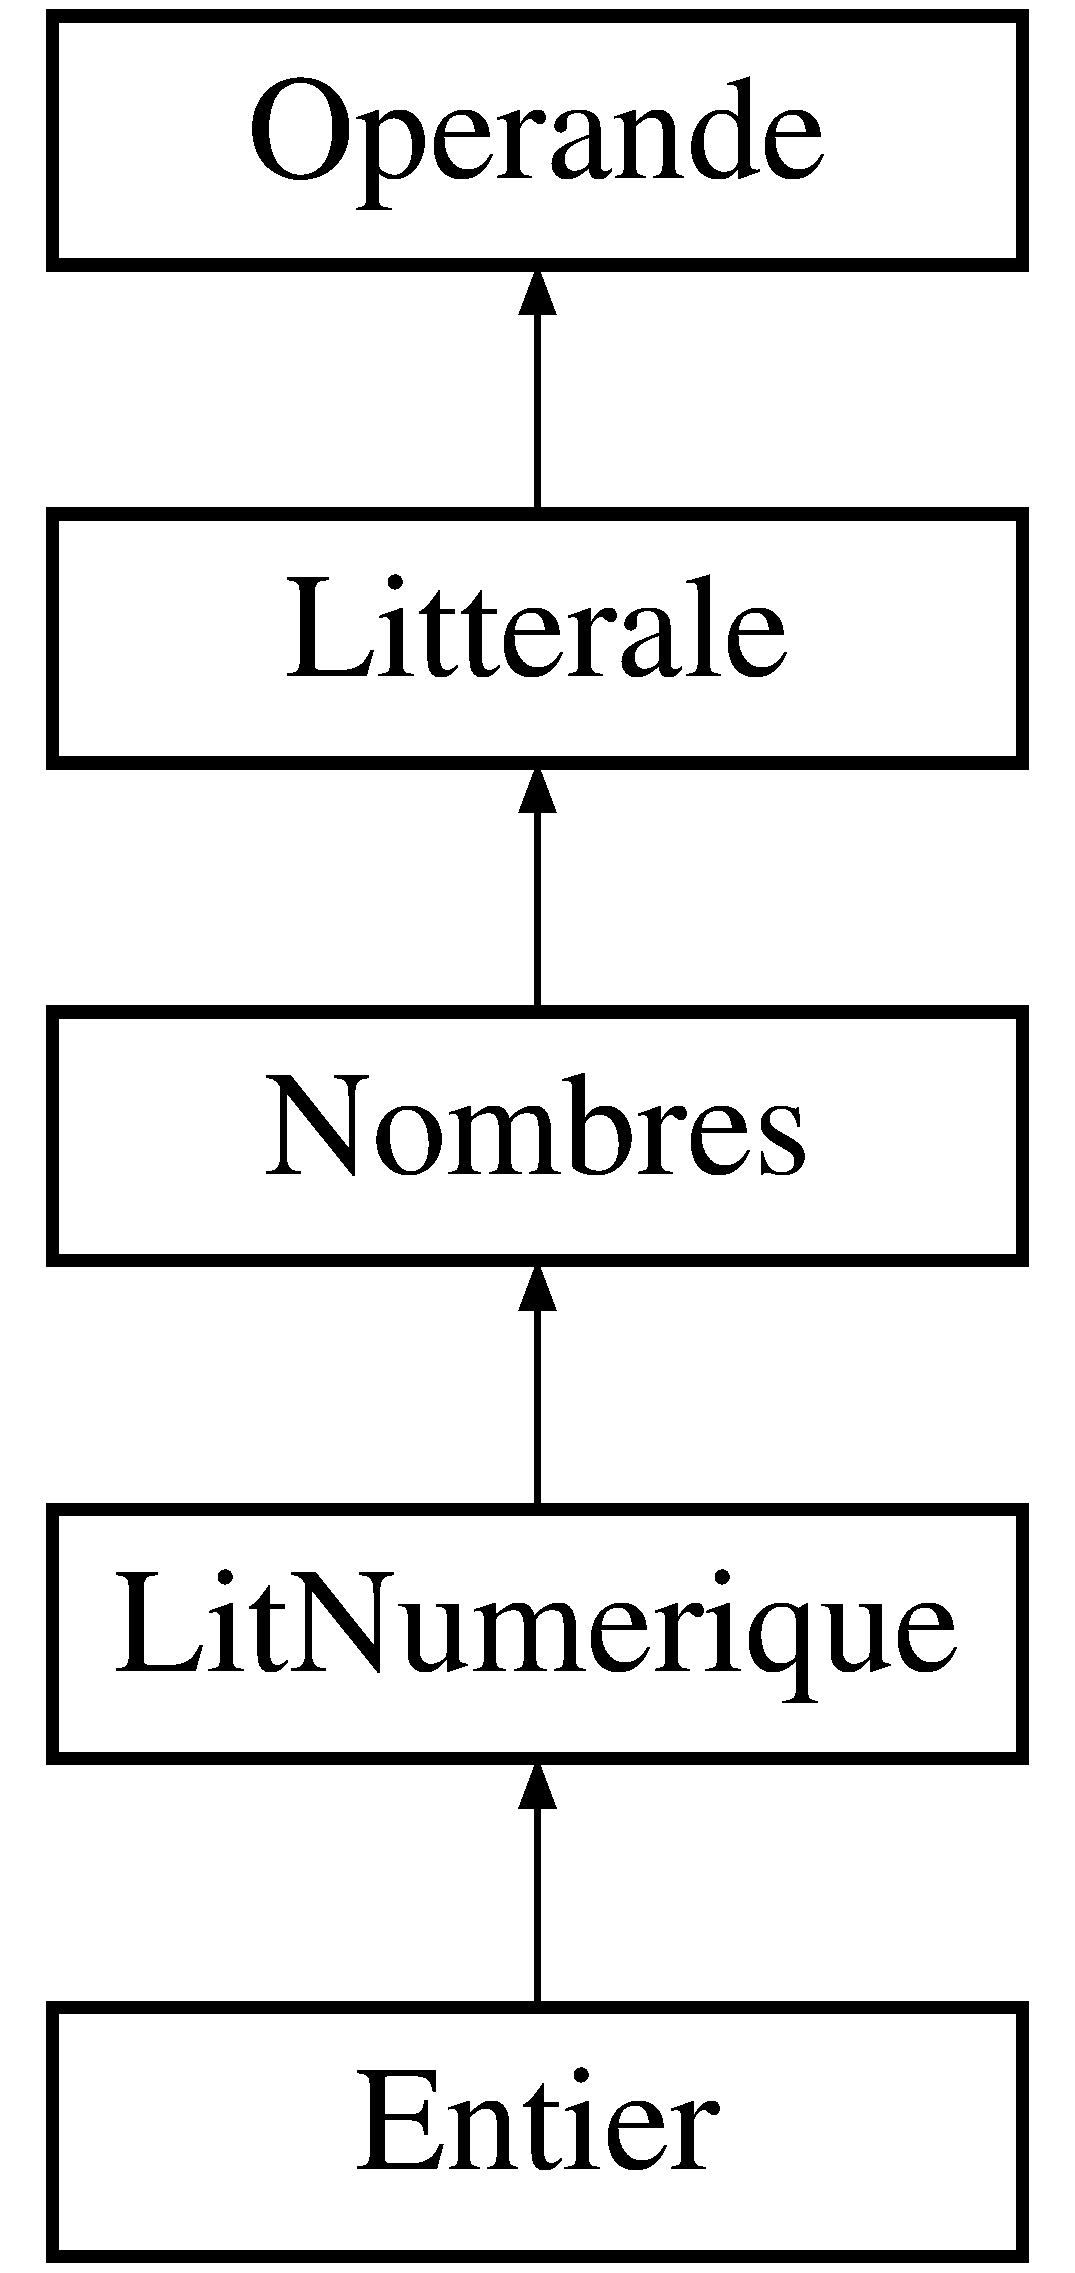
\includegraphics[height=5.000000cm]{class_entier}
\end{center}
\end{figure}
\subsection*{Public Member Functions}
\begin{DoxyCompactItemize}
\item 
\hyperlink{class_entier_a9ea07d2159b38f33cd78c19e432b5ad7}{Entier} (unsigned int va, const Q\+String \&na=\char`\"{}\char`\"{})
\item 
Q\+String \hyperlink{class_entier_aa960356dfeae8af6dfa2cd25136a1a6f}{to\+String} () const 
\item 
float \hyperlink{class_entier_abf00655fade13aac8b37a324e9bbca21}{get\+Value} () const 
\item 
unsigned int \hyperlink{class_entier_a539c8bf0d591a4fea2a007d1976a9e5b}{get\+Value\+Ent} () const 
\item 
void \hyperlink{class_entier_aad8b9c1da48b552657495e467eb50cde}{set\+Value} (unsigned int v)
\end{DoxyCompactItemize}
\subsection*{Additional Inherited Members}


\subsection{Detailed Description}


Definition at line 108 of file litterale.\+h.



\subsection{Constructor \& Destructor Documentation}
\index{Entier@{Entier}!Entier@{Entier}}
\index{Entier@{Entier}!Entier@{Entier}}
\subsubsection[{\texorpdfstring{Entier(unsigned int va, const Q\+String \&na="""")}{Entier(unsigned int va, const QString &na="")}}]{\setlength{\rightskip}{0pt plus 5cm}Entier\+::\+Entier (
\begin{DoxyParamCaption}
\item[{unsigned int}]{va, }
\item[{const Q\+String \&}]{na = {\ttfamily \char`\"{}\char`\"{}}}
\end{DoxyParamCaption}
)\hspace{0.3cm}{\ttfamily [inline]}}\hypertarget{class_entier_a9ea07d2159b38f33cd78c19e432b5ad7}{}\label{class_entier_a9ea07d2159b38f33cd78c19e432b5ad7}


Definition at line 112 of file litterale.\+h.



\subsection{Member Function Documentation}
\index{Entier@{Entier}!get\+Value@{get\+Value}}
\index{get\+Value@{get\+Value}!Entier@{Entier}}
\subsubsection[{\texorpdfstring{get\+Value() const }{getValue() const }}]{\setlength{\rightskip}{0pt plus 5cm}float Entier\+::get\+Value (
\begin{DoxyParamCaption}
{}
\end{DoxyParamCaption}
) const\hspace{0.3cm}{\ttfamily [virtual]}}\hypertarget{class_entier_abf00655fade13aac8b37a324e9bbca21}{}\label{class_entier_abf00655fade13aac8b37a324e9bbca21}


Implements \hyperlink{class_lit_numerique_ae7ecb1f7671754bc2155e35428e21124}{Lit\+Numerique}.



Definition at line 85 of file litterale.\+cpp.

\index{Entier@{Entier}!get\+Value\+Ent@{get\+Value\+Ent}}
\index{get\+Value\+Ent@{get\+Value\+Ent}!Entier@{Entier}}
\subsubsection[{\texorpdfstring{get\+Value\+Ent() const }{getValueEnt() const }}]{\setlength{\rightskip}{0pt plus 5cm}unsigned int Entier\+::get\+Value\+Ent (
\begin{DoxyParamCaption}
{}
\end{DoxyParamCaption}
) const\hspace{0.3cm}{\ttfamily [inline]}}\hypertarget{class_entier_a539c8bf0d591a4fea2a007d1976a9e5b}{}\label{class_entier_a539c8bf0d591a4fea2a007d1976a9e5b}


Definition at line 115 of file litterale.\+h.

\index{Entier@{Entier}!set\+Value@{set\+Value}}
\index{set\+Value@{set\+Value}!Entier@{Entier}}
\subsubsection[{\texorpdfstring{set\+Value(unsigned int v)}{setValue(unsigned int v)}}]{\setlength{\rightskip}{0pt plus 5cm}void Entier\+::set\+Value (
\begin{DoxyParamCaption}
\item[{unsigned int}]{v}
\end{DoxyParamCaption}
)\hspace{0.3cm}{\ttfamily [inline]}}\hypertarget{class_entier_aad8b9c1da48b552657495e467eb50cde}{}\label{class_entier_aad8b9c1da48b552657495e467eb50cde}


Definition at line 116 of file litterale.\+h.

\index{Entier@{Entier}!to\+String@{to\+String}}
\index{to\+String@{to\+String}!Entier@{Entier}}
\subsubsection[{\texorpdfstring{to\+String() const }{toString() const }}]{\setlength{\rightskip}{0pt plus 5cm}Q\+String Entier\+::to\+String (
\begin{DoxyParamCaption}
{}
\end{DoxyParamCaption}
) const\hspace{0.3cm}{\ttfamily [virtual]}}\hypertarget{class_entier_aa960356dfeae8af6dfa2cd25136a1a6f}{}\label{class_entier_aa960356dfeae8af6dfa2cd25136a1a6f}


Implements \hyperlink{class_lit_numerique_a6e3c66f0b484c5be954eb788a95c0d16}{Lit\+Numerique}.



Definition at line 77 of file litterale.\+cpp.



The documentation for this class was generated from the following files\+:\begin{DoxyCompactItemize}
\item 
\hyperlink{litterale_8h}{litterale.\+h}\item 
\hyperlink{litterale_8cpp}{litterale.\+cpp}\end{DoxyCompactItemize}

\hypertarget{class_item}{}\section{Item Class Reference}
\label{class_item}\index{Item@{Item}}


{\ttfamily \#include $<$pile.\+h$>$}

\subsection*{Public Member Functions}
\begin{DoxyCompactItemize}
\item 
\hyperlink{class_item_a297720c02984eab37332ae795d22189d}{Item} ()
\item 
void \hyperlink{class_item_a53ff859216bae7074ded5e949a7b7986}{set\+Litterale} (\hyperlink{class_litterale}{Litterale} \&e)
\item 
void \hyperlink{class_item_a24858085cb6b69b1776423bc9a6ce4ce}{raz} ()
\item 
\hyperlink{class_litterale}{Litterale} \& \hyperlink{class_item_a8a72e6b5449e462b75f4d1758debdbe9}{get\+Litterale} () const 
\end{DoxyCompactItemize}


\subsection{Detailed Description}


Definition at line 9 of file pile.\+h.



\subsection{Constructor \& Destructor Documentation}
\index{Item@{Item}!Item@{Item}}
\index{Item@{Item}!Item@{Item}}
\subsubsection[{\texorpdfstring{Item()}{Item()}}]{\setlength{\rightskip}{0pt plus 5cm}Item\+::\+Item (
\begin{DoxyParamCaption}
{}
\end{DoxyParamCaption}
)\hspace{0.3cm}{\ttfamily [inline]}}\hypertarget{class_item_a297720c02984eab37332ae795d22189d}{}\label{class_item_a297720c02984eab37332ae795d22189d}


Definition at line 12 of file pile.\+h.



\subsection{Member Function Documentation}
\index{Item@{Item}!get\+Litterale@{get\+Litterale}}
\index{get\+Litterale@{get\+Litterale}!Item@{Item}}
\subsubsection[{\texorpdfstring{get\+Litterale() const }{getLitterale() const }}]{\setlength{\rightskip}{0pt plus 5cm}{\bf Litterale} \& Item\+::get\+Litterale (
\begin{DoxyParamCaption}
{}
\end{DoxyParamCaption}
) const}\hypertarget{class_item_a8a72e6b5449e462b75f4d1758debdbe9}{}\label{class_item_a8a72e6b5449e462b75f4d1758debdbe9}


Definition at line 210 of file computer.\+cpp.

\index{Item@{Item}!raz@{raz}}
\index{raz@{raz}!Item@{Item}}
\subsubsection[{\texorpdfstring{raz()}{raz()}}]{\setlength{\rightskip}{0pt plus 5cm}void Item\+::raz (
\begin{DoxyParamCaption}
{}
\end{DoxyParamCaption}
)\hspace{0.3cm}{\ttfamily [inline]}}\hypertarget{class_item_a24858085cb6b69b1776423bc9a6ce4ce}{}\label{class_item_a24858085cb6b69b1776423bc9a6ce4ce}


Definition at line 14 of file pile.\+h.

\index{Item@{Item}!set\+Litterale@{set\+Litterale}}
\index{set\+Litterale@{set\+Litterale}!Item@{Item}}
\subsubsection[{\texorpdfstring{set\+Litterale(\+Litterale \&e)}{setLitterale(Litterale &e)}}]{\setlength{\rightskip}{0pt plus 5cm}void Item\+::set\+Litterale (
\begin{DoxyParamCaption}
\item[{{\bf Litterale} \&}]{e}
\end{DoxyParamCaption}
)\hspace{0.3cm}{\ttfamily [inline]}}\hypertarget{class_item_a53ff859216bae7074ded5e949a7b7986}{}\label{class_item_a53ff859216bae7074ded5e949a7b7986}


Definition at line 13 of file pile.\+h.



The documentation for this class was generated from the following files\+:\begin{DoxyCompactItemize}
\item 
\hyperlink{pile_8h}{pile.\+h}\item 
\hyperlink{computer_8cpp}{computer.\+cpp}\end{DoxyCompactItemize}

\hypertarget{class_pile_1_1iterator}{}\section{Pile\+:\+:iterator Class Reference}
\label{class_pile_1_1iterator}\index{Pile\+::iterator@{Pile\+::iterator}}


{\ttfamily \#include $<$pile.\+h$>$}

\subsection*{Public Member Functions}
\begin{DoxyCompactItemize}
\item 
\hyperlink{class_pile_1_1iterator_a840f05175548dd9ac7bb595206f0044f}{iterator} ()
\item 
\hyperlink{class_litterale}{Litterale} \& \hyperlink{class_pile_1_1iterator_a5a84d0211e5cfb4ddb45661d7e940e87}{operator$\ast$} () const 
\item 
bool \hyperlink{class_pile_1_1iterator_abfe0e25a2ebc5f3188c7a13f09d19129}{operator!=} (\hyperlink{class_pile_1_1iterator}{iterator} it) const 
\item 
\hyperlink{class_pile_1_1iterator}{iterator} \& \hyperlink{class_pile_1_1iterator_a05b171f7019504d6fb1b6a9a183bd75b}{operator++} ()
\end{DoxyCompactItemize}
\subsection*{Friends}
\begin{DoxyCompactItemize}
\item 
class \hyperlink{class_pile_1_1iterator_a77806361379cf369e95d2b4346c7e28a}{Pile}
\end{DoxyCompactItemize}


\subsection{Detailed Description}


Definition at line 42 of file pile.\+h.



\subsection{Constructor \& Destructor Documentation}
\index{Pile\+::iterator@{Pile\+::iterator}!iterator@{iterator}}
\index{iterator@{iterator}!Pile\+::iterator@{Pile\+::iterator}}
\subsubsection[{\texorpdfstring{iterator()}{iterator()}}]{\setlength{\rightskip}{0pt plus 5cm}Pile\+::iterator\+::iterator (
\begin{DoxyParamCaption}
{}
\end{DoxyParamCaption}
)\hspace{0.3cm}{\ttfamily [inline]}}\hypertarget{class_pile_1_1iterator_a840f05175548dd9ac7bb595206f0044f}{}\label{class_pile_1_1iterator_a840f05175548dd9ac7bb595206f0044f}


Definition at line 47 of file pile.\+h.



\subsection{Member Function Documentation}
\index{Pile\+::iterator@{Pile\+::iterator}!operator"!=@{operator"!=}}
\index{operator"!=@{operator"!=}!Pile\+::iterator@{Pile\+::iterator}}
\subsubsection[{\texorpdfstring{operator"!=(iterator it) const }{operator!=(iterator it) const }}]{\setlength{\rightskip}{0pt plus 5cm}bool Pile\+::iterator\+::operator!= (
\begin{DoxyParamCaption}
\item[{{\bf iterator}}]{it}
\end{DoxyParamCaption}
) const\hspace{0.3cm}{\ttfamily [inline]}}\hypertarget{class_pile_1_1iterator_abfe0e25a2ebc5f3188c7a13f09d19129}{}\label{class_pile_1_1iterator_abfe0e25a2ebc5f3188c7a13f09d19129}


Definition at line 49 of file pile.\+h.

\index{Pile\+::iterator@{Pile\+::iterator}!operator$\ast$@{operator$\ast$}}
\index{operator$\ast$@{operator$\ast$}!Pile\+::iterator@{Pile\+::iterator}}
\subsubsection[{\texorpdfstring{operator$\ast$() const }{operator*() const }}]{\setlength{\rightskip}{0pt plus 5cm}{\bf Litterale}\& Pile\+::iterator\+::operator$\ast$ (
\begin{DoxyParamCaption}
{}
\end{DoxyParamCaption}
) const\hspace{0.3cm}{\ttfamily [inline]}}\hypertarget{class_pile_1_1iterator_a5a84d0211e5cfb4ddb45661d7e940e87}{}\label{class_pile_1_1iterator_a5a84d0211e5cfb4ddb45661d7e940e87}


Definition at line 48 of file pile.\+h.

\index{Pile\+::iterator@{Pile\+::iterator}!operator++@{operator++}}
\index{operator++@{operator++}!Pile\+::iterator@{Pile\+::iterator}}
\subsubsection[{\texorpdfstring{operator++()}{operator++()}}]{\setlength{\rightskip}{0pt plus 5cm}{\bf iterator}\& Pile\+::iterator\+::operator++ (
\begin{DoxyParamCaption}
{}
\end{DoxyParamCaption}
)\hspace{0.3cm}{\ttfamily [inline]}}\hypertarget{class_pile_1_1iterator_a05b171f7019504d6fb1b6a9a183bd75b}{}\label{class_pile_1_1iterator_a05b171f7019504d6fb1b6a9a183bd75b}


Definition at line 50 of file pile.\+h.



\subsection{Friends And Related Function Documentation}
\index{Pile\+::iterator@{Pile\+::iterator}!Pile@{Pile}}
\index{Pile@{Pile}!Pile\+::iterator@{Pile\+::iterator}}
\subsubsection[{\texorpdfstring{Pile}{Pile}}]{\setlength{\rightskip}{0pt plus 5cm}friend class {\bf Pile}\hspace{0.3cm}{\ttfamily [friend]}}\hypertarget{class_pile_1_1iterator_a77806361379cf369e95d2b4346c7e28a}{}\label{class_pile_1_1iterator_a77806361379cf369e95d2b4346c7e28a}


Definition at line 45 of file pile.\+h.



The documentation for this class was generated from the following file\+:\begin{DoxyCompactItemize}
\item 
\hyperlink{pile_8h}{pile.\+h}\end{DoxyCompactItemize}

\hypertarget{class_litterale_manager_1_1iterator}{}\section{Litterale\+Manager\+:\+:iterator Class Reference}
\label{class_litterale_manager_1_1iterator}\index{Litterale\+Manager\+::iterator@{Litterale\+Manager\+::iterator}}


{\ttfamily \#include $<$computer.\+h$>$}

\subsection*{Public Member Functions}
\begin{DoxyCompactItemize}
\item 
\hyperlink{class_litterale_manager_1_1iterator_ac9a388cca532cb873bcf1ec5ef768dcc}{iterator} ()
\item 
\hyperlink{class_litterale}{Litterale} \& \hyperlink{class_litterale_manager_1_1iterator_ac92c56aa84ef69cfe9aafbe42b721b6a}{operator$\ast$} () const 
\item 
bool \hyperlink{class_litterale_manager_1_1iterator_ad319aadb70ba8482de219f7ef826242c}{operator!=} (\hyperlink{class_litterale_manager_1_1iterator}{iterator} it) const 
\item 
\hyperlink{class_litterale_manager_1_1iterator}{iterator} \& \hyperlink{class_litterale_manager_1_1iterator_a9fdfe99fd9c3eb4e57445fe8c1a1cf2b}{operator++} ()
\end{DoxyCompactItemize}
\subsection*{Friends}
\begin{DoxyCompactItemize}
\item 
class \hyperlink{class_litterale_manager_1_1iterator_a0aab3199db1ebeb99e33e66b9cf8e975}{Litterale\+Manager}
\end{DoxyCompactItemize}


\subsection{Detailed Description}


Definition at line 44 of file computer.\+h.



\subsection{Constructor \& Destructor Documentation}
\index{Litterale\+Manager\+::iterator@{Litterale\+Manager\+::iterator}!iterator@{iterator}}
\index{iterator@{iterator}!Litterale\+Manager\+::iterator@{Litterale\+Manager\+::iterator}}
\subsubsection[{\texorpdfstring{iterator()}{iterator()}}]{\setlength{\rightskip}{0pt plus 5cm}Litterale\+Manager\+::iterator\+::iterator (
\begin{DoxyParamCaption}
{}
\end{DoxyParamCaption}
)\hspace{0.3cm}{\ttfamily [inline]}}\hypertarget{class_litterale_manager_1_1iterator_ac9a388cca532cb873bcf1ec5ef768dcc}{}\label{class_litterale_manager_1_1iterator_ac9a388cca532cb873bcf1ec5ef768dcc}


Definition at line 49 of file computer.\+h.



\subsection{Member Function Documentation}
\index{Litterale\+Manager\+::iterator@{Litterale\+Manager\+::iterator}!operator"!=@{operator"!=}}
\index{operator"!=@{operator"!=}!Litterale\+Manager\+::iterator@{Litterale\+Manager\+::iterator}}
\subsubsection[{\texorpdfstring{operator"!=(iterator it) const }{operator!=(iterator it) const }}]{\setlength{\rightskip}{0pt plus 5cm}bool Litterale\+Manager\+::iterator\+::operator!= (
\begin{DoxyParamCaption}
\item[{{\bf iterator}}]{it}
\end{DoxyParamCaption}
) const\hspace{0.3cm}{\ttfamily [inline]}}\hypertarget{class_litterale_manager_1_1iterator_ad319aadb70ba8482de219f7ef826242c}{}\label{class_litterale_manager_1_1iterator_ad319aadb70ba8482de219f7ef826242c}


Definition at line 51 of file computer.\+h.

\index{Litterale\+Manager\+::iterator@{Litterale\+Manager\+::iterator}!operator$\ast$@{operator$\ast$}}
\index{operator$\ast$@{operator$\ast$}!Litterale\+Manager\+::iterator@{Litterale\+Manager\+::iterator}}
\subsubsection[{\texorpdfstring{operator$\ast$() const }{operator*() const }}]{\setlength{\rightskip}{0pt plus 5cm}{\bf Litterale}\& Litterale\+Manager\+::iterator\+::operator$\ast$ (
\begin{DoxyParamCaption}
{}
\end{DoxyParamCaption}
) const\hspace{0.3cm}{\ttfamily [inline]}}\hypertarget{class_litterale_manager_1_1iterator_ac92c56aa84ef69cfe9aafbe42b721b6a}{}\label{class_litterale_manager_1_1iterator_ac92c56aa84ef69cfe9aafbe42b721b6a}


Definition at line 50 of file computer.\+h.

\index{Litterale\+Manager\+::iterator@{Litterale\+Manager\+::iterator}!operator++@{operator++}}
\index{operator++@{operator++}!Litterale\+Manager\+::iterator@{Litterale\+Manager\+::iterator}}
\subsubsection[{\texorpdfstring{operator++()}{operator++()}}]{\setlength{\rightskip}{0pt plus 5cm}{\bf iterator}\& Litterale\+Manager\+::iterator\+::operator++ (
\begin{DoxyParamCaption}
{}
\end{DoxyParamCaption}
)\hspace{0.3cm}{\ttfamily [inline]}}\hypertarget{class_litterale_manager_1_1iterator_a9fdfe99fd9c3eb4e57445fe8c1a1cf2b}{}\label{class_litterale_manager_1_1iterator_a9fdfe99fd9c3eb4e57445fe8c1a1cf2b}


Definition at line 52 of file computer.\+h.



\subsection{Friends And Related Function Documentation}
\index{Litterale\+Manager\+::iterator@{Litterale\+Manager\+::iterator}!Litterale\+Manager@{Litterale\+Manager}}
\index{Litterale\+Manager@{Litterale\+Manager}!Litterale\+Manager\+::iterator@{Litterale\+Manager\+::iterator}}
\subsubsection[{\texorpdfstring{Litterale\+Manager}{LitteraleManager}}]{\setlength{\rightskip}{0pt plus 5cm}friend class {\bf Litterale\+Manager}\hspace{0.3cm}{\ttfamily [friend]}}\hypertarget{class_litterale_manager_1_1iterator_a0aab3199db1ebeb99e33e66b9cf8e975}{}\label{class_litterale_manager_1_1iterator_a0aab3199db1ebeb99e33e66b9cf8e975}


Definition at line 47 of file computer.\+h.



The documentation for this class was generated from the following file\+:\begin{DoxyCompactItemize}
\item 
\hyperlink{computer_8h}{computer.\+h}\end{DoxyCompactItemize}

\hypertarget{class_lit_atome}{}\section{Lit\+Atome Class Reference}
\label{class_lit_atome}\index{Lit\+Atome@{Lit\+Atome}}


{\ttfamily \#include $<$litterale.\+h$>$}

Inheritance diagram for Lit\+Atome\+:\begin{figure}[H]
\begin{center}
\leavevmode
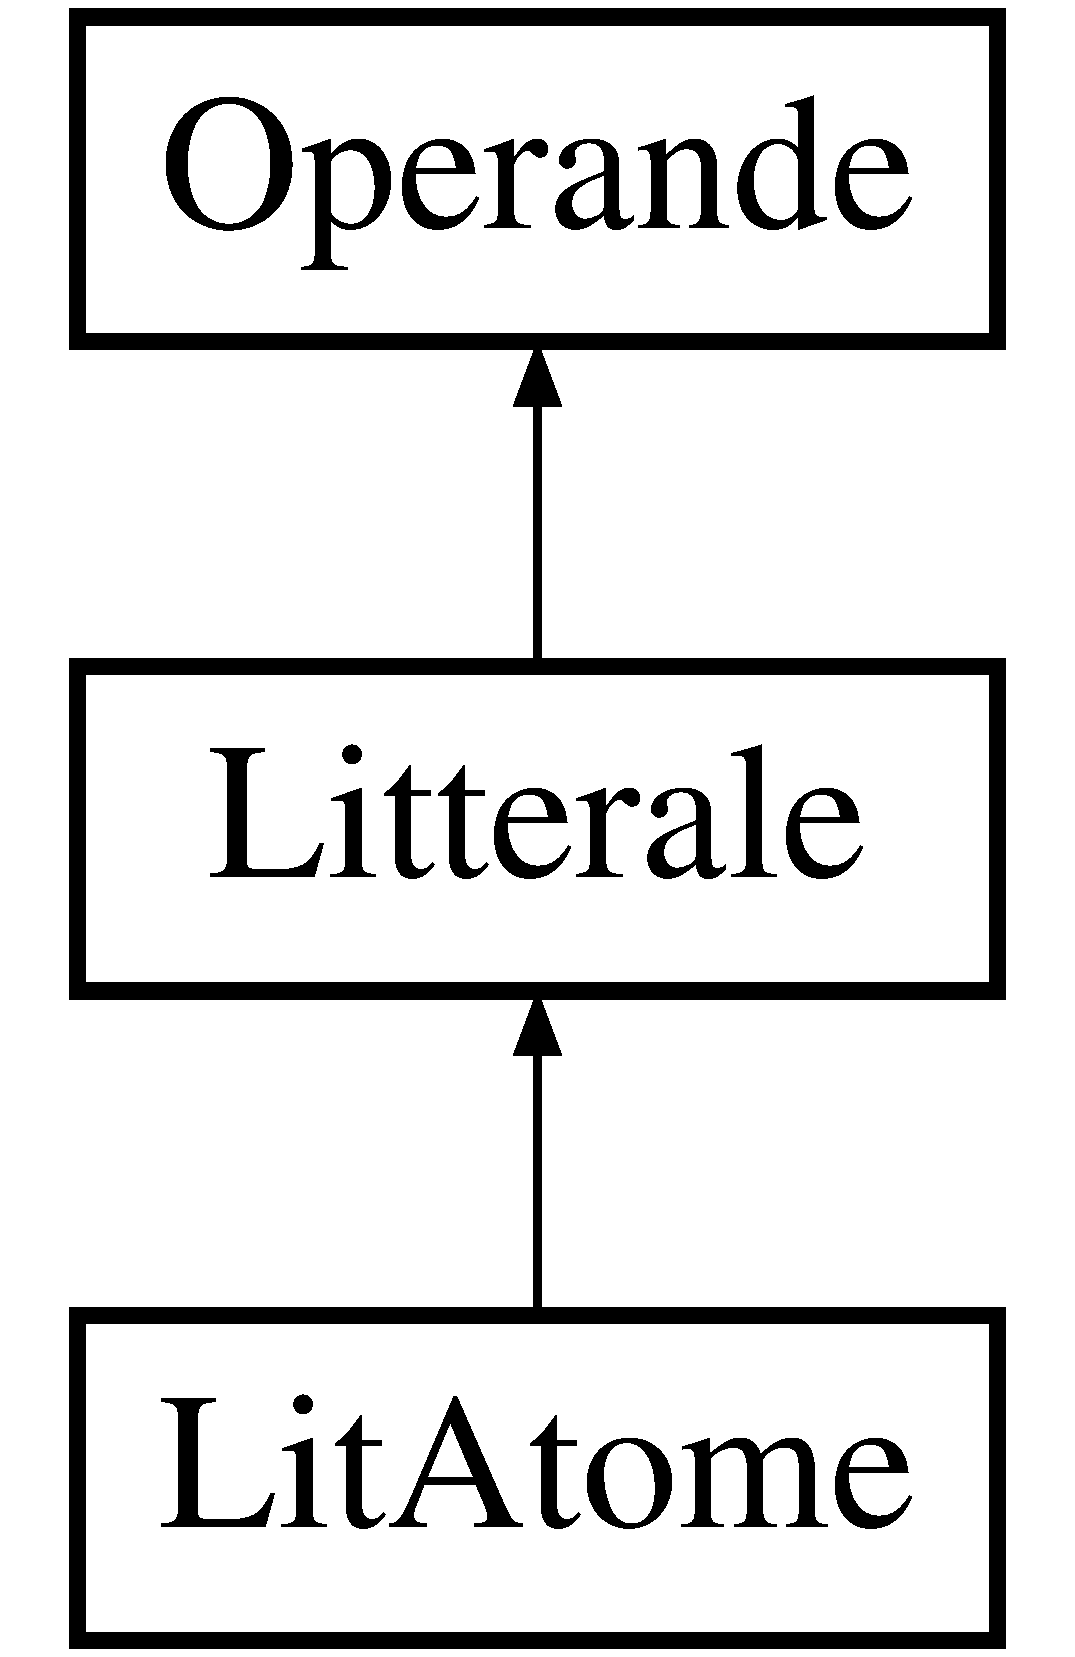
\includegraphics[height=3.000000cm]{class_lit_atome}
\end{center}
\end{figure}
\subsection*{Public Member Functions}
\begin{DoxyCompactItemize}
\item 
\hyperlink{class_lit_atome_a8bc929ccdcc5d9f145d728ce889d1341}{Lit\+Atome} (const Q\+String \&va, const Q\+String \&na=\char`\"{}\char`\"{})
\item 
const Q\+String \& \hyperlink{class_lit_atome_a689b894878fe347a6c622836b6d6d5fb}{get\+Value} () const 
\item 
Q\+String \hyperlink{class_lit_atome_abbe47368e149ae5a9744bc7188df1cc8}{to\+String} () const 
\end{DoxyCompactItemize}
\subsection*{Additional Inherited Members}


\subsection{Detailed Description}


Definition at line 78 of file litterale.\+h.



\subsection{Constructor \& Destructor Documentation}
\index{Lit\+Atome@{Lit\+Atome}!Lit\+Atome@{Lit\+Atome}}
\index{Lit\+Atome@{Lit\+Atome}!Lit\+Atome@{Lit\+Atome}}
\subsubsection[{\texorpdfstring{Lit\+Atome(const Q\+String \&va, const Q\+String \&na="""")}{LitAtome(const QString &va, const QString &na="")}}]{\setlength{\rightskip}{0pt plus 5cm}Lit\+Atome\+::\+Lit\+Atome (
\begin{DoxyParamCaption}
\item[{const Q\+String \&}]{va, }
\item[{const Q\+String \&}]{na = {\ttfamily \char`\"{}\char`\"{}}}
\end{DoxyParamCaption}
)\hspace{0.3cm}{\ttfamily [inline]}}\hypertarget{class_lit_atome_a8bc929ccdcc5d9f145d728ce889d1341}{}\label{class_lit_atome_a8bc929ccdcc5d9f145d728ce889d1341}


Definition at line 81 of file litterale.\+h.



\subsection{Member Function Documentation}
\index{Lit\+Atome@{Lit\+Atome}!get\+Value@{get\+Value}}
\index{get\+Value@{get\+Value}!Lit\+Atome@{Lit\+Atome}}
\subsubsection[{\texorpdfstring{get\+Value() const }{getValue() const }}]{\setlength{\rightskip}{0pt plus 5cm}const Q\+String\& Lit\+Atome\+::get\+Value (
\begin{DoxyParamCaption}
{}
\end{DoxyParamCaption}
) const\hspace{0.3cm}{\ttfamily [inline]}}\hypertarget{class_lit_atome_a689b894878fe347a6c622836b6d6d5fb}{}\label{class_lit_atome_a689b894878fe347a6c622836b6d6d5fb}


Definition at line 82 of file litterale.\+h.

\index{Lit\+Atome@{Lit\+Atome}!to\+String@{to\+String}}
\index{to\+String@{to\+String}!Lit\+Atome@{Lit\+Atome}}
\subsubsection[{\texorpdfstring{to\+String() const }{toString() const }}]{\setlength{\rightskip}{0pt plus 5cm}Q\+String Lit\+Atome\+::to\+String (
\begin{DoxyParamCaption}
{}
\end{DoxyParamCaption}
) const\hspace{0.3cm}{\ttfamily [virtual]}}\hypertarget{class_lit_atome_abbe47368e149ae5a9744bc7188df1cc8}{}\label{class_lit_atome_abbe47368e149ae5a9744bc7188df1cc8}


Implements \hyperlink{class_litterale_a3b427621132af2903259390143d1b16d}{Litterale}.



Definition at line 59 of file litterale.\+cpp.



The documentation for this class was generated from the following files\+:\begin{DoxyCompactItemize}
\item 
\hyperlink{litterale_8h}{litterale.\+h}\item 
\hyperlink{litterale_8cpp}{litterale.\+cpp}\end{DoxyCompactItemize}

\hypertarget{class_lit_expression}{}\section{Lit\+Expression Class Reference}
\label{class_lit_expression}\index{Lit\+Expression@{Lit\+Expression}}


{\ttfamily \#include $<$litterale.\+h$>$}

Inheritance diagram for Lit\+Expression\+:\begin{figure}[H]
\begin{center}
\leavevmode
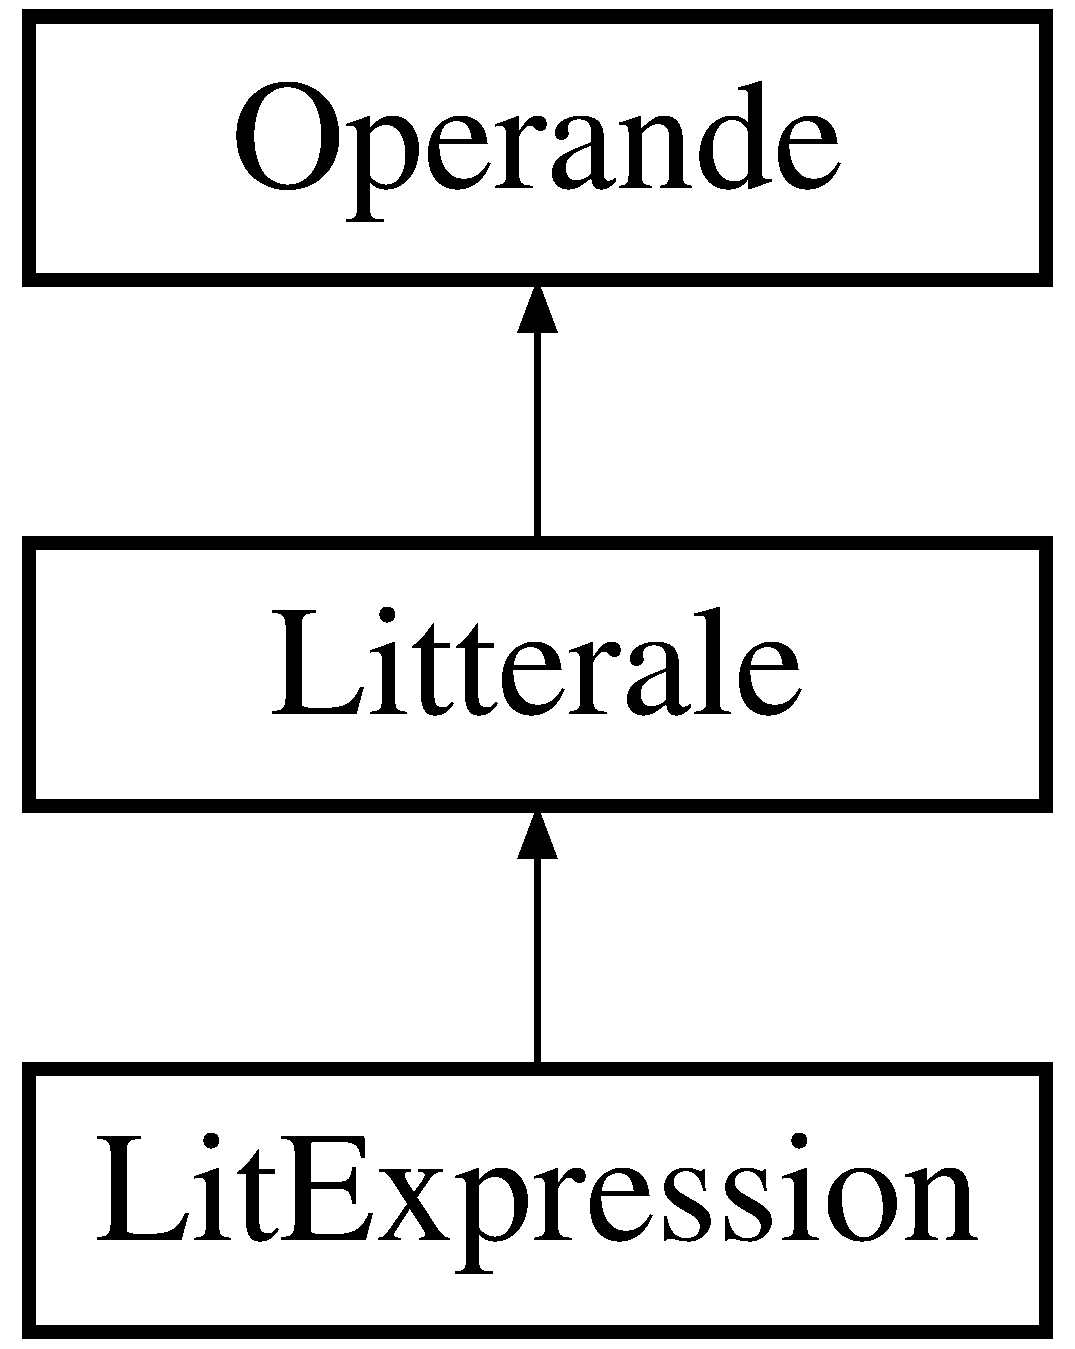
\includegraphics[height=3.000000cm]{class_lit_expression}
\end{center}
\end{figure}
\subsection*{Public Member Functions}
\begin{DoxyCompactItemize}
\item 
\hyperlink{class_lit_expression_a5d6cb1828c33a9c39684766c21042216}{Lit\+Expression} (const Q\+String \&str, const Q\+String \&na=\char`\"{}\char`\"{})
\item 
\hyperlink{class_litterale}{Litterale} $\ast$ \hyperlink{class_lit_expression_aa4b5ba342bdf239612d733d7f8e5319c}{get\+Value} () const 
\item 
void \hyperlink{class_lit_expression_a60a52c1344ff29fa1576720bc60c0577}{set\+Vector} (Q\+Vector$<$ \hyperlink{class_operande}{Operande} $\ast$ $>$ \&vec)
\item 
Q\+Vector$<$ \hyperlink{class_operande}{Operande} $\ast$ $>$ \& \hyperlink{class_lit_expression_a9ba612027808bbc67d762e7592332d79}{get\+Vector} ()
\item 
Q\+String \hyperlink{class_lit_expression_a108f8809e4ca49343426c9d0c30c28c4}{to\+String} () const 
\item 
void \hyperlink{class_lit_expression_a6673aba807725a2e1820af3bfeb8cf36}{verif\+Neg} () const 
\end{DoxyCompactItemize}
\subsection*{Additional Inherited Members}


\subsection{Detailed Description}


Definition at line 63 of file litterale.\+h.



\subsection{Constructor \& Destructor Documentation}
\index{Lit\+Expression@{Lit\+Expression}!Lit\+Expression@{Lit\+Expression}}
\index{Lit\+Expression@{Lit\+Expression}!Lit\+Expression@{Lit\+Expression}}
\subsubsection[{\texorpdfstring{Lit\+Expression(const Q\+String \&str, const Q\+String \&na="""")}{LitExpression(const QString &str, const QString &na="")}}]{\setlength{\rightskip}{0pt plus 5cm}Lit\+Expression\+::\+Lit\+Expression (
\begin{DoxyParamCaption}
\item[{const Q\+String \&}]{str, }
\item[{const Q\+String \&}]{na = {\ttfamily \char`\"{}\char`\"{}}}
\end{DoxyParamCaption}
)}\hypertarget{class_lit_expression_a5d6cb1828c33a9c39684766c21042216}{}\label{class_lit_expression_a5d6cb1828c33a9c39684766c21042216}


Definition at line 35 of file litterale.\+cpp.



\subsection{Member Function Documentation}
\index{Lit\+Expression@{Lit\+Expression}!get\+Value@{get\+Value}}
\index{get\+Value@{get\+Value}!Lit\+Expression@{Lit\+Expression}}
\subsubsection[{\texorpdfstring{get\+Value() const }{getValue() const }}]{\setlength{\rightskip}{0pt plus 5cm}{\bf Litterale}$\ast$ Lit\+Expression\+::get\+Value (
\begin{DoxyParamCaption}
{}
\end{DoxyParamCaption}
) const}\hypertarget{class_lit_expression_aa4b5ba342bdf239612d733d7f8e5319c}{}\label{class_lit_expression_aa4b5ba342bdf239612d733d7f8e5319c}
\index{Lit\+Expression@{Lit\+Expression}!get\+Vector@{get\+Vector}}
\index{get\+Vector@{get\+Vector}!Lit\+Expression@{Lit\+Expression}}
\subsubsection[{\texorpdfstring{get\+Vector()}{getVector()}}]{\setlength{\rightskip}{0pt plus 5cm}Q\+Vector$<${\bf Operande}$\ast$$>$\& Lit\+Expression\+::get\+Vector (
\begin{DoxyParamCaption}
{}
\end{DoxyParamCaption}
)\hspace{0.3cm}{\ttfamily [inline]}}\hypertarget{class_lit_expression_a9ba612027808bbc67d762e7592332d79}{}\label{class_lit_expression_a9ba612027808bbc67d762e7592332d79}


Definition at line 72 of file litterale.\+h.

\index{Lit\+Expression@{Lit\+Expression}!set\+Vector@{set\+Vector}}
\index{set\+Vector@{set\+Vector}!Lit\+Expression@{Lit\+Expression}}
\subsubsection[{\texorpdfstring{set\+Vector(\+Q\+Vector$<$ Operande $\ast$ $>$ \&vec)}{setVector(QVector< Operande * > &vec)}}]{\setlength{\rightskip}{0pt plus 5cm}void Lit\+Expression\+::set\+Vector (
\begin{DoxyParamCaption}
\item[{Q\+Vector$<$ {\bf Operande} $\ast$ $>$ \&}]{vec}
\end{DoxyParamCaption}
)\hspace{0.3cm}{\ttfamily [inline]}}\hypertarget{class_lit_expression_a60a52c1344ff29fa1576720bc60c0577}{}\label{class_lit_expression_a60a52c1344ff29fa1576720bc60c0577}


Definition at line 71 of file litterale.\+h.

\index{Lit\+Expression@{Lit\+Expression}!to\+String@{to\+String}}
\index{to\+String@{to\+String}!Lit\+Expression@{Lit\+Expression}}
\subsubsection[{\texorpdfstring{to\+String() const }{toString() const }}]{\setlength{\rightskip}{0pt plus 5cm}Q\+String Lit\+Expression\+::to\+String (
\begin{DoxyParamCaption}
{}
\end{DoxyParamCaption}
) const\hspace{0.3cm}{\ttfamily [virtual]}}\hypertarget{class_lit_expression_a108f8809e4ca49343426c9d0c30c28c4}{}\label{class_lit_expression_a108f8809e4ca49343426c9d0c30c28c4}


Implements \hyperlink{class_litterale_a3b427621132af2903259390143d1b16d}{Litterale}.



Definition at line 53 of file litterale.\+cpp.

\index{Lit\+Expression@{Lit\+Expression}!verif\+Neg@{verif\+Neg}}
\index{verif\+Neg@{verif\+Neg}!Lit\+Expression@{Lit\+Expression}}
\subsubsection[{\texorpdfstring{verif\+Neg() const }{verifNeg() const }}]{\setlength{\rightskip}{0pt plus 5cm}void Lit\+Expression\+::verif\+Neg (
\begin{DoxyParamCaption}
{}
\end{DoxyParamCaption}
) const}\hypertarget{class_lit_expression_a6673aba807725a2e1820af3bfeb8cf36}{}\label{class_lit_expression_a6673aba807725a2e1820af3bfeb8cf36}


The documentation for this class was generated from the following files\+:\begin{DoxyCompactItemize}
\item 
\hyperlink{litterale_8h}{litterale.\+h}\item 
\hyperlink{litterale_8cpp}{litterale.\+cpp}\end{DoxyCompactItemize}

\hypertarget{class_lit_numerique}{}\section{Lit\+Numerique Class Reference}
\label{class_lit_numerique}\index{Lit\+Numerique@{Lit\+Numerique}}


{\ttfamily \#include $<$litterale.\+h$>$}

Inheritance diagram for Lit\+Numerique\+:\begin{figure}[H]
\begin{center}
\leavevmode
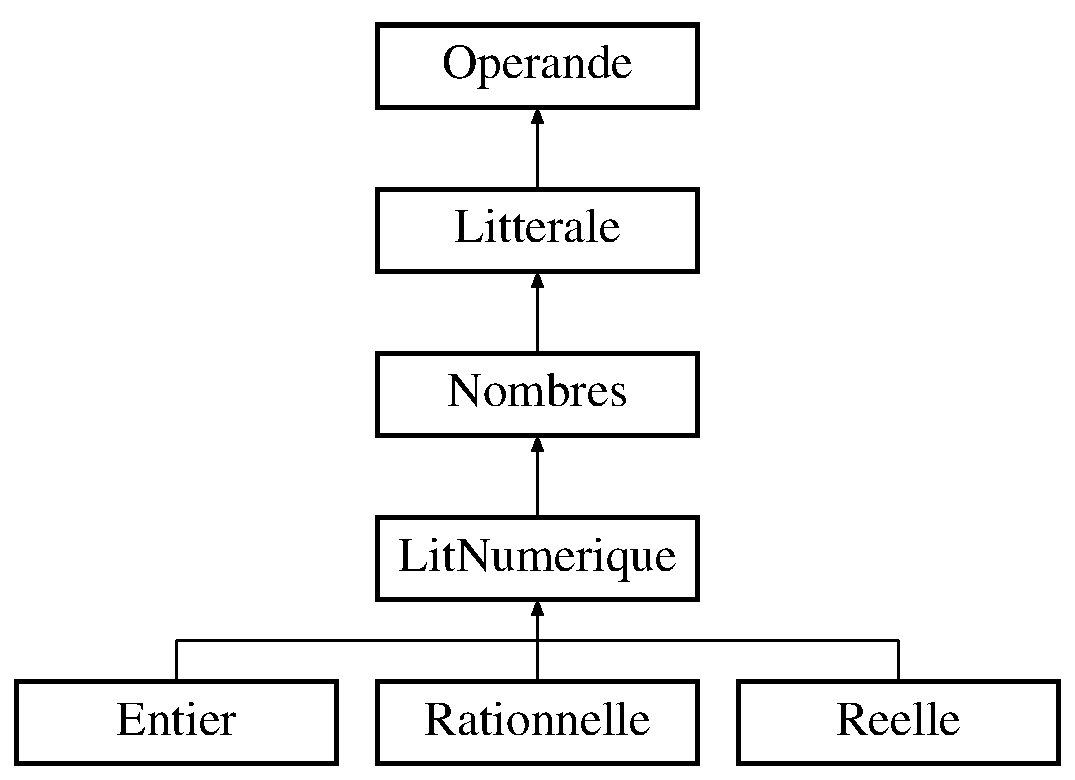
\includegraphics[height=5.000000cm]{class_lit_numerique}
\end{center}
\end{figure}
\subsection*{Public Member Functions}
\begin{DoxyCompactItemize}
\item 
\hyperlink{class_lit_numerique_a156cf838921ef4b54a1ce60d450dc32e}{Lit\+Numerique} (const Q\+String \&na=\char`\"{}\char`\"{})
\item 
virtual \hyperlink{class_lit_numerique_a7b49818486bc94d0a2fe5fb503184dd5}{$\sim$\+Lit\+Numerique} ()
\item 
virtual Q\+String \hyperlink{class_lit_numerique_a6e3c66f0b484c5be954eb788a95c0d16}{to\+String} () const  =0
\item 
virtual float \hyperlink{class_lit_numerique_ae7ecb1f7671754bc2155e35428e21124}{get\+Value} () const  =0
\end{DoxyCompactItemize}
\subsection*{Additional Inherited Members}


\subsection{Detailed Description}


Definition at line 97 of file litterale.\+h.



\subsection{Constructor \& Destructor Documentation}
\index{Lit\+Numerique@{Lit\+Numerique}!Lit\+Numerique@{Lit\+Numerique}}
\index{Lit\+Numerique@{Lit\+Numerique}!Lit\+Numerique@{Lit\+Numerique}}
\subsubsection[{\texorpdfstring{Lit\+Numerique(const Q\+String \&na="""")}{LitNumerique(const QString &na="")}}]{\setlength{\rightskip}{0pt plus 5cm}Lit\+Numerique\+::\+Lit\+Numerique (
\begin{DoxyParamCaption}
\item[{const Q\+String \&}]{na = {\ttfamily \char`\"{}\char`\"{}}}
\end{DoxyParamCaption}
)\hspace{0.3cm}{\ttfamily [inline]}}\hypertarget{class_lit_numerique_a156cf838921ef4b54a1ce60d450dc32e}{}\label{class_lit_numerique_a156cf838921ef4b54a1ce60d450dc32e}


Definition at line 101 of file litterale.\+h.

\index{Lit\+Numerique@{Lit\+Numerique}!````~Lit\+Numerique@{$\sim$\+Lit\+Numerique}}
\index{````~Lit\+Numerique@{$\sim$\+Lit\+Numerique}!Lit\+Numerique@{Lit\+Numerique}}
\subsubsection[{\texorpdfstring{$\sim$\+Lit\+Numerique()}{~LitNumerique()}}]{\setlength{\rightskip}{0pt plus 5cm}Lit\+Numerique\+::$\sim$\+Lit\+Numerique (
\begin{DoxyParamCaption}
{}
\end{DoxyParamCaption}
)\hspace{0.3cm}{\ttfamily [virtual]}}\hypertarget{class_lit_numerique_a7b49818486bc94d0a2fe5fb503184dd5}{}\label{class_lit_numerique_a7b49818486bc94d0a2fe5fb503184dd5}


Definition at line 72 of file litterale.\+cpp.



\subsection{Member Function Documentation}
\index{Lit\+Numerique@{Lit\+Numerique}!get\+Value@{get\+Value}}
\index{get\+Value@{get\+Value}!Lit\+Numerique@{Lit\+Numerique}}
\subsubsection[{\texorpdfstring{get\+Value() const  =0}{getValue() const  =0}}]{\setlength{\rightskip}{0pt plus 5cm}virtual float Lit\+Numerique\+::get\+Value (
\begin{DoxyParamCaption}
{}
\end{DoxyParamCaption}
) const\hspace{0.3cm}{\ttfamily [pure virtual]}}\hypertarget{class_lit_numerique_ae7ecb1f7671754bc2155e35428e21124}{}\label{class_lit_numerique_ae7ecb1f7671754bc2155e35428e21124}


Implemented in \hyperlink{class_reelle_aeba394a540d867536d7d9799077f5afb}{Reelle}, \hyperlink{class_rationnelle_a7ad6ea7c336cff4e7c897ce1b1eae141}{Rationnelle}, and \hyperlink{class_entier_abf00655fade13aac8b37a324e9bbca21}{Entier}.

\index{Lit\+Numerique@{Lit\+Numerique}!to\+String@{to\+String}}
\index{to\+String@{to\+String}!Lit\+Numerique@{Lit\+Numerique}}
\subsubsection[{\texorpdfstring{to\+String() const  =0}{toString() const  =0}}]{\setlength{\rightskip}{0pt plus 5cm}virtual Q\+String Lit\+Numerique\+::to\+String (
\begin{DoxyParamCaption}
{}
\end{DoxyParamCaption}
) const\hspace{0.3cm}{\ttfamily [pure virtual]}}\hypertarget{class_lit_numerique_a6e3c66f0b484c5be954eb788a95c0d16}{}\label{class_lit_numerique_a6e3c66f0b484c5be954eb788a95c0d16}


Implements \hyperlink{class_nombres_a456e2e58403e79cabdfefb14fd19b4f1}{Nombres}.



Implemented in \hyperlink{class_reelle_add2eb8eb352c8bef1e5d51119b54bcb6}{Reelle}, \hyperlink{class_rationnelle_a406d82b3db71b5d7cac720a12e756c3c}{Rationnelle}, and \hyperlink{class_entier_aa960356dfeae8af6dfa2cd25136a1a6f}{Entier}.



The documentation for this class was generated from the following files\+:\begin{DoxyCompactItemize}
\item 
\hyperlink{litterale_8h}{litterale.\+h}\item 
\hyperlink{litterale_8cpp}{litterale.\+cpp}\end{DoxyCompactItemize}

\hypertarget{class_lit_programme}{}\section{Lit\+Programme Class Reference}
\label{class_lit_programme}\index{Lit\+Programme@{Lit\+Programme}}


{\ttfamily \#include $<$litterale.\+h$>$}

Inheritance diagram for Lit\+Programme\+:\begin{figure}[H]
\begin{center}
\leavevmode
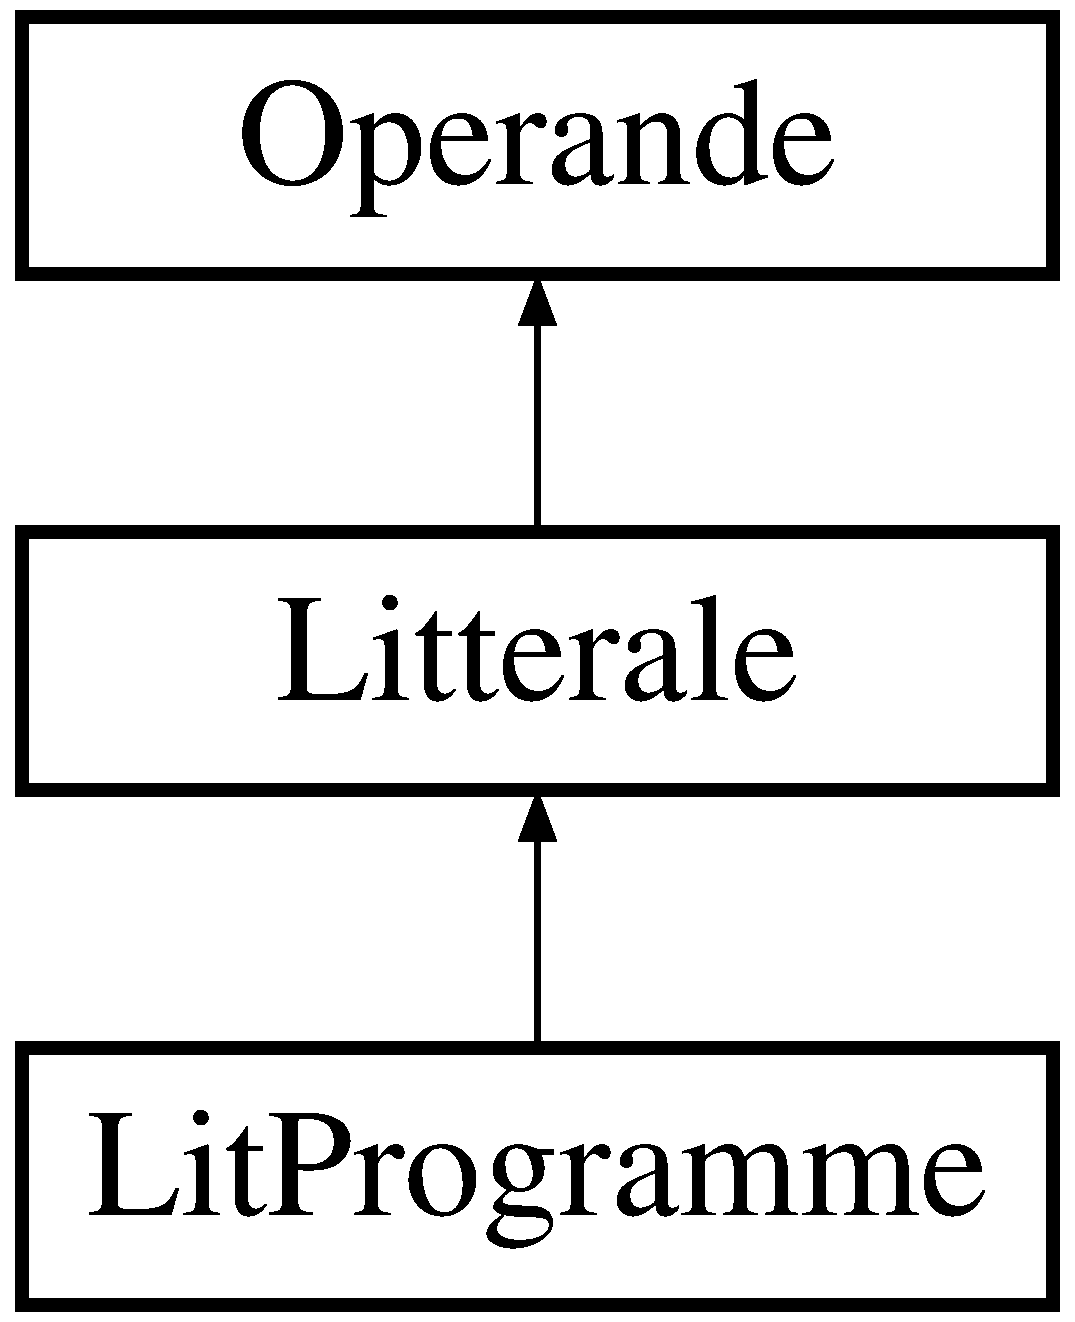
\includegraphics[height=3.000000cm]{class_lit_programme}
\end{center}
\end{figure}
\subsection*{Public Member Functions}
\begin{DoxyCompactItemize}
\item 
\hyperlink{class_lit_programme_aaafb933f7483a4a5020970c9c7e9469a}{Lit\+Programme} (const Q\+String \&str, const Q\+String na=\char`\"{}\char`\"{})
\item 
unsigned int \hyperlink{class_lit_programme_ab17a5bb2c1d595d262115055fef828bf}{get\+Taille} ()
\item 
Q\+String \hyperlink{class_lit_programme_aa95b51a0885edb825b5753d592af024f}{getelem} ()
\item 
Q\+String \hyperlink{class_lit_programme_a8a1086c6458e02378f66144fe1f841be}{to\+String} () const 
\item 
const Q\+String \& \hyperlink{class_lit_programme_a290d6872bcc72ed8c820d198038cb4af}{get\+Value\+Prog} () const 
\end{DoxyCompactItemize}
\subsection*{Additional Inherited Members}


\subsection{Detailed Description}


Definition at line 48 of file litterale.\+h.



\subsection{Constructor \& Destructor Documentation}
\index{Lit\+Programme@{Lit\+Programme}!Lit\+Programme@{Lit\+Programme}}
\index{Lit\+Programme@{Lit\+Programme}!Lit\+Programme@{Lit\+Programme}}
\subsubsection[{\texorpdfstring{Lit\+Programme(const Q\+String \&str, const Q\+String na="""")}{LitProgramme(const QString &str, const QString na="")}}]{\setlength{\rightskip}{0pt plus 5cm}Lit\+Programme\+::\+Lit\+Programme (
\begin{DoxyParamCaption}
\item[{const Q\+String \&}]{str, }
\item[{const Q\+String}]{na = {\ttfamily \char`\"{}\char`\"{}}}
\end{DoxyParamCaption}
)}\hypertarget{class_lit_programme_aaafb933f7483a4a5020970c9c7e9469a}{}\label{class_lit_programme_aaafb933f7483a4a5020970c9c7e9469a}


Definition at line 13 of file litterale.\+cpp.



\subsection{Member Function Documentation}
\index{Lit\+Programme@{Lit\+Programme}!getelem@{getelem}}
\index{getelem@{getelem}!Lit\+Programme@{Lit\+Programme}}
\subsubsection[{\texorpdfstring{getelem()}{getelem()}}]{\setlength{\rightskip}{0pt plus 5cm}Q\+String Lit\+Programme\+::getelem (
\begin{DoxyParamCaption}
{}
\end{DoxyParamCaption}
)\hspace{0.3cm}{\ttfamily [inline]}}\hypertarget{class_lit_programme_aa95b51a0885edb825b5753d592af024f}{}\label{class_lit_programme_aa95b51a0885edb825b5753d592af024f}


Definition at line 55 of file litterale.\+h.

\index{Lit\+Programme@{Lit\+Programme}!get\+Taille@{get\+Taille}}
\index{get\+Taille@{get\+Taille}!Lit\+Programme@{Lit\+Programme}}
\subsubsection[{\texorpdfstring{get\+Taille()}{getTaille()}}]{\setlength{\rightskip}{0pt plus 5cm}unsigned int Lit\+Programme\+::get\+Taille (
\begin{DoxyParamCaption}
{}
\end{DoxyParamCaption}
)\hspace{0.3cm}{\ttfamily [inline]}}\hypertarget{class_lit_programme_ab17a5bb2c1d595d262115055fef828bf}{}\label{class_lit_programme_ab17a5bb2c1d595d262115055fef828bf}


Definition at line 54 of file litterale.\+h.

\index{Lit\+Programme@{Lit\+Programme}!get\+Value\+Prog@{get\+Value\+Prog}}
\index{get\+Value\+Prog@{get\+Value\+Prog}!Lit\+Programme@{Lit\+Programme}}
\subsubsection[{\texorpdfstring{get\+Value\+Prog() const }{getValueProg() const }}]{\setlength{\rightskip}{0pt plus 5cm}const Q\+String\& Lit\+Programme\+::get\+Value\+Prog (
\begin{DoxyParamCaption}
{}
\end{DoxyParamCaption}
) const\hspace{0.3cm}{\ttfamily [inline]}}\hypertarget{class_lit_programme_a290d6872bcc72ed8c820d198038cb4af}{}\label{class_lit_programme_a290d6872bcc72ed8c820d198038cb4af}


Definition at line 57 of file litterale.\+h.

\index{Lit\+Programme@{Lit\+Programme}!to\+String@{to\+String}}
\index{to\+String@{to\+String}!Lit\+Programme@{Lit\+Programme}}
\subsubsection[{\texorpdfstring{to\+String() const }{toString() const }}]{\setlength{\rightskip}{0pt plus 5cm}Q\+String Lit\+Programme\+::to\+String (
\begin{DoxyParamCaption}
{}
\end{DoxyParamCaption}
) const\hspace{0.3cm}{\ttfamily [virtual]}}\hypertarget{class_lit_programme_a8a1086c6458e02378f66144fe1f841be}{}\label{class_lit_programme_a8a1086c6458e02378f66144fe1f841be}


Implements \hyperlink{class_litterale_a3b427621132af2903259390143d1b16d}{Litterale}.



Definition at line 30 of file litterale.\+cpp.



The documentation for this class was generated from the following files\+:\begin{DoxyCompactItemize}
\item 
\hyperlink{litterale_8h}{litterale.\+h}\item 
\hyperlink{litterale_8cpp}{litterale.\+cpp}\end{DoxyCompactItemize}

\hypertarget{class_litterale}{}\section{Litterale Class Reference}
\label{class_litterale}\index{Litterale@{Litterale}}


{\ttfamily \#include $<$litterale.\+h$>$}

Inheritance diagram for Litterale\+:\begin{figure}[H]
\begin{center}
\leavevmode
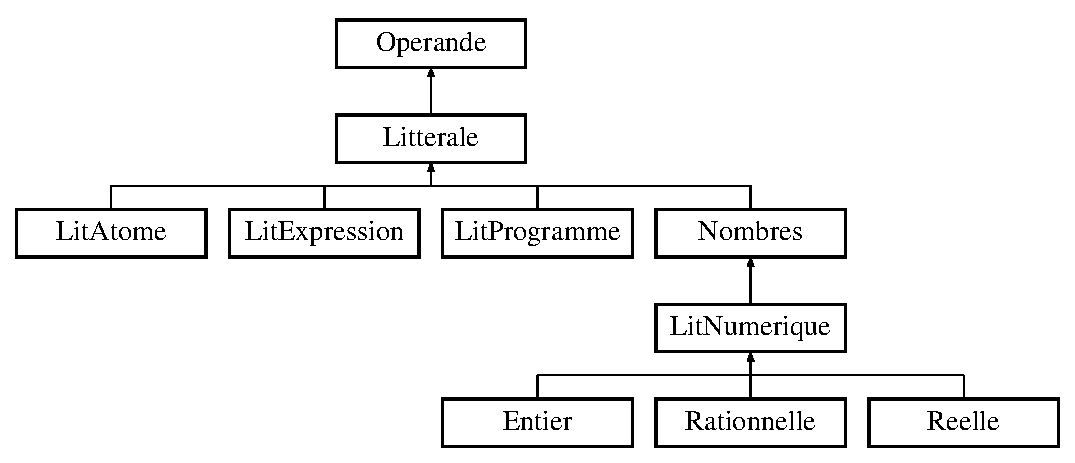
\includegraphics[height=5.000000cm]{class_litterale}
\end{center}
\end{figure}
\subsection*{Public Member Functions}
\begin{DoxyCompactItemize}
\item 
\hyperlink{class_litterale_acb86136fe5bd79b5711c4e64cc1e6284}{Litterale} (const Q\+String \&na=\char`\"{}\char`\"{})
\item 
virtual \hyperlink{class_litterale_af4260da555bb5fe3a24b7f3ad8562ba0}{$\sim$\+Litterale} ()
\item 
virtual Q\+String \hyperlink{class_litterale_a3b427621132af2903259390143d1b16d}{to\+String} () const  =0
\item 
void \hyperlink{class_litterale_a443b6ad424c61d9ce15f9471fcb78c62}{set\+Name} (const Q\+String \&na)
\item 
void \hyperlink{class_litterale_a357f16f4a8c5ed2e06a2441d0a33a27f}{set\+Neg} (bool s)
\item 
bool \hyperlink{class_litterale_a23b71dce3c0635be4e361a950d367329}{get\+Neg} () const 
\end{DoxyCompactItemize}
\subsection*{Protected Attributes}
\begin{DoxyCompactItemize}
\item 
bool \hyperlink{class_litterale_a2477aeadea6c34dce5614e5e8aa701f2}{neg}
\end{DoxyCompactItemize}
\subsection*{Friends}
\begin{DoxyCompactItemize}
\item 
class \hyperlink{class_litterale_a0aab3199db1ebeb99e33e66b9cf8e975}{Litterale\+Manager}
\end{DoxyCompactItemize}


\subsection{Detailed Description}


Definition at line 30 of file litterale.\+h.



\subsection{Constructor \& Destructor Documentation}
\index{Litterale@{Litterale}!Litterale@{Litterale}}
\index{Litterale@{Litterale}!Litterale@{Litterale}}
\subsubsection[{\texorpdfstring{Litterale(const Q\+String \&na="""")}{Litterale(const QString &na="")}}]{\setlength{\rightskip}{0pt plus 5cm}Litterale\+::\+Litterale (
\begin{DoxyParamCaption}
\item[{const Q\+String \&}]{na = {\ttfamily \char`\"{}\char`\"{}}}
\end{DoxyParamCaption}
)\hspace{0.3cm}{\ttfamily [inline]}}\hypertarget{class_litterale_acb86136fe5bd79b5711c4e64cc1e6284}{}\label{class_litterale_acb86136fe5bd79b5711c4e64cc1e6284}


Definition at line 36 of file litterale.\+h.

\index{Litterale@{Litterale}!````~Litterale@{$\sim$\+Litterale}}
\index{````~Litterale@{$\sim$\+Litterale}!Litterale@{Litterale}}
\subsubsection[{\texorpdfstring{$\sim$\+Litterale()}{~Litterale()}}]{\setlength{\rightskip}{0pt plus 5cm}Litterale\+::$\sim$\+Litterale (
\begin{DoxyParamCaption}
{}
\end{DoxyParamCaption}
)\hspace{0.3cm}{\ttfamily [virtual]}}\hypertarget{class_litterale_af4260da555bb5fe3a24b7f3ad8562ba0}{}\label{class_litterale_af4260da555bb5fe3a24b7f3ad8562ba0}


Definition at line 8 of file litterale.\+cpp.



\subsection{Member Function Documentation}
\index{Litterale@{Litterale}!get\+Neg@{get\+Neg}}
\index{get\+Neg@{get\+Neg}!Litterale@{Litterale}}
\subsubsection[{\texorpdfstring{get\+Neg() const }{getNeg() const }}]{\setlength{\rightskip}{0pt plus 5cm}bool Litterale\+::get\+Neg (
\begin{DoxyParamCaption}
{}
\end{DoxyParamCaption}
) const\hspace{0.3cm}{\ttfamily [inline]}}\hypertarget{class_litterale_a23b71dce3c0635be4e361a950d367329}{}\label{class_litterale_a23b71dce3c0635be4e361a950d367329}


Definition at line 42 of file litterale.\+h.

\index{Litterale@{Litterale}!set\+Name@{set\+Name}}
\index{set\+Name@{set\+Name}!Litterale@{Litterale}}
\subsubsection[{\texorpdfstring{set\+Name(const Q\+String \&na)}{setName(const QString &na)}}]{\setlength{\rightskip}{0pt plus 5cm}void Litterale\+::set\+Name (
\begin{DoxyParamCaption}
\item[{const Q\+String \&}]{na}
\end{DoxyParamCaption}
)\hspace{0.3cm}{\ttfamily [inline]}}\hypertarget{class_litterale_a443b6ad424c61d9ce15f9471fcb78c62}{}\label{class_litterale_a443b6ad424c61d9ce15f9471fcb78c62}


Definition at line 40 of file litterale.\+h.

\index{Litterale@{Litterale}!set\+Neg@{set\+Neg}}
\index{set\+Neg@{set\+Neg}!Litterale@{Litterale}}
\subsubsection[{\texorpdfstring{set\+Neg(bool s)}{setNeg(bool s)}}]{\setlength{\rightskip}{0pt plus 5cm}void Litterale\+::set\+Neg (
\begin{DoxyParamCaption}
\item[{bool}]{s}
\end{DoxyParamCaption}
)\hspace{0.3cm}{\ttfamily [inline]}}\hypertarget{class_litterale_a357f16f4a8c5ed2e06a2441d0a33a27f}{}\label{class_litterale_a357f16f4a8c5ed2e06a2441d0a33a27f}


Definition at line 41 of file litterale.\+h.

\index{Litterale@{Litterale}!to\+String@{to\+String}}
\index{to\+String@{to\+String}!Litterale@{Litterale}}
\subsubsection[{\texorpdfstring{to\+String() const  =0}{toString() const  =0}}]{\setlength{\rightskip}{0pt plus 5cm}virtual Q\+String Litterale\+::to\+String (
\begin{DoxyParamCaption}
{}
\end{DoxyParamCaption}
) const\hspace{0.3cm}{\ttfamily [pure virtual]}}\hypertarget{class_litterale_a3b427621132af2903259390143d1b16d}{}\label{class_litterale_a3b427621132af2903259390143d1b16d}


Implements \hyperlink{class_operande_a2acae8f59199e93850b3fdb13eba1672}{Operande}.



Implemented in \hyperlink{class_reelle_add2eb8eb352c8bef1e5d51119b54bcb6}{Reelle}, \hyperlink{class_rationnelle_a406d82b3db71b5d7cac720a12e756c3c}{Rationnelle}, \hyperlink{class_entier_aa960356dfeae8af6dfa2cd25136a1a6f}{Entier}, \hyperlink{class_lit_numerique_a6e3c66f0b484c5be954eb788a95c0d16}{Lit\+Numerique}, \hyperlink{class_nombres_a456e2e58403e79cabdfefb14fd19b4f1}{Nombres}, \hyperlink{class_lit_atome_abbe47368e149ae5a9744bc7188df1cc8}{Lit\+Atome}, \hyperlink{class_lit_expression_a108f8809e4ca49343426c9d0c30c28c4}{Lit\+Expression}, and \hyperlink{class_lit_programme_a8a1086c6458e02378f66144fe1f841be}{Lit\+Programme}.



\subsection{Friends And Related Function Documentation}
\index{Litterale@{Litterale}!Litterale\+Manager@{Litterale\+Manager}}
\index{Litterale\+Manager@{Litterale\+Manager}!Litterale@{Litterale}}
\subsubsection[{\texorpdfstring{Litterale\+Manager}{LitteraleManager}}]{\setlength{\rightskip}{0pt plus 5cm}friend class {\bf Litterale\+Manager}\hspace{0.3cm}{\ttfamily [friend]}}\hypertarget{class_litterale_a0aab3199db1ebeb99e33e66b9cf8e975}{}\label{class_litterale_a0aab3199db1ebeb99e33e66b9cf8e975}


Definition at line 34 of file litterale.\+h.



\subsection{Member Data Documentation}
\index{Litterale@{Litterale}!neg@{neg}}
\index{neg@{neg}!Litterale@{Litterale}}
\subsubsection[{\texorpdfstring{neg}{neg}}]{\setlength{\rightskip}{0pt plus 5cm}bool Litterale\+::neg\hspace{0.3cm}{\ttfamily [protected]}}\hypertarget{class_litterale_a2477aeadea6c34dce5614e5e8aa701f2}{}\label{class_litterale_a2477aeadea6c34dce5614e5e8aa701f2}


Definition at line 33 of file litterale.\+h.



The documentation for this class was generated from the following files\+:\begin{DoxyCompactItemize}
\item 
\hyperlink{litterale_8h}{litterale.\+h}\item 
\hyperlink{litterale_8cpp}{litterale.\+cpp}\end{DoxyCompactItemize}

\hypertarget{class_litterale_manager}{}\section{Litterale\+Manager Class Reference}
\label{class_litterale_manager}\index{Litterale\+Manager@{Litterale\+Manager}}


{\ttfamily \#include $<$computer.\+h$>$}

\subsection*{Classes}
\begin{DoxyCompactItemize}
\item 
class \hyperlink{class_litterale_manager_1_1const__iterator}{const\+\_\+iterator}
\item 
class \hyperlink{class_litterale_manager_1_1iterator}{iterator}
\end{DoxyCompactItemize}
\subsection*{Public Member Functions}
\begin{DoxyCompactItemize}
\item 
bool \hyperlink{class_litterale_manager_ab6a5158f0a5a94d79744188ae9540fc9}{get\+Verif} ()
\item 
void \hyperlink{class_litterale_manager_a4b1068f038f88ccd13fc78b18d979d14}{set\+Verif} (bool v)
\item 
\hyperlink{class_litterale}{Litterale} $\ast$ \hyperlink{class_litterale_manager_aba80b29edd7b1c69cd8cf3d925190523}{add\+Litterale} (const Q\+String \&str)
\item 
\hyperlink{class_litterale}{Litterale} \& \hyperlink{class_litterale_manager_a15a4544d62ce9c19f69a48f152fee97a}{add\+Litterale} (\hyperlink{class_litterale}{Litterale} $\ast$res)
\item 
\hyperlink{class_litterale}{Litterale} $\ast$ \hyperlink{class_litterale_manager_aa1bda888af4e7891092f2c4f38cda6d1}{is\+Rationnelle} (const Q\+String \&c)
\item 
bool \hyperlink{class_litterale_manager_a2430ede43517c01686653397644677a1}{verif\+Litterale} (Q\+String \&op, Q\+String \&nouvelle, Q\+Vector$<$ \hyperlink{class_operande}{Operande} $\ast$ $>$ \&vector\+Exp)
\item 
Q\+String \hyperlink{class_litterale_manager_a755bbf36636b2ad3ebb8590efdd60566}{verif\+Expression\+Valide} (const Q\+String \&c, Q\+Vector$<$ \hyperlink{class_operande}{Operande} $\ast$ $>$ \&vect)
\item 
\hyperlink{class_litterale}{Litterale} $\ast$ \hyperlink{class_litterale_manager_a8be64db76a4365bd5b287c7ed5c87ca3}{fabriq\+Litterale} (const Q\+String \&v)
\item 
void \hyperlink{class_litterale_manager_a02ac5f4d721e6cb2154c26e589e79076}{remove\+Litterale} (\hyperlink{class_litterale}{Litterale} \&e)
\item 
Q\+String \hyperlink{class_litterale_manager_a1c0db3db1e3f62e480f0717b8c10b79f}{message\+Nouvelle\+Creation} (\hyperlink{class_litterale}{Litterale} \&lit)
\item 
\hyperlink{class_litterale_manager_1_1iterator}{iterator} \hyperlink{class_litterale_manager_a4797bac6083540c62424efebba3d3b82}{begin} ()
\item 
\hyperlink{class_litterale_manager_1_1iterator}{iterator} \hyperlink{class_litterale_manager_a89555cde8edcae47c1cb682a51be5880}{end} ()
\item 
\hyperlink{class_litterale_manager_1_1const__iterator}{const\+\_\+iterator} \hyperlink{class_litterale_manager_addd9a9a3b5d5846cd4e4e88881c48821}{begin} () const 
\item 
\hyperlink{class_litterale_manager_1_1const__iterator}{const\+\_\+iterator} \hyperlink{class_litterale_manager_aa3b3319b0d2a657d1a894ec07869c2a1}{end} () const 
\end{DoxyCompactItemize}
\subsection*{Static Public Member Functions}
\begin{DoxyCompactItemize}
\item 
static \hyperlink{class_litterale_manager}{Litterale\+Manager} \& \hyperlink{class_litterale_manager_ac8d443e8cfb074539064d2e02ef95416}{get\+Instance} ()
\item 
static void \hyperlink{class_litterale_manager_a9b97f46ce105dcaf3128745a6e1f239c}{liberer\+Instance} ()
\end{DoxyCompactItemize}


\subsection{Detailed Description}


Definition at line 13 of file computer.\+h.



\subsection{Member Function Documentation}
\index{Litterale\+Manager@{Litterale\+Manager}!add\+Litterale@{add\+Litterale}}
\index{add\+Litterale@{add\+Litterale}!Litterale\+Manager@{Litterale\+Manager}}
\subsubsection[{\texorpdfstring{add\+Litterale(const Q\+String \&str)}{addLitterale(const QString &str)}}]{\setlength{\rightskip}{0pt plus 5cm}{\bf Litterale} $\ast$ Litterale\+Manager\+::add\+Litterale (
\begin{DoxyParamCaption}
\item[{const Q\+String \&}]{str}
\end{DoxyParamCaption}
)}\hypertarget{class_litterale_manager_aba80b29edd7b1c69cd8cf3d925190523}{}\label{class_litterale_manager_aba80b29edd7b1c69cd8cf3d925190523}


Definition at line 178 of file computer.\+cpp.

\index{Litterale\+Manager@{Litterale\+Manager}!add\+Litterale@{add\+Litterale}}
\index{add\+Litterale@{add\+Litterale}!Litterale\+Manager@{Litterale\+Manager}}
\subsubsection[{\texorpdfstring{add\+Litterale(\+Litterale $\ast$res)}{addLitterale(Litterale *res)}}]{\setlength{\rightskip}{0pt plus 5cm}{\bf Litterale} \& Litterale\+Manager\+::add\+Litterale (
\begin{DoxyParamCaption}
\item[{{\bf Litterale} $\ast$}]{res}
\end{DoxyParamCaption}
)}\hypertarget{class_litterale_manager_a15a4544d62ce9c19f69a48f152fee97a}{}\label{class_litterale_manager_a15a4544d62ce9c19f69a48f152fee97a}


Definition at line 188 of file computer.\+cpp.

\index{Litterale\+Manager@{Litterale\+Manager}!begin@{begin}}
\index{begin@{begin}!Litterale\+Manager@{Litterale\+Manager}}
\subsubsection[{\texorpdfstring{begin()}{begin()}}]{\setlength{\rightskip}{0pt plus 5cm}{\bf iterator} Litterale\+Manager\+::begin (
\begin{DoxyParamCaption}
{}
\end{DoxyParamCaption}
)\hspace{0.3cm}{\ttfamily [inline]}}\hypertarget{class_litterale_manager_a4797bac6083540c62424efebba3d3b82}{}\label{class_litterale_manager_a4797bac6083540c62424efebba3d3b82}


Definition at line 54 of file computer.\+h.

\index{Litterale\+Manager@{Litterale\+Manager}!begin@{begin}}
\index{begin@{begin}!Litterale\+Manager@{Litterale\+Manager}}
\subsubsection[{\texorpdfstring{begin() const }{begin() const }}]{\setlength{\rightskip}{0pt plus 5cm}{\bf const\+\_\+iterator} Litterale\+Manager\+::begin (
\begin{DoxyParamCaption}
{}
\end{DoxyParamCaption}
) const\hspace{0.3cm}{\ttfamily [inline]}}\hypertarget{class_litterale_manager_addd9a9a3b5d5846cd4e4e88881c48821}{}\label{class_litterale_manager_addd9a9a3b5d5846cd4e4e88881c48821}


Definition at line 67 of file computer.\+h.

\index{Litterale\+Manager@{Litterale\+Manager}!end@{end}}
\index{end@{end}!Litterale\+Manager@{Litterale\+Manager}}
\subsubsection[{\texorpdfstring{end()}{end()}}]{\setlength{\rightskip}{0pt plus 5cm}{\bf iterator} Litterale\+Manager\+::end (
\begin{DoxyParamCaption}
{}
\end{DoxyParamCaption}
)\hspace{0.3cm}{\ttfamily [inline]}}\hypertarget{class_litterale_manager_a89555cde8edcae47c1cb682a51be5880}{}\label{class_litterale_manager_a89555cde8edcae47c1cb682a51be5880}


Definition at line 55 of file computer.\+h.

\index{Litterale\+Manager@{Litterale\+Manager}!end@{end}}
\index{end@{end}!Litterale\+Manager@{Litterale\+Manager}}
\subsubsection[{\texorpdfstring{end() const }{end() const }}]{\setlength{\rightskip}{0pt plus 5cm}{\bf const\+\_\+iterator} Litterale\+Manager\+::end (
\begin{DoxyParamCaption}
{}
\end{DoxyParamCaption}
) const\hspace{0.3cm}{\ttfamily [inline]}}\hypertarget{class_litterale_manager_aa3b3319b0d2a657d1a894ec07869c2a1}{}\label{class_litterale_manager_aa3b3319b0d2a657d1a894ec07869c2a1}


Definition at line 68 of file computer.\+h.

\index{Litterale\+Manager@{Litterale\+Manager}!fabriq\+Litterale@{fabriq\+Litterale}}
\index{fabriq\+Litterale@{fabriq\+Litterale}!Litterale\+Manager@{Litterale\+Manager}}
\subsubsection[{\texorpdfstring{fabriq\+Litterale(const Q\+String \&v)}{fabriqLitterale(const QString &v)}}]{\setlength{\rightskip}{0pt plus 5cm}{\bf Litterale} $\ast$ Litterale\+Manager\+::fabriq\+Litterale (
\begin{DoxyParamCaption}
\item[{const Q\+String \&}]{v}
\end{DoxyParamCaption}
)}\hypertarget{class_litterale_manager_a8be64db76a4365bd5b287c7ed5c87ca3}{}\label{class_litterale_manager_a8be64db76a4365bd5b287c7ed5c87ca3}


Definition at line 140 of file computer.\+cpp.

\index{Litterale\+Manager@{Litterale\+Manager}!get\+Instance@{get\+Instance}}
\index{get\+Instance@{get\+Instance}!Litterale\+Manager@{Litterale\+Manager}}
\subsubsection[{\texorpdfstring{get\+Instance()}{getInstance()}}]{\setlength{\rightskip}{0pt plus 5cm}{\bf Litterale\+Manager} \& Litterale\+Manager\+::get\+Instance (
\begin{DoxyParamCaption}
{}
\end{DoxyParamCaption}
)\hspace{0.3cm}{\ttfamily [static]}}\hypertarget{class_litterale_manager_ac8d443e8cfb074539064d2e02ef95416}{}\label{class_litterale_manager_ac8d443e8cfb074539064d2e02ef95416}


Definition at line 7 of file computer.\+cpp.

\index{Litterale\+Manager@{Litterale\+Manager}!get\+Verif@{get\+Verif}}
\index{get\+Verif@{get\+Verif}!Litterale\+Manager@{Litterale\+Manager}}
\subsubsection[{\texorpdfstring{get\+Verif()}{getVerif()}}]{\setlength{\rightskip}{0pt plus 5cm}bool Litterale\+Manager\+::get\+Verif (
\begin{DoxyParamCaption}
{}
\end{DoxyParamCaption}
)\hspace{0.3cm}{\ttfamily [inline]}}\hypertarget{class_litterale_manager_ab6a5158f0a5a94d79744188ae9540fc9}{}\label{class_litterale_manager_ab6a5158f0a5a94d79744188ae9540fc9}


Definition at line 32 of file computer.\+h.

\index{Litterale\+Manager@{Litterale\+Manager}!is\+Rationnelle@{is\+Rationnelle}}
\index{is\+Rationnelle@{is\+Rationnelle}!Litterale\+Manager@{Litterale\+Manager}}
\subsubsection[{\texorpdfstring{is\+Rationnelle(const Q\+String \&c)}{isRationnelle(const QString &c)}}]{\setlength{\rightskip}{0pt plus 5cm}{\bf Litterale} $\ast$ Litterale\+Manager\+::is\+Rationnelle (
\begin{DoxyParamCaption}
\item[{const Q\+String \&}]{c}
\end{DoxyParamCaption}
)}\hypertarget{class_litterale_manager_aa1bda888af4e7891092f2c4f38cda6d1}{}\label{class_litterale_manager_aa1bda888af4e7891092f2c4f38cda6d1}


Definition at line 27 of file computer.\+cpp.

\index{Litterale\+Manager@{Litterale\+Manager}!liberer\+Instance@{liberer\+Instance}}
\index{liberer\+Instance@{liberer\+Instance}!Litterale\+Manager@{Litterale\+Manager}}
\subsubsection[{\texorpdfstring{liberer\+Instance()}{libererInstance()}}]{\setlength{\rightskip}{0pt plus 5cm}void Litterale\+Manager\+::liberer\+Instance (
\begin{DoxyParamCaption}
{}
\end{DoxyParamCaption}
)\hspace{0.3cm}{\ttfamily [static]}}\hypertarget{class_litterale_manager_a9b97f46ce105dcaf3128745a6e1f239c}{}\label{class_litterale_manager_a9b97f46ce105dcaf3128745a6e1f239c}


Definition at line 12 of file computer.\+cpp.

\index{Litterale\+Manager@{Litterale\+Manager}!message\+Nouvelle\+Creation@{message\+Nouvelle\+Creation}}
\index{message\+Nouvelle\+Creation@{message\+Nouvelle\+Creation}!Litterale\+Manager@{Litterale\+Manager}}
\subsubsection[{\texorpdfstring{message\+Nouvelle\+Creation(\+Litterale \&lit)}{messageNouvelleCreation(Litterale &lit)}}]{\setlength{\rightskip}{0pt plus 5cm}Q\+String Litterale\+Manager\+::message\+Nouvelle\+Creation (
\begin{DoxyParamCaption}
\item[{{\bf Litterale} \&}]{lit}
\end{DoxyParamCaption}
)}\hypertarget{class_litterale_manager_a1c0db3db1e3f62e480f0717b8c10b79f}{}\label{class_litterale_manager_a1c0db3db1e3f62e480f0717b8c10b79f}


Definition at line 216 of file computer.\+cpp.

\index{Litterale\+Manager@{Litterale\+Manager}!remove\+Litterale@{remove\+Litterale}}
\index{remove\+Litterale@{remove\+Litterale}!Litterale\+Manager@{Litterale\+Manager}}
\subsubsection[{\texorpdfstring{remove\+Litterale(\+Litterale \&e)}{removeLitterale(Litterale &e)}}]{\setlength{\rightskip}{0pt plus 5cm}void Litterale\+Manager\+::remove\+Litterale (
\begin{DoxyParamCaption}
\item[{{\bf Litterale} \&}]{e}
\end{DoxyParamCaption}
)}\hypertarget{class_litterale_manager_a02ac5f4d721e6cb2154c26e589e79076}{}\label{class_litterale_manager_a02ac5f4d721e6cb2154c26e589e79076}


Definition at line 195 of file computer.\+cpp.

\index{Litterale\+Manager@{Litterale\+Manager}!set\+Verif@{set\+Verif}}
\index{set\+Verif@{set\+Verif}!Litterale\+Manager@{Litterale\+Manager}}
\subsubsection[{\texorpdfstring{set\+Verif(bool v)}{setVerif(bool v)}}]{\setlength{\rightskip}{0pt plus 5cm}void Litterale\+Manager\+::set\+Verif (
\begin{DoxyParamCaption}
\item[{bool}]{v}
\end{DoxyParamCaption}
)\hspace{0.3cm}{\ttfamily [inline]}}\hypertarget{class_litterale_manager_a4b1068f038f88ccd13fc78b18d979d14}{}\label{class_litterale_manager_a4b1068f038f88ccd13fc78b18d979d14}


Definition at line 33 of file computer.\+h.

\index{Litterale\+Manager@{Litterale\+Manager}!verif\+Expression\+Valide@{verif\+Expression\+Valide}}
\index{verif\+Expression\+Valide@{verif\+Expression\+Valide}!Litterale\+Manager@{Litterale\+Manager}}
\subsubsection[{\texorpdfstring{verif\+Expression\+Valide(const Q\+String \&c, Q\+Vector$<$ Operande $\ast$ $>$ \&vect)}{verifExpressionValide(const QString &c, QVector< Operande * > &vect)}}]{\setlength{\rightskip}{0pt plus 5cm}Q\+String Litterale\+Manager\+::verif\+Expression\+Valide (
\begin{DoxyParamCaption}
\item[{const Q\+String \&}]{c, }
\item[{Q\+Vector$<$ {\bf Operande} $\ast$ $>$ \&}]{vect}
\end{DoxyParamCaption}
)}\hypertarget{class_litterale_manager_a755bbf36636b2ad3ebb8590efdd60566}{}\label{class_litterale_manager_a755bbf36636b2ad3ebb8590efdd60566}


Definition at line 82 of file computer.\+cpp.

\index{Litterale\+Manager@{Litterale\+Manager}!verif\+Litterale@{verif\+Litterale}}
\index{verif\+Litterale@{verif\+Litterale}!Litterale\+Manager@{Litterale\+Manager}}
\subsubsection[{\texorpdfstring{verif\+Litterale(\+Q\+String \&op, Q\+String \&nouvelle, Q\+Vector$<$ Operande $\ast$ $>$ \&vector\+Exp)}{verifLitterale(QString &op, QString &nouvelle, QVector< Operande * > &vectorExp)}}]{\setlength{\rightskip}{0pt plus 5cm}bool Litterale\+Manager\+::verif\+Litterale (
\begin{DoxyParamCaption}
\item[{Q\+String \&}]{op, }
\item[{Q\+String \&}]{nouvelle, }
\item[{Q\+Vector$<$ {\bf Operande} $\ast$ $>$ \&}]{vector\+Exp}
\end{DoxyParamCaption}
)}\hypertarget{class_litterale_manager_a2430ede43517c01686653397644677a1}{}\label{class_litterale_manager_a2430ede43517c01686653397644677a1}


Definition at line 59 of file computer.\+cpp.



The documentation for this class was generated from the following files\+:\begin{DoxyCompactItemize}
\item 
\hyperlink{computer_8h}{computer.\+h}\item 
\hyperlink{computer_8cpp}{computer.\+cpp}\end{DoxyCompactItemize}

\hypertarget{class_nombres}{}\section{Nombres Class Reference}
\label{class_nombres}\index{Nombres@{Nombres}}


{\ttfamily \#include $<$litterale.\+h$>$}

Inheritance diagram for Nombres\+:\begin{figure}[H]
\begin{center}
\leavevmode
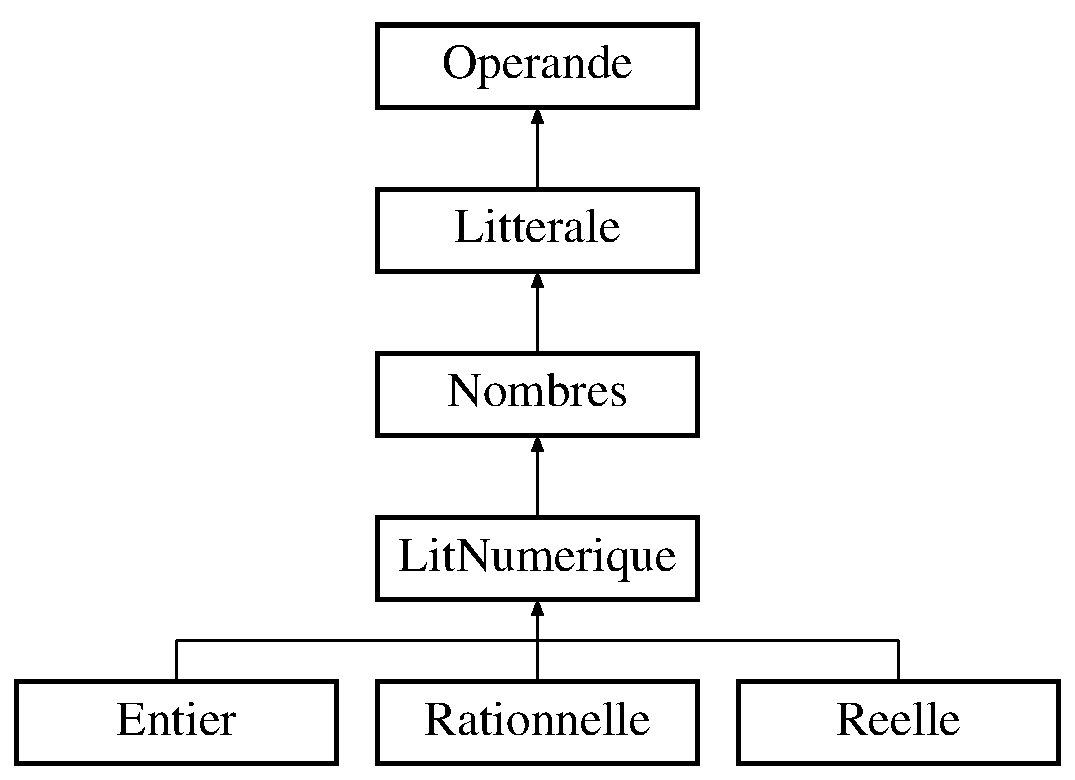
\includegraphics[height=5.000000cm]{class_nombres}
\end{center}
\end{figure}
\subsection*{Public Member Functions}
\begin{DoxyCompactItemize}
\item 
\hyperlink{class_nombres_aa704174b95cbac83fdb4f7ebef8c7e61}{Nombres} (const Q\+String \&na=\char`\"{}\char`\"{})
\item 
virtual \hyperlink{class_nombres_a3477192baa59691c68579251d40bdbcd}{$\sim$\+Nombres} ()
\item 
\hyperlink{class_litterale}{Litterale} $\ast$ \hyperlink{class_nombres_a82cf0b5a3182dcbfbedb75e81ac1e4f0}{return\+Type} ()
\item 
virtual Q\+String \hyperlink{class_nombres_a456e2e58403e79cabdfefb14fd19b4f1}{to\+String} () const  =0
\end{DoxyCompactItemize}
\subsection*{Additional Inherited Members}


\subsection{Detailed Description}


Definition at line 87 of file litterale.\+h.



\subsection{Constructor \& Destructor Documentation}
\index{Nombres@{Nombres}!Nombres@{Nombres}}
\index{Nombres@{Nombres}!Nombres@{Nombres}}
\subsubsection[{\texorpdfstring{Nombres(const Q\+String \&na="""")}{Nombres(const QString &na="")}}]{\setlength{\rightskip}{0pt plus 5cm}Nombres\+::\+Nombres (
\begin{DoxyParamCaption}
\item[{const Q\+String \&}]{na = {\ttfamily \char`\"{}\char`\"{}}}
\end{DoxyParamCaption}
)\hspace{0.3cm}{\ttfamily [inline]}}\hypertarget{class_nombres_aa704174b95cbac83fdb4f7ebef8c7e61}{}\label{class_nombres_aa704174b95cbac83fdb4f7ebef8c7e61}


Definition at line 89 of file litterale.\+h.

\index{Nombres@{Nombres}!````~Nombres@{$\sim$\+Nombres}}
\index{````~Nombres@{$\sim$\+Nombres}!Nombres@{Nombres}}
\subsubsection[{\texorpdfstring{$\sim$\+Nombres()}{~Nombres()}}]{\setlength{\rightskip}{0pt plus 5cm}virtual Nombres\+::$\sim$\+Nombres (
\begin{DoxyParamCaption}
{}
\end{DoxyParamCaption}
)\hspace{0.3cm}{\ttfamily [inline]}, {\ttfamily [virtual]}}\hypertarget{class_nombres_a3477192baa59691c68579251d40bdbcd}{}\label{class_nombres_a3477192baa59691c68579251d40bdbcd}


Definition at line 90 of file litterale.\+h.



\subsection{Member Function Documentation}
\index{Nombres@{Nombres}!return\+Type@{return\+Type}}
\index{return\+Type@{return\+Type}!Nombres@{Nombres}}
\subsubsection[{\texorpdfstring{return\+Type()}{returnType()}}]{\setlength{\rightskip}{0pt plus 5cm}{\bf Litterale} $\ast$ Nombres\+::return\+Type (
\begin{DoxyParamCaption}
{}
\end{DoxyParamCaption}
)}\hypertarget{class_nombres_a82cf0b5a3182dcbfbedb75e81ac1e4f0}{}\label{class_nombres_a82cf0b5a3182dcbfbedb75e81ac1e4f0}


Definition at line 65 of file litterale.\+cpp.

\index{Nombres@{Nombres}!to\+String@{to\+String}}
\index{to\+String@{to\+String}!Nombres@{Nombres}}
\subsubsection[{\texorpdfstring{to\+String() const  =0}{toString() const  =0}}]{\setlength{\rightskip}{0pt plus 5cm}virtual Q\+String Nombres\+::to\+String (
\begin{DoxyParamCaption}
{}
\end{DoxyParamCaption}
) const\hspace{0.3cm}{\ttfamily [pure virtual]}}\hypertarget{class_nombres_a456e2e58403e79cabdfefb14fd19b4f1}{}\label{class_nombres_a456e2e58403e79cabdfefb14fd19b4f1}


Implements \hyperlink{class_litterale_a3b427621132af2903259390143d1b16d}{Litterale}.



Implemented in \hyperlink{class_reelle_add2eb8eb352c8bef1e5d51119b54bcb6}{Reelle}, \hyperlink{class_rationnelle_a406d82b3db71b5d7cac720a12e756c3c}{Rationnelle}, \hyperlink{class_entier_aa960356dfeae8af6dfa2cd25136a1a6f}{Entier}, and \hyperlink{class_lit_numerique_a6e3c66f0b484c5be954eb788a95c0d16}{Lit\+Numerique}.



The documentation for this class was generated from the following files\+:\begin{DoxyCompactItemize}
\item 
\hyperlink{litterale_8h}{litterale.\+h}\item 
\hyperlink{litterale_8cpp}{litterale.\+cpp}\end{DoxyCompactItemize}

\hypertarget{class_op_and}{}\section{Op\+And Class Reference}
\label{class_op_and}\index{Op\+And@{Op\+And}}


{\ttfamily \#include $<$operator\+Logique.\+h$>$}

Inheritance diagram for Op\+And\+:\begin{figure}[H]
\begin{center}
\leavevmode
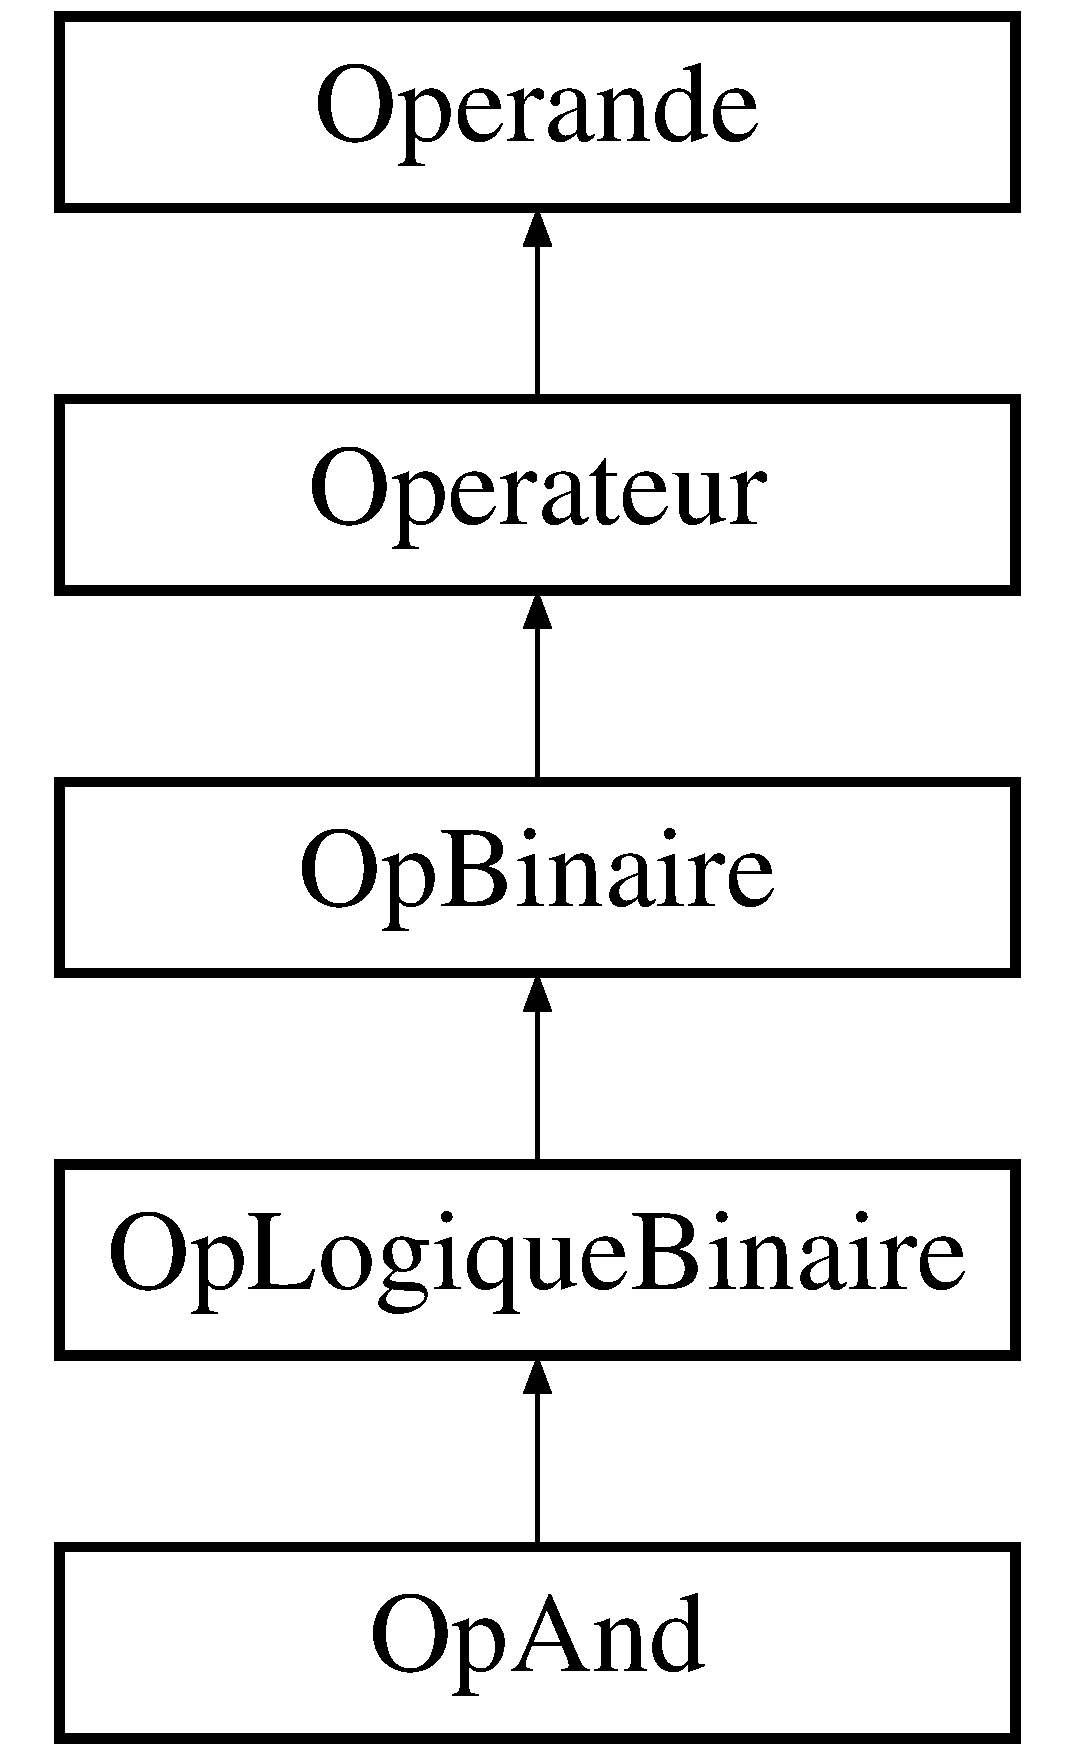
\includegraphics[height=5.000000cm]{class_op_and}
\end{center}
\end{figure}
\subsection*{Public Member Functions}
\begin{DoxyCompactItemize}
\item 
\hyperlink{class_op_and_acc3189423cfa3cb891770e20bd5de7f1}{Op\+And} ()
\item 
\hyperlink{class_litterale}{Litterale} $\ast$ \hyperlink{class_op_and_a84274acf7a0d4e48ff11a9683d488808}{action\+Logi\+Numerique} (\hyperlink{class_lit_numerique}{Lit\+Numerique} $\ast$arg1, \hyperlink{class_lit_numerique}{Lit\+Numerique} $\ast$arg2)
\end{DoxyCompactItemize}
\subsection*{Additional Inherited Members}


\subsection{Detailed Description}


Definition at line 61 of file operator\+Logique.\+h.



\subsection{Constructor \& Destructor Documentation}
\index{Op\+And@{Op\+And}!Op\+And@{Op\+And}}
\index{Op\+And@{Op\+And}!Op\+And@{Op\+And}}
\subsubsection[{\texorpdfstring{Op\+And()}{OpAnd()}}]{\setlength{\rightskip}{0pt plus 5cm}Op\+And\+::\+Op\+And (
\begin{DoxyParamCaption}
{}
\end{DoxyParamCaption}
)\hspace{0.3cm}{\ttfamily [inline]}}\hypertarget{class_op_and_acc3189423cfa3cb891770e20bd5de7f1}{}\label{class_op_and_acc3189423cfa3cb891770e20bd5de7f1}


Definition at line 63 of file operator\+Logique.\+h.



\subsection{Member Function Documentation}
\index{Op\+And@{Op\+And}!action\+Logi\+Numerique@{action\+Logi\+Numerique}}
\index{action\+Logi\+Numerique@{action\+Logi\+Numerique}!Op\+And@{Op\+And}}
\subsubsection[{\texorpdfstring{action\+Logi\+Numerique(\+Lit\+Numerique $\ast$arg1, Lit\+Numerique $\ast$arg2)}{actionLogiNumerique(LitNumerique *arg1, LitNumerique *arg2)}}]{\setlength{\rightskip}{0pt plus 5cm}{\bf Litterale} $\ast$ Op\+And\+::action\+Logi\+Numerique (
\begin{DoxyParamCaption}
\item[{{\bf Lit\+Numerique} $\ast$}]{arg1, }
\item[{{\bf Lit\+Numerique} $\ast$}]{arg2}
\end{DoxyParamCaption}
)\hspace{0.3cm}{\ttfamily [virtual]}}\hypertarget{class_op_and_a84274acf7a0d4e48ff11a9683d488808}{}\label{class_op_and_a84274acf7a0d4e48ff11a9683d488808}


Implements \hyperlink{class_op_logique_binaire_a8fcab4c45ebcadbbcfecfa0c02e36f21}{Op\+Logique\+Binaire}.



Definition at line 56 of file operator\+Logique.\+cpp.



The documentation for this class was generated from the following files\+:\begin{DoxyCompactItemize}
\item 
\hyperlink{operator_logique_8h}{operator\+Logique.\+h}\item 
\hyperlink{operator_logique_8cpp}{operator\+Logique.\+cpp}\end{DoxyCompactItemize}

\hypertarget{class_op_and_factory}{}\section{Op\+And\+Factory Class Reference}
\label{class_op_and_factory}\index{Op\+And\+Factory@{Op\+And\+Factory}}


{\ttfamily \#include $<$operator\+Factory.\+h$>$}

Inheritance diagram for Op\+And\+Factory\+:\begin{figure}[H]
\begin{center}
\leavevmode
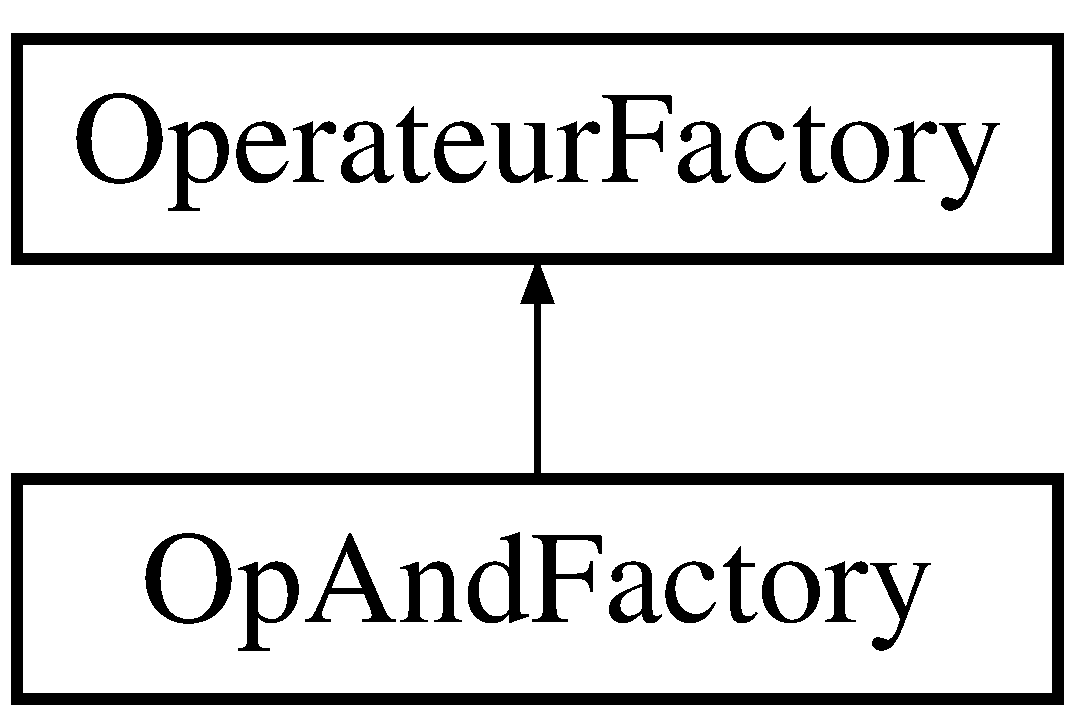
\includegraphics[height=2.000000cm]{class_op_and_factory}
\end{center}
\end{figure}
\subsection*{Public Member Functions}
\begin{DoxyCompactItemize}
\item 
\hyperlink{class_op_and_factory_ae751fb79cb800cfa5cfa94b3624dac75}{Op\+And\+Factory} ()
\item 
\hyperlink{class_operateur}{Operateur} $\ast$ \hyperlink{class_op_and_factory_a7ecd98d30de9c030435385fdeba14566}{get\+Operateur} ()
\end{DoxyCompactItemize}
\subsection*{Additional Inherited Members}


\subsection{Detailed Description}


Definition at line 173 of file operator\+Factory.\+h.



\subsection{Constructor \& Destructor Documentation}
\index{Op\+And\+Factory@{Op\+And\+Factory}!Op\+And\+Factory@{Op\+And\+Factory}}
\index{Op\+And\+Factory@{Op\+And\+Factory}!Op\+And\+Factory@{Op\+And\+Factory}}
\subsubsection[{\texorpdfstring{Op\+And\+Factory()}{OpAndFactory()}}]{\setlength{\rightskip}{0pt plus 5cm}Op\+And\+Factory\+::\+Op\+And\+Factory (
\begin{DoxyParamCaption}
{}
\end{DoxyParamCaption}
)\hspace{0.3cm}{\ttfamily [inline]}}\hypertarget{class_op_and_factory_ae751fb79cb800cfa5cfa94b3624dac75}{}\label{class_op_and_factory_ae751fb79cb800cfa5cfa94b3624dac75}


Definition at line 175 of file operator\+Factory.\+h.



\subsection{Member Function Documentation}
\index{Op\+And\+Factory@{Op\+And\+Factory}!get\+Operateur@{get\+Operateur}}
\index{get\+Operateur@{get\+Operateur}!Op\+And\+Factory@{Op\+And\+Factory}}
\subsubsection[{\texorpdfstring{get\+Operateur()}{getOperateur()}}]{\setlength{\rightskip}{0pt plus 5cm}{\bf Operateur}$\ast$ Op\+And\+Factory\+::get\+Operateur (
\begin{DoxyParamCaption}
{}
\end{DoxyParamCaption}
)\hspace{0.3cm}{\ttfamily [inline]}, {\ttfamily [virtual]}}\hypertarget{class_op_and_factory_a7ecd98d30de9c030435385fdeba14566}{}\label{class_op_and_factory_a7ecd98d30de9c030435385fdeba14566}


Implements \hyperlink{class_operateur_factory_aff61b2f67451f086d6abaea4231b2d78}{Operateur\+Factory}.



Definition at line 176 of file operator\+Factory.\+h.



The documentation for this class was generated from the following file\+:\begin{DoxyCompactItemize}
\item 
\hyperlink{operator_factory_8h}{operator\+Factory.\+h}\end{DoxyCompactItemize}

\hypertarget{class_op_autre}{}\section{Op\+Autre Class Reference}
\label{class_op_autre}\index{Op\+Autre@{Op\+Autre}}


{\ttfamily \#include $<$operator\+Autre.\+h$>$}

Inheritance diagram for Op\+Autre\+:\begin{figure}[H]
\begin{center}
\leavevmode
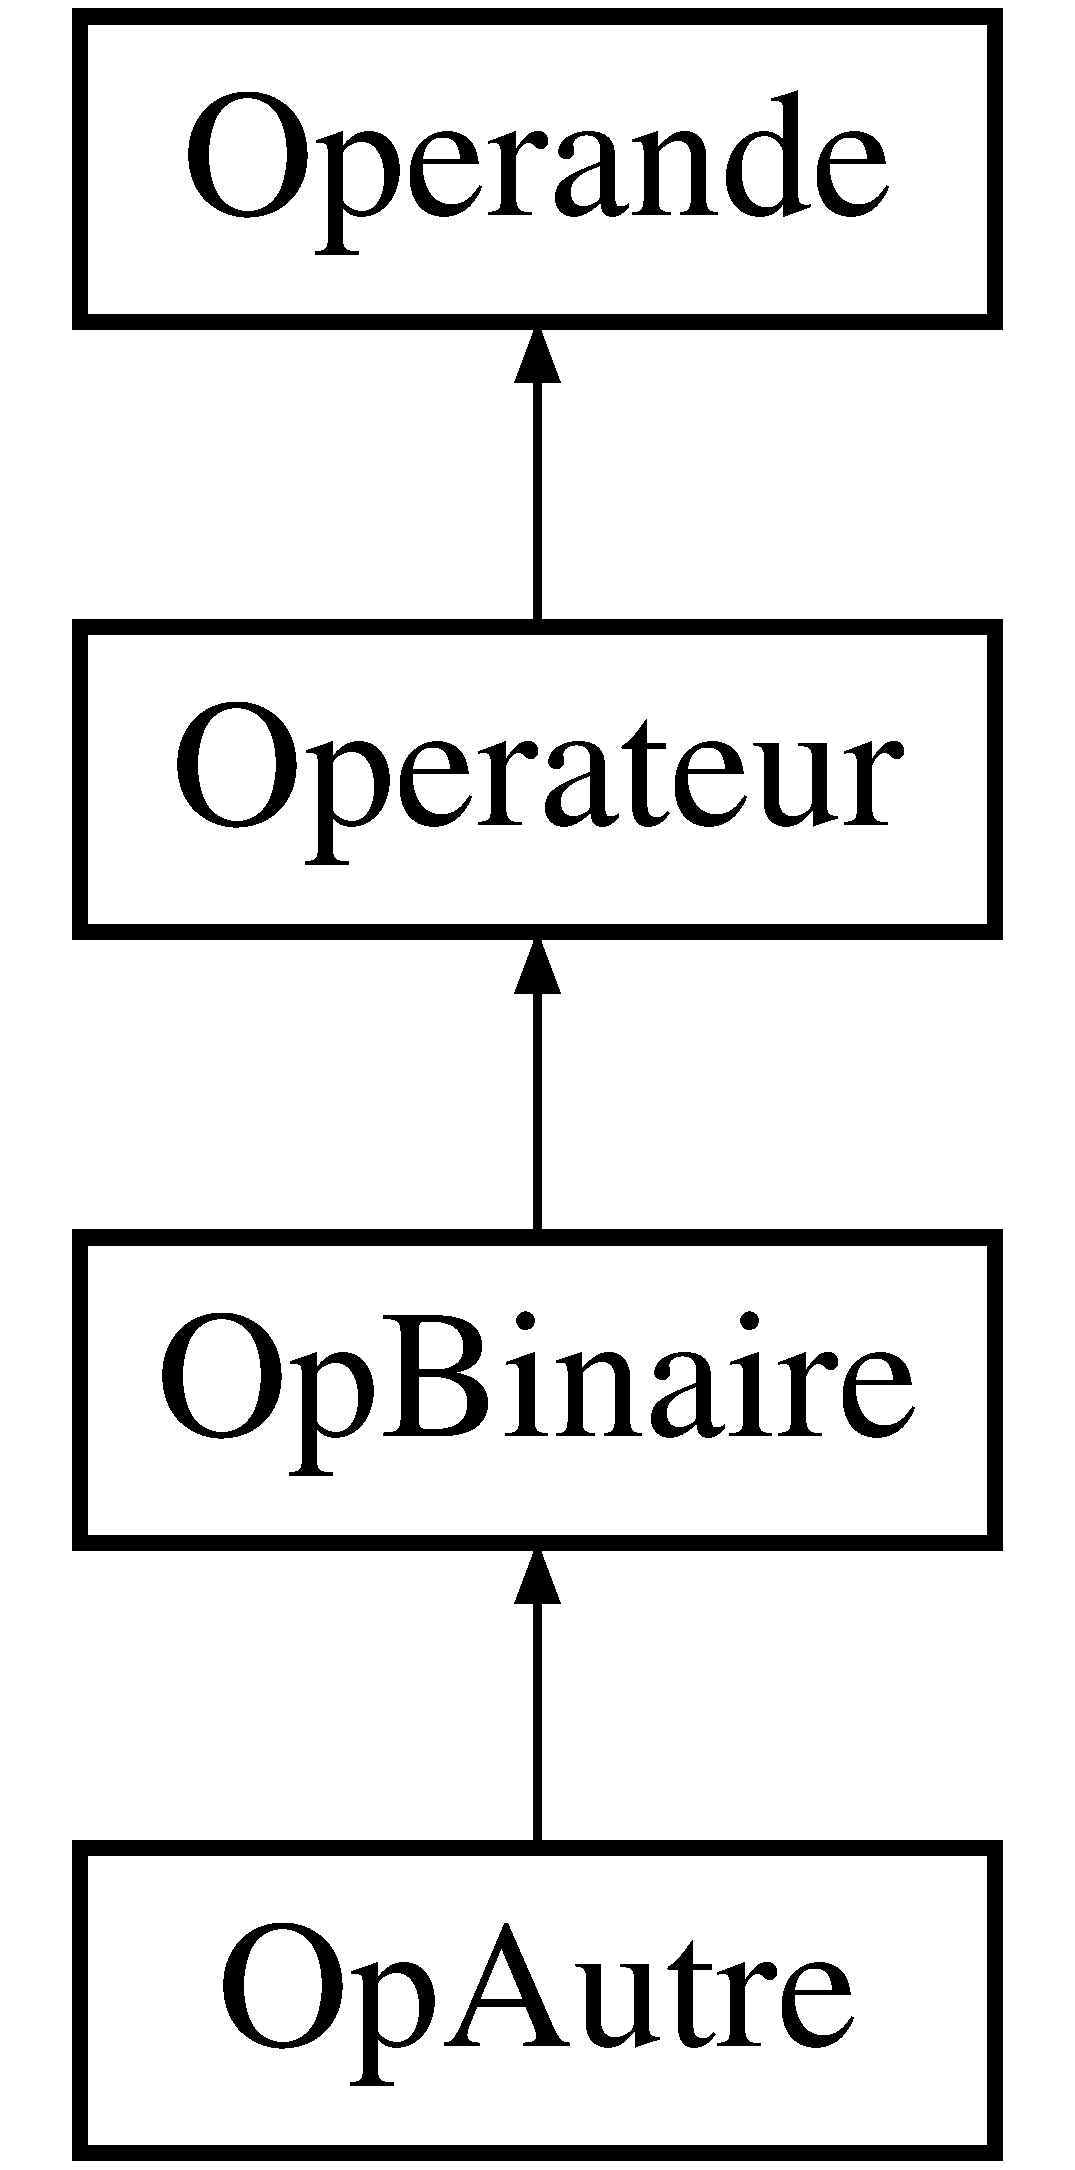
\includegraphics[height=4.000000cm]{class_op_autre}
\end{center}
\end{figure}
\subsection*{Public Member Functions}
\begin{DoxyCompactItemize}
\item 
\hyperlink{class_op_autre_a39a288ba34b8b4537411f73d22e7d0f6}{Op\+Autre} (const Q\+String \&na)
\end{DoxyCompactItemize}
\subsection*{Additional Inherited Members}


\subsection{Detailed Description}


Definition at line 6 of file operator\+Autre.\+h.



\subsection{Constructor \& Destructor Documentation}
\index{Op\+Autre@{Op\+Autre}!Op\+Autre@{Op\+Autre}}
\index{Op\+Autre@{Op\+Autre}!Op\+Autre@{Op\+Autre}}
\subsubsection[{\texorpdfstring{Op\+Autre(const Q\+String \&na)}{OpAutre(const QString &na)}}]{\setlength{\rightskip}{0pt plus 5cm}Op\+Autre\+::\+Op\+Autre (
\begin{DoxyParamCaption}
\item[{const Q\+String \&}]{na}
\end{DoxyParamCaption}
)\hspace{0.3cm}{\ttfamily [inline]}}\hypertarget{class_op_autre_a39a288ba34b8b4537411f73d22e7d0f6}{}\label{class_op_autre_a39a288ba34b8b4537411f73d22e7d0f6}


Definition at line 8 of file operator\+Autre.\+h.



The documentation for this class was generated from the following file\+:\begin{DoxyCompactItemize}
\item 
\hyperlink{operator_autre_8h}{operator\+Autre.\+h}\end{DoxyCompactItemize}

\hypertarget{class_op_binaire}{}\section{Op\+Binaire Class Reference}
\label{class_op_binaire}\index{Op\+Binaire@{Op\+Binaire}}


{\ttfamily \#include $<$operator.\+h$>$}

Inheritance diagram for Op\+Binaire\+:\begin{figure}[H]
\begin{center}
\leavevmode
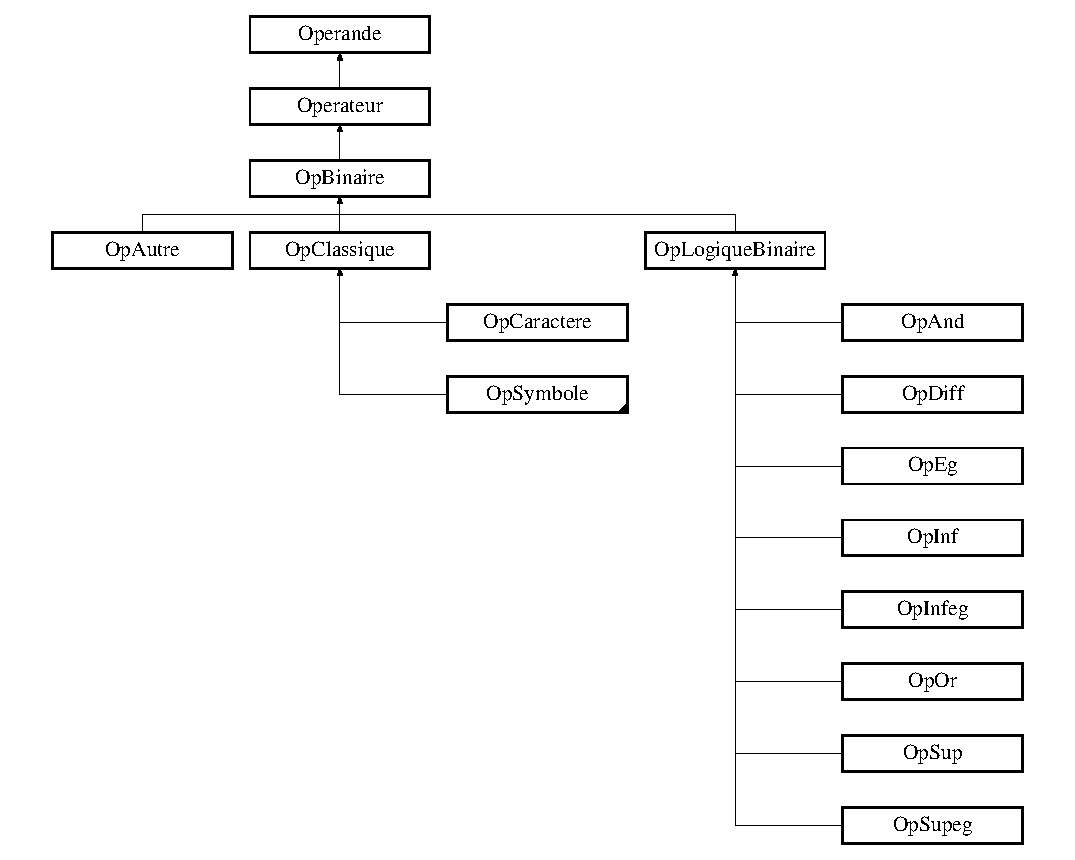
\includegraphics[height=11.107438cm]{class_op_binaire}
\end{center}
\end{figure}
\subsection*{Public Member Functions}
\begin{DoxyCompactItemize}
\item 
\hyperlink{class_op_binaire_ac70aab4bf3d8f220bcb164027b4bb404}{Op\+Binaire} (const Q\+String \&na)
\item 
virtual \hyperlink{class_op_binaire_af92a746a738f8f56ca1e402d3c2b529b}{$\sim$\+Op\+Binaire} ()
\item 
\hyperlink{class_litterale}{Litterale} $\ast$ \hyperlink{class_op_binaire_aa81570ae3aeb44b9533e7ddd82a397be}{executer} ()
\item 
virtual \hyperlink{class_litterale}{Litterale} $\ast$ \hyperlink{class_op_binaire_afb16dbd5f455b97afb5c07fae29b94fc}{fonction\+Num} (\hyperlink{class_nombres}{Nombres} $\ast$arg1, \hyperlink{class_litterale}{Litterale} $\ast$arg2)=0
\item 
virtual \hyperlink{class_litterale}{Litterale} $\ast$ \hyperlink{class_op_binaire_a72ea45bf3157516edeca687668d83b32}{fonction\+Expression} (\hyperlink{class_lit_expression}{Lit\+Expression} $\ast$arg1, \hyperlink{class_litterale}{Litterale} $\ast$arg2)=0
\item 
void \hyperlink{class_op_binaire_ac48be97498d47266542ff81c86c1a118}{add\+Arg} (\hyperlink{class_pile}{Pile} $\ast$pile)
\item 
void \hyperlink{class_op_binaire_af39b73a32c35ed7722fac1d380b92bbd}{add\+Arg} (\hyperlink{class_litterale}{Litterale} $\ast$arg)
\end{DoxyCompactItemize}
\subsection*{Additional Inherited Members}


\subsection{Detailed Description}


Definition at line 185 of file operator.\+h.



\subsection{Constructor \& Destructor Documentation}
\index{Op\+Binaire@{Op\+Binaire}!Op\+Binaire@{Op\+Binaire}}
\index{Op\+Binaire@{Op\+Binaire}!Op\+Binaire@{Op\+Binaire}}
\subsubsection[{\texorpdfstring{Op\+Binaire(const Q\+String \&na)}{OpBinaire(const QString &na)}}]{\setlength{\rightskip}{0pt plus 5cm}Op\+Binaire\+::\+Op\+Binaire (
\begin{DoxyParamCaption}
\item[{const Q\+String \&}]{na}
\end{DoxyParamCaption}
)\hspace{0.3cm}{\ttfamily [inline]}}\hypertarget{class_op_binaire_ac70aab4bf3d8f220bcb164027b4bb404}{}\label{class_op_binaire_ac70aab4bf3d8f220bcb164027b4bb404}


Definition at line 188 of file operator.\+h.

\index{Op\+Binaire@{Op\+Binaire}!````~Op\+Binaire@{$\sim$\+Op\+Binaire}}
\index{````~Op\+Binaire@{$\sim$\+Op\+Binaire}!Op\+Binaire@{Op\+Binaire}}
\subsubsection[{\texorpdfstring{$\sim$\+Op\+Binaire()}{~OpBinaire()}}]{\setlength{\rightskip}{0pt plus 5cm}Op\+Binaire\+::$\sim$\+Op\+Binaire (
\begin{DoxyParamCaption}
{}
\end{DoxyParamCaption}
)\hspace{0.3cm}{\ttfamily [virtual]}}\hypertarget{class_op_binaire_af92a746a738f8f56ca1e402d3c2b529b}{}\label{class_op_binaire_af92a746a738f8f56ca1e402d3c2b529b}


Definition at line 210 of file operator.\+cpp.



\subsection{Member Function Documentation}
\index{Op\+Binaire@{Op\+Binaire}!add\+Arg@{add\+Arg}}
\index{add\+Arg@{add\+Arg}!Op\+Binaire@{Op\+Binaire}}
\subsubsection[{\texorpdfstring{add\+Arg(\+Pile $\ast$pile)}{addArg(Pile *pile)}}]{\setlength{\rightskip}{0pt plus 5cm}void Op\+Binaire\+::add\+Arg (
\begin{DoxyParamCaption}
\item[{{\bf Pile} $\ast$}]{pile}
\end{DoxyParamCaption}
)\hspace{0.3cm}{\ttfamily [virtual]}}\hypertarget{class_op_binaire_ac48be97498d47266542ff81c86c1a118}{}\label{class_op_binaire_ac48be97498d47266542ff81c86c1a118}


Reimplemented from \hyperlink{class_operateur_ae9b209c3a9f55eb3b3821f43fe437105}{Operateur}.



Definition at line 214 of file operator.\+cpp.

\index{Op\+Binaire@{Op\+Binaire}!add\+Arg@{add\+Arg}}
\index{add\+Arg@{add\+Arg}!Op\+Binaire@{Op\+Binaire}}
\subsubsection[{\texorpdfstring{add\+Arg(\+Litterale $\ast$arg)}{addArg(Litterale *arg)}}]{\setlength{\rightskip}{0pt plus 5cm}void Op\+Binaire\+::add\+Arg (
\begin{DoxyParamCaption}
\item[{{\bf Litterale} $\ast$}]{arg}
\end{DoxyParamCaption}
)\hspace{0.3cm}{\ttfamily [virtual]}}\hypertarget{class_op_binaire_af39b73a32c35ed7722fac1d380b92bbd}{}\label{class_op_binaire_af39b73a32c35ed7722fac1d380b92bbd}


Reimplemented from \hyperlink{class_operateur_ae39d95062e174881d250561617cf7a6a}{Operateur}.



Definition at line 221 of file operator.\+cpp.

\index{Op\+Binaire@{Op\+Binaire}!executer@{executer}}
\index{executer@{executer}!Op\+Binaire@{Op\+Binaire}}
\subsubsection[{\texorpdfstring{executer()}{executer()}}]{\setlength{\rightskip}{0pt plus 5cm}{\bf Litterale} $\ast$ Op\+Binaire\+::executer (
\begin{DoxyParamCaption}
{}
\end{DoxyParamCaption}
)\hspace{0.3cm}{\ttfamily [virtual]}}\hypertarget{class_op_binaire_aa81570ae3aeb44b9533e7ddd82a397be}{}\label{class_op_binaire_aa81570ae3aeb44b9533e7ddd82a397be}


Implements \hyperlink{class_operateur_a875ee3c8ad2284fd8537c32070d059d2}{Operateur}.



Definition at line 228 of file operator.\+cpp.

\index{Op\+Binaire@{Op\+Binaire}!fonction\+Expression@{fonction\+Expression}}
\index{fonction\+Expression@{fonction\+Expression}!Op\+Binaire@{Op\+Binaire}}
\subsubsection[{\texorpdfstring{fonction\+Expression(\+Lit\+Expression $\ast$arg1, Litterale $\ast$arg2)=0}{fonctionExpression(LitExpression *arg1, Litterale *arg2)=0}}]{\setlength{\rightskip}{0pt plus 5cm}virtual {\bf Litterale}$\ast$ Op\+Binaire\+::fonction\+Expression (
\begin{DoxyParamCaption}
\item[{{\bf Lit\+Expression} $\ast$}]{arg1, }
\item[{{\bf Litterale} $\ast$}]{arg2}
\end{DoxyParamCaption}
)\hspace{0.3cm}{\ttfamily [pure virtual]}}\hypertarget{class_op_binaire_a72ea45bf3157516edeca687668d83b32}{}\label{class_op_binaire_a72ea45bf3157516edeca687668d83b32}


Implemented in \hyperlink{class_op_caractere_ae79a9c802c54f07d7650603c58d44eff}{Op\+Caractere}, \hyperlink{class_op_symbole_a0b9eb81e1a88d0d1470f642c7afa2b8c}{Op\+Symbole}, \hyperlink{class_op_classique_aad9c17d4a2744d7e1afe6802fbbc3cdd}{Op\+Classique}, and \hyperlink{class_op_logique_binaire_a4fbde2ff67fe7f2bfa1898522158bff1}{Op\+Logique\+Binaire}.

\index{Op\+Binaire@{Op\+Binaire}!fonction\+Num@{fonction\+Num}}
\index{fonction\+Num@{fonction\+Num}!Op\+Binaire@{Op\+Binaire}}
\subsubsection[{\texorpdfstring{fonction\+Num(\+Nombres $\ast$arg1, Litterale $\ast$arg2)=0}{fonctionNum(Nombres *arg1, Litterale *arg2)=0}}]{\setlength{\rightskip}{0pt plus 5cm}virtual {\bf Litterale}$\ast$ Op\+Binaire\+::fonction\+Num (
\begin{DoxyParamCaption}
\item[{{\bf Nombres} $\ast$}]{arg1, }
\item[{{\bf Litterale} $\ast$}]{arg2}
\end{DoxyParamCaption}
)\hspace{0.3cm}{\ttfamily [pure virtual]}}\hypertarget{class_op_binaire_afb16dbd5f455b97afb5c07fae29b94fc}{}\label{class_op_binaire_afb16dbd5f455b97afb5c07fae29b94fc}


Implemented in \hyperlink{class_op_div_a2607c7a6356f4a3d358070b924e077ad}{Op\+Div}, \hyperlink{class_op_caractere_a1bf53676903dbdcff31c9528f5cf09c7}{Op\+Caractere}, \hyperlink{class_op_symbole_ae908fd3da24f9cc8aa93f87360e07009}{Op\+Symbole}, \hyperlink{class_op_classique_a79bb2899f581c5773056611216a6ef7b}{Op\+Classique}, and \hyperlink{class_op_logique_binaire_a5565bc1dd13c6bddea8b91995dda703a}{Op\+Logique\+Binaire}.



The documentation for this class was generated from the following files\+:\begin{DoxyCompactItemize}
\item 
\hyperlink{operator_8h}{operator.\+h}\item 
\hyperlink{operator_8cpp}{operator.\+cpp}\end{DoxyCompactItemize}

\hypertarget{class_op_caractere}{}\section{Op\+Caractere Class Reference}
\label{class_op_caractere}\index{Op\+Caractere@{Op\+Caractere}}


{\ttfamily \#include $<$operator\+Classique.\+h$>$}

Inheritance diagram for Op\+Caractere\+:\begin{figure}[H]
\begin{center}
\leavevmode
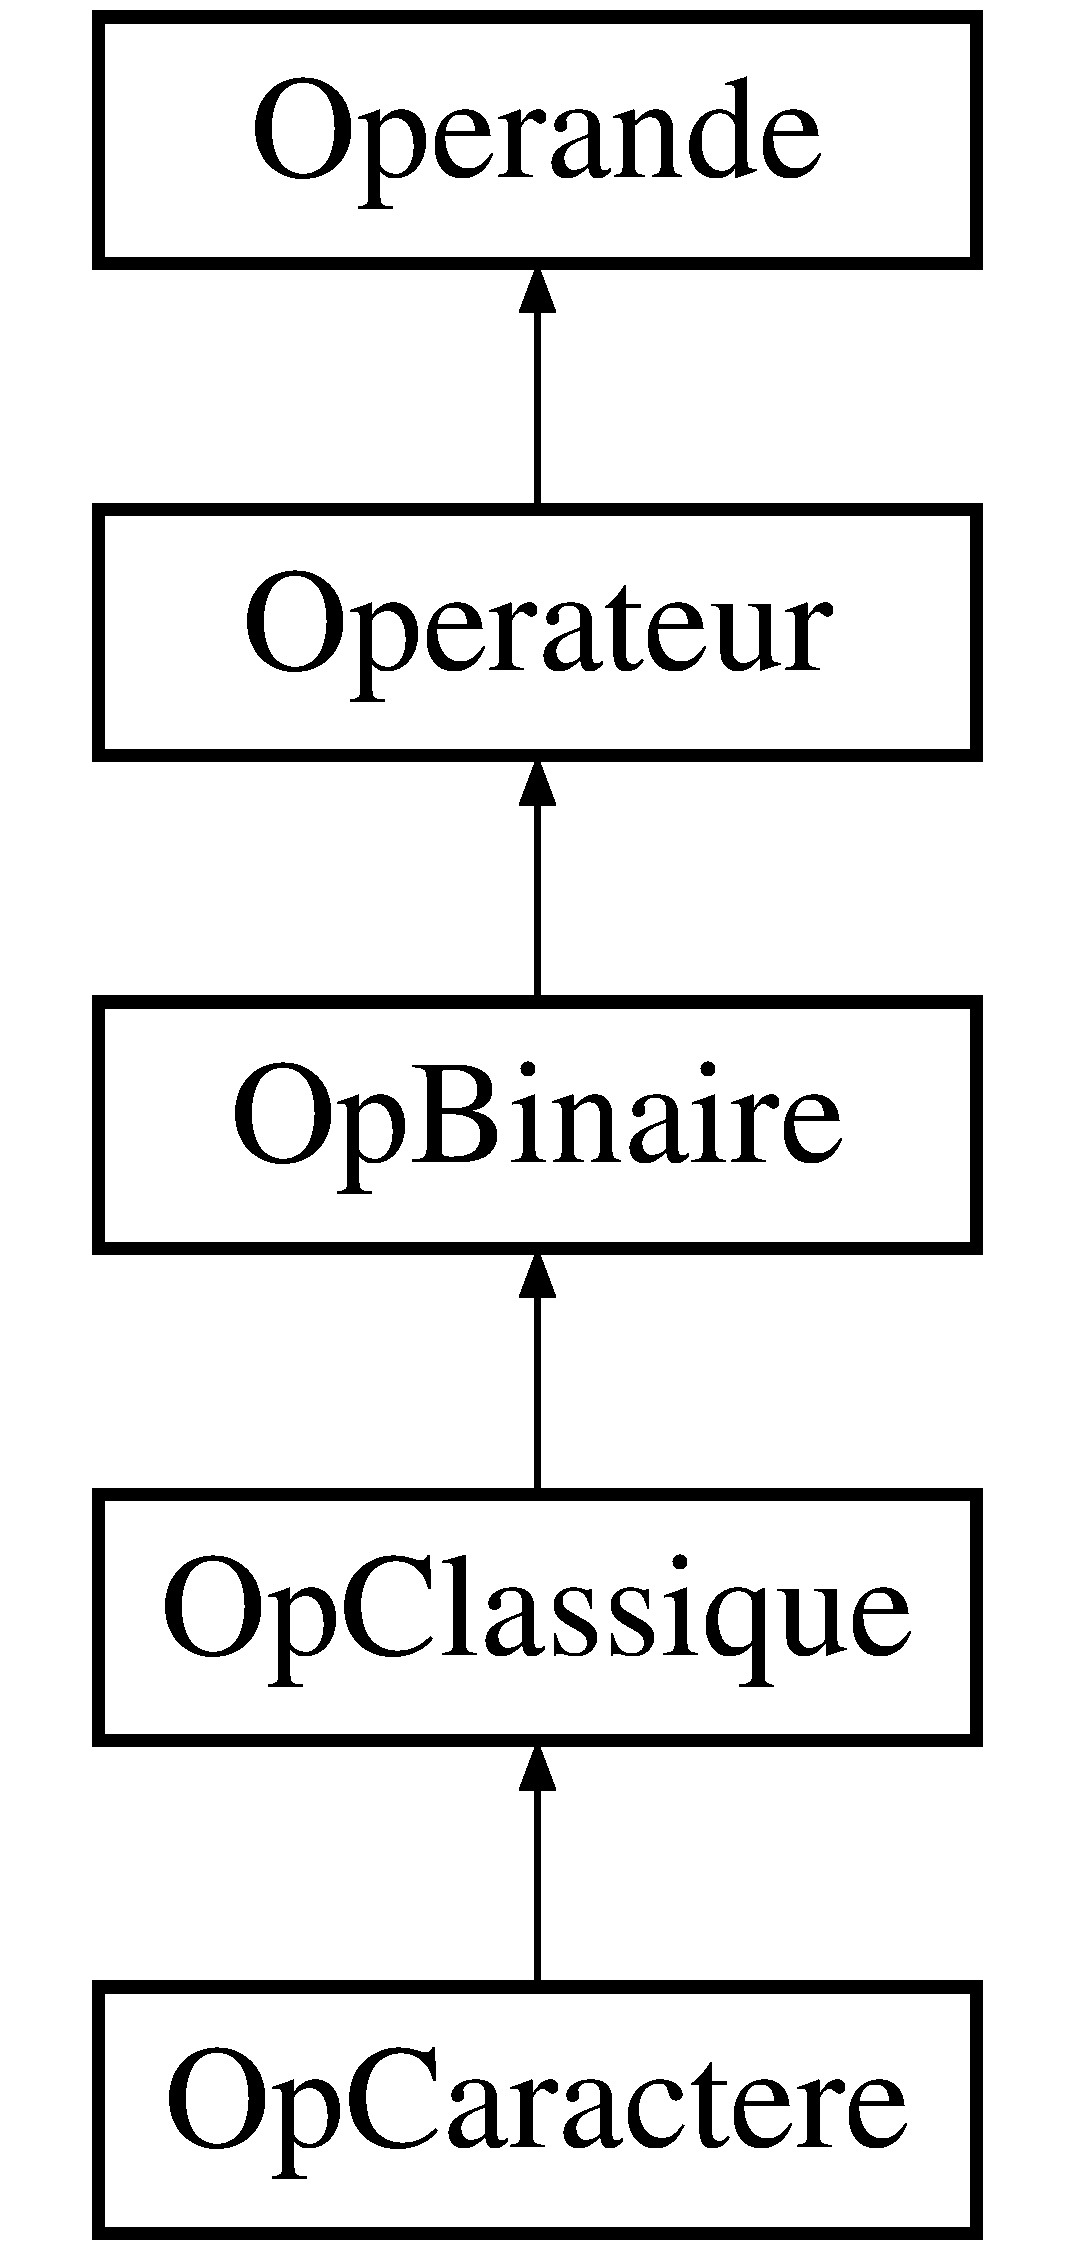
\includegraphics[height=5.000000cm]{class_op_caractere}
\end{center}
\end{figure}
\subsection*{Public Member Functions}
\begin{DoxyCompactItemize}
\item 
\hyperlink{class_op_caractere_a63c38dc6f6843f6a5d13d9c66551fb59}{Op\+Caractere} (const Q\+String \&na)
\item 
virtual \hyperlink{class_litterale}{Litterale} $\ast$ \hyperlink{class_op_caractere_a1bf53676903dbdcff31c9528f5cf09c7}{fonction\+Num} (\hyperlink{class_nombres}{Nombres} $\ast$arg1, \hyperlink{class_litterale}{Litterale} $\ast$arg2)
\item 
virtual \hyperlink{class_litterale}{Litterale} $\ast$ \hyperlink{class_op_caractere_a1bd2534371e5d09150131ab4ceb31013}{fonction\+Num2} (\hyperlink{class_entier}{Entier} $\ast$arg1, \hyperlink{class_litterale}{Litterale} $\ast$arg2)
\item 
virtual \hyperlink{class_litterale}{Litterale} $\ast$ \hyperlink{class_op_caractere_aea29b98d94bb1b4d26c38a77cddeec3c}{fonction\+Num2} (\hyperlink{class_reelle}{Reelle} $\ast$arg1, \hyperlink{class_litterale}{Litterale} $\ast$arg2)
\item 
virtual \hyperlink{class_litterale}{Litterale} $\ast$ \hyperlink{class_op_caractere_a9939635a4bd04ae96ef07a57991b665d}{fonction\+Num2} (\hyperlink{class_rationnelle}{Rationnelle} $\ast$arg1, \hyperlink{class_litterale}{Litterale} $\ast$arg2)
\item 
\hyperlink{class_litterale}{Litterale} $\ast$ \hyperlink{class_op_caractere_ae79a9c802c54f07d7650603c58d44eff}{fonction\+Expression} (\hyperlink{class_lit_expression}{Lit\+Expression} $\ast$arg1, \hyperlink{class_litterale}{Litterale} $\ast$arg2)
\item 
virtual \hyperlink{class_litterale}{Litterale} $\ast$ \hyperlink{class_op_caractere_ab223e679ae6fc710dd1c0297bafa893a}{action\+Num} (\hyperlink{class_entier}{Entier} \&arg1, \hyperlink{class_entier}{Entier} \&arg2)=0
\item 
virtual \hyperlink{class_litterale}{Litterale} $\ast$ \hyperlink{class_op_caractere_aa2cfbd2038de905702b9d83d7d926cdc}{action\+Num} (\hyperlink{class_entier}{Entier} \&arg1, \hyperlink{class_reelle}{Reelle} \&arg2)=0
\item 
virtual \hyperlink{class_litterale}{Litterale} $\ast$ \hyperlink{class_op_caractere_a4e5b229898e12c67082ba8bc3860710c}{action\+Num} (\hyperlink{class_entier}{Entier} \&arg1, \hyperlink{class_rationnelle}{Rationnelle} \&arg2)=0
\item 
virtual \hyperlink{class_litterale}{Litterale} $\ast$ \hyperlink{class_op_caractere_a934b6964376e4d4075520e92c95f8717}{action\+Num} (\hyperlink{class_reelle}{Reelle} \&arg1, \hyperlink{class_reelle}{Reelle} \&arg2)=0
\item 
virtual \hyperlink{class_litterale}{Litterale} $\ast$ \hyperlink{class_op_caractere_a2a0bd1973a044196ec0de3503fb46438}{action\+Num} (\hyperlink{class_reelle}{Reelle} \&arg1, \hyperlink{class_entier}{Entier} \&arg2)=0
\item 
virtual \hyperlink{class_litterale}{Litterale} $\ast$ \hyperlink{class_op_caractere_a7f7fd7ffda4599eefda1c1811e71fce9}{action\+Num} (\hyperlink{class_reelle}{Reelle} \&arg1, \hyperlink{class_rationnelle}{Rationnelle} \&arg2)=0
\item 
virtual \hyperlink{class_litterale}{Litterale} $\ast$ \hyperlink{class_op_caractere_a17df3c470b50a418111766eaf8159fd3}{action\+Num} (\hyperlink{class_rationnelle}{Rationnelle} \&arg1, \hyperlink{class_rationnelle}{Rationnelle} \&arg2)=0
\item 
virtual \hyperlink{class_litterale}{Litterale} $\ast$ \hyperlink{class_op_caractere_a40a4928d9d1c5024d9a90760333db3e8}{action\+Num} (\hyperlink{class_rationnelle}{Rationnelle} \&arg1, \hyperlink{class_entier}{Entier} \&arg2)=0
\item 
virtual \hyperlink{class_litterale}{Litterale} $\ast$ \hyperlink{class_op_caractere_a11959ee28e27d686eefe5f80307255b5}{action\+Num} (\hyperlink{class_rationnelle}{Rationnelle} \&arg1, \hyperlink{class_reelle}{Reelle} \&arg2)=0
\end{DoxyCompactItemize}
\subsection*{Additional Inherited Members}


\subsection{Detailed Description}


Definition at line 40 of file operator\+Classique.\+h.



\subsection{Constructor \& Destructor Documentation}
\index{Op\+Caractere@{Op\+Caractere}!Op\+Caractere@{Op\+Caractere}}
\index{Op\+Caractere@{Op\+Caractere}!Op\+Caractere@{Op\+Caractere}}
\subsubsection[{\texorpdfstring{Op\+Caractere(const Q\+String \&na)}{OpCaractere(const QString &na)}}]{\setlength{\rightskip}{0pt plus 5cm}Op\+Caractere\+::\+Op\+Caractere (
\begin{DoxyParamCaption}
\item[{const Q\+String \&}]{na}
\end{DoxyParamCaption}
)\hspace{0.3cm}{\ttfamily [inline]}}\hypertarget{class_op_caractere_a63c38dc6f6843f6a5d13d9c66551fb59}{}\label{class_op_caractere_a63c38dc6f6843f6a5d13d9c66551fb59}


Definition at line 42 of file operator\+Classique.\+h.



\subsection{Member Function Documentation}
\index{Op\+Caractere@{Op\+Caractere}!action\+Num@{action\+Num}}
\index{action\+Num@{action\+Num}!Op\+Caractere@{Op\+Caractere}}
\subsubsection[{\texorpdfstring{action\+Num(\+Entier \&arg1, Entier \&arg2)=0}{actionNum(Entier &arg1, Entier &arg2)=0}}]{\setlength{\rightskip}{0pt plus 5cm}virtual {\bf Litterale}$\ast$ Op\+Caractere\+::action\+Num (
\begin{DoxyParamCaption}
\item[{{\bf Entier} \&}]{arg1, }
\item[{{\bf Entier} \&}]{arg2}
\end{DoxyParamCaption}
)\hspace{0.3cm}{\ttfamily [pure virtual]}}\hypertarget{class_op_caractere_ab223e679ae6fc710dd1c0297bafa893a}{}\label{class_op_caractere_ab223e679ae6fc710dd1c0297bafa893a}
\index{Op\+Caractere@{Op\+Caractere}!action\+Num@{action\+Num}}
\index{action\+Num@{action\+Num}!Op\+Caractere@{Op\+Caractere}}
\subsubsection[{\texorpdfstring{action\+Num(\+Entier \&arg1, Reelle \&arg2)=0}{actionNum(Entier &arg1, Reelle &arg2)=0}}]{\setlength{\rightskip}{0pt plus 5cm}virtual {\bf Litterale}$\ast$ Op\+Caractere\+::action\+Num (
\begin{DoxyParamCaption}
\item[{{\bf Entier} \&}]{arg1, }
\item[{{\bf Reelle} \&}]{arg2}
\end{DoxyParamCaption}
)\hspace{0.3cm}{\ttfamily [pure virtual]}}\hypertarget{class_op_caractere_aa2cfbd2038de905702b9d83d7d926cdc}{}\label{class_op_caractere_aa2cfbd2038de905702b9d83d7d926cdc}
\index{Op\+Caractere@{Op\+Caractere}!action\+Num@{action\+Num}}
\index{action\+Num@{action\+Num}!Op\+Caractere@{Op\+Caractere}}
\subsubsection[{\texorpdfstring{action\+Num(\+Entier \&arg1, Rationnelle \&arg2)=0}{actionNum(Entier &arg1, Rationnelle &arg2)=0}}]{\setlength{\rightskip}{0pt plus 5cm}virtual {\bf Litterale}$\ast$ Op\+Caractere\+::action\+Num (
\begin{DoxyParamCaption}
\item[{{\bf Entier} \&}]{arg1, }
\item[{{\bf Rationnelle} \&}]{arg2}
\end{DoxyParamCaption}
)\hspace{0.3cm}{\ttfamily [pure virtual]}}\hypertarget{class_op_caractere_a4e5b229898e12c67082ba8bc3860710c}{}\label{class_op_caractere_a4e5b229898e12c67082ba8bc3860710c}
\index{Op\+Caractere@{Op\+Caractere}!action\+Num@{action\+Num}}
\index{action\+Num@{action\+Num}!Op\+Caractere@{Op\+Caractere}}
\subsubsection[{\texorpdfstring{action\+Num(\+Reelle \&arg1, Reelle \&arg2)=0}{actionNum(Reelle &arg1, Reelle &arg2)=0}}]{\setlength{\rightskip}{0pt plus 5cm}virtual {\bf Litterale}$\ast$ Op\+Caractere\+::action\+Num (
\begin{DoxyParamCaption}
\item[{{\bf Reelle} \&}]{arg1, }
\item[{{\bf Reelle} \&}]{arg2}
\end{DoxyParamCaption}
)\hspace{0.3cm}{\ttfamily [pure virtual]}}\hypertarget{class_op_caractere_a934b6964376e4d4075520e92c95f8717}{}\label{class_op_caractere_a934b6964376e4d4075520e92c95f8717}
\index{Op\+Caractere@{Op\+Caractere}!action\+Num@{action\+Num}}
\index{action\+Num@{action\+Num}!Op\+Caractere@{Op\+Caractere}}
\subsubsection[{\texorpdfstring{action\+Num(\+Reelle \&arg1, Entier \&arg2)=0}{actionNum(Reelle &arg1, Entier &arg2)=0}}]{\setlength{\rightskip}{0pt plus 5cm}virtual {\bf Litterale}$\ast$ Op\+Caractere\+::action\+Num (
\begin{DoxyParamCaption}
\item[{{\bf Reelle} \&}]{arg1, }
\item[{{\bf Entier} \&}]{arg2}
\end{DoxyParamCaption}
)\hspace{0.3cm}{\ttfamily [pure virtual]}}\hypertarget{class_op_caractere_a2a0bd1973a044196ec0de3503fb46438}{}\label{class_op_caractere_a2a0bd1973a044196ec0de3503fb46438}
\index{Op\+Caractere@{Op\+Caractere}!action\+Num@{action\+Num}}
\index{action\+Num@{action\+Num}!Op\+Caractere@{Op\+Caractere}}
\subsubsection[{\texorpdfstring{action\+Num(\+Reelle \&arg1, Rationnelle \&arg2)=0}{actionNum(Reelle &arg1, Rationnelle &arg2)=0}}]{\setlength{\rightskip}{0pt plus 5cm}virtual {\bf Litterale}$\ast$ Op\+Caractere\+::action\+Num (
\begin{DoxyParamCaption}
\item[{{\bf Reelle} \&}]{arg1, }
\item[{{\bf Rationnelle} \&}]{arg2}
\end{DoxyParamCaption}
)\hspace{0.3cm}{\ttfamily [pure virtual]}}\hypertarget{class_op_caractere_a7f7fd7ffda4599eefda1c1811e71fce9}{}\label{class_op_caractere_a7f7fd7ffda4599eefda1c1811e71fce9}
\index{Op\+Caractere@{Op\+Caractere}!action\+Num@{action\+Num}}
\index{action\+Num@{action\+Num}!Op\+Caractere@{Op\+Caractere}}
\subsubsection[{\texorpdfstring{action\+Num(\+Rationnelle \&arg1, Rationnelle \&arg2)=0}{actionNum(Rationnelle &arg1, Rationnelle &arg2)=0}}]{\setlength{\rightskip}{0pt plus 5cm}virtual {\bf Litterale}$\ast$ Op\+Caractere\+::action\+Num (
\begin{DoxyParamCaption}
\item[{{\bf Rationnelle} \&}]{arg1, }
\item[{{\bf Rationnelle} \&}]{arg2}
\end{DoxyParamCaption}
)\hspace{0.3cm}{\ttfamily [pure virtual]}}\hypertarget{class_op_caractere_a17df3c470b50a418111766eaf8159fd3}{}\label{class_op_caractere_a17df3c470b50a418111766eaf8159fd3}
\index{Op\+Caractere@{Op\+Caractere}!action\+Num@{action\+Num}}
\index{action\+Num@{action\+Num}!Op\+Caractere@{Op\+Caractere}}
\subsubsection[{\texorpdfstring{action\+Num(\+Rationnelle \&arg1, Entier \&arg2)=0}{actionNum(Rationnelle &arg1, Entier &arg2)=0}}]{\setlength{\rightskip}{0pt plus 5cm}virtual {\bf Litterale}$\ast$ Op\+Caractere\+::action\+Num (
\begin{DoxyParamCaption}
\item[{{\bf Rationnelle} \&}]{arg1, }
\item[{{\bf Entier} \&}]{arg2}
\end{DoxyParamCaption}
)\hspace{0.3cm}{\ttfamily [pure virtual]}}\hypertarget{class_op_caractere_a40a4928d9d1c5024d9a90760333db3e8}{}\label{class_op_caractere_a40a4928d9d1c5024d9a90760333db3e8}
\index{Op\+Caractere@{Op\+Caractere}!action\+Num@{action\+Num}}
\index{action\+Num@{action\+Num}!Op\+Caractere@{Op\+Caractere}}
\subsubsection[{\texorpdfstring{action\+Num(\+Rationnelle \&arg1, Reelle \&arg2)=0}{actionNum(Rationnelle &arg1, Reelle &arg2)=0}}]{\setlength{\rightskip}{0pt plus 5cm}virtual {\bf Litterale}$\ast$ Op\+Caractere\+::action\+Num (
\begin{DoxyParamCaption}
\item[{{\bf Rationnelle} \&}]{arg1, }
\item[{{\bf Reelle} \&}]{arg2}
\end{DoxyParamCaption}
)\hspace{0.3cm}{\ttfamily [pure virtual]}}\hypertarget{class_op_caractere_a11959ee28e27d686eefe5f80307255b5}{}\label{class_op_caractere_a11959ee28e27d686eefe5f80307255b5}
\index{Op\+Caractere@{Op\+Caractere}!fonction\+Expression@{fonction\+Expression}}
\index{fonction\+Expression@{fonction\+Expression}!Op\+Caractere@{Op\+Caractere}}
\subsubsection[{\texorpdfstring{fonction\+Expression(\+Lit\+Expression $\ast$arg1, Litterale $\ast$arg2)}{fonctionExpression(LitExpression *arg1, Litterale *arg2)}}]{\setlength{\rightskip}{0pt plus 5cm}{\bf Litterale} $\ast$ Op\+Caractere\+::fonction\+Expression (
\begin{DoxyParamCaption}
\item[{{\bf Lit\+Expression} $\ast$}]{arg1, }
\item[{{\bf Litterale} $\ast$}]{arg2}
\end{DoxyParamCaption}
)\hspace{0.3cm}{\ttfamily [virtual]}}\hypertarget{class_op_caractere_ae79a9c802c54f07d7650603c58d44eff}{}\label{class_op_caractere_ae79a9c802c54f07d7650603c58d44eff}


Implements \hyperlink{class_op_classique_aad9c17d4a2744d7e1afe6802fbbc3cdd}{Op\+Classique}.



Definition at line 65 of file operator\+Classique.\+cpp.

\index{Op\+Caractere@{Op\+Caractere}!fonction\+Num@{fonction\+Num}}
\index{fonction\+Num@{fonction\+Num}!Op\+Caractere@{Op\+Caractere}}
\subsubsection[{\texorpdfstring{fonction\+Num(\+Nombres $\ast$arg1, Litterale $\ast$arg2)}{fonctionNum(Nombres *arg1, Litterale *arg2)}}]{\setlength{\rightskip}{0pt plus 5cm}{\bf Litterale} $\ast$ Op\+Caractere\+::fonction\+Num (
\begin{DoxyParamCaption}
\item[{{\bf Nombres} $\ast$}]{arg1, }
\item[{{\bf Litterale} $\ast$}]{arg2}
\end{DoxyParamCaption}
)\hspace{0.3cm}{\ttfamily [virtual]}}\hypertarget{class_op_caractere_a1bf53676903dbdcff31c9528f5cf09c7}{}\label{class_op_caractere_a1bf53676903dbdcff31c9528f5cf09c7}


Implements \hyperlink{class_op_classique_a79bb2899f581c5773056611216a6ef7b}{Op\+Classique}.



Definition at line 44 of file operator\+Classique.\+cpp.

\index{Op\+Caractere@{Op\+Caractere}!fonction\+Num2@{fonction\+Num2}}
\index{fonction\+Num2@{fonction\+Num2}!Op\+Caractere@{Op\+Caractere}}
\subsubsection[{\texorpdfstring{fonction\+Num2(\+Entier $\ast$arg1, Litterale $\ast$arg2)}{fonctionNum2(Entier *arg1, Litterale *arg2)}}]{\setlength{\rightskip}{0pt plus 5cm}{\bf Litterale} $\ast$ Op\+Caractere\+::fonction\+Num2 (
\begin{DoxyParamCaption}
\item[{{\bf Entier} $\ast$}]{arg1, }
\item[{{\bf Litterale} $\ast$}]{arg2}
\end{DoxyParamCaption}
)\hspace{0.3cm}{\ttfamily [virtual]}}\hypertarget{class_op_caractere_a1bd2534371e5d09150131ab4ceb31013}{}\label{class_op_caractere_a1bd2534371e5d09150131ab4ceb31013}


Definition at line 49 of file operator\+Classique.\+cpp.

\index{Op\+Caractere@{Op\+Caractere}!fonction\+Num2@{fonction\+Num2}}
\index{fonction\+Num2@{fonction\+Num2}!Op\+Caractere@{Op\+Caractere}}
\subsubsection[{\texorpdfstring{fonction\+Num2(\+Reelle $\ast$arg1, Litterale $\ast$arg2)}{fonctionNum2(Reelle *arg1, Litterale *arg2)}}]{\setlength{\rightskip}{0pt plus 5cm}{\bf Litterale} $\ast$ Op\+Caractere\+::fonction\+Num2 (
\begin{DoxyParamCaption}
\item[{{\bf Reelle} $\ast$}]{arg1, }
\item[{{\bf Litterale} $\ast$}]{arg2}
\end{DoxyParamCaption}
)\hspace{0.3cm}{\ttfamily [virtual]}}\hypertarget{class_op_caractere_aea29b98d94bb1b4d26c38a77cddeec3c}{}\label{class_op_caractere_aea29b98d94bb1b4d26c38a77cddeec3c}


Definition at line 54 of file operator\+Classique.\+cpp.

\index{Op\+Caractere@{Op\+Caractere}!fonction\+Num2@{fonction\+Num2}}
\index{fonction\+Num2@{fonction\+Num2}!Op\+Caractere@{Op\+Caractere}}
\subsubsection[{\texorpdfstring{fonction\+Num2(\+Rationnelle $\ast$arg1, Litterale $\ast$arg2)}{fonctionNum2(Rationnelle *arg1, Litterale *arg2)}}]{\setlength{\rightskip}{0pt plus 5cm}{\bf Litterale} $\ast$ Op\+Caractere\+::fonction\+Num2 (
\begin{DoxyParamCaption}
\item[{{\bf Rationnelle} $\ast$}]{arg1, }
\item[{{\bf Litterale} $\ast$}]{arg2}
\end{DoxyParamCaption}
)\hspace{0.3cm}{\ttfamily [virtual]}}\hypertarget{class_op_caractere_a9939635a4bd04ae96ef07a57991b665d}{}\label{class_op_caractere_a9939635a4bd04ae96ef07a57991b665d}


Definition at line 59 of file operator\+Classique.\+cpp.



The documentation for this class was generated from the following files\+:\begin{DoxyCompactItemize}
\item 
\hyperlink{operator_classique_8h}{operator\+Classique.\+h}\item 
\hyperlink{operator_classique_8cpp}{operator\+Classique.\+cpp}\end{DoxyCompactItemize}

\hypertarget{class_op_classique}{}\section{Op\+Classique Class Reference}
\label{class_op_classique}\index{Op\+Classique@{Op\+Classique}}


{\ttfamily \#include $<$operator\+Classique.\+h$>$}

Inheritance diagram for Op\+Classique\+:\begin{figure}[H]
\begin{center}
\leavevmode
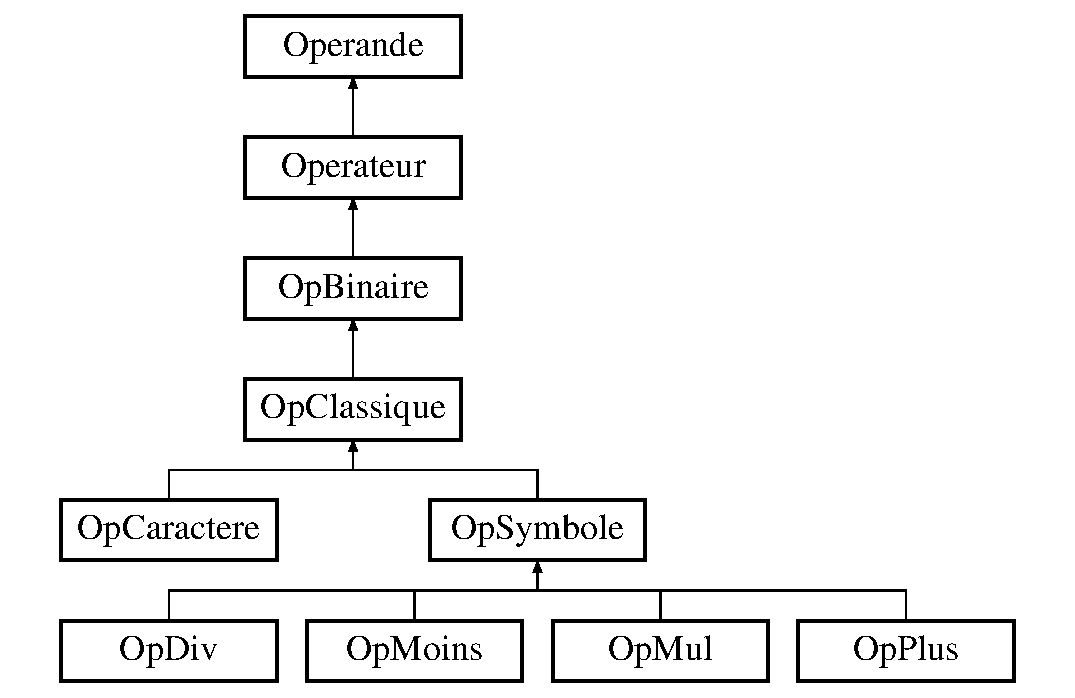
\includegraphics[height=6.000000cm]{class_op_classique}
\end{center}
\end{figure}
\subsection*{Public Member Functions}
\begin{DoxyCompactItemize}
\item 
\hyperlink{class_op_classique_a51e26a941922dfd08a8331a0c6d26adc}{Op\+Classique} (const Q\+String \&na)
\item 
virtual \hyperlink{class_litterale}{Litterale} $\ast$ \hyperlink{class_op_classique_a79bb2899f581c5773056611216a6ef7b}{fonction\+Num} (\hyperlink{class_nombres}{Nombres} $\ast$arg1, \hyperlink{class_litterale}{Litterale} $\ast$arg2)=0
\item 
virtual \hyperlink{class_litterale}{Litterale} $\ast$ \hyperlink{class_op_classique_aad9c17d4a2744d7e1afe6802fbbc3cdd}{fonction\+Expression} (\hyperlink{class_lit_expression}{Lit\+Expression} $\ast$arg1, \hyperlink{class_litterale}{Litterale} $\ast$arg2)=0
\end{DoxyCompactItemize}
\subsection*{Additional Inherited Members}


\subsection{Detailed Description}


Definition at line 11 of file operator\+Classique.\+h.



\subsection{Constructor \& Destructor Documentation}
\index{Op\+Classique@{Op\+Classique}!Op\+Classique@{Op\+Classique}}
\index{Op\+Classique@{Op\+Classique}!Op\+Classique@{Op\+Classique}}
\subsubsection[{\texorpdfstring{Op\+Classique(const Q\+String \&na)}{OpClassique(const QString &na)}}]{\setlength{\rightskip}{0pt plus 5cm}Op\+Classique\+::\+Op\+Classique (
\begin{DoxyParamCaption}
\item[{const Q\+String \&}]{na}
\end{DoxyParamCaption}
)\hspace{0.3cm}{\ttfamily [inline]}}\hypertarget{class_op_classique_a51e26a941922dfd08a8331a0c6d26adc}{}\label{class_op_classique_a51e26a941922dfd08a8331a0c6d26adc}


Definition at line 13 of file operator\+Classique.\+h.



\subsection{Member Function Documentation}
\index{Op\+Classique@{Op\+Classique}!fonction\+Expression@{fonction\+Expression}}
\index{fonction\+Expression@{fonction\+Expression}!Op\+Classique@{Op\+Classique}}
\subsubsection[{\texorpdfstring{fonction\+Expression(\+Lit\+Expression $\ast$arg1, Litterale $\ast$arg2)=0}{fonctionExpression(LitExpression *arg1, Litterale *arg2)=0}}]{\setlength{\rightskip}{0pt plus 5cm}virtual {\bf Litterale}$\ast$ Op\+Classique\+::fonction\+Expression (
\begin{DoxyParamCaption}
\item[{{\bf Lit\+Expression} $\ast$}]{arg1, }
\item[{{\bf Litterale} $\ast$}]{arg2}
\end{DoxyParamCaption}
)\hspace{0.3cm}{\ttfamily [pure virtual]}}\hypertarget{class_op_classique_aad9c17d4a2744d7e1afe6802fbbc3cdd}{}\label{class_op_classique_aad9c17d4a2744d7e1afe6802fbbc3cdd}


Implements \hyperlink{class_op_binaire_a72ea45bf3157516edeca687668d83b32}{Op\+Binaire}.



Implemented in \hyperlink{class_op_caractere_ae79a9c802c54f07d7650603c58d44eff}{Op\+Caractere}, and \hyperlink{class_op_symbole_a0b9eb81e1a88d0d1470f642c7afa2b8c}{Op\+Symbole}.

\index{Op\+Classique@{Op\+Classique}!fonction\+Num@{fonction\+Num}}
\index{fonction\+Num@{fonction\+Num}!Op\+Classique@{Op\+Classique}}
\subsubsection[{\texorpdfstring{fonction\+Num(\+Nombres $\ast$arg1, Litterale $\ast$arg2)=0}{fonctionNum(Nombres *arg1, Litterale *arg2)=0}}]{\setlength{\rightskip}{0pt plus 5cm}virtual {\bf Litterale}$\ast$ Op\+Classique\+::fonction\+Num (
\begin{DoxyParamCaption}
\item[{{\bf Nombres} $\ast$}]{arg1, }
\item[{{\bf Litterale} $\ast$}]{arg2}
\end{DoxyParamCaption}
)\hspace{0.3cm}{\ttfamily [pure virtual]}}\hypertarget{class_op_classique_a79bb2899f581c5773056611216a6ef7b}{}\label{class_op_classique_a79bb2899f581c5773056611216a6ef7b}


Implements \hyperlink{class_op_binaire_afb16dbd5f455b97afb5c07fae29b94fc}{Op\+Binaire}.



Implemented in \hyperlink{class_op_div_a2607c7a6356f4a3d358070b924e077ad}{Op\+Div}, \hyperlink{class_op_caractere_a1bf53676903dbdcff31c9528f5cf09c7}{Op\+Caractere}, and \hyperlink{class_op_symbole_ae908fd3da24f9cc8aa93f87360e07009}{Op\+Symbole}.



The documentation for this class was generated from the following file\+:\begin{DoxyCompactItemize}
\item 
\hyperlink{operator_classique_8h}{operator\+Classique.\+h}\end{DoxyCompactItemize}

\hypertarget{class_op_clear}{}\section{Op\+Clear Class Reference}
\label{class_op_clear}\index{Op\+Clear@{Op\+Clear}}


{\ttfamily \#include $<$operator.\+h$>$}

Inheritance diagram for Op\+Clear\+:\begin{figure}[H]
\begin{center}
\leavevmode
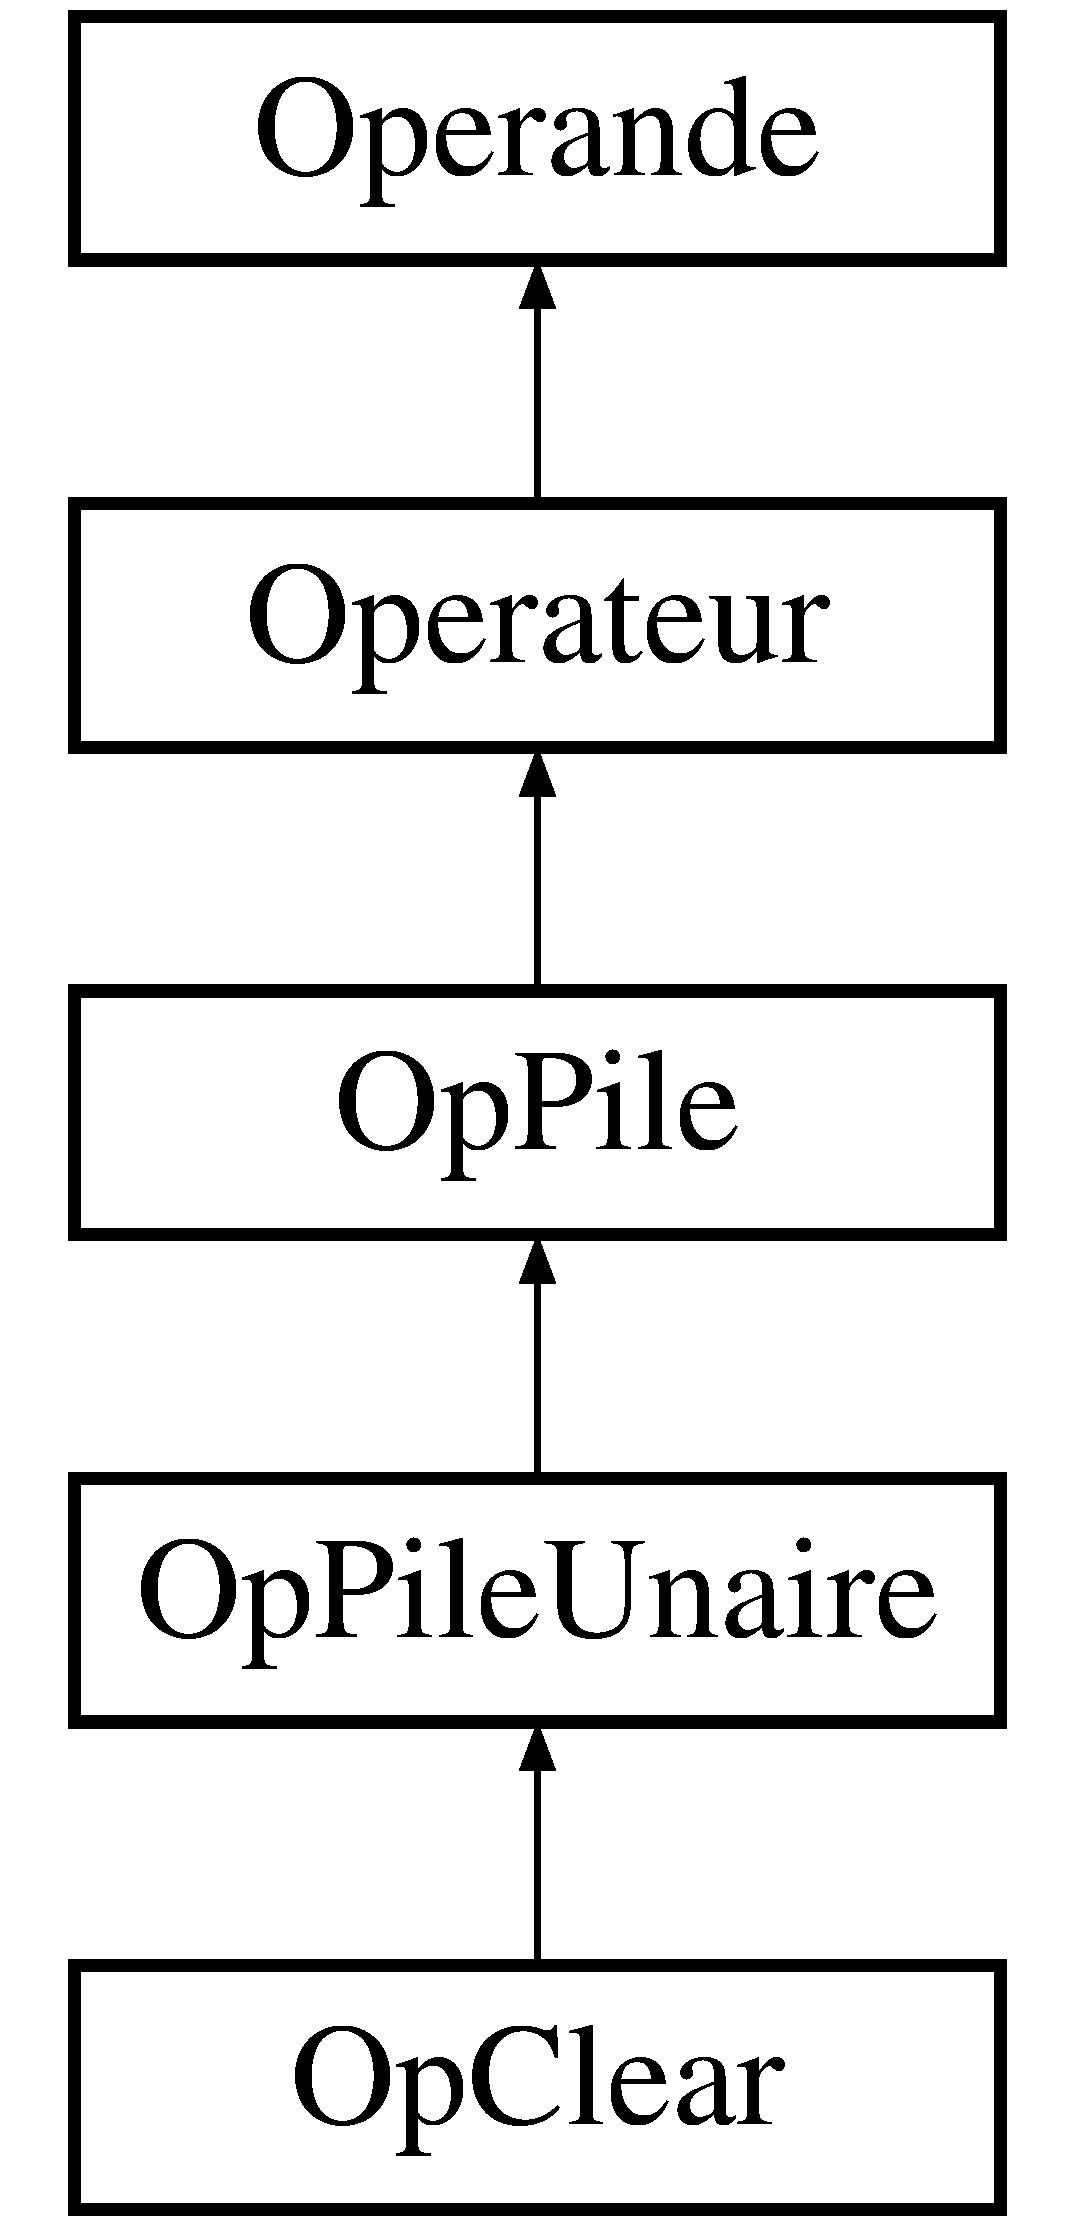
\includegraphics[height=5.000000cm]{class_op_clear}
\end{center}
\end{figure}
\subsection*{Public Member Functions}
\begin{DoxyCompactItemize}
\item 
\hyperlink{class_op_clear_a9dfd8594812e4e63d28e17be4e8d4199}{Op\+Clear} ()
\item 
void \hyperlink{class_op_clear_a4a8966c7fecc598a65a48947a61fa645}{executer\+Pile} ()
\end{DoxyCompactItemize}
\subsection*{Additional Inherited Members}


\subsection{Detailed Description}


Definition at line 239 of file operator.\+h.



\subsection{Constructor \& Destructor Documentation}
\index{Op\+Clear@{Op\+Clear}!Op\+Clear@{Op\+Clear}}
\index{Op\+Clear@{Op\+Clear}!Op\+Clear@{Op\+Clear}}
\subsubsection[{\texorpdfstring{Op\+Clear()}{OpClear()}}]{\setlength{\rightskip}{0pt plus 5cm}Op\+Clear\+::\+Op\+Clear (
\begin{DoxyParamCaption}
{}
\end{DoxyParamCaption}
)\hspace{0.3cm}{\ttfamily [inline]}}\hypertarget{class_op_clear_a9dfd8594812e4e63d28e17be4e8d4199}{}\label{class_op_clear_a9dfd8594812e4e63d28e17be4e8d4199}


Definition at line 241 of file operator.\+h.



\subsection{Member Function Documentation}
\index{Op\+Clear@{Op\+Clear}!executer\+Pile@{executer\+Pile}}
\index{executer\+Pile@{executer\+Pile}!Op\+Clear@{Op\+Clear}}
\subsubsection[{\texorpdfstring{executer\+Pile()}{executerPile()}}]{\setlength{\rightskip}{0pt plus 5cm}void Op\+Clear\+::executer\+Pile (
\begin{DoxyParamCaption}
{}
\end{DoxyParamCaption}
)\hspace{0.3cm}{\ttfamily [virtual]}}\hypertarget{class_op_clear_a4a8966c7fecc598a65a48947a61fa645}{}\label{class_op_clear_a4a8966c7fecc598a65a48947a61fa645}


Reimplemented from \hyperlink{class_op_pile_unaire_ae7f0b928350431fd080150a89312f3cf}{Op\+Pile\+Unaire}.



Definition at line 281 of file operator.\+cpp.



The documentation for this class was generated from the following files\+:\begin{DoxyCompactItemize}
\item 
\hyperlink{operator_8h}{operator.\+h}\item 
\hyperlink{operator_8cpp}{operator.\+cpp}\end{DoxyCompactItemize}

\hypertarget{class_op_clear_factory}{}\section{Op\+Clear\+Factory Class Reference}
\label{class_op_clear_factory}\index{Op\+Clear\+Factory@{Op\+Clear\+Factory}}


{\ttfamily \#include $<$operator\+Factory.\+h$>$}

Inheritance diagram for Op\+Clear\+Factory\+:\begin{figure}[H]
\begin{center}
\leavevmode
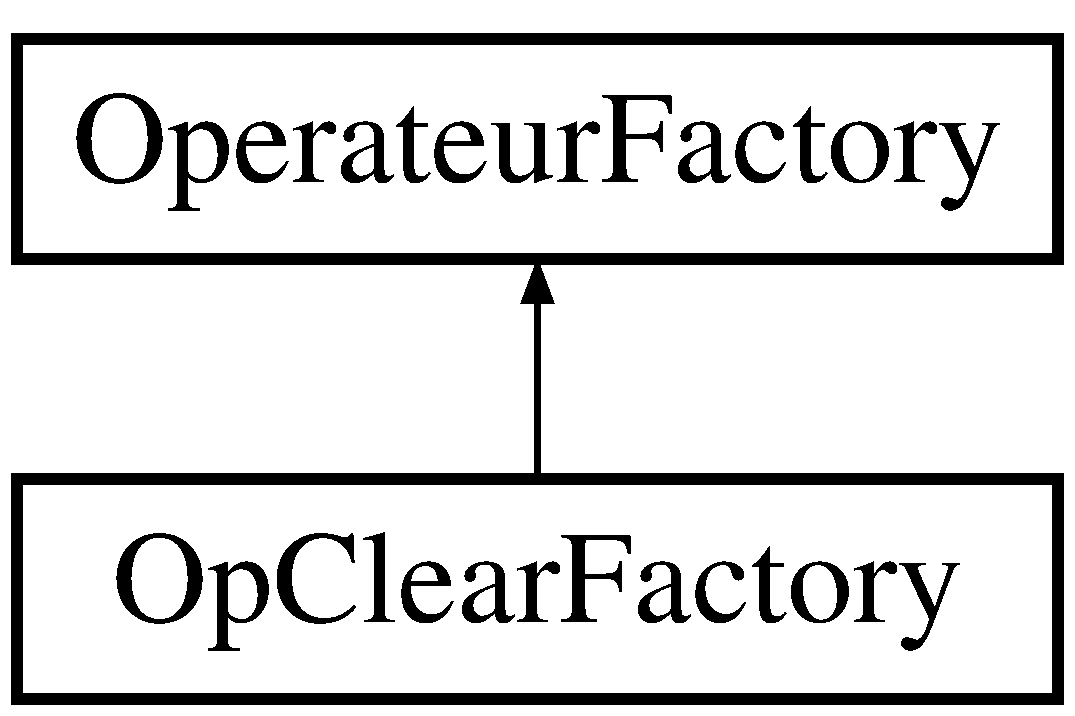
\includegraphics[height=2.000000cm]{class_op_clear_factory}
\end{center}
\end{figure}
\subsection*{Public Member Functions}
\begin{DoxyCompactItemize}
\item 
\hyperlink{class_op_clear_factory_a5fd88c9bda54361555d7a7b9420534b8}{Op\+Clear\+Factory} ()
\item 
\hyperlink{class_operateur}{Operateur} $\ast$ \hyperlink{class_op_clear_factory_abd8485d0461c7ae160bebbb3c7f18622}{get\+Operateur} ()
\end{DoxyCompactItemize}
\subsection*{Additional Inherited Members}


\subsection{Detailed Description}


Definition at line 135 of file operator\+Factory.\+h.



\subsection{Constructor \& Destructor Documentation}
\index{Op\+Clear\+Factory@{Op\+Clear\+Factory}!Op\+Clear\+Factory@{Op\+Clear\+Factory}}
\index{Op\+Clear\+Factory@{Op\+Clear\+Factory}!Op\+Clear\+Factory@{Op\+Clear\+Factory}}
\subsubsection[{\texorpdfstring{Op\+Clear\+Factory()}{OpClearFactory()}}]{\setlength{\rightskip}{0pt plus 5cm}Op\+Clear\+Factory\+::\+Op\+Clear\+Factory (
\begin{DoxyParamCaption}
{}
\end{DoxyParamCaption}
)\hspace{0.3cm}{\ttfamily [inline]}}\hypertarget{class_op_clear_factory_a5fd88c9bda54361555d7a7b9420534b8}{}\label{class_op_clear_factory_a5fd88c9bda54361555d7a7b9420534b8}


Definition at line 137 of file operator\+Factory.\+h.



\subsection{Member Function Documentation}
\index{Op\+Clear\+Factory@{Op\+Clear\+Factory}!get\+Operateur@{get\+Operateur}}
\index{get\+Operateur@{get\+Operateur}!Op\+Clear\+Factory@{Op\+Clear\+Factory}}
\subsubsection[{\texorpdfstring{get\+Operateur()}{getOperateur()}}]{\setlength{\rightskip}{0pt plus 5cm}{\bf Operateur}$\ast$ Op\+Clear\+Factory\+::get\+Operateur (
\begin{DoxyParamCaption}
{}
\end{DoxyParamCaption}
)\hspace{0.3cm}{\ttfamily [inline]}, {\ttfamily [virtual]}}\hypertarget{class_op_clear_factory_abd8485d0461c7ae160bebbb3c7f18622}{}\label{class_op_clear_factory_abd8485d0461c7ae160bebbb3c7f18622}


Implements \hyperlink{class_operateur_factory_aff61b2f67451f086d6abaea4231b2d78}{Operateur\+Factory}.



Definition at line 138 of file operator\+Factory.\+h.



The documentation for this class was generated from the following file\+:\begin{DoxyCompactItemize}
\item 
\hyperlink{operator_factory_8h}{operator\+Factory.\+h}\end{DoxyCompactItemize}

\hypertarget{class_op_diff}{}\section{Op\+Diff Class Reference}
\label{class_op_diff}\index{Op\+Diff@{Op\+Diff}}


{\ttfamily \#include $<$operator\+Logique.\+h$>$}

Inheritance diagram for Op\+Diff\+:\begin{figure}[H]
\begin{center}
\leavevmode
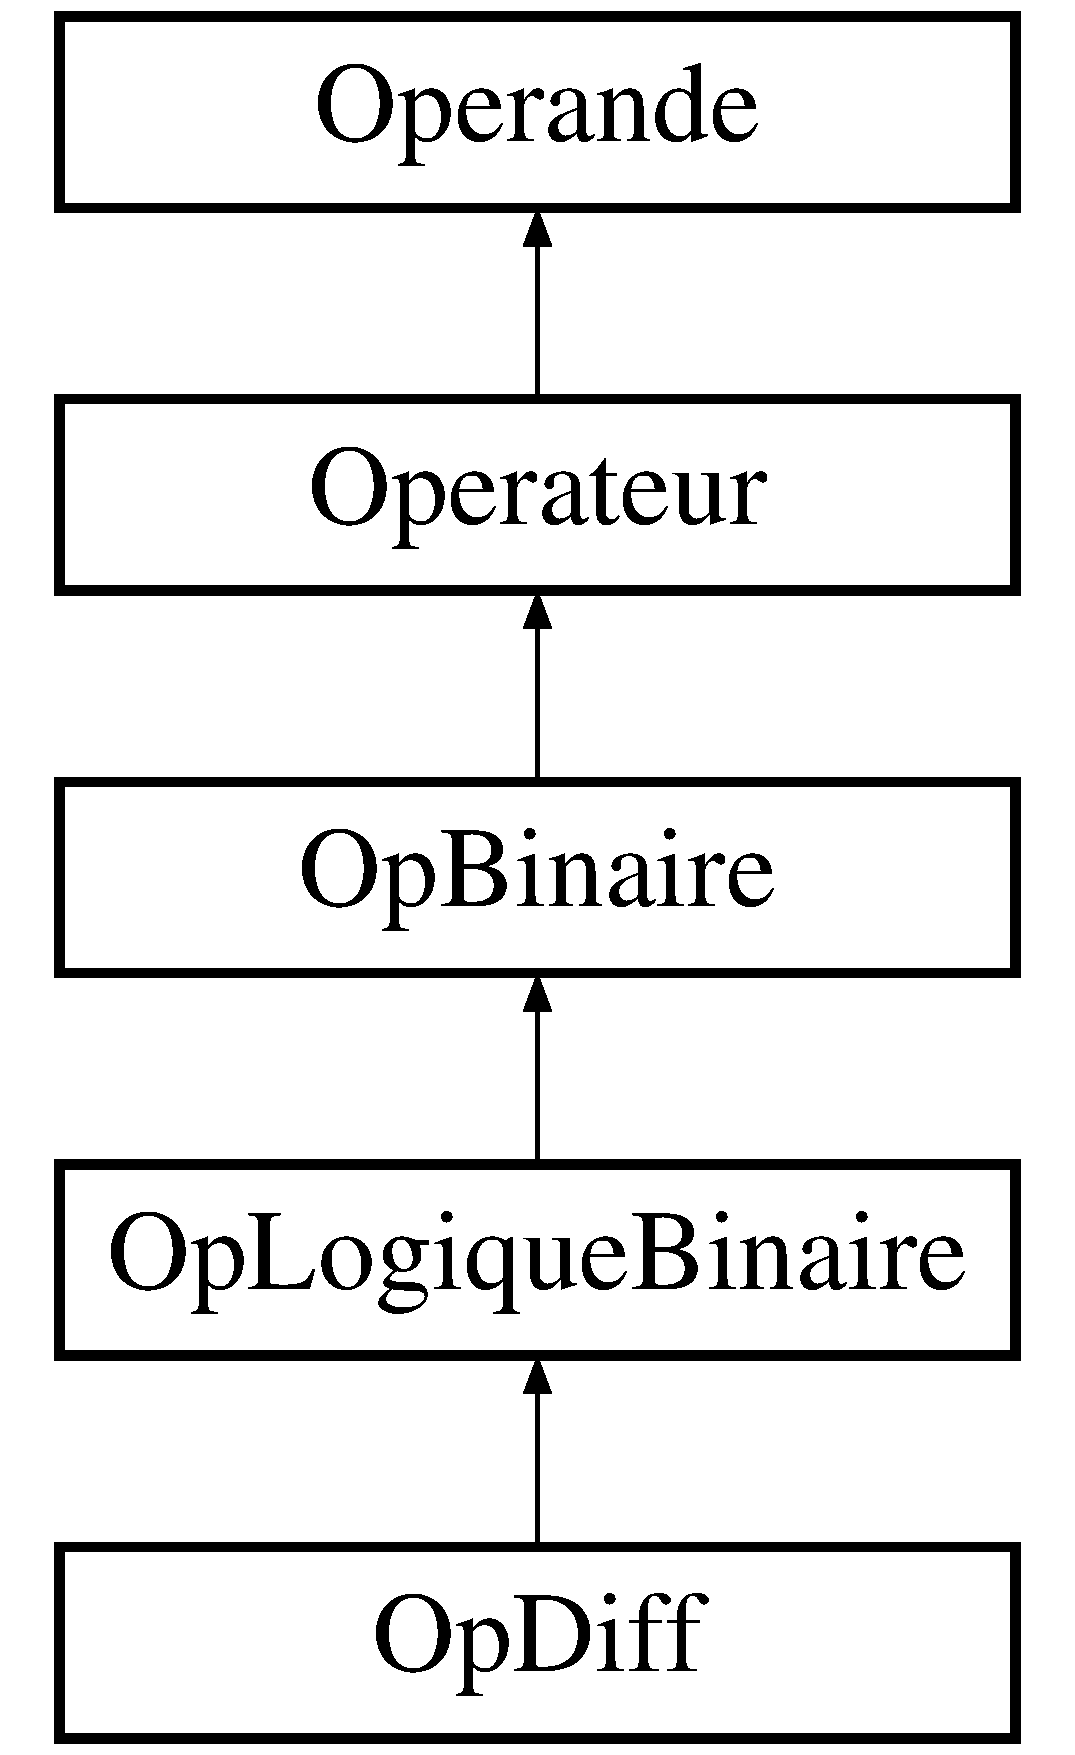
\includegraphics[height=5.000000cm]{class_op_diff}
\end{center}
\end{figure}
\subsection*{Public Member Functions}
\begin{DoxyCompactItemize}
\item 
\hyperlink{class_op_diff_a33196a59aff283870644fac58c81b82a}{Op\+Diff} ()
\item 
\hyperlink{class_litterale}{Litterale} $\ast$ \hyperlink{class_op_diff_aa863ce6389c18a0546f6b1b6aae4d9dd}{action\+Logi\+Numerique} (\hyperlink{class_lit_numerique}{Lit\+Numerique} $\ast$arg1, \hyperlink{class_lit_numerique}{Lit\+Numerique} $\ast$arg2)
\end{DoxyCompactItemize}
\subsection*{Additional Inherited Members}


\subsection{Detailed Description}


Definition at line 54 of file operator\+Logique.\+h.



\subsection{Constructor \& Destructor Documentation}
\index{Op\+Diff@{Op\+Diff}!Op\+Diff@{Op\+Diff}}
\index{Op\+Diff@{Op\+Diff}!Op\+Diff@{Op\+Diff}}
\subsubsection[{\texorpdfstring{Op\+Diff()}{OpDiff()}}]{\setlength{\rightskip}{0pt plus 5cm}Op\+Diff\+::\+Op\+Diff (
\begin{DoxyParamCaption}
{}
\end{DoxyParamCaption}
)\hspace{0.3cm}{\ttfamily [inline]}}\hypertarget{class_op_diff_a33196a59aff283870644fac58c81b82a}{}\label{class_op_diff_a33196a59aff283870644fac58c81b82a}


Definition at line 56 of file operator\+Logique.\+h.



\subsection{Member Function Documentation}
\index{Op\+Diff@{Op\+Diff}!action\+Logi\+Numerique@{action\+Logi\+Numerique}}
\index{action\+Logi\+Numerique@{action\+Logi\+Numerique}!Op\+Diff@{Op\+Diff}}
\subsubsection[{\texorpdfstring{action\+Logi\+Numerique(\+Lit\+Numerique $\ast$arg1, Lit\+Numerique $\ast$arg2)}{actionLogiNumerique(LitNumerique *arg1, LitNumerique *arg2)}}]{\setlength{\rightskip}{0pt plus 5cm}{\bf Litterale} $\ast$ Op\+Diff\+::action\+Logi\+Numerique (
\begin{DoxyParamCaption}
\item[{{\bf Lit\+Numerique} $\ast$}]{arg1, }
\item[{{\bf Lit\+Numerique} $\ast$}]{arg2}
\end{DoxyParamCaption}
)\hspace{0.3cm}{\ttfamily [virtual]}}\hypertarget{class_op_diff_aa863ce6389c18a0546f6b1b6aae4d9dd}{}\label{class_op_diff_aa863ce6389c18a0546f6b1b6aae4d9dd}


Implements \hyperlink{class_op_logique_binaire_a8fcab4c45ebcadbbcfecfa0c02e36f21}{Op\+Logique\+Binaire}.



Definition at line 44 of file operator\+Logique.\+cpp.



The documentation for this class was generated from the following files\+:\begin{DoxyCompactItemize}
\item 
\hyperlink{operator_logique_8h}{operator\+Logique.\+h}\item 
\hyperlink{operator_logique_8cpp}{operator\+Logique.\+cpp}\end{DoxyCompactItemize}

\hypertarget{class_op_dif_factory}{}\section{Op\+Dif\+Factory Class Reference}
\label{class_op_dif_factory}\index{Op\+Dif\+Factory@{Op\+Dif\+Factory}}


{\ttfamily \#include $<$operator\+Factory.\+h$>$}

Inheritance diagram for Op\+Dif\+Factory\+:\begin{figure}[H]
\begin{center}
\leavevmode
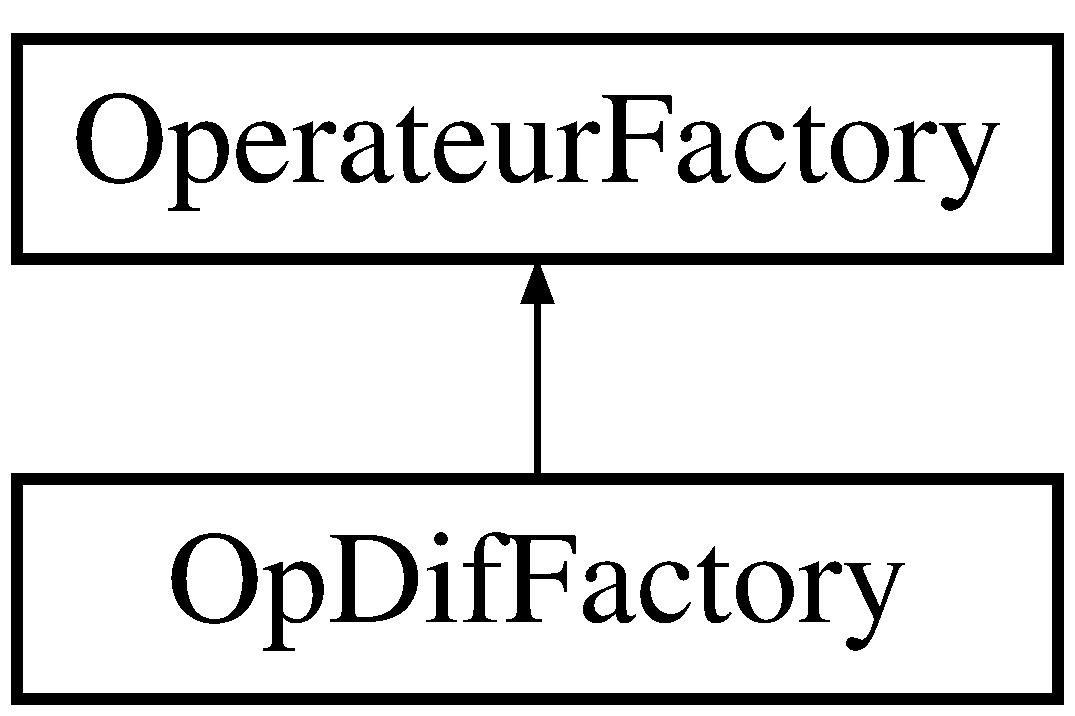
\includegraphics[height=2.000000cm]{class_op_dif_factory}
\end{center}
\end{figure}
\subsection*{Public Member Functions}
\begin{DoxyCompactItemize}
\item 
\hyperlink{class_op_dif_factory_aa25fab7d8ee5ac10f345993c24a6ae99}{Op\+Dif\+Factory} ()
\item 
\hyperlink{class_operateur}{Operateur} $\ast$ \hyperlink{class_op_dif_factory_af81849fc1a121fa627e7a17e60bed6bc}{get\+Operateur} ()
\end{DoxyCompactItemize}
\subsection*{Additional Inherited Members}


\subsection{Detailed Description}


Definition at line 246 of file operator\+Factory.\+h.



\subsection{Constructor \& Destructor Documentation}
\index{Op\+Dif\+Factory@{Op\+Dif\+Factory}!Op\+Dif\+Factory@{Op\+Dif\+Factory}}
\index{Op\+Dif\+Factory@{Op\+Dif\+Factory}!Op\+Dif\+Factory@{Op\+Dif\+Factory}}
\subsubsection[{\texorpdfstring{Op\+Dif\+Factory()}{OpDifFactory()}}]{\setlength{\rightskip}{0pt plus 5cm}Op\+Dif\+Factory\+::\+Op\+Dif\+Factory (
\begin{DoxyParamCaption}
{}
\end{DoxyParamCaption}
)\hspace{0.3cm}{\ttfamily [inline]}}\hypertarget{class_op_dif_factory_aa25fab7d8ee5ac10f345993c24a6ae99}{}\label{class_op_dif_factory_aa25fab7d8ee5ac10f345993c24a6ae99}


Definition at line 248 of file operator\+Factory.\+h.



\subsection{Member Function Documentation}
\index{Op\+Dif\+Factory@{Op\+Dif\+Factory}!get\+Operateur@{get\+Operateur}}
\index{get\+Operateur@{get\+Operateur}!Op\+Dif\+Factory@{Op\+Dif\+Factory}}
\subsubsection[{\texorpdfstring{get\+Operateur()}{getOperateur()}}]{\setlength{\rightskip}{0pt plus 5cm}{\bf Operateur}$\ast$ Op\+Dif\+Factory\+::get\+Operateur (
\begin{DoxyParamCaption}
{}
\end{DoxyParamCaption}
)\hspace{0.3cm}{\ttfamily [inline]}, {\ttfamily [virtual]}}\hypertarget{class_op_dif_factory_af81849fc1a121fa627e7a17e60bed6bc}{}\label{class_op_dif_factory_af81849fc1a121fa627e7a17e60bed6bc}


Implements \hyperlink{class_operateur_factory_aff61b2f67451f086d6abaea4231b2d78}{Operateur\+Factory}.



Definition at line 249 of file operator\+Factory.\+h.



The documentation for this class was generated from the following file\+:\begin{DoxyCompactItemize}
\item 
\hyperlink{operator_factory_8h}{operator\+Factory.\+h}\end{DoxyCompactItemize}

\hypertarget{class_op_div}{}\section{Op\+Div Class Reference}
\label{class_op_div}\index{Op\+Div@{Op\+Div}}


{\ttfamily \#include $<$operator\+Classique.\+h$>$}

Inheritance diagram for Op\+Div\+:\begin{figure}[H]
\begin{center}
\leavevmode
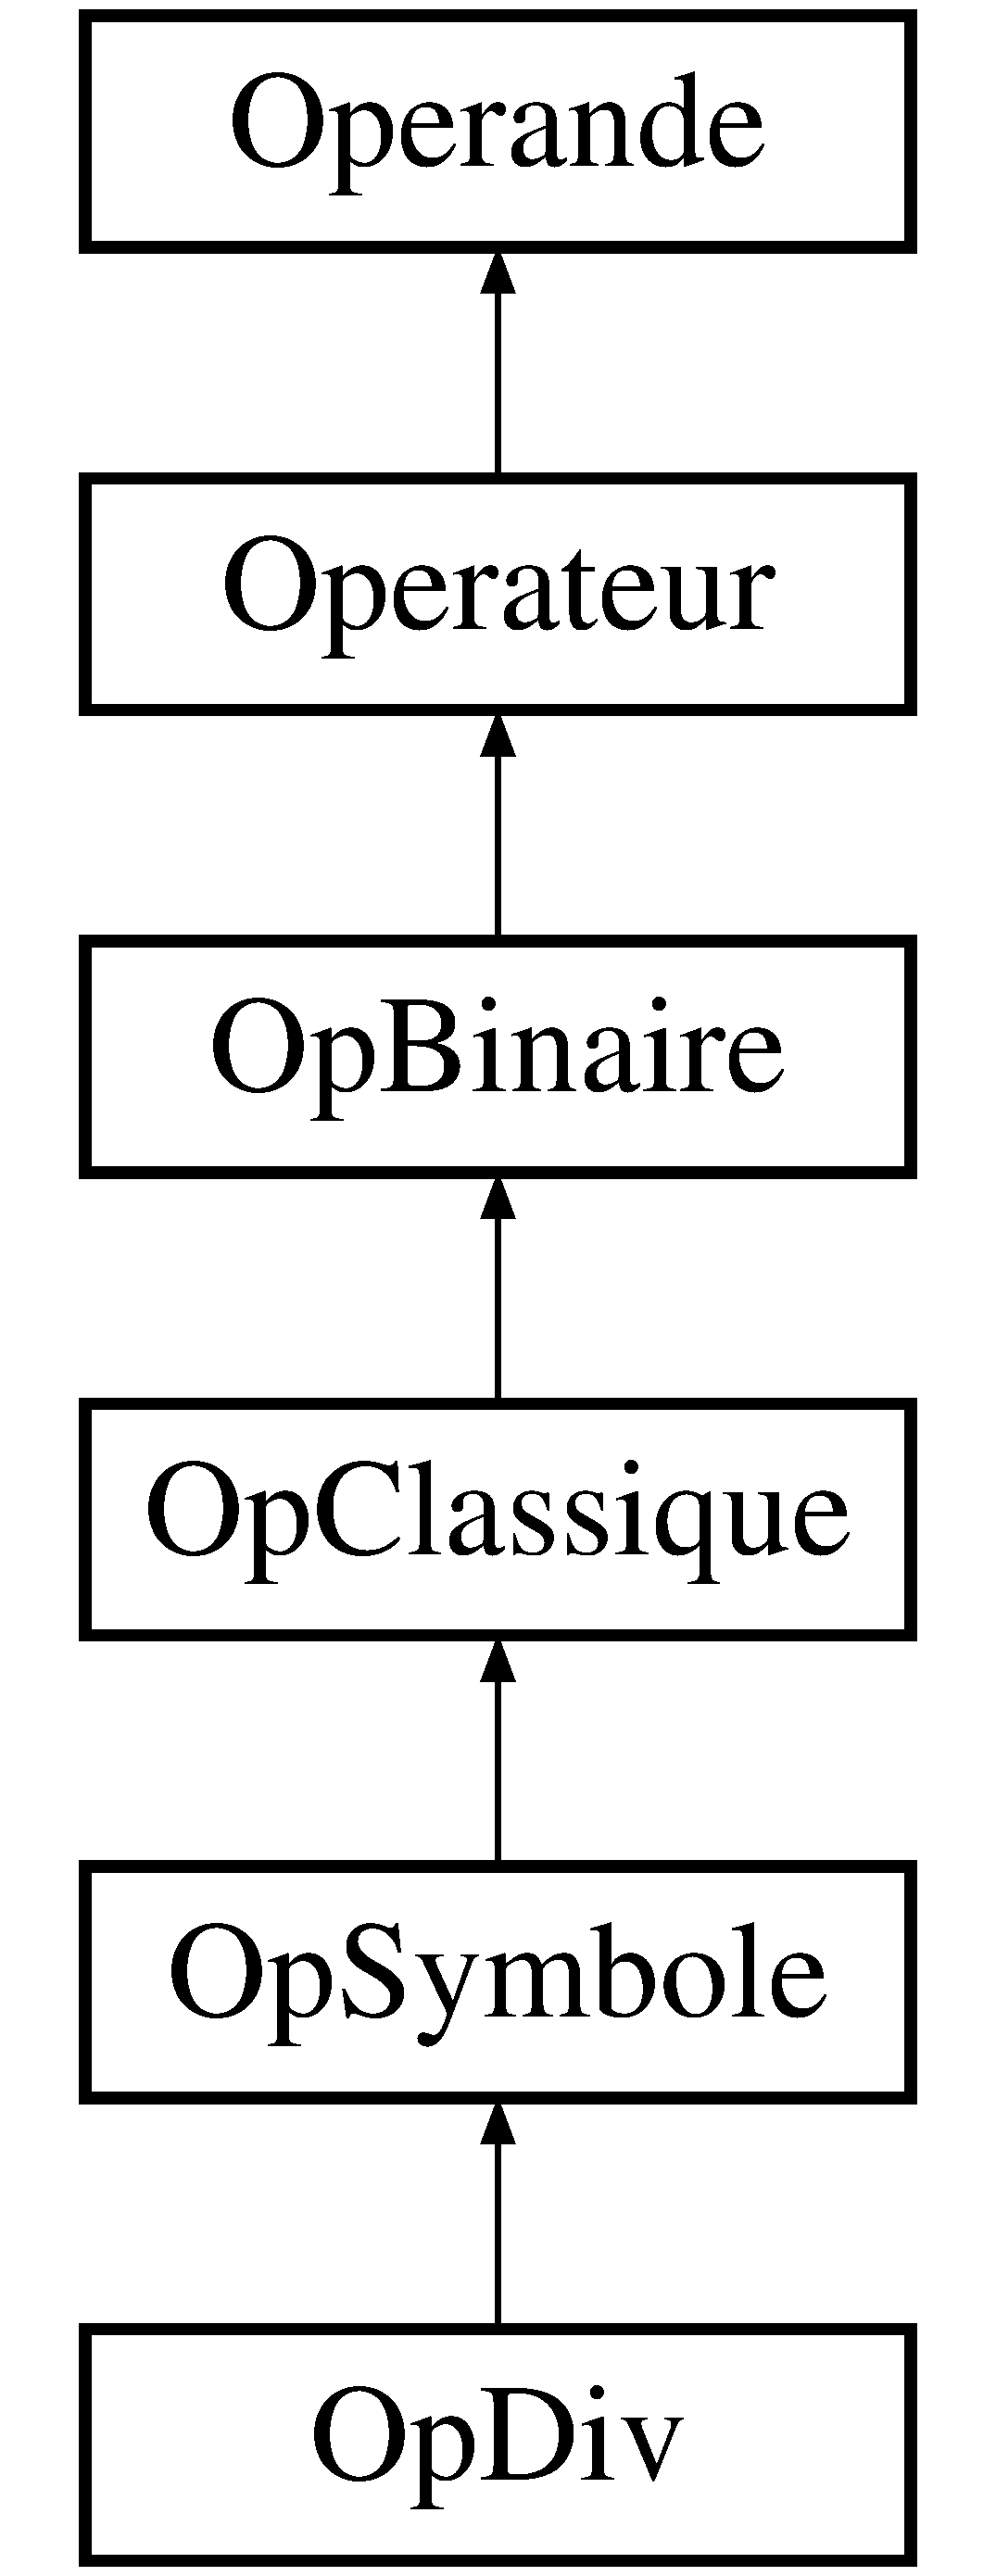
\includegraphics[height=6.000000cm]{class_op_div}
\end{center}
\end{figure}
\subsection*{Public Member Functions}
\begin{DoxyCompactItemize}
\item 
\hyperlink{class_op_div_a64f38b0d2adae50cbf651ada585810ea}{Op\+Div} ()
\item 
\hyperlink{class_litterale}{Litterale} $\ast$ \hyperlink{class_op_div_a2607c7a6356f4a3d358070b924e077ad}{fonction\+Num} (\hyperlink{class_nombres}{Nombres} $\ast$arg1, \hyperlink{class_litterale}{Litterale} $\ast$arg2)
\item 
\hyperlink{class_litterale}{Litterale} $\ast$ \hyperlink{class_op_div_acf1f9e49992b576d715c0bc0aaefaa24}{fonction\+Num2} (\hyperlink{class_entier}{Entier} $\ast$arg1, \hyperlink{class_litterale}{Litterale} $\ast$arg2)
\item 
\hyperlink{class_litterale}{Litterale} $\ast$ \hyperlink{class_op_div_a016aa0cfa3c8d176e515e78afed45a8a}{fonction\+Num2} (\hyperlink{class_reelle}{Reelle} $\ast$arg1, \hyperlink{class_litterale}{Litterale} $\ast$arg2)
\item 
\hyperlink{class_litterale}{Litterale} $\ast$ \hyperlink{class_op_div_a677140cc668980aa58768cf9517dd93e}{fonction\+Num2} (\hyperlink{class_rationnelle}{Rationnelle} $\ast$arg1, \hyperlink{class_litterale}{Litterale} $\ast$arg2)
\item 
\hyperlink{class_litterale}{Litterale} $\ast$ \hyperlink{class_op_div_a69b78b419ca90cfbd06c605130a5d0d1}{action\+Num} (\hyperlink{class_entier}{Entier} \&arg1, \hyperlink{class_entier}{Entier} \&arg2)
\item 
\hyperlink{class_litterale}{Litterale} $\ast$ \hyperlink{class_op_div_aa1de7148231747407140399b98fea6fc}{action\+Num} (\hyperlink{class_entier}{Entier} \&arg1, \hyperlink{class_reelle}{Reelle} \&arg2)
\item 
\hyperlink{class_litterale}{Litterale} $\ast$ \hyperlink{class_op_div_ae03a26237e3b8c8fe86e4f01b6daf2a6}{action\+Num} (\hyperlink{class_entier}{Entier} \&arg1, \hyperlink{class_rationnelle}{Rationnelle} \&arg2)
\item 
\hyperlink{class_litterale}{Litterale} $\ast$ \hyperlink{class_op_div_a7f38b0bb29be73d3b63404f5ae94c59f}{action\+Num} (\hyperlink{class_reelle}{Reelle} \&arg1, \hyperlink{class_reelle}{Reelle} \&arg2)
\item 
\hyperlink{class_litterale}{Litterale} $\ast$ \hyperlink{class_op_div_ab59aadcf7f16ef73877224e53467fc52}{action\+Num} (\hyperlink{class_reelle}{Reelle} \&arg1, \hyperlink{class_entier}{Entier} \&arg2)
\item 
\hyperlink{class_litterale}{Litterale} $\ast$ \hyperlink{class_op_div_a86afe5ae6bfddc41908d7c7017046c4c}{action\+Num} (\hyperlink{class_reelle}{Reelle} \&arg1, \hyperlink{class_rationnelle}{Rationnelle} \&arg2)
\item 
\hyperlink{class_litterale}{Litterale} $\ast$ \hyperlink{class_op_div_abc5e48f72857aff4a67941edbba48c2f}{action\+Num} (\hyperlink{class_rationnelle}{Rationnelle} \&arg1, \hyperlink{class_rationnelle}{Rationnelle} \&arg2)
\item 
\hyperlink{class_litterale}{Litterale} $\ast$ \hyperlink{class_op_div_a380c4447abba165dd42877b505811705}{action\+Num} (\hyperlink{class_rationnelle}{Rationnelle} \&arg1, \hyperlink{class_entier}{Entier} \&arg2)
\item 
\hyperlink{class_litterale}{Litterale} $\ast$ \hyperlink{class_op_div_a9ee9dc41c1f113d72bbd0af2522a6345}{action\+Num} (\hyperlink{class_rationnelle}{Rationnelle} \&arg1, \hyperlink{class_reelle}{Reelle} \&arg2)
\end{DoxyCompactItemize}
\subsection*{Additional Inherited Members}


\subsection{Detailed Description}


Definition at line 91 of file operator\+Classique.\+h.



\subsection{Constructor \& Destructor Documentation}
\index{Op\+Div@{Op\+Div}!Op\+Div@{Op\+Div}}
\index{Op\+Div@{Op\+Div}!Op\+Div@{Op\+Div}}
\subsubsection[{\texorpdfstring{Op\+Div()}{OpDiv()}}]{\setlength{\rightskip}{0pt plus 5cm}Op\+Div\+::\+Op\+Div (
\begin{DoxyParamCaption}
{}
\end{DoxyParamCaption}
)\hspace{0.3cm}{\ttfamily [inline]}}\hypertarget{class_op_div_a64f38b0d2adae50cbf651ada585810ea}{}\label{class_op_div_a64f38b0d2adae50cbf651ada585810ea}


Definition at line 93 of file operator\+Classique.\+h.



\subsection{Member Function Documentation}
\index{Op\+Div@{Op\+Div}!action\+Num@{action\+Num}}
\index{action\+Num@{action\+Num}!Op\+Div@{Op\+Div}}
\subsubsection[{\texorpdfstring{action\+Num(\+Entier \&arg1, Entier \&arg2)}{actionNum(Entier &arg1, Entier &arg2)}}]{\setlength{\rightskip}{0pt plus 5cm}{\bf Litterale} $\ast$ Op\+Div\+::action\+Num (
\begin{DoxyParamCaption}
\item[{{\bf Entier} \&}]{arg1, }
\item[{{\bf Entier} \&}]{arg2}
\end{DoxyParamCaption}
)\hspace{0.3cm}{\ttfamily [virtual]}}\hypertarget{class_op_div_a69b78b419ca90cfbd06c605130a5d0d1}{}\label{class_op_div_a69b78b419ca90cfbd06c605130a5d0d1}


Implements \hyperlink{class_op_symbole_a58c6b09cf3ccc1d753f6c5702eb3dfdd}{Op\+Symbole}.



Definition at line 306 of file operator\+Classique.\+cpp.

\index{Op\+Div@{Op\+Div}!action\+Num@{action\+Num}}
\index{action\+Num@{action\+Num}!Op\+Div@{Op\+Div}}
\subsubsection[{\texorpdfstring{action\+Num(\+Entier \&arg1, Reelle \&arg2)}{actionNum(Entier &arg1, Reelle &arg2)}}]{\setlength{\rightskip}{0pt plus 5cm}{\bf Litterale} $\ast$ Op\+Div\+::action\+Num (
\begin{DoxyParamCaption}
\item[{{\bf Entier} \&}]{arg1, }
\item[{{\bf Reelle} \&}]{arg2}
\end{DoxyParamCaption}
)\hspace{0.3cm}{\ttfamily [virtual]}}\hypertarget{class_op_div_aa1de7148231747407140399b98fea6fc}{}\label{class_op_div_aa1de7148231747407140399b98fea6fc}


Implements \hyperlink{class_op_symbole_a99b426017e9db00066ca7f960b7ab5aa}{Op\+Symbole}.



Definition at line 309 of file operator\+Classique.\+cpp.

\index{Op\+Div@{Op\+Div}!action\+Num@{action\+Num}}
\index{action\+Num@{action\+Num}!Op\+Div@{Op\+Div}}
\subsubsection[{\texorpdfstring{action\+Num(\+Entier \&arg1, Rationnelle \&arg2)}{actionNum(Entier &arg1, Rationnelle &arg2)}}]{\setlength{\rightskip}{0pt plus 5cm}{\bf Litterale} $\ast$ Op\+Div\+::action\+Num (
\begin{DoxyParamCaption}
\item[{{\bf Entier} \&}]{arg1, }
\item[{{\bf Rationnelle} \&}]{arg2}
\end{DoxyParamCaption}
)\hspace{0.3cm}{\ttfamily [virtual]}}\hypertarget{class_op_div_ae03a26237e3b8c8fe86e4f01b6daf2a6}{}\label{class_op_div_ae03a26237e3b8c8fe86e4f01b6daf2a6}


Implements \hyperlink{class_op_symbole_ae13989c55c53a7ec7c79d371ee05fbaa}{Op\+Symbole}.



Definition at line 312 of file operator\+Classique.\+cpp.

\index{Op\+Div@{Op\+Div}!action\+Num@{action\+Num}}
\index{action\+Num@{action\+Num}!Op\+Div@{Op\+Div}}
\subsubsection[{\texorpdfstring{action\+Num(\+Reelle \&arg1, Reelle \&arg2)}{actionNum(Reelle &arg1, Reelle &arg2)}}]{\setlength{\rightskip}{0pt plus 5cm}{\bf Litterale} $\ast$ Op\+Div\+::action\+Num (
\begin{DoxyParamCaption}
\item[{{\bf Reelle} \&}]{arg1, }
\item[{{\bf Reelle} \&}]{arg2}
\end{DoxyParamCaption}
)\hspace{0.3cm}{\ttfamily [virtual]}}\hypertarget{class_op_div_a7f38b0bb29be73d3b63404f5ae94c59f}{}\label{class_op_div_a7f38b0bb29be73d3b63404f5ae94c59f}


Implements \hyperlink{class_op_symbole_a98cfb6ae979dbe1974aa03387c682634}{Op\+Symbole}.



Definition at line 317 of file operator\+Classique.\+cpp.

\index{Op\+Div@{Op\+Div}!action\+Num@{action\+Num}}
\index{action\+Num@{action\+Num}!Op\+Div@{Op\+Div}}
\subsubsection[{\texorpdfstring{action\+Num(\+Reelle \&arg1, Entier \&arg2)}{actionNum(Reelle &arg1, Entier &arg2)}}]{\setlength{\rightskip}{0pt plus 5cm}{\bf Litterale} $\ast$ Op\+Div\+::action\+Num (
\begin{DoxyParamCaption}
\item[{{\bf Reelle} \&}]{arg1, }
\item[{{\bf Entier} \&}]{arg2}
\end{DoxyParamCaption}
)\hspace{0.3cm}{\ttfamily [virtual]}}\hypertarget{class_op_div_ab59aadcf7f16ef73877224e53467fc52}{}\label{class_op_div_ab59aadcf7f16ef73877224e53467fc52}


Implements \hyperlink{class_op_symbole_abfa9f422620f4fceaa18e5295b4c5b99}{Op\+Symbole}.



Definition at line 320 of file operator\+Classique.\+cpp.

\index{Op\+Div@{Op\+Div}!action\+Num@{action\+Num}}
\index{action\+Num@{action\+Num}!Op\+Div@{Op\+Div}}
\subsubsection[{\texorpdfstring{action\+Num(\+Reelle \&arg1, Rationnelle \&arg2)}{actionNum(Reelle &arg1, Rationnelle &arg2)}}]{\setlength{\rightskip}{0pt plus 5cm}{\bf Litterale} $\ast$ Op\+Div\+::action\+Num (
\begin{DoxyParamCaption}
\item[{{\bf Reelle} \&}]{arg1, }
\item[{{\bf Rationnelle} \&}]{arg2}
\end{DoxyParamCaption}
)\hspace{0.3cm}{\ttfamily [virtual]}}\hypertarget{class_op_div_a86afe5ae6bfddc41908d7c7017046c4c}{}\label{class_op_div_a86afe5ae6bfddc41908d7c7017046c4c}


Implements \hyperlink{class_op_symbole_a184453513af4b3146e753520f1ee760f}{Op\+Symbole}.



Definition at line 323 of file operator\+Classique.\+cpp.

\index{Op\+Div@{Op\+Div}!action\+Num@{action\+Num}}
\index{action\+Num@{action\+Num}!Op\+Div@{Op\+Div}}
\subsubsection[{\texorpdfstring{action\+Num(\+Rationnelle \&arg1, Rationnelle \&arg2)}{actionNum(Rationnelle &arg1, Rationnelle &arg2)}}]{\setlength{\rightskip}{0pt plus 5cm}{\bf Litterale} $\ast$ Op\+Div\+::action\+Num (
\begin{DoxyParamCaption}
\item[{{\bf Rationnelle} \&}]{arg1, }
\item[{{\bf Rationnelle} \&}]{arg2}
\end{DoxyParamCaption}
)\hspace{0.3cm}{\ttfamily [virtual]}}\hypertarget{class_op_div_abc5e48f72857aff4a67941edbba48c2f}{}\label{class_op_div_abc5e48f72857aff4a67941edbba48c2f}


Implements \hyperlink{class_op_symbole_ae63c8a614a14f75547919636e38c0901}{Op\+Symbole}.



Definition at line 327 of file operator\+Classique.\+cpp.

\index{Op\+Div@{Op\+Div}!action\+Num@{action\+Num}}
\index{action\+Num@{action\+Num}!Op\+Div@{Op\+Div}}
\subsubsection[{\texorpdfstring{action\+Num(\+Rationnelle \&arg1, Entier \&arg2)}{actionNum(Rationnelle &arg1, Entier &arg2)}}]{\setlength{\rightskip}{0pt plus 5cm}{\bf Litterale} $\ast$ Op\+Div\+::action\+Num (
\begin{DoxyParamCaption}
\item[{{\bf Rationnelle} \&}]{arg1, }
\item[{{\bf Entier} \&}]{arg2}
\end{DoxyParamCaption}
)\hspace{0.3cm}{\ttfamily [virtual]}}\hypertarget{class_op_div_a380c4447abba165dd42877b505811705}{}\label{class_op_div_a380c4447abba165dd42877b505811705}


Implements \hyperlink{class_op_symbole_adcacf42cf2baf8d96c0997f28d546d8e}{Op\+Symbole}.



Definition at line 332 of file operator\+Classique.\+cpp.

\index{Op\+Div@{Op\+Div}!action\+Num@{action\+Num}}
\index{action\+Num@{action\+Num}!Op\+Div@{Op\+Div}}
\subsubsection[{\texorpdfstring{action\+Num(\+Rationnelle \&arg1, Reelle \&arg2)}{actionNum(Rationnelle &arg1, Reelle &arg2)}}]{\setlength{\rightskip}{0pt plus 5cm}{\bf Litterale} $\ast$ Op\+Div\+::action\+Num (
\begin{DoxyParamCaption}
\item[{{\bf Rationnelle} \&}]{arg1, }
\item[{{\bf Reelle} \&}]{arg2}
\end{DoxyParamCaption}
)\hspace{0.3cm}{\ttfamily [virtual]}}\hypertarget{class_op_div_a9ee9dc41c1f113d72bbd0af2522a6345}{}\label{class_op_div_a9ee9dc41c1f113d72bbd0af2522a6345}


Implements \hyperlink{class_op_symbole_a031f540060b0744e7d2fa781a505e854}{Op\+Symbole}.



Definition at line 337 of file operator\+Classique.\+cpp.

\index{Op\+Div@{Op\+Div}!fonction\+Num@{fonction\+Num}}
\index{fonction\+Num@{fonction\+Num}!Op\+Div@{Op\+Div}}
\subsubsection[{\texorpdfstring{fonction\+Num(\+Nombres $\ast$arg1, Litterale $\ast$arg2)}{fonctionNum(Nombres *arg1, Litterale *arg2)}}]{\setlength{\rightskip}{0pt plus 5cm}{\bf Litterale} $\ast$ Op\+Div\+::fonction\+Num (
\begin{DoxyParamCaption}
\item[{{\bf Nombres} $\ast$}]{arg1, }
\item[{{\bf Litterale} $\ast$}]{arg2}
\end{DoxyParamCaption}
)\hspace{0.3cm}{\ttfamily [virtual]}}\hypertarget{class_op_div_a2607c7a6356f4a3d358070b924e077ad}{}\label{class_op_div_a2607c7a6356f4a3d358070b924e077ad}


Reimplemented from \hyperlink{class_op_symbole_ae908fd3da24f9cc8aa93f87360e07009}{Op\+Symbole}.



Definition at line 272 of file operator\+Classique.\+cpp.

\index{Op\+Div@{Op\+Div}!fonction\+Num2@{fonction\+Num2}}
\index{fonction\+Num2@{fonction\+Num2}!Op\+Div@{Op\+Div}}
\subsubsection[{\texorpdfstring{fonction\+Num2(\+Entier $\ast$arg1, Litterale $\ast$arg2)}{fonctionNum2(Entier *arg1, Litterale *arg2)}}]{\setlength{\rightskip}{0pt plus 5cm}{\bf Litterale} $\ast$ Op\+Div\+::fonction\+Num2 (
\begin{DoxyParamCaption}
\item[{{\bf Entier} $\ast$}]{arg1, }
\item[{{\bf Litterale} $\ast$}]{arg2}
\end{DoxyParamCaption}
)\hspace{0.3cm}{\ttfamily [virtual]}}\hypertarget{class_op_div_acf1f9e49992b576d715c0bc0aaefaa24}{}\label{class_op_div_acf1f9e49992b576d715c0bc0aaefaa24}


Reimplemented from \hyperlink{class_op_symbole_a69e1f5709d9ffba309d094856252eca7}{Op\+Symbole}.



Definition at line 278 of file operator\+Classique.\+cpp.

\index{Op\+Div@{Op\+Div}!fonction\+Num2@{fonction\+Num2}}
\index{fonction\+Num2@{fonction\+Num2}!Op\+Div@{Op\+Div}}
\subsubsection[{\texorpdfstring{fonction\+Num2(\+Reelle $\ast$arg1, Litterale $\ast$arg2)}{fonctionNum2(Reelle *arg1, Litterale *arg2)}}]{\setlength{\rightskip}{0pt plus 5cm}{\bf Litterale} $\ast$ Op\+Div\+::fonction\+Num2 (
\begin{DoxyParamCaption}
\item[{{\bf Reelle} $\ast$}]{arg1, }
\item[{{\bf Litterale} $\ast$}]{arg2}
\end{DoxyParamCaption}
)\hspace{0.3cm}{\ttfamily [virtual]}}\hypertarget{class_op_div_a016aa0cfa3c8d176e515e78afed45a8a}{}\label{class_op_div_a016aa0cfa3c8d176e515e78afed45a8a}


Reimplemented from \hyperlink{class_op_symbole_adacb4ef49ad6f19403a12b91ecb0c0f1}{Op\+Symbole}.



Definition at line 287 of file operator\+Classique.\+cpp.

\index{Op\+Div@{Op\+Div}!fonction\+Num2@{fonction\+Num2}}
\index{fonction\+Num2@{fonction\+Num2}!Op\+Div@{Op\+Div}}
\subsubsection[{\texorpdfstring{fonction\+Num2(\+Rationnelle $\ast$arg1, Litterale $\ast$arg2)}{fonctionNum2(Rationnelle *arg1, Litterale *arg2)}}]{\setlength{\rightskip}{0pt plus 5cm}{\bf Litterale} $\ast$ Op\+Div\+::fonction\+Num2 (
\begin{DoxyParamCaption}
\item[{{\bf Rationnelle} $\ast$}]{arg1, }
\item[{{\bf Litterale} $\ast$}]{arg2}
\end{DoxyParamCaption}
)\hspace{0.3cm}{\ttfamily [virtual]}}\hypertarget{class_op_div_a677140cc668980aa58768cf9517dd93e}{}\label{class_op_div_a677140cc668980aa58768cf9517dd93e}


Reimplemented from \hyperlink{class_op_symbole_a20ab54596cc3f3c8cdd059e13dc51541}{Op\+Symbole}.



Definition at line 296 of file operator\+Classique.\+cpp.



The documentation for this class was generated from the following files\+:\begin{DoxyCompactItemize}
\item 
\hyperlink{operator_classique_8h}{operator\+Classique.\+h}\item 
\hyperlink{operator_classique_8cpp}{operator\+Classique.\+cpp}\end{DoxyCompactItemize}

\hypertarget{class_op_div_factory}{}\section{Op\+Div\+Factory Class Reference}
\label{class_op_div_factory}\index{Op\+Div\+Factory@{Op\+Div\+Factory}}


{\ttfamily \#include $<$operator\+Factory.\+h$>$}

Inheritance diagram for Op\+Div\+Factory\+:\begin{figure}[H]
\begin{center}
\leavevmode
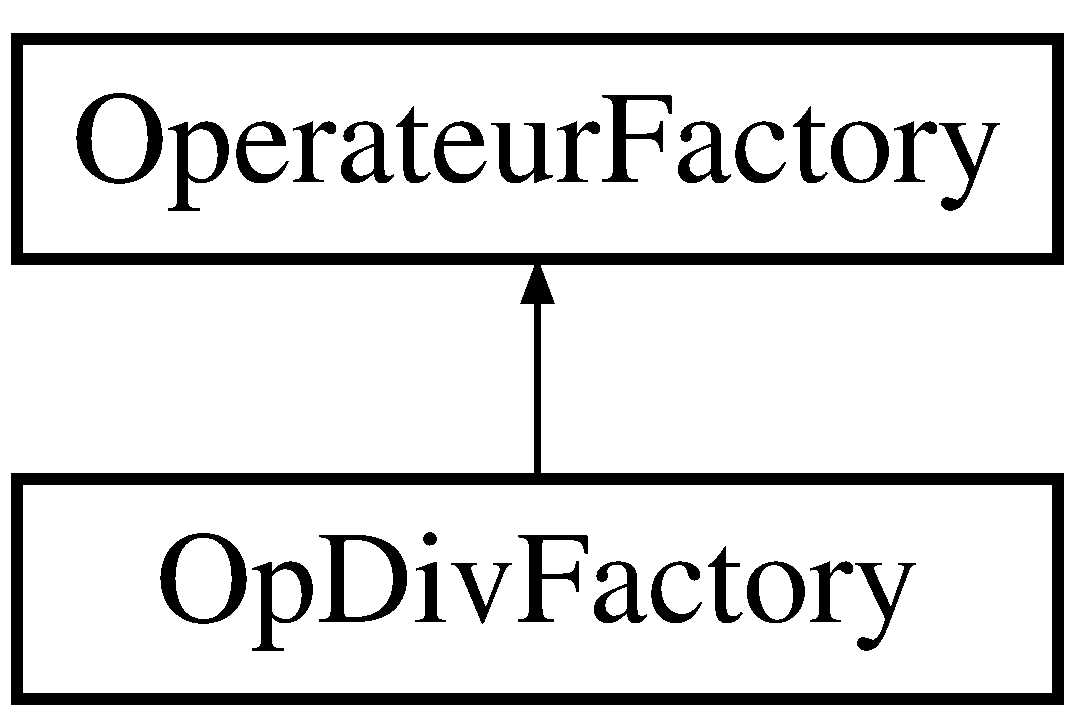
\includegraphics[height=2.000000cm]{class_op_div_factory}
\end{center}
\end{figure}
\subsection*{Public Member Functions}
\begin{DoxyCompactItemize}
\item 
\hyperlink{class_op_div_factory_a000c8f8093634e9877df3f299e57133e}{Op\+Div\+Factory} ()
\item 
\hyperlink{class_operateur}{Operateur} $\ast$ \hyperlink{class_op_div_factory_a6bb0a4145ccbafdc3f8016c85bff7be6}{get\+Operateur} ()
\end{DoxyCompactItemize}
\subsection*{Additional Inherited Members}


\subsection{Detailed Description}


Definition at line 210 of file operator\+Factory.\+h.



\subsection{Constructor \& Destructor Documentation}
\index{Op\+Div\+Factory@{Op\+Div\+Factory}!Op\+Div\+Factory@{Op\+Div\+Factory}}
\index{Op\+Div\+Factory@{Op\+Div\+Factory}!Op\+Div\+Factory@{Op\+Div\+Factory}}
\subsubsection[{\texorpdfstring{Op\+Div\+Factory()}{OpDivFactory()}}]{\setlength{\rightskip}{0pt plus 5cm}Op\+Div\+Factory\+::\+Op\+Div\+Factory (
\begin{DoxyParamCaption}
{}
\end{DoxyParamCaption}
)\hspace{0.3cm}{\ttfamily [inline]}}\hypertarget{class_op_div_factory_a000c8f8093634e9877df3f299e57133e}{}\label{class_op_div_factory_a000c8f8093634e9877df3f299e57133e}


Definition at line 212 of file operator\+Factory.\+h.



\subsection{Member Function Documentation}
\index{Op\+Div\+Factory@{Op\+Div\+Factory}!get\+Operateur@{get\+Operateur}}
\index{get\+Operateur@{get\+Operateur}!Op\+Div\+Factory@{Op\+Div\+Factory}}
\subsubsection[{\texorpdfstring{get\+Operateur()}{getOperateur()}}]{\setlength{\rightskip}{0pt plus 5cm}{\bf Operateur}$\ast$ Op\+Div\+Factory\+::get\+Operateur (
\begin{DoxyParamCaption}
{}
\end{DoxyParamCaption}
)\hspace{0.3cm}{\ttfamily [inline]}, {\ttfamily [virtual]}}\hypertarget{class_op_div_factory_a6bb0a4145ccbafdc3f8016c85bff7be6}{}\label{class_op_div_factory_a6bb0a4145ccbafdc3f8016c85bff7be6}


Implements \hyperlink{class_operateur_factory_aff61b2f67451f086d6abaea4231b2d78}{Operateur\+Factory}.



Definition at line 213 of file operator\+Factory.\+h.



The documentation for this class was generated from the following file\+:\begin{DoxyCompactItemize}
\item 
\hyperlink{operator_factory_8h}{operator\+Factory.\+h}\end{DoxyCompactItemize}

\hypertarget{class_op_drop}{}\section{Op\+Drop Class Reference}
\label{class_op_drop}\index{Op\+Drop@{Op\+Drop}}


{\ttfamily \#include $<$operator.\+h$>$}

Inheritance diagram for Op\+Drop\+:\begin{figure}[H]
\begin{center}
\leavevmode
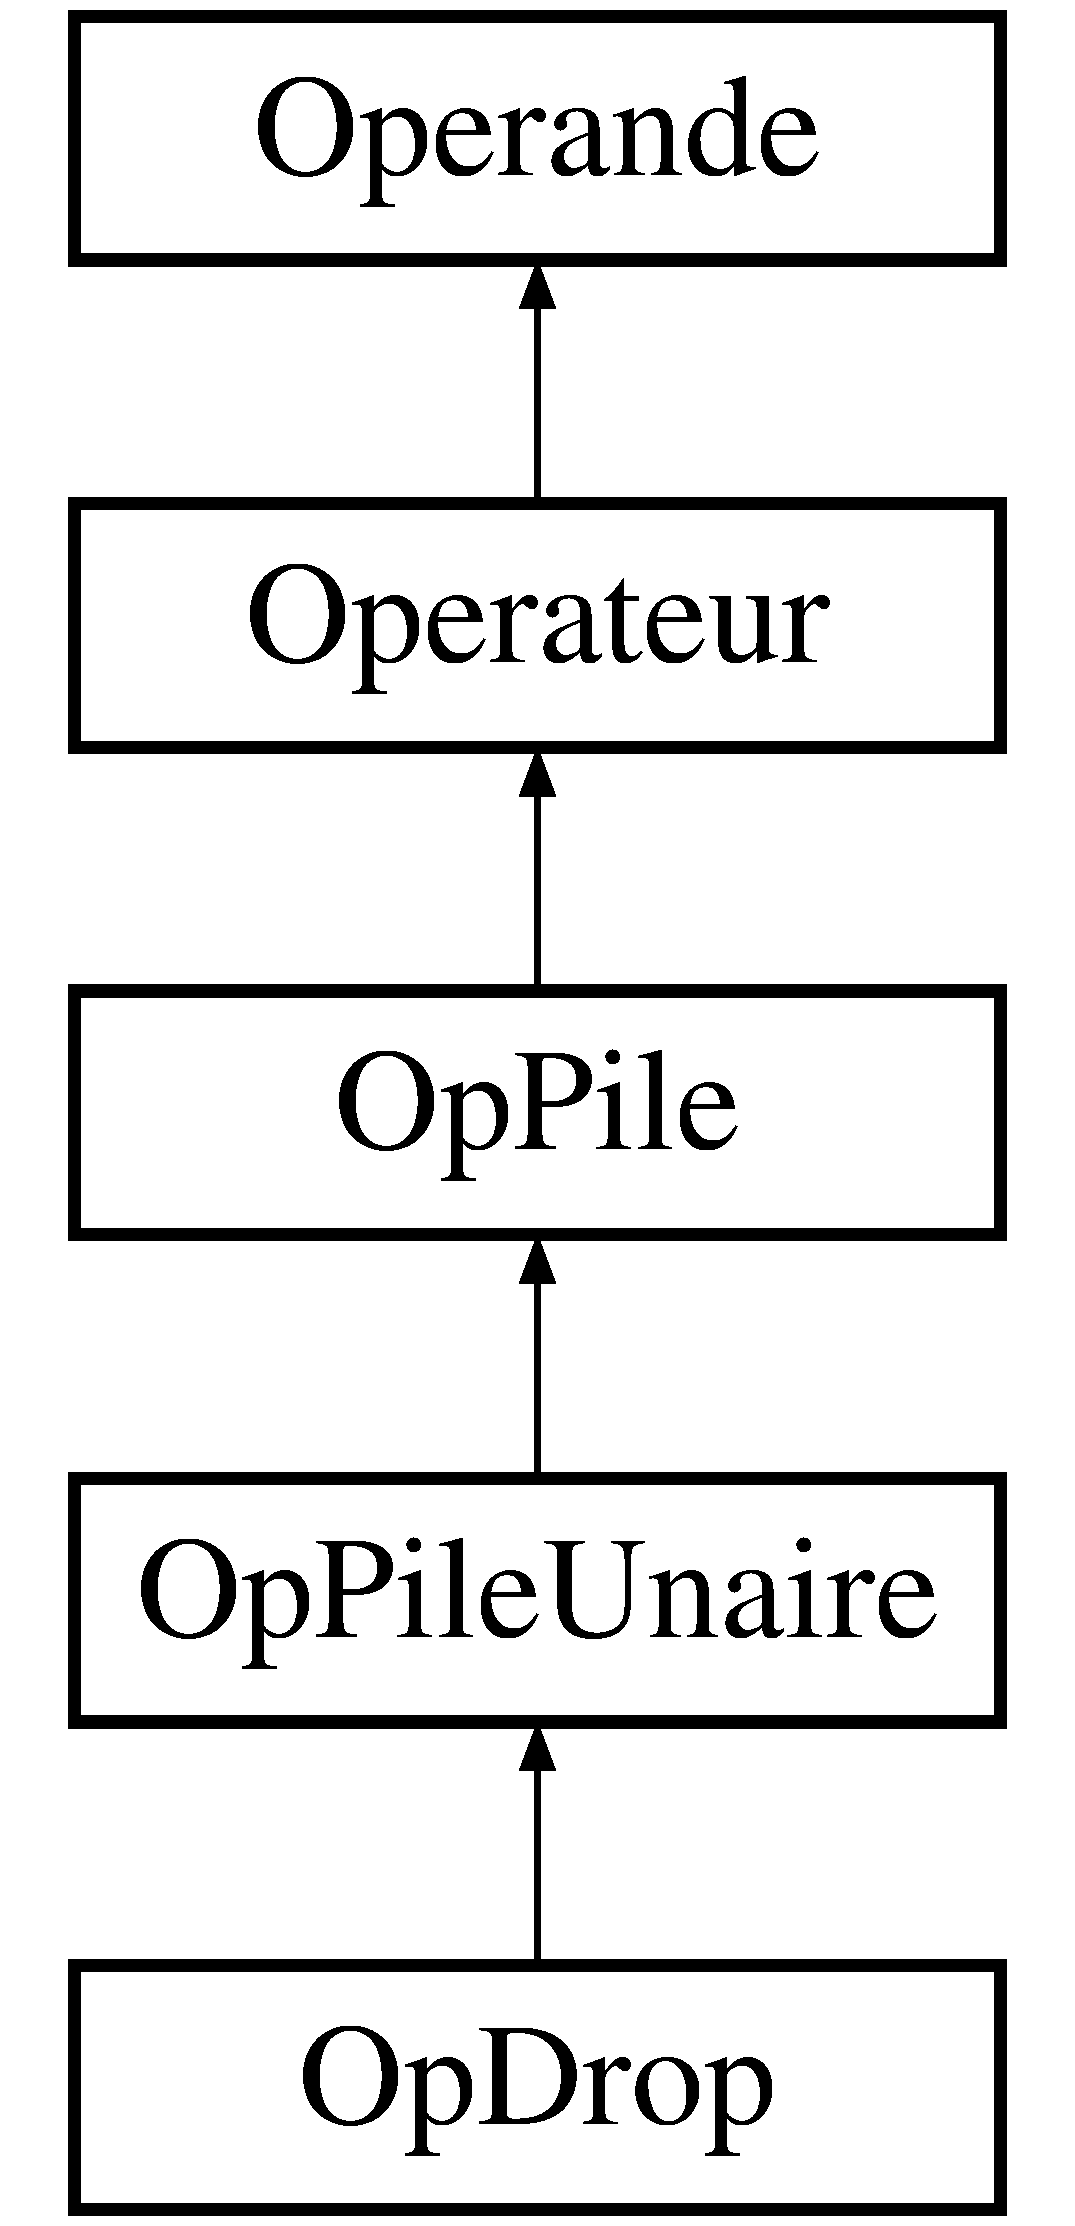
\includegraphics[height=5.000000cm]{class_op_drop}
\end{center}
\end{figure}
\subsection*{Public Member Functions}
\begin{DoxyCompactItemize}
\item 
\hyperlink{class_op_drop_acc20813c444d2da5f7bcecce2c7784e0}{Op\+Drop} ()
\item 
void \hyperlink{class_op_drop_a4d898f75bf84b66c315711af17f4eda7}{executer\+Pile} ()
\end{DoxyCompactItemize}
\subsection*{Additional Inherited Members}


\subsection{Detailed Description}


Definition at line 233 of file operator.\+h.



\subsection{Constructor \& Destructor Documentation}
\index{Op\+Drop@{Op\+Drop}!Op\+Drop@{Op\+Drop}}
\index{Op\+Drop@{Op\+Drop}!Op\+Drop@{Op\+Drop}}
\subsubsection[{\texorpdfstring{Op\+Drop()}{OpDrop()}}]{\setlength{\rightskip}{0pt plus 5cm}Op\+Drop\+::\+Op\+Drop (
\begin{DoxyParamCaption}
{}
\end{DoxyParamCaption}
)\hspace{0.3cm}{\ttfamily [inline]}}\hypertarget{class_op_drop_acc20813c444d2da5f7bcecce2c7784e0}{}\label{class_op_drop_acc20813c444d2da5f7bcecce2c7784e0}


Definition at line 235 of file operator.\+h.



\subsection{Member Function Documentation}
\index{Op\+Drop@{Op\+Drop}!executer\+Pile@{executer\+Pile}}
\index{executer\+Pile@{executer\+Pile}!Op\+Drop@{Op\+Drop}}
\subsubsection[{\texorpdfstring{executer\+Pile()}{executerPile()}}]{\setlength{\rightskip}{0pt plus 5cm}void Op\+Drop\+::executer\+Pile (
\begin{DoxyParamCaption}
{}
\end{DoxyParamCaption}
)\hspace{0.3cm}{\ttfamily [virtual]}}\hypertarget{class_op_drop_a4d898f75bf84b66c315711af17f4eda7}{}\label{class_op_drop_a4d898f75bf84b66c315711af17f4eda7}


Reimplemented from \hyperlink{class_op_pile_unaire_ae7f0b928350431fd080150a89312f3cf}{Op\+Pile\+Unaire}.



Definition at line 277 of file operator.\+cpp.



The documentation for this class was generated from the following files\+:\begin{DoxyCompactItemize}
\item 
\hyperlink{operator_8h}{operator.\+h}\item 
\hyperlink{operator_8cpp}{operator.\+cpp}\end{DoxyCompactItemize}

\hypertarget{class_op_drop_factory}{}\section{Op\+Drop\+Factory Class Reference}
\label{class_op_drop_factory}\index{Op\+Drop\+Factory@{Op\+Drop\+Factory}}


{\ttfamily \#include $<$operator\+Factory.\+h$>$}

Inheritance diagram for Op\+Drop\+Factory\+:\begin{figure}[H]
\begin{center}
\leavevmode
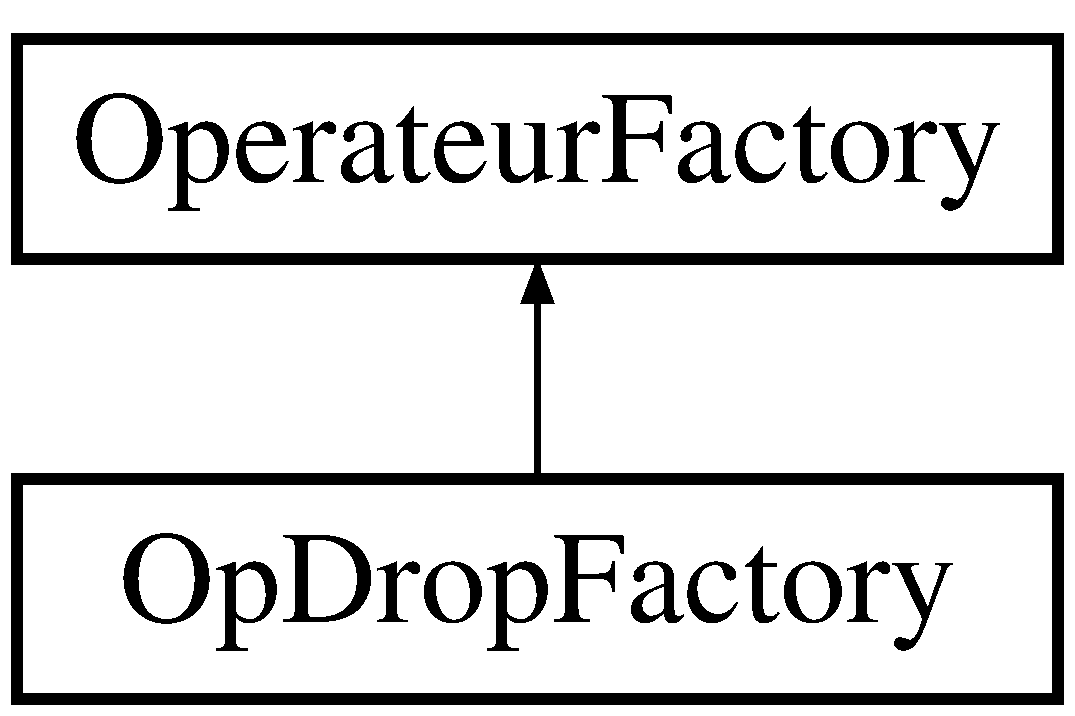
\includegraphics[height=2.000000cm]{class_op_drop_factory}
\end{center}
\end{figure}
\subsection*{Public Member Functions}
\begin{DoxyCompactItemize}
\item 
\hyperlink{class_op_drop_factory_ae6e407cdf88d9c13776875788fb904dc}{Op\+Drop\+Factory} ()
\item 
\hyperlink{class_operateur}{Operateur} $\ast$ \hyperlink{class_op_drop_factory_af8741d23a6de569d9997adcfb9410efb}{get\+Operateur} ()
\end{DoxyCompactItemize}
\subsection*{Additional Inherited Members}


\subsection{Detailed Description}


Definition at line 129 of file operator\+Factory.\+h.



\subsection{Constructor \& Destructor Documentation}
\index{Op\+Drop\+Factory@{Op\+Drop\+Factory}!Op\+Drop\+Factory@{Op\+Drop\+Factory}}
\index{Op\+Drop\+Factory@{Op\+Drop\+Factory}!Op\+Drop\+Factory@{Op\+Drop\+Factory}}
\subsubsection[{\texorpdfstring{Op\+Drop\+Factory()}{OpDropFactory()}}]{\setlength{\rightskip}{0pt plus 5cm}Op\+Drop\+Factory\+::\+Op\+Drop\+Factory (
\begin{DoxyParamCaption}
{}
\end{DoxyParamCaption}
)\hspace{0.3cm}{\ttfamily [inline]}}\hypertarget{class_op_drop_factory_ae6e407cdf88d9c13776875788fb904dc}{}\label{class_op_drop_factory_ae6e407cdf88d9c13776875788fb904dc}


Definition at line 131 of file operator\+Factory.\+h.



\subsection{Member Function Documentation}
\index{Op\+Drop\+Factory@{Op\+Drop\+Factory}!get\+Operateur@{get\+Operateur}}
\index{get\+Operateur@{get\+Operateur}!Op\+Drop\+Factory@{Op\+Drop\+Factory}}
\subsubsection[{\texorpdfstring{get\+Operateur()}{getOperateur()}}]{\setlength{\rightskip}{0pt plus 5cm}{\bf Operateur}$\ast$ Op\+Drop\+Factory\+::get\+Operateur (
\begin{DoxyParamCaption}
{}
\end{DoxyParamCaption}
)\hspace{0.3cm}{\ttfamily [inline]}, {\ttfamily [virtual]}}\hypertarget{class_op_drop_factory_af8741d23a6de569d9997adcfb9410efb}{}\label{class_op_drop_factory_af8741d23a6de569d9997adcfb9410efb}


Implements \hyperlink{class_operateur_factory_aff61b2f67451f086d6abaea4231b2d78}{Operateur\+Factory}.



Definition at line 132 of file operator\+Factory.\+h.



The documentation for this class was generated from the following file\+:\begin{DoxyCompactItemize}
\item 
\hyperlink{operator_factory_8h}{operator\+Factory.\+h}\end{DoxyCompactItemize}

\hypertarget{class_op_dup}{}\section{Op\+Dup Class Reference}
\label{class_op_dup}\index{Op\+Dup@{Op\+Dup}}


{\ttfamily \#include $<$operator.\+h$>$}

Inheritance diagram for Op\+Dup\+:\begin{figure}[H]
\begin{center}
\leavevmode
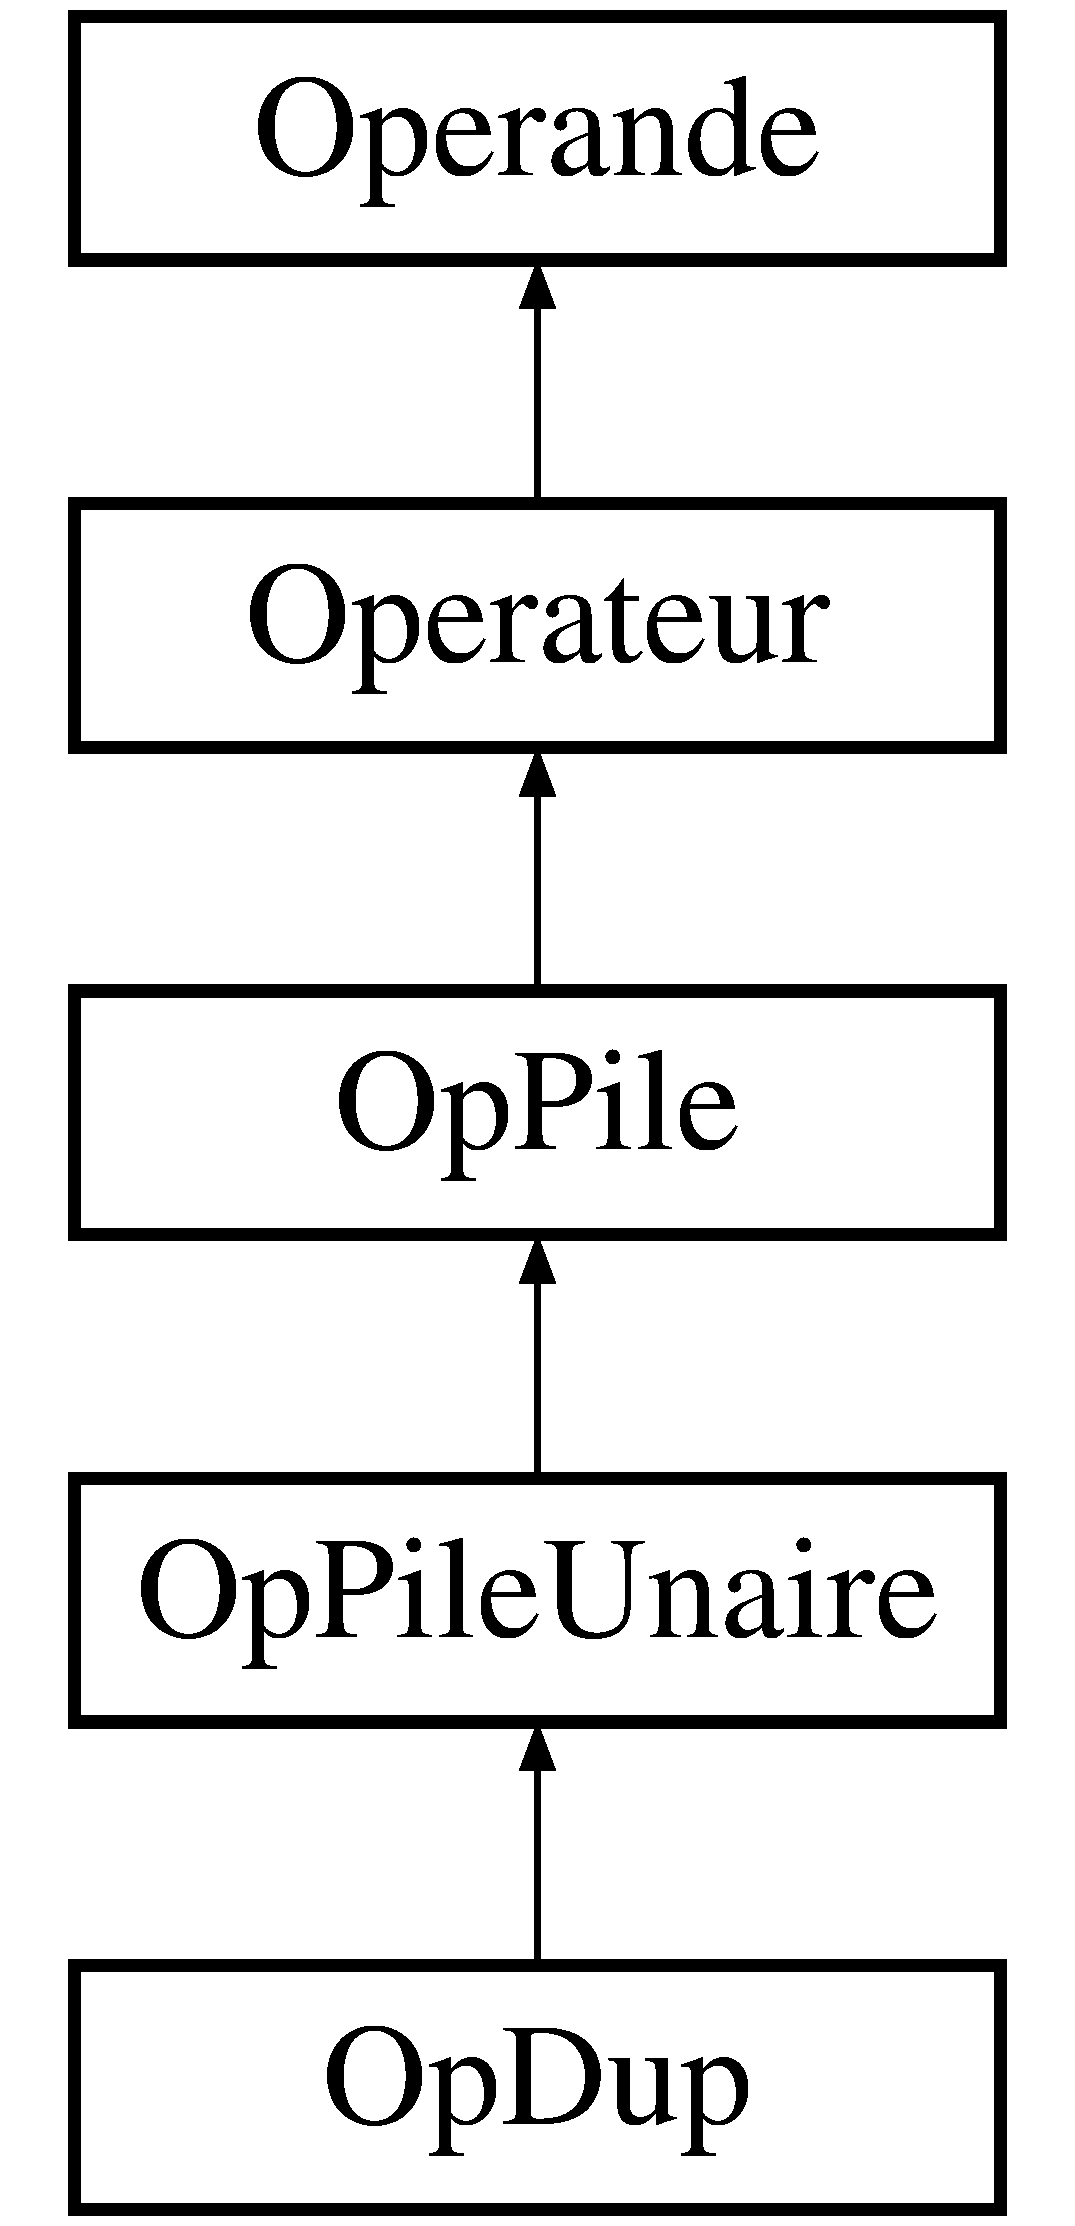
\includegraphics[height=5.000000cm]{class_op_dup}
\end{center}
\end{figure}
\subsection*{Public Member Functions}
\begin{DoxyCompactItemize}
\item 
\hyperlink{class_op_dup_a3e084c97c1c5d6b50ecc910a41fd5a15}{Op\+Dup} ()
\item 
void \hyperlink{class_op_dup_a74be123d0c6afffe5bdb3b7c0c5feefc}{executer\+Pile} ()
\item 
void \hyperlink{class_op_dup_af788cceb322772cf33e28aacfd922fc4}{fonction\+Num} (\hyperlink{class_litterale}{Litterale} $\ast$arg1)
\end{DoxyCompactItemize}
\subsection*{Additional Inherited Members}


\subsection{Detailed Description}


Definition at line 225 of file operator.\+h.



\subsection{Constructor \& Destructor Documentation}
\index{Op\+Dup@{Op\+Dup}!Op\+Dup@{Op\+Dup}}
\index{Op\+Dup@{Op\+Dup}!Op\+Dup@{Op\+Dup}}
\subsubsection[{\texorpdfstring{Op\+Dup()}{OpDup()}}]{\setlength{\rightskip}{0pt plus 5cm}Op\+Dup\+::\+Op\+Dup (
\begin{DoxyParamCaption}
{}
\end{DoxyParamCaption}
)\hspace{0.3cm}{\ttfamily [inline]}}\hypertarget{class_op_dup_a3e084c97c1c5d6b50ecc910a41fd5a15}{}\label{class_op_dup_a3e084c97c1c5d6b50ecc910a41fd5a15}


Definition at line 227 of file operator.\+h.



\subsection{Member Function Documentation}
\index{Op\+Dup@{Op\+Dup}!executer\+Pile@{executer\+Pile}}
\index{executer\+Pile@{executer\+Pile}!Op\+Dup@{Op\+Dup}}
\subsubsection[{\texorpdfstring{executer\+Pile()}{executerPile()}}]{\setlength{\rightskip}{0pt plus 5cm}void Op\+Dup\+::executer\+Pile (
\begin{DoxyParamCaption}
{}
\end{DoxyParamCaption}
)\hspace{0.3cm}{\ttfamily [virtual]}}\hypertarget{class_op_dup_a74be123d0c6afffe5bdb3b7c0c5feefc}{}\label{class_op_dup_a74be123d0c6afffe5bdb3b7c0c5feefc}


Reimplemented from \hyperlink{class_op_pile_unaire_ae7f0b928350431fd080150a89312f3cf}{Op\+Pile\+Unaire}.



Definition at line 273 of file operator.\+cpp.

\index{Op\+Dup@{Op\+Dup}!fonction\+Num@{fonction\+Num}}
\index{fonction\+Num@{fonction\+Num}!Op\+Dup@{Op\+Dup}}
\subsubsection[{\texorpdfstring{fonction\+Num(\+Litterale $\ast$arg1)}{fonctionNum(Litterale *arg1)}}]{\setlength{\rightskip}{0pt plus 5cm}void Op\+Dup\+::fonction\+Num (
\begin{DoxyParamCaption}
\item[{{\bf Litterale} $\ast$}]{arg1}
\end{DoxyParamCaption}
)}\hypertarget{class_op_dup_af788cceb322772cf33e28aacfd922fc4}{}\label{class_op_dup_af788cceb322772cf33e28aacfd922fc4}


The documentation for this class was generated from the following files\+:\begin{DoxyCompactItemize}
\item 
\hyperlink{operator_8h}{operator.\+h}\item 
\hyperlink{operator_8cpp}{operator.\+cpp}\end{DoxyCompactItemize}

\hypertarget{class_op_dup_factory}{}\section{Op\+Dup\+Factory Class Reference}
\label{class_op_dup_factory}\index{Op\+Dup\+Factory@{Op\+Dup\+Factory}}


{\ttfamily \#include $<$operator\+Factory.\+h$>$}

Inheritance diagram for Op\+Dup\+Factory\+:\begin{figure}[H]
\begin{center}
\leavevmode
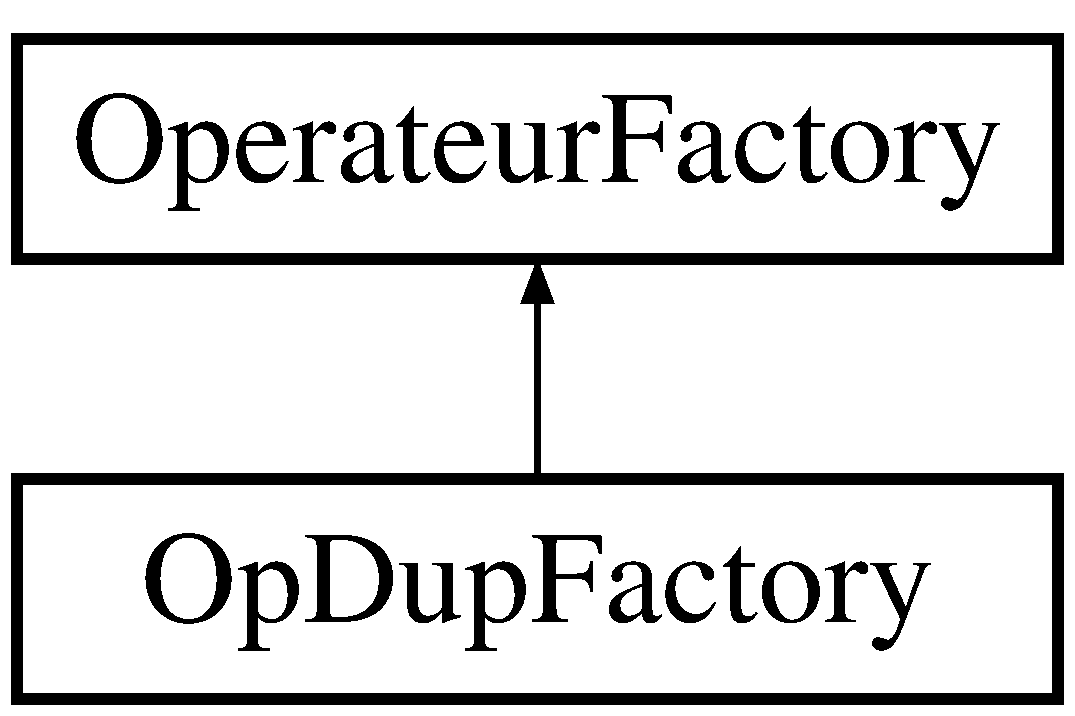
\includegraphics[height=2.000000cm]{class_op_dup_factory}
\end{center}
\end{figure}
\subsection*{Public Member Functions}
\begin{DoxyCompactItemize}
\item 
\hyperlink{class_op_dup_factory_adcf6d7fc0ec43967ac00331851348591}{Op\+Dup\+Factory} ()
\item 
\hyperlink{class_operateur}{Operateur} $\ast$ \hyperlink{class_op_dup_factory_a5e10a3addcdcfd660c13458408e78359}{get\+Operateur} ()
\end{DoxyCompactItemize}
\subsection*{Additional Inherited Members}


\subsection{Detailed Description}


Definition at line 123 of file operator\+Factory.\+h.



\subsection{Constructor \& Destructor Documentation}
\index{Op\+Dup\+Factory@{Op\+Dup\+Factory}!Op\+Dup\+Factory@{Op\+Dup\+Factory}}
\index{Op\+Dup\+Factory@{Op\+Dup\+Factory}!Op\+Dup\+Factory@{Op\+Dup\+Factory}}
\subsubsection[{\texorpdfstring{Op\+Dup\+Factory()}{OpDupFactory()}}]{\setlength{\rightskip}{0pt plus 5cm}Op\+Dup\+Factory\+::\+Op\+Dup\+Factory (
\begin{DoxyParamCaption}
{}
\end{DoxyParamCaption}
)\hspace{0.3cm}{\ttfamily [inline]}}\hypertarget{class_op_dup_factory_adcf6d7fc0ec43967ac00331851348591}{}\label{class_op_dup_factory_adcf6d7fc0ec43967ac00331851348591}


Definition at line 125 of file operator\+Factory.\+h.



\subsection{Member Function Documentation}
\index{Op\+Dup\+Factory@{Op\+Dup\+Factory}!get\+Operateur@{get\+Operateur}}
\index{get\+Operateur@{get\+Operateur}!Op\+Dup\+Factory@{Op\+Dup\+Factory}}
\subsubsection[{\texorpdfstring{get\+Operateur()}{getOperateur()}}]{\setlength{\rightskip}{0pt plus 5cm}{\bf Operateur}$\ast$ Op\+Dup\+Factory\+::get\+Operateur (
\begin{DoxyParamCaption}
{}
\end{DoxyParamCaption}
)\hspace{0.3cm}{\ttfamily [inline]}, {\ttfamily [virtual]}}\hypertarget{class_op_dup_factory_a5e10a3addcdcfd660c13458408e78359}{}\label{class_op_dup_factory_a5e10a3addcdcfd660c13458408e78359}


Implements \hyperlink{class_operateur_factory_aff61b2f67451f086d6abaea4231b2d78}{Operateur\+Factory}.



Definition at line 126 of file operator\+Factory.\+h.



The documentation for this class was generated from the following file\+:\begin{DoxyCompactItemize}
\item 
\hyperlink{operator_factory_8h}{operator\+Factory.\+h}\end{DoxyCompactItemize}

\hypertarget{class_op_eg}{}\section{Op\+Eg Class Reference}
\label{class_op_eg}\index{Op\+Eg@{Op\+Eg}}


{\ttfamily \#include $<$operator\+Logique.\+h$>$}

Inheritance diagram for Op\+Eg\+:\begin{figure}[H]
\begin{center}
\leavevmode
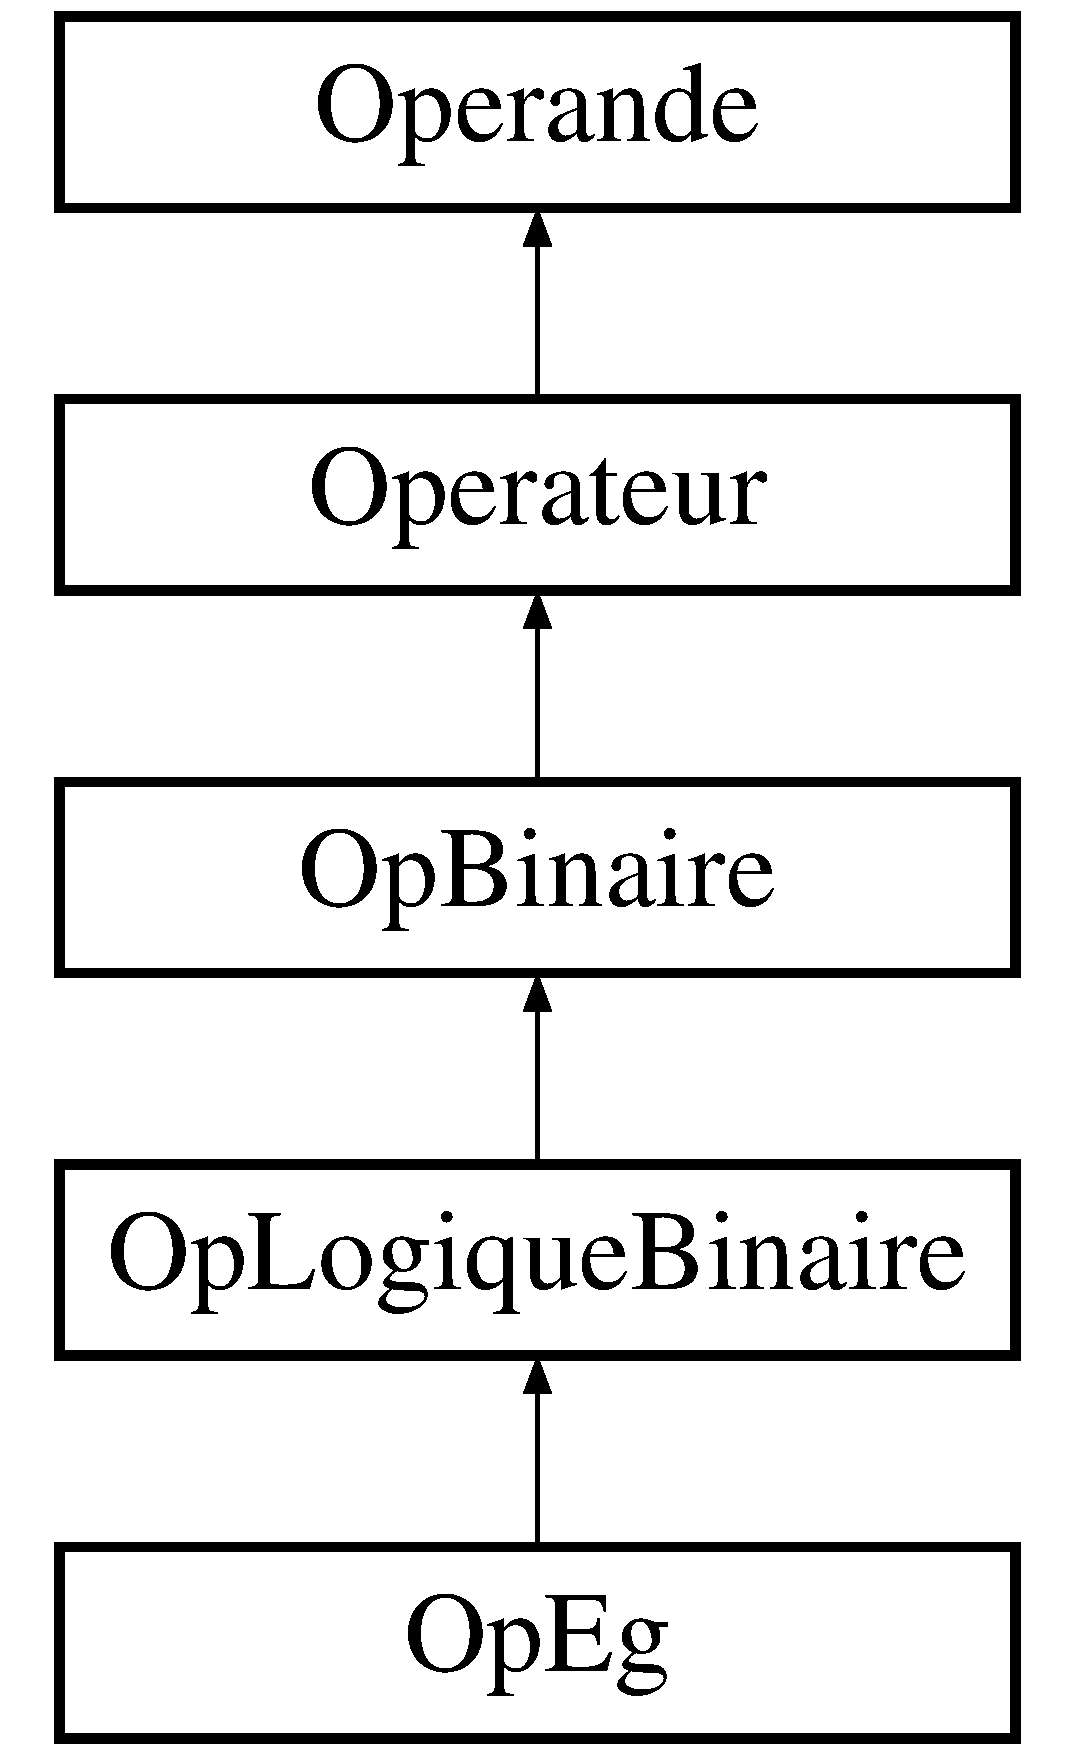
\includegraphics[height=5.000000cm]{class_op_eg}
\end{center}
\end{figure}
\subsection*{Public Member Functions}
\begin{DoxyCompactItemize}
\item 
\hyperlink{class_op_eg_ae968a0218a21104fcc74ccb24518619c}{Op\+Eg} ()
\item 
\hyperlink{class_litterale}{Litterale} $\ast$ \hyperlink{class_op_eg_ab84762131924ea6ca5e60960593411e0}{action\+Logi\+Numerique} (\hyperlink{class_lit_numerique}{Lit\+Numerique} $\ast$arg1, \hyperlink{class_lit_numerique}{Lit\+Numerique} $\ast$arg2)
\end{DoxyCompactItemize}
\subsection*{Additional Inherited Members}


\subsection{Detailed Description}


Definition at line 47 of file operator\+Logique.\+h.



\subsection{Constructor \& Destructor Documentation}
\index{Op\+Eg@{Op\+Eg}!Op\+Eg@{Op\+Eg}}
\index{Op\+Eg@{Op\+Eg}!Op\+Eg@{Op\+Eg}}
\subsubsection[{\texorpdfstring{Op\+Eg()}{OpEg()}}]{\setlength{\rightskip}{0pt plus 5cm}Op\+Eg\+::\+Op\+Eg (
\begin{DoxyParamCaption}
{}
\end{DoxyParamCaption}
)\hspace{0.3cm}{\ttfamily [inline]}}\hypertarget{class_op_eg_ae968a0218a21104fcc74ccb24518619c}{}\label{class_op_eg_ae968a0218a21104fcc74ccb24518619c}


Definition at line 49 of file operator\+Logique.\+h.



\subsection{Member Function Documentation}
\index{Op\+Eg@{Op\+Eg}!action\+Logi\+Numerique@{action\+Logi\+Numerique}}
\index{action\+Logi\+Numerique@{action\+Logi\+Numerique}!Op\+Eg@{Op\+Eg}}
\subsubsection[{\texorpdfstring{action\+Logi\+Numerique(\+Lit\+Numerique $\ast$arg1, Lit\+Numerique $\ast$arg2)}{actionLogiNumerique(LitNumerique *arg1, LitNumerique *arg2)}}]{\setlength{\rightskip}{0pt plus 5cm}{\bf Litterale} $\ast$ Op\+Eg\+::action\+Logi\+Numerique (
\begin{DoxyParamCaption}
\item[{{\bf Lit\+Numerique} $\ast$}]{arg1, }
\item[{{\bf Lit\+Numerique} $\ast$}]{arg2}
\end{DoxyParamCaption}
)\hspace{0.3cm}{\ttfamily [virtual]}}\hypertarget{class_op_eg_ab84762131924ea6ca5e60960593411e0}{}\label{class_op_eg_ab84762131924ea6ca5e60960593411e0}


Implements \hyperlink{class_op_logique_binaire_a8fcab4c45ebcadbbcfecfa0c02e36f21}{Op\+Logique\+Binaire}.



Definition at line 40 of file operator\+Logique.\+cpp.



The documentation for this class was generated from the following files\+:\begin{DoxyCompactItemize}
\item 
\hyperlink{operator_logique_8h}{operator\+Logique.\+h}\item 
\hyperlink{operator_logique_8cpp}{operator\+Logique.\+cpp}\end{DoxyCompactItemize}

\hypertarget{class_op_eg_factory}{}\section{Op\+Eg\+Factory Class Reference}
\label{class_op_eg_factory}\index{Op\+Eg\+Factory@{Op\+Eg\+Factory}}


{\ttfamily \#include $<$operator\+Factory.\+h$>$}

Inheritance diagram for Op\+Eg\+Factory\+:\begin{figure}[H]
\begin{center}
\leavevmode
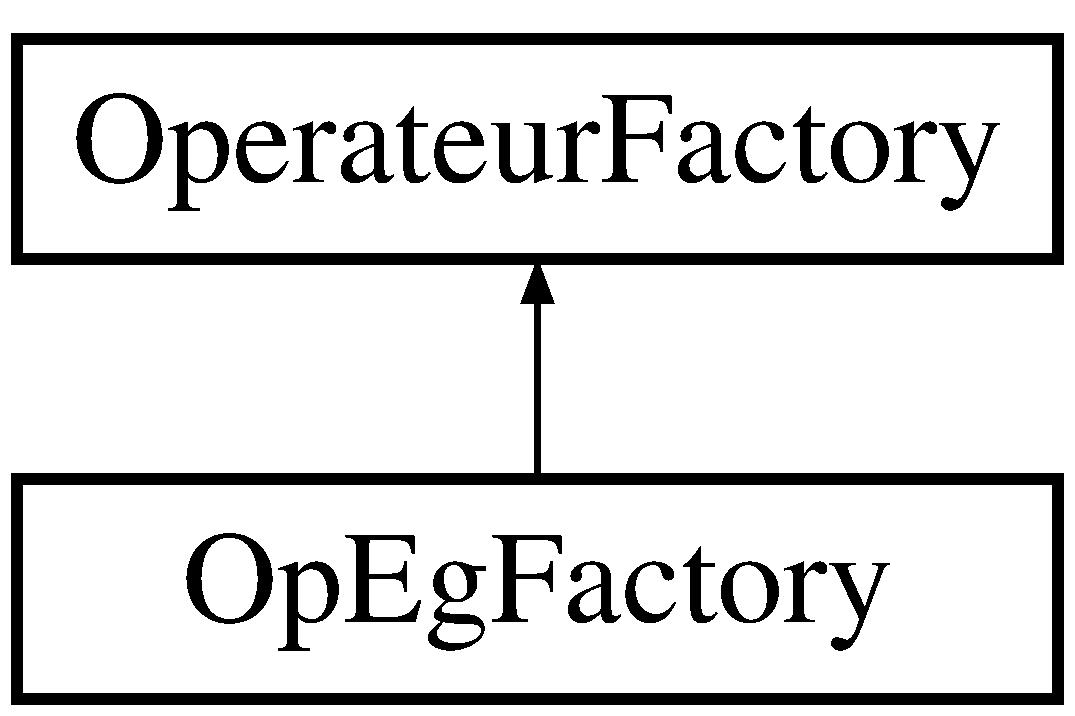
\includegraphics[height=2.000000cm]{class_op_eg_factory}
\end{center}
\end{figure}
\subsection*{Public Member Functions}
\begin{DoxyCompactItemize}
\item 
\hyperlink{class_op_eg_factory_a90175a5618d622d565bce69c690454e1}{Op\+Eg\+Factory} ()
\item 
\hyperlink{class_operateur}{Operateur} $\ast$ \hyperlink{class_op_eg_factory_a672618af98b076339949e129a12d7962}{get\+Operateur} ()
\end{DoxyCompactItemize}
\subsection*{Additional Inherited Members}


\subsection{Detailed Description}


Definition at line 240 of file operator\+Factory.\+h.



\subsection{Constructor \& Destructor Documentation}
\index{Op\+Eg\+Factory@{Op\+Eg\+Factory}!Op\+Eg\+Factory@{Op\+Eg\+Factory}}
\index{Op\+Eg\+Factory@{Op\+Eg\+Factory}!Op\+Eg\+Factory@{Op\+Eg\+Factory}}
\subsubsection[{\texorpdfstring{Op\+Eg\+Factory()}{OpEgFactory()}}]{\setlength{\rightskip}{0pt plus 5cm}Op\+Eg\+Factory\+::\+Op\+Eg\+Factory (
\begin{DoxyParamCaption}
{}
\end{DoxyParamCaption}
)\hspace{0.3cm}{\ttfamily [inline]}}\hypertarget{class_op_eg_factory_a90175a5618d622d565bce69c690454e1}{}\label{class_op_eg_factory_a90175a5618d622d565bce69c690454e1}


Definition at line 242 of file operator\+Factory.\+h.



\subsection{Member Function Documentation}
\index{Op\+Eg\+Factory@{Op\+Eg\+Factory}!get\+Operateur@{get\+Operateur}}
\index{get\+Operateur@{get\+Operateur}!Op\+Eg\+Factory@{Op\+Eg\+Factory}}
\subsubsection[{\texorpdfstring{get\+Operateur()}{getOperateur()}}]{\setlength{\rightskip}{0pt plus 5cm}{\bf Operateur}$\ast$ Op\+Eg\+Factory\+::get\+Operateur (
\begin{DoxyParamCaption}
{}
\end{DoxyParamCaption}
)\hspace{0.3cm}{\ttfamily [inline]}, {\ttfamily [virtual]}}\hypertarget{class_op_eg_factory_a672618af98b076339949e129a12d7962}{}\label{class_op_eg_factory_a672618af98b076339949e129a12d7962}


Implements \hyperlink{class_operateur_factory_aff61b2f67451f086d6abaea4231b2d78}{Operateur\+Factory}.



Definition at line 243 of file operator\+Factory.\+h.



The documentation for this class was generated from the following file\+:\begin{DoxyCompactItemize}
\item 
\hyperlink{operator_factory_8h}{operator\+Factory.\+h}\end{DoxyCompactItemize}

\hypertarget{class_operande}{}\section{Operande Class Reference}
\label{class_operande}\index{Operande@{Operande}}


{\ttfamily \#include $<$litterale.\+h$>$}

Inheritance diagram for Operande\+:\begin{figure}[H]
\begin{center}
\leavevmode
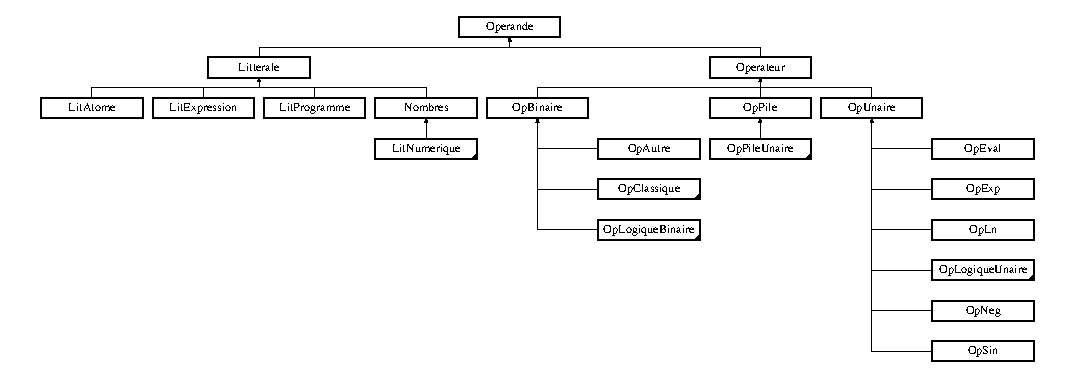
\includegraphics[height=4.628099cm]{class_operande}
\end{center}
\end{figure}
\subsection*{Public Member Functions}
\begin{DoxyCompactItemize}
\item 
\hyperlink{class_operande_acd4af503ef581f5d74f8a2db19fc0e1a}{Operande} (const Q\+String \&na)
\item 
virtual \hyperlink{class_operande_a36c291e8856c7ebcf8278ac5a14575a4}{$\sim$\+Operande} ()
\item 
virtual Q\+String \hyperlink{class_operande_a2acae8f59199e93850b3fdb13eba1672}{to\+String} () const  =0
\item 
Q\+String \& \hyperlink{class_operande_a0b5205c009a81e48a66544bfe819ce30}{get\+Name} ()
\end{DoxyCompactItemize}
\subsection*{Protected Attributes}
\begin{DoxyCompactItemize}
\item 
Q\+String \hyperlink{class_operande_abb638f60898b542d803a146a297706e0}{name}
\end{DoxyCompactItemize}


\subsection{Detailed Description}


Definition at line 18 of file litterale.\+h.



\subsection{Constructor \& Destructor Documentation}
\index{Operande@{Operande}!Operande@{Operande}}
\index{Operande@{Operande}!Operande@{Operande}}
\subsubsection[{\texorpdfstring{Operande(const Q\+String \&na)}{Operande(const QString &na)}}]{\setlength{\rightskip}{0pt plus 5cm}Operande\+::\+Operande (
\begin{DoxyParamCaption}
\item[{const Q\+String \&}]{na}
\end{DoxyParamCaption}
)\hspace{0.3cm}{\ttfamily [inline]}}\hypertarget{class_operande_acd4af503ef581f5d74f8a2db19fc0e1a}{}\label{class_operande_acd4af503ef581f5d74f8a2db19fc0e1a}


Definition at line 22 of file litterale.\+h.

\index{Operande@{Operande}!````~Operande@{$\sim$\+Operande}}
\index{````~Operande@{$\sim$\+Operande}!Operande@{Operande}}
\subsubsection[{\texorpdfstring{$\sim$\+Operande()}{~Operande()}}]{\setlength{\rightskip}{0pt plus 5cm}Operande\+::$\sim$\+Operande (
\begin{DoxyParamCaption}
{}
\end{DoxyParamCaption}
)\hspace{0.3cm}{\ttfamily [virtual]}}\hypertarget{class_operande_a36c291e8856c7ebcf8278ac5a14575a4}{}\label{class_operande_a36c291e8856c7ebcf8278ac5a14575a4}


Definition at line 4 of file litterale.\+cpp.



\subsection{Member Function Documentation}
\index{Operande@{Operande}!get\+Name@{get\+Name}}
\index{get\+Name@{get\+Name}!Operande@{Operande}}
\subsubsection[{\texorpdfstring{get\+Name()}{getName()}}]{\setlength{\rightskip}{0pt plus 5cm}Q\+String\& Operande\+::get\+Name (
\begin{DoxyParamCaption}
{}
\end{DoxyParamCaption}
)\hspace{0.3cm}{\ttfamily [inline]}}\hypertarget{class_operande_a0b5205c009a81e48a66544bfe819ce30}{}\label{class_operande_a0b5205c009a81e48a66544bfe819ce30}


Definition at line 25 of file litterale.\+h.

\index{Operande@{Operande}!to\+String@{to\+String}}
\index{to\+String@{to\+String}!Operande@{Operande}}
\subsubsection[{\texorpdfstring{to\+String() const  =0}{toString() const  =0}}]{\setlength{\rightskip}{0pt plus 5cm}virtual Q\+String Operande\+::to\+String (
\begin{DoxyParamCaption}
{}
\end{DoxyParamCaption}
) const\hspace{0.3cm}{\ttfamily [pure virtual]}}\hypertarget{class_operande_a2acae8f59199e93850b3fdb13eba1672}{}\label{class_operande_a2acae8f59199e93850b3fdb13eba1672}


Implemented in \hyperlink{class_reelle_add2eb8eb352c8bef1e5d51119b54bcb6}{Reelle}, \hyperlink{class_rationnelle_a406d82b3db71b5d7cac720a12e756c3c}{Rationnelle}, \hyperlink{class_entier_aa960356dfeae8af6dfa2cd25136a1a6f}{Entier}, \hyperlink{class_lit_numerique_a6e3c66f0b484c5be954eb788a95c0d16}{Lit\+Numerique}, \hyperlink{class_nombres_a456e2e58403e79cabdfefb14fd19b4f1}{Nombres}, \hyperlink{class_lit_atome_abbe47368e149ae5a9744bc7188df1cc8}{Lit\+Atome}, \hyperlink{class_lit_expression_a108f8809e4ca49343426c9d0c30c28c4}{Lit\+Expression}, \hyperlink{class_lit_programme_a8a1086c6458e02378f66144fe1f841be}{Lit\+Programme}, \hyperlink{class_litterale_a3b427621132af2903259390143d1b16d}{Litterale}, and \hyperlink{class_operateur_ad49ae9c67adcd3af3a9be0e2bc13c629}{Operateur}.



\subsection{Member Data Documentation}
\index{Operande@{Operande}!name@{name}}
\index{name@{name}!Operande@{Operande}}
\subsubsection[{\texorpdfstring{name}{name}}]{\setlength{\rightskip}{0pt plus 5cm}Q\+String Operande\+::name\hspace{0.3cm}{\ttfamily [protected]}}\hypertarget{class_operande_abb638f60898b542d803a146a297706e0}{}\label{class_operande_abb638f60898b542d803a146a297706e0}


Definition at line 20 of file litterale.\+h.



The documentation for this class was generated from the following files\+:\begin{DoxyCompactItemize}
\item 
\hyperlink{litterale_8h}{litterale.\+h}\item 
\hyperlink{litterale_8cpp}{litterale.\+cpp}\end{DoxyCompactItemize}

\hypertarget{class_operateur}{}\section{Operateur Class Reference}
\label{class_operateur}\index{Operateur@{Operateur}}


{\ttfamily \#include $<$operator.\+h$>$}

Inheritance diagram for Operateur\+:\begin{figure}[H]
\begin{center}
\leavevmode
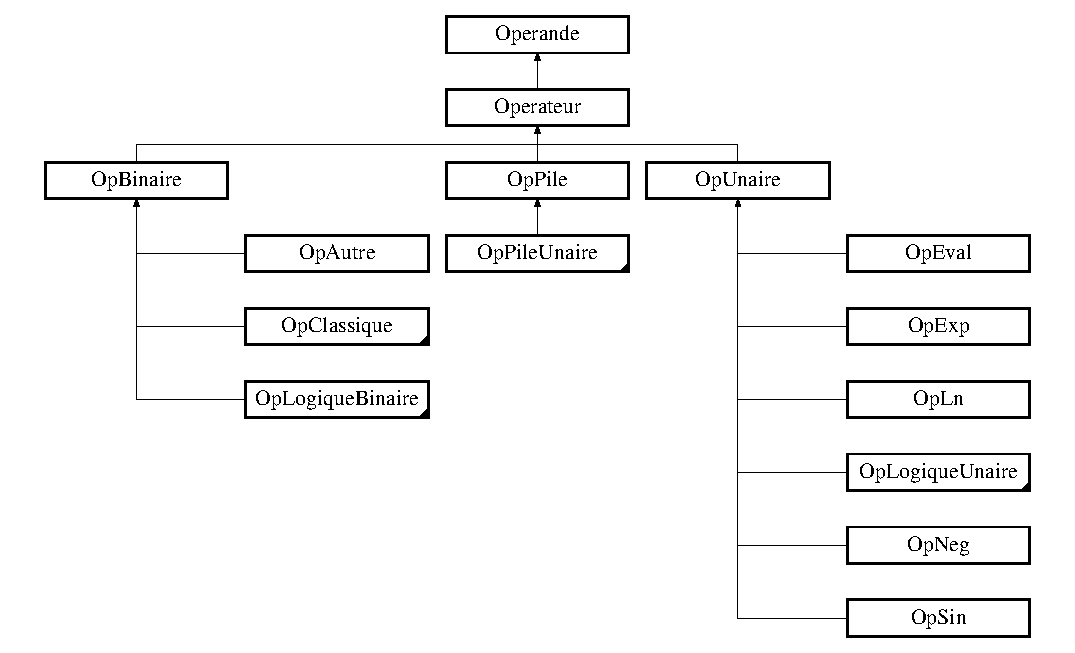
\includegraphics[height=8.330579cm]{class_operateur}
\end{center}
\end{figure}
\subsection*{Public Member Functions}
\begin{DoxyCompactItemize}
\item 
\hyperlink{class_operateur_ad30f42803cab7fbffe07d6b6a3723ee2}{Operateur} (const Q\+String \&na, unsigned int t)
\item 
virtual \hyperlink{class_operateur_a6cf041d43e1cde240783492fc887a54a}{$\sim$\+Operateur} ()
\item 
virtual \hyperlink{class_litterale}{Litterale} $\ast$ \hyperlink{class_operateur_a875ee3c8ad2284fd8537c32070d059d2}{executer} ()=0
\item 
virtual void \hyperlink{class_operateur_ae9b209c3a9f55eb3b3821f43fe437105}{add\+Arg} (\hyperlink{class_pile}{Pile} $\ast$pile)
\item 
virtual void \hyperlink{class_operateur_ae39d95062e174881d250561617cf7a6a}{add\+Arg} (\hyperlink{class_litterale}{Litterale} $\ast$arg1)
\item 
unsigned int \hyperlink{class_operateur_a850af30f5bd589fb9c3f10b9dbc03f73}{get\+Taille} () const 
\item 
Q\+String \hyperlink{class_operateur_ad49ae9c67adcd3af3a9be0e2bc13c629}{to\+String} () const 
\end{DoxyCompactItemize}
\subsection*{Protected Attributes}
\begin{DoxyCompactItemize}
\item 
Q\+Vector$<$ \hyperlink{class_litterale}{Litterale} $\ast$ $>$ \hyperlink{class_operateur_a8f8f737f9d972ac60d1f0d8700cd3857}{tab}
\item 
unsigned int \hyperlink{class_operateur_a616ac1808bc641e898d0ed97f770ffaf}{taille}
\end{DoxyCompactItemize}


\subsection{Detailed Description}


Definition at line 7 of file operator.\+h.



\subsection{Constructor \& Destructor Documentation}
\index{Operateur@{Operateur}!Operateur@{Operateur}}
\index{Operateur@{Operateur}!Operateur@{Operateur}}
\subsubsection[{\texorpdfstring{Operateur(const Q\+String \&na, unsigned int t)}{Operateur(const QString &na, unsigned int t)}}]{\setlength{\rightskip}{0pt plus 5cm}Operateur\+::\+Operateur (
\begin{DoxyParamCaption}
\item[{const Q\+String \&}]{na, }
\item[{unsigned int}]{t}
\end{DoxyParamCaption}
)\hspace{0.3cm}{\ttfamily [inline]}}\hypertarget{class_operateur_ad30f42803cab7fbffe07d6b6a3723ee2}{}\label{class_operateur_ad30f42803cab7fbffe07d6b6a3723ee2}


Definition at line 15 of file operator.\+h.

\index{Operateur@{Operateur}!````~Operateur@{$\sim$\+Operateur}}
\index{````~Operateur@{$\sim$\+Operateur}!Operateur@{Operateur}}
\subsubsection[{\texorpdfstring{$\sim$\+Operateur()}{~Operateur()}}]{\setlength{\rightskip}{0pt plus 5cm}Operateur\+::$\sim$\+Operateur (
\begin{DoxyParamCaption}
{}
\end{DoxyParamCaption}
)\hspace{0.3cm}{\ttfamily [virtual]}}\hypertarget{class_operateur_a6cf041d43e1cde240783492fc887a54a}{}\label{class_operateur_a6cf041d43e1cde240783492fc887a54a}


Definition at line 5 of file operator.\+cpp.



\subsection{Member Function Documentation}
\index{Operateur@{Operateur}!add\+Arg@{add\+Arg}}
\index{add\+Arg@{add\+Arg}!Operateur@{Operateur}}
\subsubsection[{\texorpdfstring{add\+Arg(\+Pile $\ast$pile)}{addArg(Pile *pile)}}]{\setlength{\rightskip}{0pt plus 5cm}void Operateur\+::add\+Arg (
\begin{DoxyParamCaption}
\item[{{\bf Pile} $\ast$}]{pile}
\end{DoxyParamCaption}
)\hspace{0.3cm}{\ttfamily [virtual]}}\hypertarget{class_operateur_ae9b209c3a9f55eb3b3821f43fe437105}{}\label{class_operateur_ae9b209c3a9f55eb3b3821f43fe437105}


Reimplemented in \hyperlink{class_op_pile_ac05c50b3c226d57dbb866442ab8fd5e3}{Op\+Pile}, \hyperlink{class_op_binaire_ac48be97498d47266542ff81c86c1a118}{Op\+Binaire}, and \hyperlink{class_op_unaire_a180e3556bac104e4762b16dc23675afc}{Op\+Unaire}.



Definition at line 11 of file operator.\+cpp.

\index{Operateur@{Operateur}!add\+Arg@{add\+Arg}}
\index{add\+Arg@{add\+Arg}!Operateur@{Operateur}}
\subsubsection[{\texorpdfstring{add\+Arg(\+Litterale $\ast$arg1)}{addArg(Litterale *arg1)}}]{\setlength{\rightskip}{0pt plus 5cm}void Operateur\+::add\+Arg (
\begin{DoxyParamCaption}
\item[{{\bf Litterale} $\ast$}]{arg1}
\end{DoxyParamCaption}
)\hspace{0.3cm}{\ttfamily [virtual]}}\hypertarget{class_operateur_ae39d95062e174881d250561617cf7a6a}{}\label{class_operateur_ae39d95062e174881d250561617cf7a6a}


Reimplemented in \hyperlink{class_op_binaire_af39b73a32c35ed7722fac1d380b92bbd}{Op\+Binaire}, and \hyperlink{class_op_unaire_a7bd766f9358b3d286a29a876ab82ebf6}{Op\+Unaire}.



Definition at line 13 of file operator.\+cpp.

\index{Operateur@{Operateur}!executer@{executer}}
\index{executer@{executer}!Operateur@{Operateur}}
\subsubsection[{\texorpdfstring{executer()=0}{executer()=0}}]{\setlength{\rightskip}{0pt plus 5cm}virtual {\bf Litterale}$\ast$ Operateur\+::executer (
\begin{DoxyParamCaption}
{}
\end{DoxyParamCaption}
)\hspace{0.3cm}{\ttfamily [pure virtual]}}\hypertarget{class_operateur_a875ee3c8ad2284fd8537c32070d059d2}{}\label{class_operateur_a875ee3c8ad2284fd8537c32070d059d2}


Implemented in \hyperlink{class_op_pile_a02b47fa3b5f7399a09681c80353024e0}{Op\+Pile}, \hyperlink{class_op_binaire_aa81570ae3aeb44b9533e7ddd82a397be}{Op\+Binaire}, and \hyperlink{class_op_unaire_a37fd2b7149554eb575280e88e8914ff6}{Op\+Unaire}.

\index{Operateur@{Operateur}!get\+Taille@{get\+Taille}}
\index{get\+Taille@{get\+Taille}!Operateur@{Operateur}}
\subsubsection[{\texorpdfstring{get\+Taille() const }{getTaille() const }}]{\setlength{\rightskip}{0pt plus 5cm}unsigned int Operateur\+::get\+Taille (
\begin{DoxyParamCaption}
{}
\end{DoxyParamCaption}
) const\hspace{0.3cm}{\ttfamily [inline]}}\hypertarget{class_operateur_a850af30f5bd589fb9c3f10b9dbc03f73}{}\label{class_operateur_a850af30f5bd589fb9c3f10b9dbc03f73}


Definition at line 20 of file operator.\+h.

\index{Operateur@{Operateur}!to\+String@{to\+String}}
\index{to\+String@{to\+String}!Operateur@{Operateur}}
\subsubsection[{\texorpdfstring{to\+String() const }{toString() const }}]{\setlength{\rightskip}{0pt plus 5cm}Q\+String Operateur\+::to\+String (
\begin{DoxyParamCaption}
{}
\end{DoxyParamCaption}
) const\hspace{0.3cm}{\ttfamily [inline]}, {\ttfamily [virtual]}}\hypertarget{class_operateur_ad49ae9c67adcd3af3a9be0e2bc13c629}{}\label{class_operateur_ad49ae9c67adcd3af3a9be0e2bc13c629}


Implements \hyperlink{class_operande_a2acae8f59199e93850b3fdb13eba1672}{Operande}.



Definition at line 21 of file operator.\+h.



\subsection{Member Data Documentation}
\index{Operateur@{Operateur}!tab@{tab}}
\index{tab@{tab}!Operateur@{Operateur}}
\subsubsection[{\texorpdfstring{tab}{tab}}]{\setlength{\rightskip}{0pt plus 5cm}Q\+Vector$<${\bf Litterale}$\ast$$>$ Operateur\+::tab\hspace{0.3cm}{\ttfamily [protected]}}\hypertarget{class_operateur_a8f8f737f9d972ac60d1f0d8700cd3857}{}\label{class_operateur_a8f8f737f9d972ac60d1f0d8700cd3857}


Definition at line 11 of file operator.\+h.

\index{Operateur@{Operateur}!taille@{taille}}
\index{taille@{taille}!Operateur@{Operateur}}
\subsubsection[{\texorpdfstring{taille}{taille}}]{\setlength{\rightskip}{0pt plus 5cm}unsigned int Operateur\+::taille\hspace{0.3cm}{\ttfamily [protected]}}\hypertarget{class_operateur_a616ac1808bc641e898d0ed97f770ffaf}{}\label{class_operateur_a616ac1808bc641e898d0ed97f770ffaf}


Definition at line 12 of file operator.\+h.



The documentation for this class was generated from the following files\+:\begin{DoxyCompactItemize}
\item 
\hyperlink{operator_8h}{operator.\+h}\item 
\hyperlink{operator_8cpp}{operator.\+cpp}\end{DoxyCompactItemize}

\hypertarget{class_operateur_factory}{}\section{Operateur\+Factory Class Reference}
\label{class_operateur_factory}\index{Operateur\+Factory@{Operateur\+Factory}}


{\ttfamily \#include $<$operator\+Factory.\+h$>$}

Inheritance diagram for Operateur\+Factory\+:\begin{figure}[H]
\begin{center}
\leavevmode
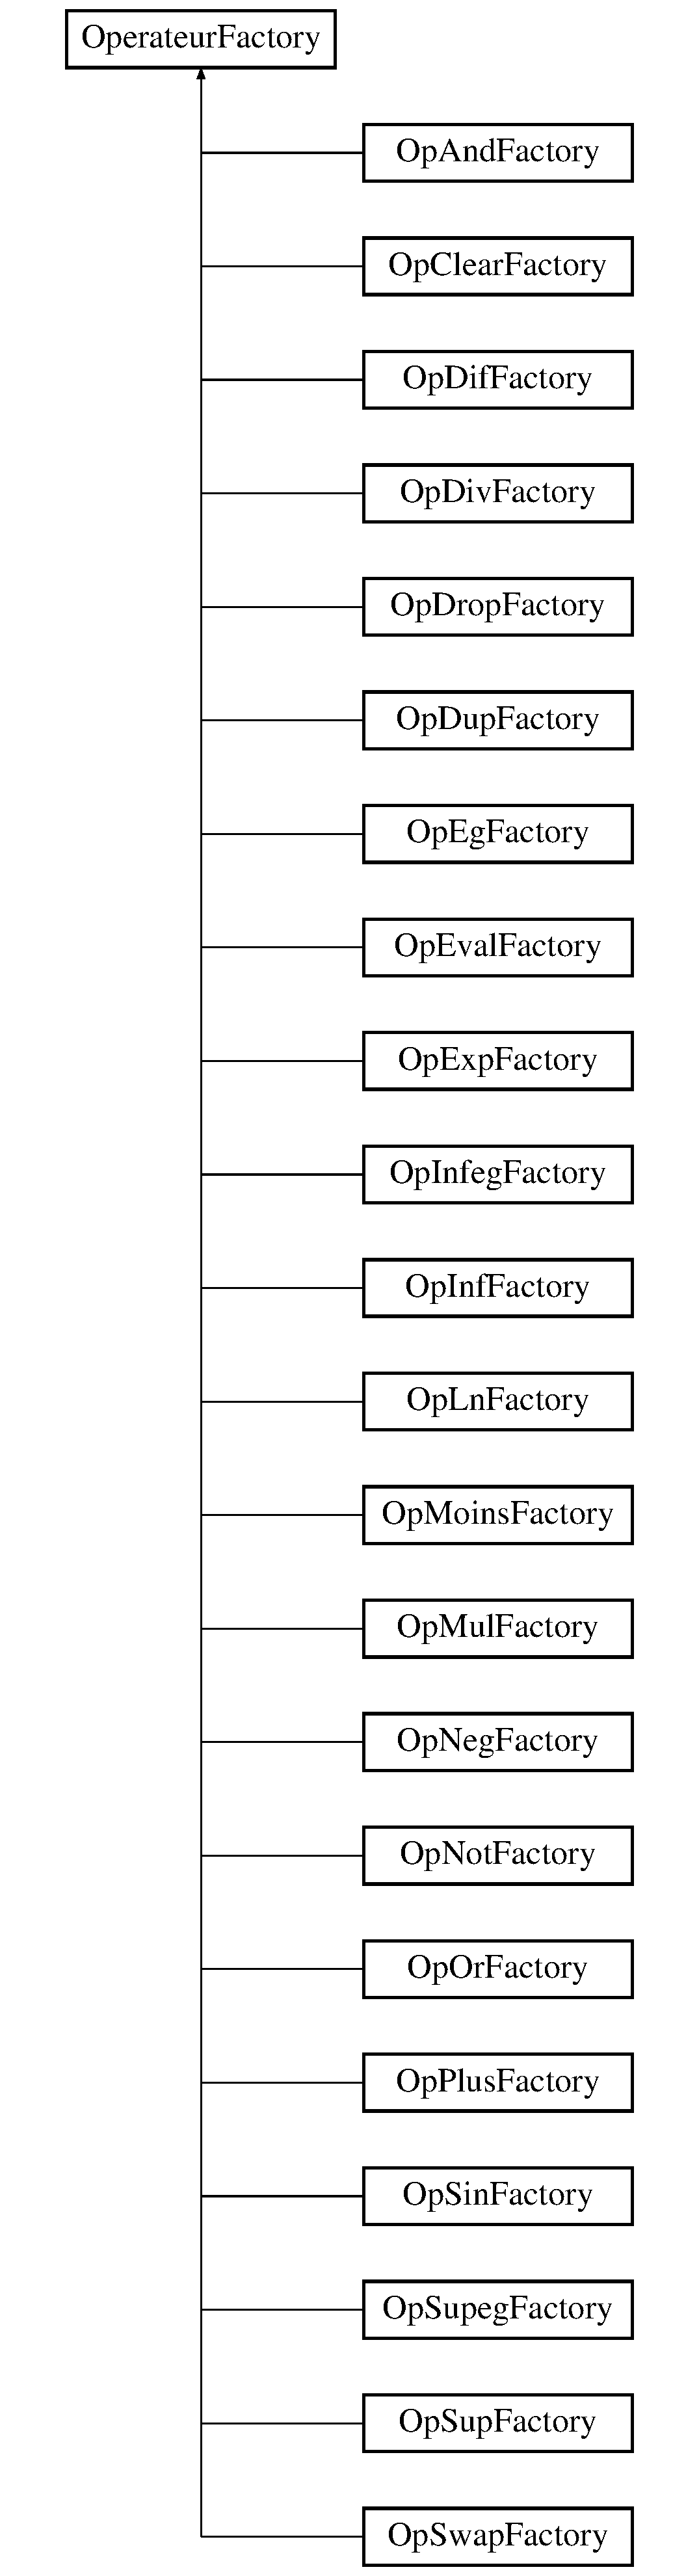
\includegraphics[height=12.000000cm]{class_operateur_factory}
\end{center}
\end{figure}
\subsection*{Public Member Functions}
\begin{DoxyCompactItemize}
\item 
virtual \hyperlink{class_operateur_factory_a2f1c0540a6b9605d1f9ab991c74f92f5}{$\sim$\+Operateur\+Factory} ()
\item 
virtual \hyperlink{class_operateur}{Operateur} $\ast$ \hyperlink{class_operateur_factory_aff61b2f67451f086d6abaea4231b2d78}{get\+Operateur} ()=0
\end{DoxyCompactItemize}
\subsection*{Static Public Member Functions}
\begin{DoxyCompactItemize}
\item 
static Q\+Map$<$ Q\+String, \hyperlink{class_operateur_factory}{Operateur\+Factory} $\ast$ $>$ \hyperlink{class_operateur_factory_a47799a289befae26b8bf162f78bc065c}{get\+Factories\+Map} ()
\end{DoxyCompactItemize}


\subsection{Detailed Description}


Definition at line 14 of file operator\+Factory.\+h.



\subsection{Constructor \& Destructor Documentation}
\index{Operateur\+Factory@{Operateur\+Factory}!````~Operateur\+Factory@{$\sim$\+Operateur\+Factory}}
\index{````~Operateur\+Factory@{$\sim$\+Operateur\+Factory}!Operateur\+Factory@{Operateur\+Factory}}
\subsubsection[{\texorpdfstring{$\sim$\+Operateur\+Factory()}{~OperateurFactory()}}]{\setlength{\rightskip}{0pt plus 5cm}Operateur\+Factory\+::$\sim$\+Operateur\+Factory (
\begin{DoxyParamCaption}
{}
\end{DoxyParamCaption}
)\hspace{0.3cm}{\ttfamily [virtual]}}\hypertarget{class_operateur_factory_a2f1c0540a6b9605d1f9ab991c74f92f5}{}\label{class_operateur_factory_a2f1c0540a6b9605d1f9ab991c74f92f5}


Definition at line 3 of file operator\+Factory.\+cpp.



\subsection{Member Function Documentation}
\index{Operateur\+Factory@{Operateur\+Factory}!get\+Factories\+Map@{get\+Factories\+Map}}
\index{get\+Factories\+Map@{get\+Factories\+Map}!Operateur\+Factory@{Operateur\+Factory}}
\subsubsection[{\texorpdfstring{get\+Factories\+Map()}{getFactoriesMap()}}]{\setlength{\rightskip}{0pt plus 5cm}Q\+Map$<$ Q\+String, {\bf Operateur\+Factory} $\ast$ $>$ Operateur\+Factory\+::get\+Factories\+Map (
\begin{DoxyParamCaption}
{}
\end{DoxyParamCaption}
)\hspace{0.3cm}{\ttfamily [static]}}\hypertarget{class_operateur_factory_a47799a289befae26b8bf162f78bc065c}{}\label{class_operateur_factory_a47799a289befae26b8bf162f78bc065c}


Definition at line 8 of file operator\+Factory.\+cpp.

\index{Operateur\+Factory@{Operateur\+Factory}!get\+Operateur@{get\+Operateur}}
\index{get\+Operateur@{get\+Operateur}!Operateur\+Factory@{Operateur\+Factory}}
\subsubsection[{\texorpdfstring{get\+Operateur()=0}{getOperateur()=0}}]{\setlength{\rightskip}{0pt plus 5cm}virtual {\bf Operateur}$\ast$ Operateur\+Factory\+::get\+Operateur (
\begin{DoxyParamCaption}
{}
\end{DoxyParamCaption}
)\hspace{0.3cm}{\ttfamily [pure virtual]}}\hypertarget{class_operateur_factory_aff61b2f67451f086d6abaea4231b2d78}{}\label{class_operateur_factory_aff61b2f67451f086d6abaea4231b2d78}


Implemented in \hyperlink{class_op_swap_factory_a118491d689bd0d5f28ec1f21b96cbf94}{Op\+Swap\+Factory}, \hyperlink{class_op_dif_factory_af81849fc1a121fa627e7a17e60bed6bc}{Op\+Dif\+Factory}, \hyperlink{class_op_eg_factory_a672618af98b076339949e129a12d7962}{Op\+Eg\+Factory}, \hyperlink{class_op_div_factory_a6bb0a4145ccbafdc3f8016c85bff7be6}{Op\+Div\+Factory}, \hyperlink{class_op_mul_factory_a05fcb523c96c05b6b86d83b56cd49038}{Op\+Mul\+Factory}, \hyperlink{class_op_moins_factory_a4caeb81946c415b7a547871c606c8888}{Op\+Moins\+Factory}, \hyperlink{class_op_plus_factory_aa18f14c6692d7e577a2c3c69ec542066}{Op\+Plus\+Factory}, \hyperlink{class_op_not_factory_a375472ef36be910af8d81983e9237ca7}{Op\+Not\+Factory}, \hyperlink{class_op_or_factory_a6b703fc7860b9ceda4f33c7820081f9b}{Op\+Or\+Factory}, \hyperlink{class_op_and_factory_a7ecd98d30de9c030435385fdeba14566}{Op\+And\+Factory}, \hyperlink{class_op_sup_factory_a6c097723a8510a5b866c56294497becc}{Op\+Sup\+Factory}, \hyperlink{class_op_inf_factory_a981b37a05ef2f71278fa1a91b0e353d8}{Op\+Inf\+Factory}, \hyperlink{class_op_supeg_factory_a0d8201361127228c07343f397ef02134}{Op\+Supeg\+Factory}, \hyperlink{class_op_infeg_factory_a3acf85e418fa861d09ca3272ae643ed5}{Op\+Infeg\+Factory}, \hyperlink{class_op_clear_factory_abd8485d0461c7ae160bebbb3c7f18622}{Op\+Clear\+Factory}, \hyperlink{class_op_drop_factory_af8741d23a6de569d9997adcfb9410efb}{Op\+Drop\+Factory}, \hyperlink{class_op_dup_factory_a5e10a3addcdcfd660c13458408e78359}{Op\+Dup\+Factory}, \hyperlink{class_op_sin_factory_aa252973352a4079b0fc89d17488075a9}{Op\+Sin\+Factory}, \hyperlink{class_op_neg_factory_a7f6cc922bb250ba8da46bfb26bd4acdc}{Op\+Neg\+Factory}, \hyperlink{class_op_eval_factory_a474397933ca39498908039ef40227f55}{Op\+Eval\+Factory}, \hyperlink{class_op_ln_factory_a9634e94728f2ea42f08cc84b40e36629}{Op\+Ln\+Factory}, and \hyperlink{class_op_exp_factory_aafd85b36d415dcb8d7931d6f2a2bf826}{Op\+Exp\+Factory}.



The documentation for this class was generated from the following files\+:\begin{DoxyCompactItemize}
\item 
\hyperlink{operator_factory_8h}{operator\+Factory.\+h}\item 
\hyperlink{operator_factory_8cpp}{operator\+Factory.\+cpp}\end{DoxyCompactItemize}

\hypertarget{class_op_eval}{}\section{Op\+Eval Class Reference}
\label{class_op_eval}\index{Op\+Eval@{Op\+Eval}}


{\ttfamily \#include $<$operator.\+h$>$}

Inheritance diagram for Op\+Eval\+:\begin{figure}[H]
\begin{center}
\leavevmode
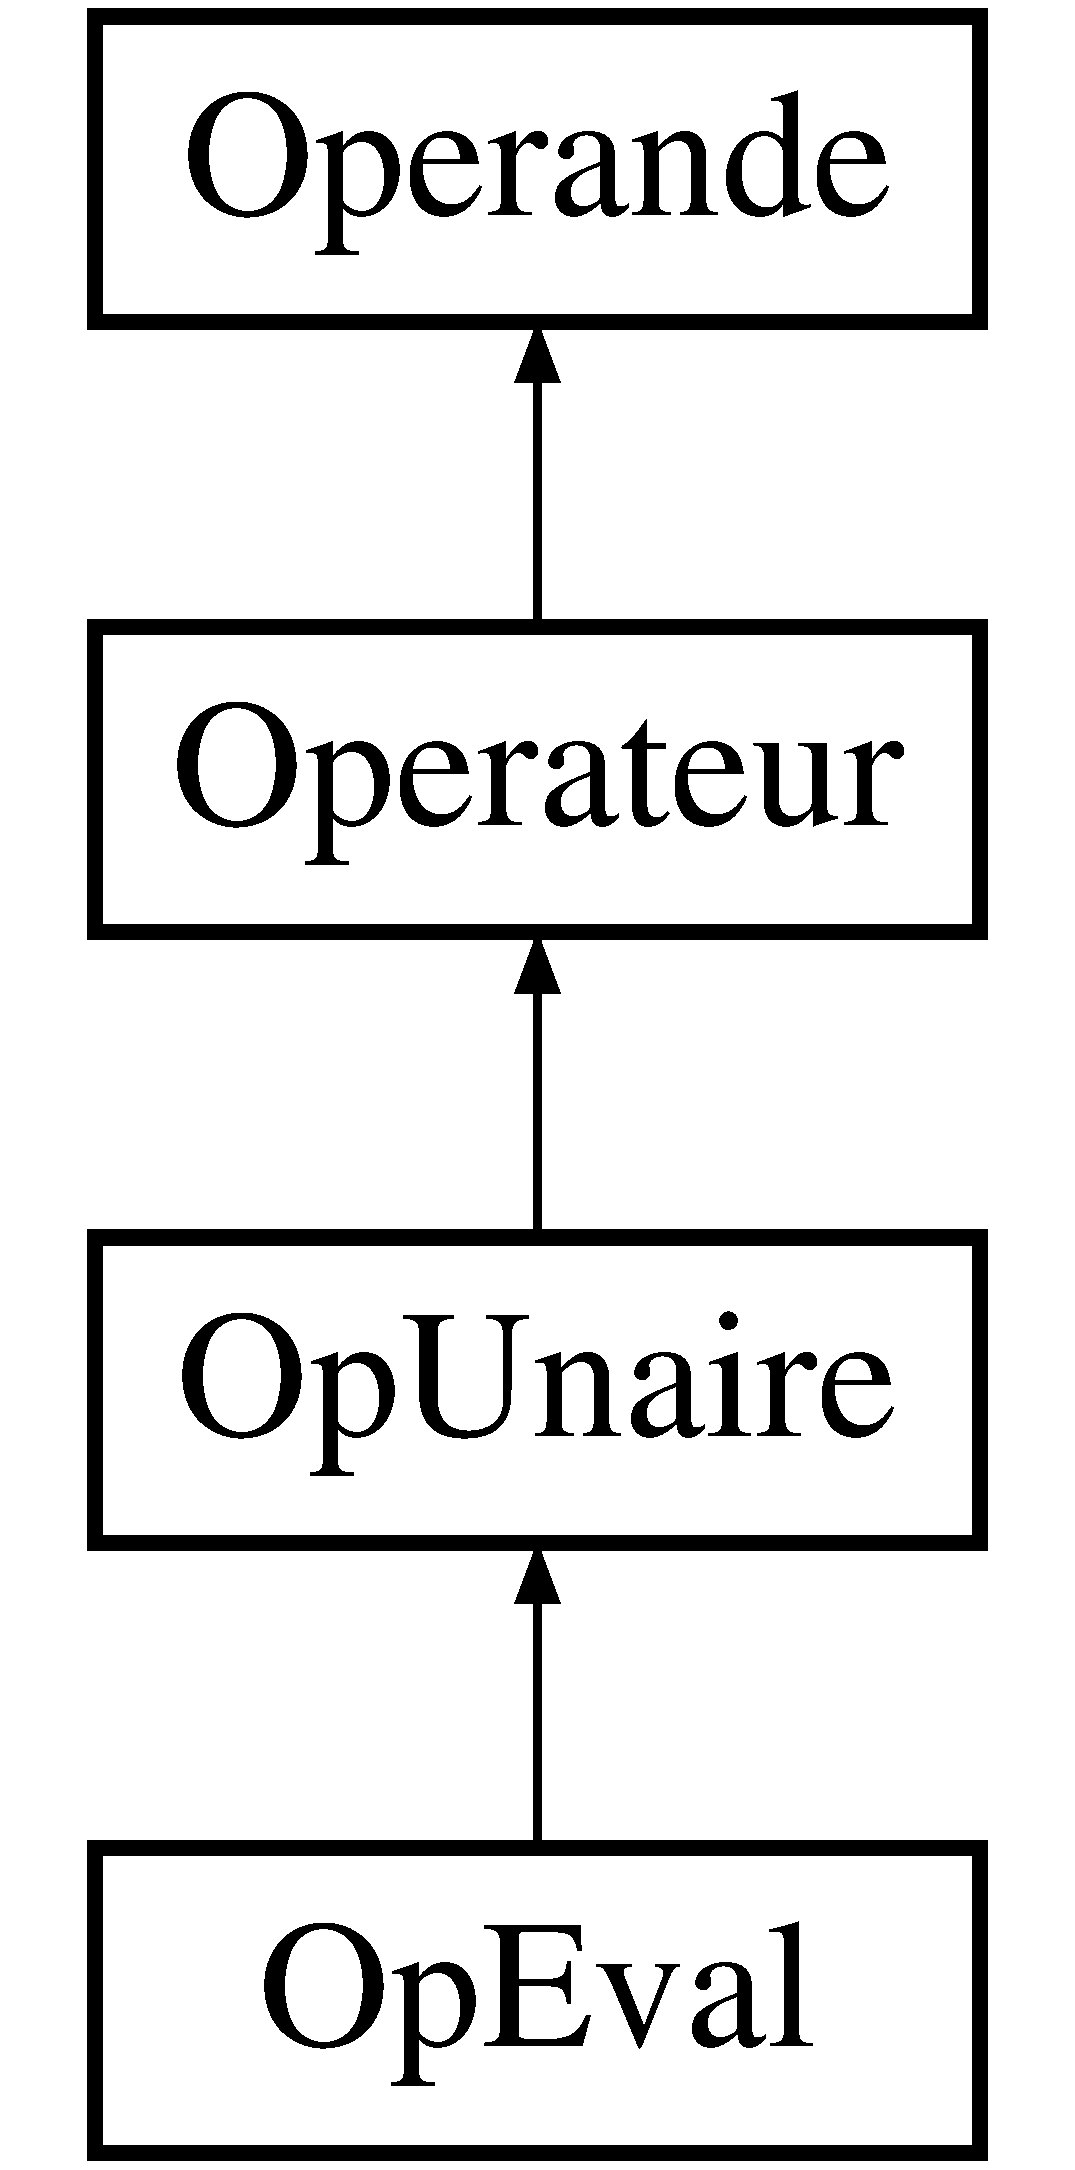
\includegraphics[height=4.000000cm]{class_op_eval}
\end{center}
\end{figure}
\subsection*{Public Member Functions}
\begin{DoxyCompactItemize}
\item 
\hyperlink{class_op_eval_a936d2baca811dbe01a8a4fb3e40176cc}{Op\+Eval} ()
\item 
\hyperlink{class_litterale}{Litterale} $\ast$ \hyperlink{class_op_eval_a1b949d04bab4f73df520319fa70befc9}{fonction\+Expression} (\hyperlink{class_lit_expression}{Lit\+Expression} $\ast$arg1)
\item 
\hyperlink{class_litterale}{Litterale} $\ast$ \hyperlink{class_op_eval_a08658b2923120466790285bc4100783b}{Evaluation} (Q\+Vector$<$ \hyperlink{class_operande}{Operande} $\ast$ $>$ \&vec)
\item 
\hyperlink{class_litterale}{Litterale} $\ast$ \hyperlink{class_op_eval_a4b18ba29a4c6dbc0ce5209649be31135}{action\+Num} (\hyperlink{class_entier}{Entier} \&arg1)
\item 
\hyperlink{class_litterale}{Litterale} $\ast$ \hyperlink{class_op_eval_a56b918642321c739817131a3623a9a9b}{action\+Num} (\hyperlink{class_reelle}{Reelle} \&arg1)
\item 
\hyperlink{class_litterale}{Litterale} $\ast$ \hyperlink{class_op_eval_a793878476d51abf60bed8e78206394b1}{action\+Num} (\hyperlink{class_rationnelle}{Rationnelle} \&arg1)
\end{DoxyCompactItemize}
\subsection*{Additional Inherited Members}


\subsection{Detailed Description}


Definition at line 116 of file operator.\+h.



\subsection{Constructor \& Destructor Documentation}
\index{Op\+Eval@{Op\+Eval}!Op\+Eval@{Op\+Eval}}
\index{Op\+Eval@{Op\+Eval}!Op\+Eval@{Op\+Eval}}
\subsubsection[{\texorpdfstring{Op\+Eval()}{OpEval()}}]{\setlength{\rightskip}{0pt plus 5cm}Op\+Eval\+::\+Op\+Eval (
\begin{DoxyParamCaption}
{}
\end{DoxyParamCaption}
)\hspace{0.3cm}{\ttfamily [inline]}}\hypertarget{class_op_eval_a936d2baca811dbe01a8a4fb3e40176cc}{}\label{class_op_eval_a936d2baca811dbe01a8a4fb3e40176cc}


Definition at line 118 of file operator.\+h.



\subsection{Member Function Documentation}
\index{Op\+Eval@{Op\+Eval}!action\+Num@{action\+Num}}
\index{action\+Num@{action\+Num}!Op\+Eval@{Op\+Eval}}
\subsubsection[{\texorpdfstring{action\+Num(\+Entier \&arg1)}{actionNum(Entier &arg1)}}]{\setlength{\rightskip}{0pt plus 5cm}{\bf Litterale} $\ast$ Op\+Eval\+::action\+Num (
\begin{DoxyParamCaption}
\item[{{\bf Entier} \&}]{arg1}
\end{DoxyParamCaption}
)\hspace{0.3cm}{\ttfamily [virtual]}}\hypertarget{class_op_eval_a4b18ba29a4c6dbc0ce5209649be31135}{}\label{class_op_eval_a4b18ba29a4c6dbc0ce5209649be31135}


Implements \hyperlink{class_op_unaire_a4db1c0cbd6ec4acbe89a6ef2ae68f901}{Op\+Unaire}.



Definition at line 109 of file operator.\+cpp.

\index{Op\+Eval@{Op\+Eval}!action\+Num@{action\+Num}}
\index{action\+Num@{action\+Num}!Op\+Eval@{Op\+Eval}}
\subsubsection[{\texorpdfstring{action\+Num(\+Reelle \&arg1)}{actionNum(Reelle &arg1)}}]{\setlength{\rightskip}{0pt plus 5cm}{\bf Litterale} $\ast$ Op\+Eval\+::action\+Num (
\begin{DoxyParamCaption}
\item[{{\bf Reelle} \&}]{arg1}
\end{DoxyParamCaption}
)\hspace{0.3cm}{\ttfamily [virtual]}}\hypertarget{class_op_eval_a56b918642321c739817131a3623a9a9b}{}\label{class_op_eval_a56b918642321c739817131a3623a9a9b}


Implements \hyperlink{class_op_unaire_a0b92d632cf248e765783f23d6d637d1f}{Op\+Unaire}.



Definition at line 112 of file operator.\+cpp.

\index{Op\+Eval@{Op\+Eval}!action\+Num@{action\+Num}}
\index{action\+Num@{action\+Num}!Op\+Eval@{Op\+Eval}}
\subsubsection[{\texorpdfstring{action\+Num(\+Rationnelle \&arg1)}{actionNum(Rationnelle &arg1)}}]{\setlength{\rightskip}{0pt plus 5cm}{\bf Litterale} $\ast$ Op\+Eval\+::action\+Num (
\begin{DoxyParamCaption}
\item[{{\bf Rationnelle} \&}]{arg1}
\end{DoxyParamCaption}
)\hspace{0.3cm}{\ttfamily [virtual]}}\hypertarget{class_op_eval_a793878476d51abf60bed8e78206394b1}{}\label{class_op_eval_a793878476d51abf60bed8e78206394b1}


Implements \hyperlink{class_op_unaire_a7728e3d41bfe8ace1f9343a4cd404502}{Op\+Unaire}.



Definition at line 115 of file operator.\+cpp.

\index{Op\+Eval@{Op\+Eval}!Evaluation@{Evaluation}}
\index{Evaluation@{Evaluation}!Op\+Eval@{Op\+Eval}}
\subsubsection[{\texorpdfstring{Evaluation(\+Q\+Vector$<$ Operande $\ast$ $>$ \&vec)}{Evaluation(QVector< Operande * > &vec)}}]{\setlength{\rightskip}{0pt plus 5cm}{\bf Litterale} $\ast$ Op\+Eval\+::\+Evaluation (
\begin{DoxyParamCaption}
\item[{Q\+Vector$<$ {\bf Operande} $\ast$ $>$ \&}]{vec}
\end{DoxyParamCaption}
)}\hypertarget{class_op_eval_a08658b2923120466790285bc4100783b}{}\label{class_op_eval_a08658b2923120466790285bc4100783b}


Definition at line 95 of file operator.\+cpp.

\index{Op\+Eval@{Op\+Eval}!fonction\+Expression@{fonction\+Expression}}
\index{fonction\+Expression@{fonction\+Expression}!Op\+Eval@{Op\+Eval}}
\subsubsection[{\texorpdfstring{fonction\+Expression(\+Lit\+Expression $\ast$arg1)}{fonctionExpression(LitExpression *arg1)}}]{\setlength{\rightskip}{0pt plus 5cm}{\bf Litterale} $\ast$ Op\+Eval\+::fonction\+Expression (
\begin{DoxyParamCaption}
\item[{{\bf Lit\+Expression} $\ast$}]{arg1}
\end{DoxyParamCaption}
)\hspace{0.3cm}{\ttfamily [virtual]}}\hypertarget{class_op_eval_a1b949d04bab4f73df520319fa70befc9}{}\label{class_op_eval_a1b949d04bab4f73df520319fa70befc9}


Reimplemented from \hyperlink{class_op_unaire_aba2ca8e42f0fb230de466114eab02f62}{Op\+Unaire}.



Definition at line 85 of file operator.\+cpp.



The documentation for this class was generated from the following files\+:\begin{DoxyCompactItemize}
\item 
\hyperlink{operator_8h}{operator.\+h}\item 
\hyperlink{operator_8cpp}{operator.\+cpp}\end{DoxyCompactItemize}

\hypertarget{class_op_eval_factory}{}\section{Op\+Eval\+Factory Class Reference}
\label{class_op_eval_factory}\index{Op\+Eval\+Factory@{Op\+Eval\+Factory}}


{\ttfamily \#include $<$operator\+Factory.\+h$>$}

Inheritance diagram for Op\+Eval\+Factory\+:\begin{figure}[H]
\begin{center}
\leavevmode
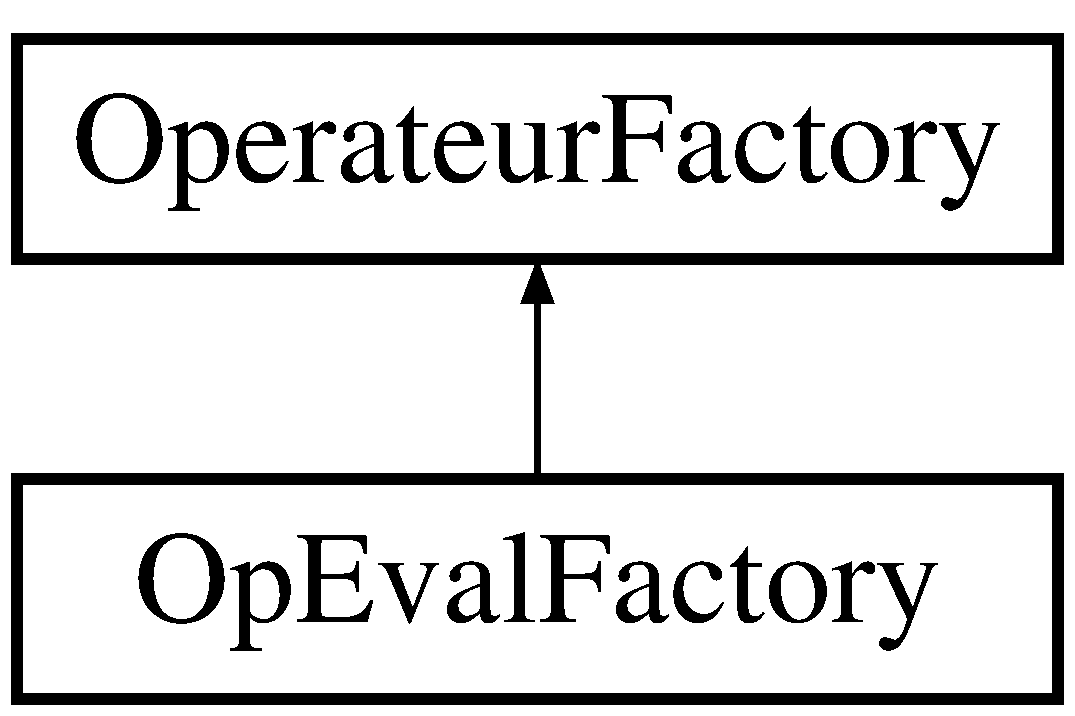
\includegraphics[height=2.000000cm]{class_op_eval_factory}
\end{center}
\end{figure}
\subsection*{Public Member Functions}
\begin{DoxyCompactItemize}
\item 
\hyperlink{class_op_eval_factory_acae8f9988ca1075c848a30a1cbb46da0}{Op\+Eval\+Factory} ()
\item 
\hyperlink{class_operateur}{Operateur} $\ast$ \hyperlink{class_op_eval_factory_a474397933ca39498908039ef40227f55}{get\+Operateur} ()
\end{DoxyCompactItemize}
\subsection*{Additional Inherited Members}


\subsection{Detailed Description}


Definition at line 69 of file operator\+Factory.\+h.



\subsection{Constructor \& Destructor Documentation}
\index{Op\+Eval\+Factory@{Op\+Eval\+Factory}!Op\+Eval\+Factory@{Op\+Eval\+Factory}}
\index{Op\+Eval\+Factory@{Op\+Eval\+Factory}!Op\+Eval\+Factory@{Op\+Eval\+Factory}}
\subsubsection[{\texorpdfstring{Op\+Eval\+Factory()}{OpEvalFactory()}}]{\setlength{\rightskip}{0pt plus 5cm}Op\+Eval\+Factory\+::\+Op\+Eval\+Factory (
\begin{DoxyParamCaption}
{}
\end{DoxyParamCaption}
)\hspace{0.3cm}{\ttfamily [inline]}}\hypertarget{class_op_eval_factory_acae8f9988ca1075c848a30a1cbb46da0}{}\label{class_op_eval_factory_acae8f9988ca1075c848a30a1cbb46da0}


Definition at line 71 of file operator\+Factory.\+h.



\subsection{Member Function Documentation}
\index{Op\+Eval\+Factory@{Op\+Eval\+Factory}!get\+Operateur@{get\+Operateur}}
\index{get\+Operateur@{get\+Operateur}!Op\+Eval\+Factory@{Op\+Eval\+Factory}}
\subsubsection[{\texorpdfstring{get\+Operateur()}{getOperateur()}}]{\setlength{\rightskip}{0pt plus 5cm}{\bf Operateur}$\ast$ Op\+Eval\+Factory\+::get\+Operateur (
\begin{DoxyParamCaption}
{}
\end{DoxyParamCaption}
)\hspace{0.3cm}{\ttfamily [inline]}, {\ttfamily [virtual]}}\hypertarget{class_op_eval_factory_a474397933ca39498908039ef40227f55}{}\label{class_op_eval_factory_a474397933ca39498908039ef40227f55}


Implements \hyperlink{class_operateur_factory_aff61b2f67451f086d6abaea4231b2d78}{Operateur\+Factory}.



Definition at line 72 of file operator\+Factory.\+h.



The documentation for this class was generated from the following file\+:\begin{DoxyCompactItemize}
\item 
\hyperlink{operator_factory_8h}{operator\+Factory.\+h}\end{DoxyCompactItemize}

\hypertarget{class_op_exp}{}\section{Op\+Exp Class Reference}
\label{class_op_exp}\index{Op\+Exp@{Op\+Exp}}


{\ttfamily \#include $<$operator.\+h$>$}

Inheritance diagram for Op\+Exp\+:\begin{figure}[H]
\begin{center}
\leavevmode
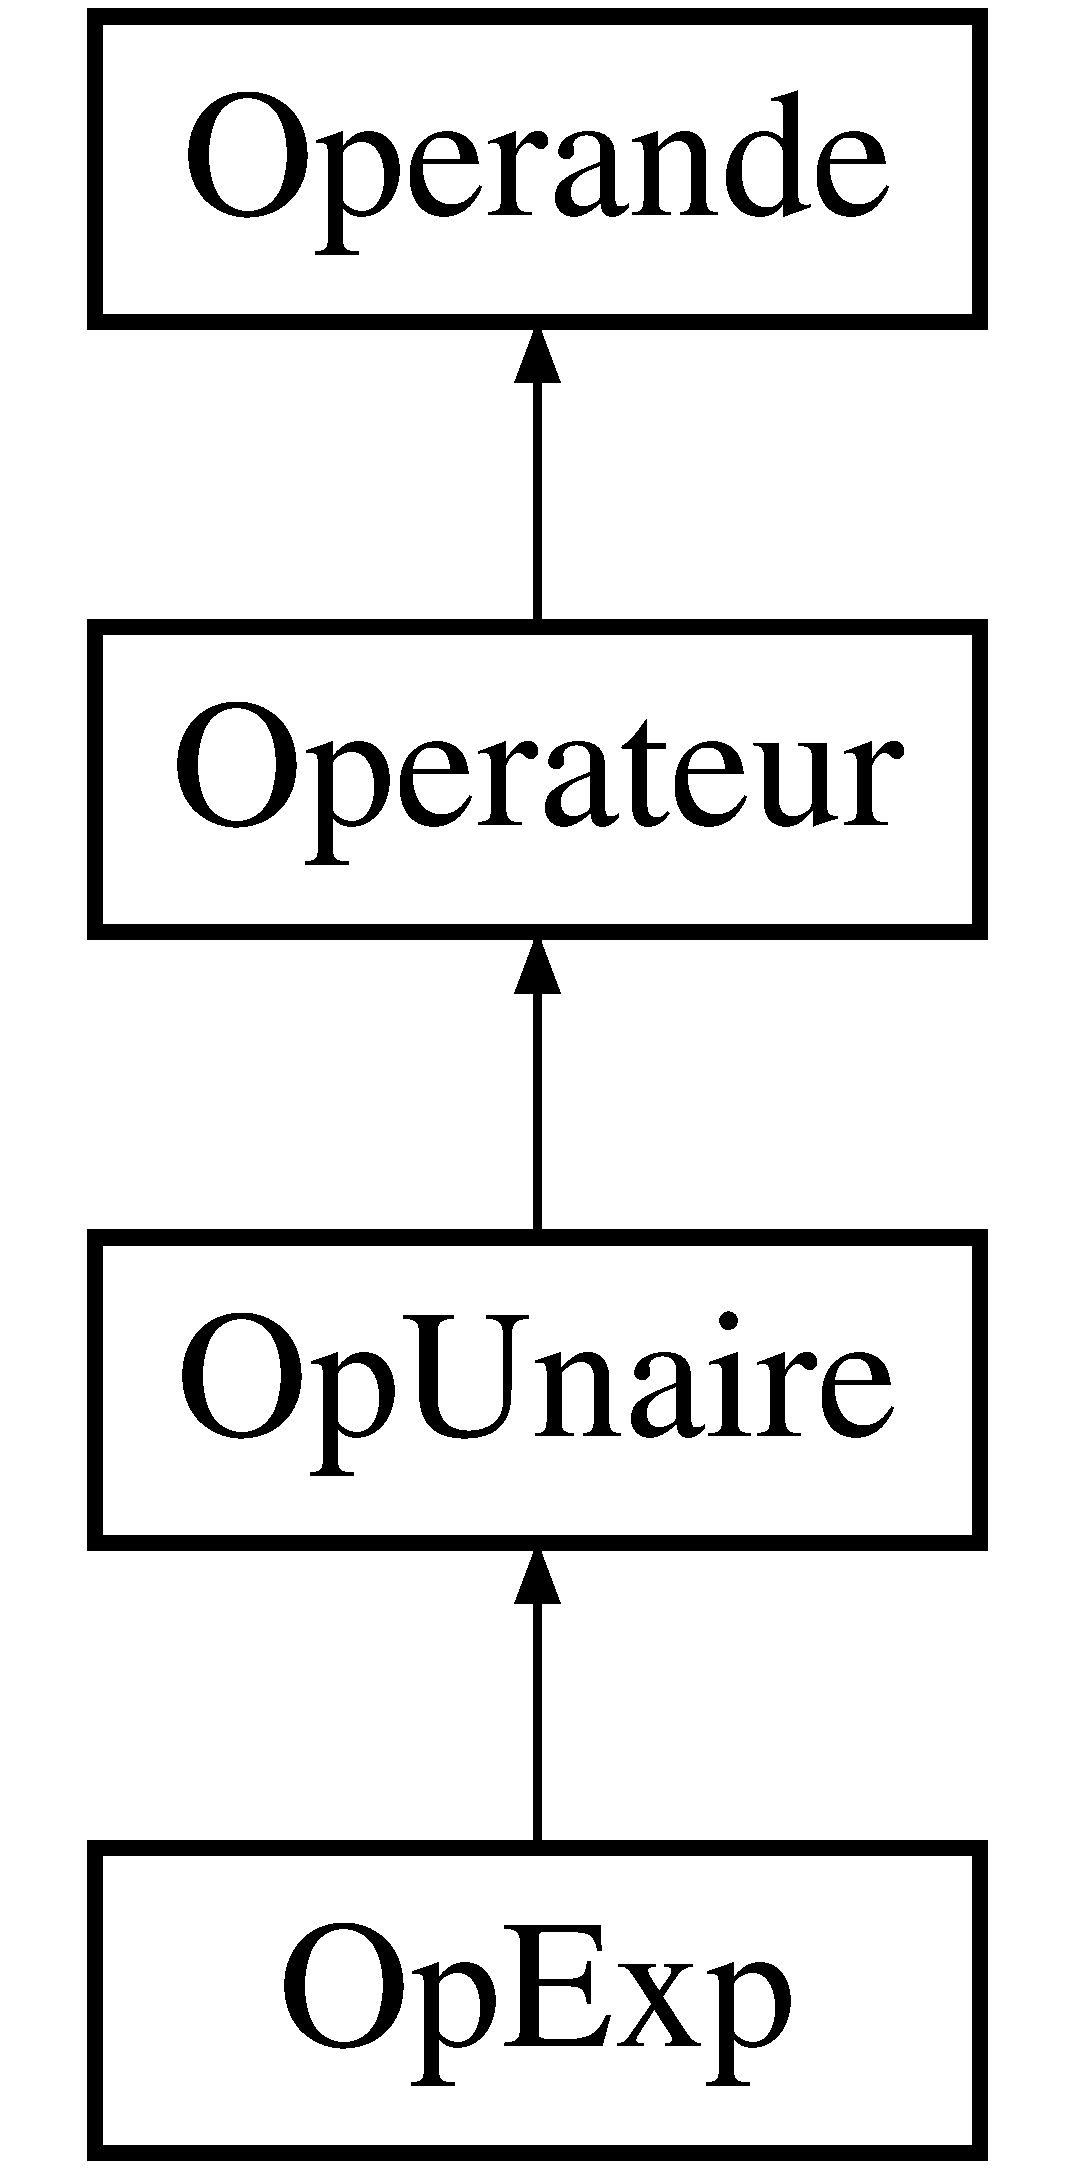
\includegraphics[height=4.000000cm]{class_op_exp}
\end{center}
\end{figure}
\subsection*{Public Member Functions}
\begin{DoxyCompactItemize}
\item 
\hyperlink{class_op_exp_a3b16f95195fab7d0989a9b085759b81e}{Op\+Exp} ()
\item 
\hyperlink{class_litterale}{Litterale} $\ast$ \hyperlink{class_op_exp_a2a7a7e5e698b864749b50b2e33b367fb}{action\+Num} (\hyperlink{class_entier}{Entier} \&arg1)
\item 
\hyperlink{class_litterale}{Litterale} $\ast$ \hyperlink{class_op_exp_ad4ea20ea7b9f02c76eb3a6bdb4455161}{action\+Num} (\hyperlink{class_reelle}{Reelle} \&arg1)
\item 
\hyperlink{class_litterale}{Litterale} $\ast$ \hyperlink{class_op_exp_a1d9e0f1afadd3eeab315b930f250b62e}{action\+Num} (\hyperlink{class_rationnelle}{Rationnelle} \&arg1)
\end{DoxyCompactItemize}
\subsection*{Additional Inherited Members}


\subsection{Detailed Description}


Definition at line 64 of file operator.\+h.



\subsection{Constructor \& Destructor Documentation}
\index{Op\+Exp@{Op\+Exp}!Op\+Exp@{Op\+Exp}}
\index{Op\+Exp@{Op\+Exp}!Op\+Exp@{Op\+Exp}}
\subsubsection[{\texorpdfstring{Op\+Exp()}{OpExp()}}]{\setlength{\rightskip}{0pt plus 5cm}Op\+Exp\+::\+Op\+Exp (
\begin{DoxyParamCaption}
{}
\end{DoxyParamCaption}
)\hspace{0.3cm}{\ttfamily [inline]}}\hypertarget{class_op_exp_a3b16f95195fab7d0989a9b085759b81e}{}\label{class_op_exp_a3b16f95195fab7d0989a9b085759b81e}


Definition at line 66 of file operator.\+h.



\subsection{Member Function Documentation}
\index{Op\+Exp@{Op\+Exp}!action\+Num@{action\+Num}}
\index{action\+Num@{action\+Num}!Op\+Exp@{Op\+Exp}}
\subsubsection[{\texorpdfstring{action\+Num(\+Entier \&arg1)}{actionNum(Entier &arg1)}}]{\setlength{\rightskip}{0pt plus 5cm}{\bf Litterale} $\ast$ Op\+Exp\+::action\+Num (
\begin{DoxyParamCaption}
\item[{{\bf Entier} \&}]{arg1}
\end{DoxyParamCaption}
)\hspace{0.3cm}{\ttfamily [virtual]}}\hypertarget{class_op_exp_a2a7a7e5e698b864749b50b2e33b367fb}{}\label{class_op_exp_a2a7a7e5e698b864749b50b2e33b367fb}


Implements \hyperlink{class_op_unaire_a4db1c0cbd6ec4acbe89a6ef2ae68f901}{Op\+Unaire}.



Definition at line 120 of file operator.\+cpp.

\index{Op\+Exp@{Op\+Exp}!action\+Num@{action\+Num}}
\index{action\+Num@{action\+Num}!Op\+Exp@{Op\+Exp}}
\subsubsection[{\texorpdfstring{action\+Num(\+Reelle \&arg1)}{actionNum(Reelle &arg1)}}]{\setlength{\rightskip}{0pt plus 5cm}{\bf Litterale} $\ast$ Op\+Exp\+::action\+Num (
\begin{DoxyParamCaption}
\item[{{\bf Reelle} \&}]{arg1}
\end{DoxyParamCaption}
)\hspace{0.3cm}{\ttfamily [virtual]}}\hypertarget{class_op_exp_ad4ea20ea7b9f02c76eb3a6bdb4455161}{}\label{class_op_exp_ad4ea20ea7b9f02c76eb3a6bdb4455161}


Implements \hyperlink{class_op_unaire_a0b92d632cf248e765783f23d6d637d1f}{Op\+Unaire}.



Definition at line 124 of file operator.\+cpp.

\index{Op\+Exp@{Op\+Exp}!action\+Num@{action\+Num}}
\index{action\+Num@{action\+Num}!Op\+Exp@{Op\+Exp}}
\subsubsection[{\texorpdfstring{action\+Num(\+Rationnelle \&arg1)}{actionNum(Rationnelle &arg1)}}]{\setlength{\rightskip}{0pt plus 5cm}{\bf Litterale} $\ast$ Op\+Exp\+::action\+Num (
\begin{DoxyParamCaption}
\item[{{\bf Rationnelle} \&}]{arg1}
\end{DoxyParamCaption}
)\hspace{0.3cm}{\ttfamily [virtual]}}\hypertarget{class_op_exp_a1d9e0f1afadd3eeab315b930f250b62e}{}\label{class_op_exp_a1d9e0f1afadd3eeab315b930f250b62e}


Implements \hyperlink{class_op_unaire_a7728e3d41bfe8ace1f9343a4cd404502}{Op\+Unaire}.



Definition at line 129 of file operator.\+cpp.



The documentation for this class was generated from the following files\+:\begin{DoxyCompactItemize}
\item 
\hyperlink{operator_8h}{operator.\+h}\item 
\hyperlink{operator_8cpp}{operator.\+cpp}\end{DoxyCompactItemize}

\hypertarget{class_op_exp_factory}{}\section{Op\+Exp\+Factory Class Reference}
\label{class_op_exp_factory}\index{Op\+Exp\+Factory@{Op\+Exp\+Factory}}


{\ttfamily \#include $<$operator\+Factory.\+h$>$}

Inheritance diagram for Op\+Exp\+Factory\+:\begin{figure}[H]
\begin{center}
\leavevmode
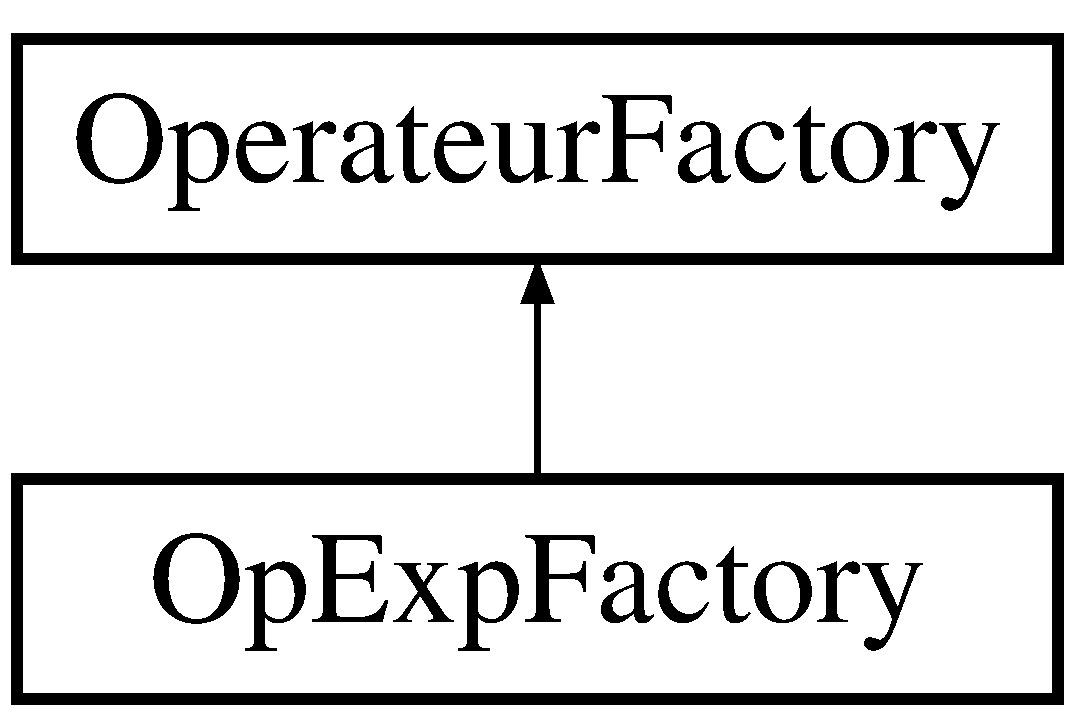
\includegraphics[height=2.000000cm]{class_op_exp_factory}
\end{center}
\end{figure}
\subsection*{Public Member Functions}
\begin{DoxyCompactItemize}
\item 
\hyperlink{class_op_exp_factory_aaebf373dfbe1b1360b43c452aadf76e3}{Op\+Exp\+Factory} ()
\item 
\hyperlink{class_operateur}{Operateur} $\ast$ \hyperlink{class_op_exp_factory_aafd85b36d415dcb8d7931d6f2a2bf826}{get\+Operateur} ()
\end{DoxyCompactItemize}
\subsection*{Additional Inherited Members}


\subsection{Detailed Description}


Definition at line 21 of file operator\+Factory.\+h.



\subsection{Constructor \& Destructor Documentation}
\index{Op\+Exp\+Factory@{Op\+Exp\+Factory}!Op\+Exp\+Factory@{Op\+Exp\+Factory}}
\index{Op\+Exp\+Factory@{Op\+Exp\+Factory}!Op\+Exp\+Factory@{Op\+Exp\+Factory}}
\subsubsection[{\texorpdfstring{Op\+Exp\+Factory()}{OpExpFactory()}}]{\setlength{\rightskip}{0pt plus 5cm}Op\+Exp\+Factory\+::\+Op\+Exp\+Factory (
\begin{DoxyParamCaption}
{}
\end{DoxyParamCaption}
)\hspace{0.3cm}{\ttfamily [inline]}}\hypertarget{class_op_exp_factory_aaebf373dfbe1b1360b43c452aadf76e3}{}\label{class_op_exp_factory_aaebf373dfbe1b1360b43c452aadf76e3}


Definition at line 23 of file operator\+Factory.\+h.



\subsection{Member Function Documentation}
\index{Op\+Exp\+Factory@{Op\+Exp\+Factory}!get\+Operateur@{get\+Operateur}}
\index{get\+Operateur@{get\+Operateur}!Op\+Exp\+Factory@{Op\+Exp\+Factory}}
\subsubsection[{\texorpdfstring{get\+Operateur()}{getOperateur()}}]{\setlength{\rightskip}{0pt plus 5cm}{\bf Operateur}$\ast$ Op\+Exp\+Factory\+::get\+Operateur (
\begin{DoxyParamCaption}
{}
\end{DoxyParamCaption}
)\hspace{0.3cm}{\ttfamily [inline]}, {\ttfamily [virtual]}}\hypertarget{class_op_exp_factory_aafd85b36d415dcb8d7931d6f2a2bf826}{}\label{class_op_exp_factory_aafd85b36d415dcb8d7931d6f2a2bf826}


Implements \hyperlink{class_operateur_factory_aff61b2f67451f086d6abaea4231b2d78}{Operateur\+Factory}.



Definition at line 24 of file operator\+Factory.\+h.



The documentation for this class was generated from the following file\+:\begin{DoxyCompactItemize}
\item 
\hyperlink{operator_factory_8h}{operator\+Factory.\+h}\end{DoxyCompactItemize}

\hypertarget{class_op_inf}{}\section{Op\+Inf Class Reference}
\label{class_op_inf}\index{Op\+Inf@{Op\+Inf}}


{\ttfamily \#include $<$operator\+Logique.\+h$>$}

Inheritance diagram for Op\+Inf\+:\begin{figure}[H]
\begin{center}
\leavevmode
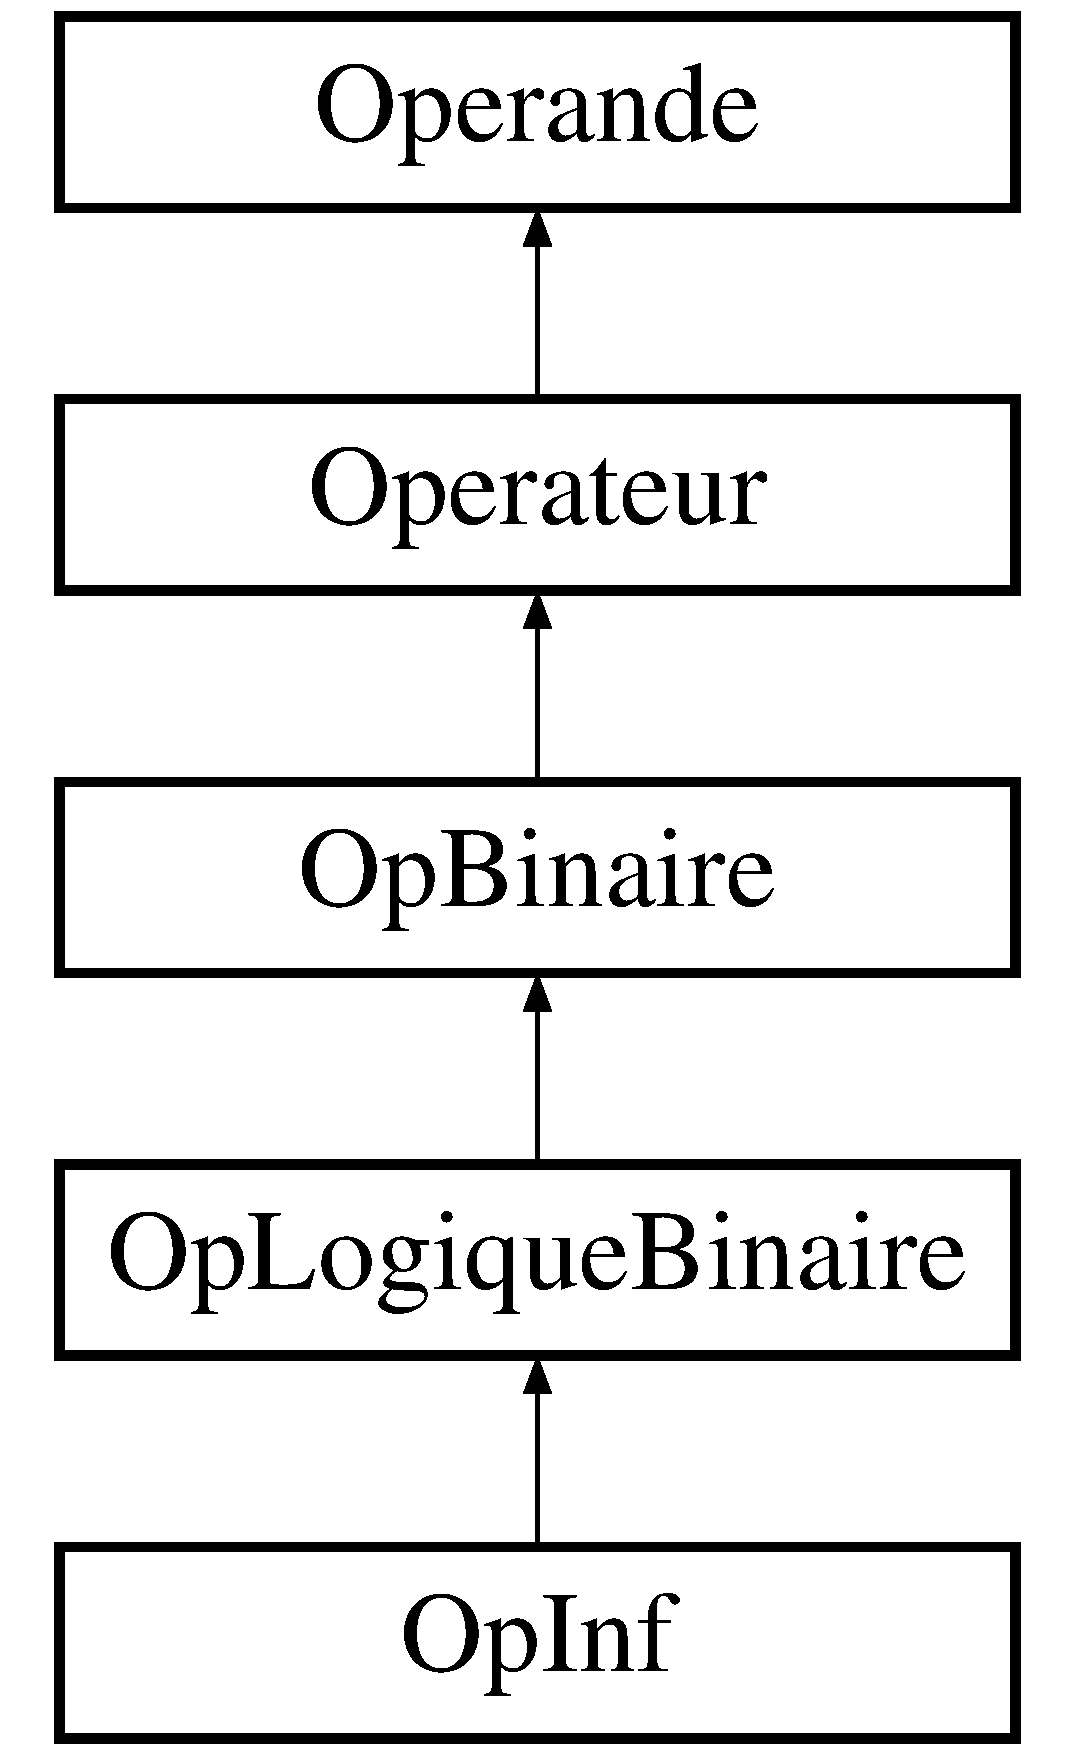
\includegraphics[height=5.000000cm]{class_op_inf}
\end{center}
\end{figure}
\subsection*{Public Member Functions}
\begin{DoxyCompactItemize}
\item 
\hyperlink{class_op_inf_a784e5bc4ceebc9f2b2897845382d82dc}{Op\+Inf} ()
\item 
\hyperlink{class_litterale}{Litterale} $\ast$ \hyperlink{class_op_inf_a45b7ab8190cdc2f45e2413d507a34e60}{action\+Logi\+Numerique} (\hyperlink{class_lit_numerique}{Lit\+Numerique} $\ast$arg1, \hyperlink{class_lit_numerique}{Lit\+Numerique} $\ast$arg2)
\end{DoxyCompactItemize}
\subsection*{Additional Inherited Members}


\subsection{Detailed Description}


Definition at line 19 of file operator\+Logique.\+h.



\subsection{Constructor \& Destructor Documentation}
\index{Op\+Inf@{Op\+Inf}!Op\+Inf@{Op\+Inf}}
\index{Op\+Inf@{Op\+Inf}!Op\+Inf@{Op\+Inf}}
\subsubsection[{\texorpdfstring{Op\+Inf()}{OpInf()}}]{\setlength{\rightskip}{0pt plus 5cm}Op\+Inf\+::\+Op\+Inf (
\begin{DoxyParamCaption}
{}
\end{DoxyParamCaption}
)\hspace{0.3cm}{\ttfamily [inline]}}\hypertarget{class_op_inf_a784e5bc4ceebc9f2b2897845382d82dc}{}\label{class_op_inf_a784e5bc4ceebc9f2b2897845382d82dc}


Definition at line 21 of file operator\+Logique.\+h.



\subsection{Member Function Documentation}
\index{Op\+Inf@{Op\+Inf}!action\+Logi\+Numerique@{action\+Logi\+Numerique}}
\index{action\+Logi\+Numerique@{action\+Logi\+Numerique}!Op\+Inf@{Op\+Inf}}
\subsubsection[{\texorpdfstring{action\+Logi\+Numerique(\+Lit\+Numerique $\ast$arg1, Lit\+Numerique $\ast$arg2)}{actionLogiNumerique(LitNumerique *arg1, LitNumerique *arg2)}}]{\setlength{\rightskip}{0pt plus 5cm}{\bf Litterale} $\ast$ Op\+Inf\+::action\+Logi\+Numerique (
\begin{DoxyParamCaption}
\item[{{\bf Lit\+Numerique} $\ast$}]{arg1, }
\item[{{\bf Lit\+Numerique} $\ast$}]{arg2}
\end{DoxyParamCaption}
)\hspace{0.3cm}{\ttfamily [virtual]}}\hypertarget{class_op_inf_a45b7ab8190cdc2f45e2413d507a34e60}{}\label{class_op_inf_a45b7ab8190cdc2f45e2413d507a34e60}


Implements \hyperlink{class_op_logique_binaire_a8fcab4c45ebcadbbcfecfa0c02e36f21}{Op\+Logique\+Binaire}.



Definition at line 32 of file operator\+Logique.\+cpp.



The documentation for this class was generated from the following files\+:\begin{DoxyCompactItemize}
\item 
\hyperlink{operator_logique_8h}{operator\+Logique.\+h}\item 
\hyperlink{operator_logique_8cpp}{operator\+Logique.\+cpp}\end{DoxyCompactItemize}

\hypertarget{class_op_infeg}{}\section{Op\+Infeg Class Reference}
\label{class_op_infeg}\index{Op\+Infeg@{Op\+Infeg}}


{\ttfamily \#include $<$operator\+Logique.\+h$>$}

Inheritance diagram for Op\+Infeg\+:\begin{figure}[H]
\begin{center}
\leavevmode
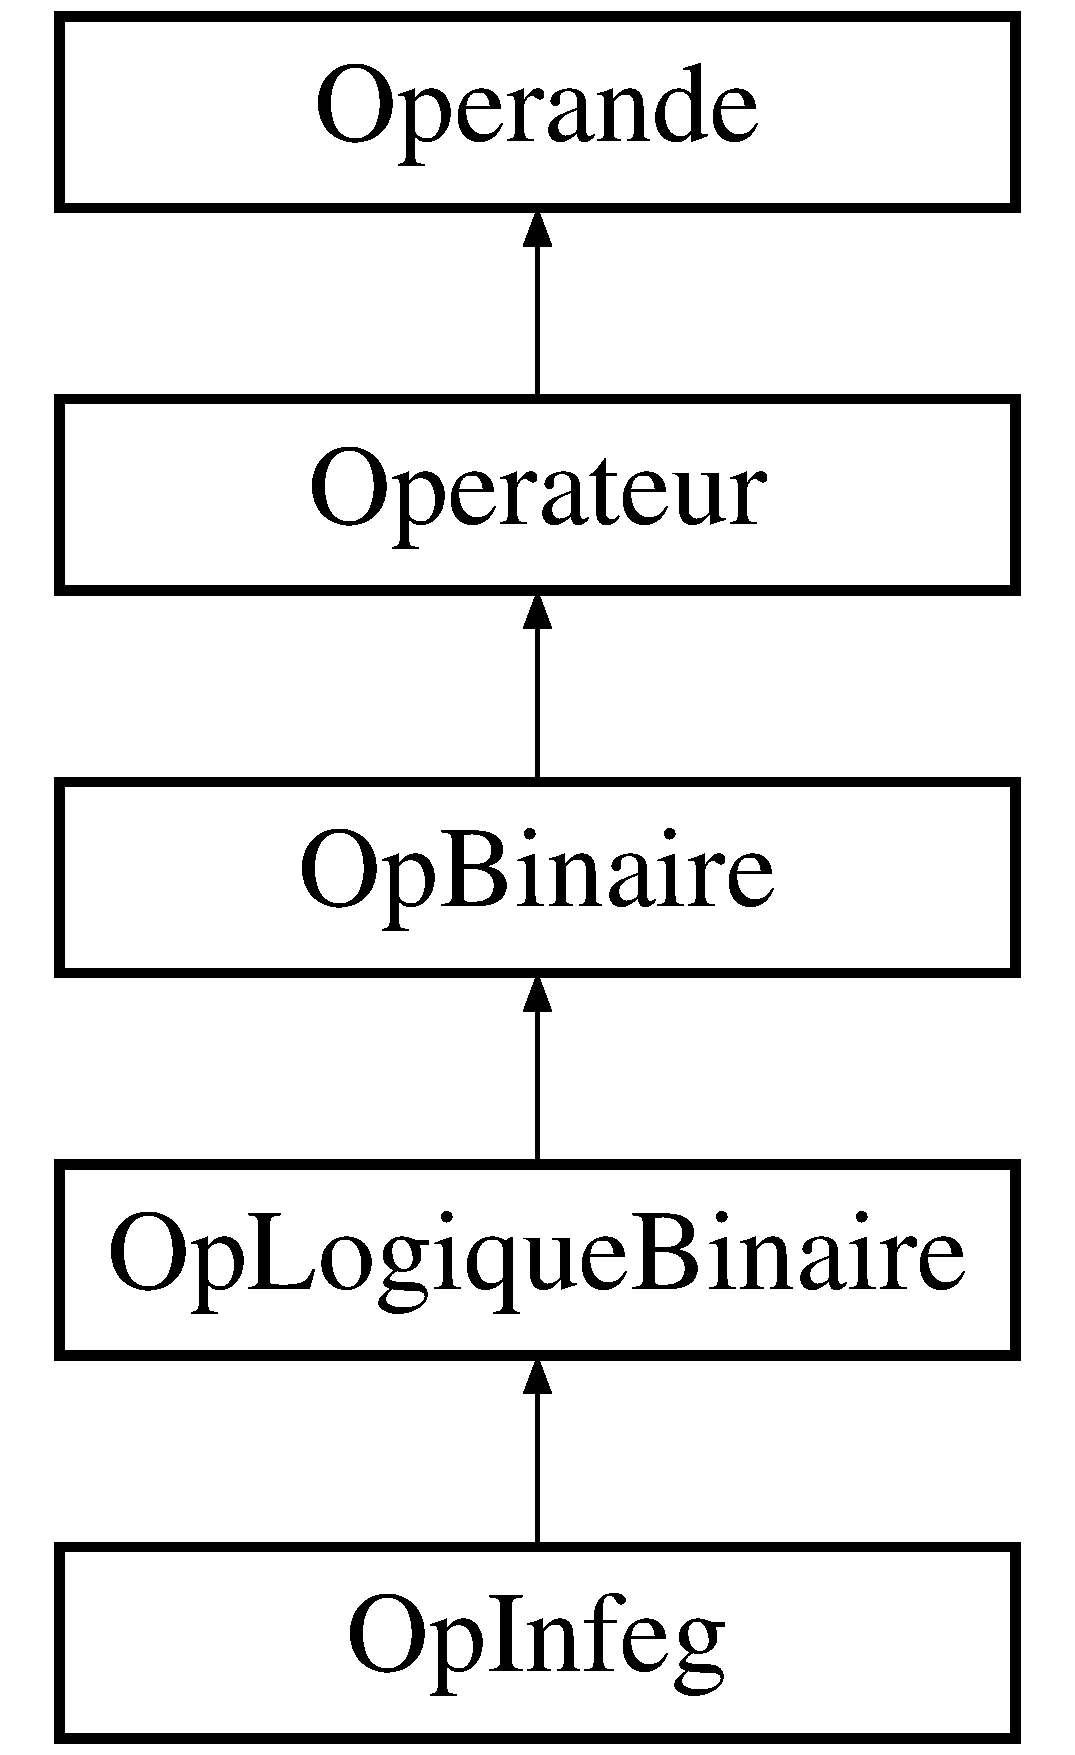
\includegraphics[height=5.000000cm]{class_op_infeg}
\end{center}
\end{figure}
\subsection*{Public Member Functions}
\begin{DoxyCompactItemize}
\item 
\hyperlink{class_op_infeg_a37caa0762a9fe7435f144e6414b4c26d}{Op\+Infeg} ()
\item 
\hyperlink{class_litterale}{Litterale} $\ast$ \hyperlink{class_op_infeg_ad1233fd7f991e78785e5578d97013ee8}{action\+Logi\+Numerique} (\hyperlink{class_lit_numerique}{Lit\+Numerique} $\ast$arg1, \hyperlink{class_lit_numerique}{Lit\+Numerique} $\ast$arg2)
\end{DoxyCompactItemize}
\subsection*{Additional Inherited Members}


\subsection{Detailed Description}


Definition at line 40 of file operator\+Logique.\+h.



\subsection{Constructor \& Destructor Documentation}
\index{Op\+Infeg@{Op\+Infeg}!Op\+Infeg@{Op\+Infeg}}
\index{Op\+Infeg@{Op\+Infeg}!Op\+Infeg@{Op\+Infeg}}
\subsubsection[{\texorpdfstring{Op\+Infeg()}{OpInfeg()}}]{\setlength{\rightskip}{0pt plus 5cm}Op\+Infeg\+::\+Op\+Infeg (
\begin{DoxyParamCaption}
{}
\end{DoxyParamCaption}
)\hspace{0.3cm}{\ttfamily [inline]}}\hypertarget{class_op_infeg_a37caa0762a9fe7435f144e6414b4c26d}{}\label{class_op_infeg_a37caa0762a9fe7435f144e6414b4c26d}


Definition at line 42 of file operator\+Logique.\+h.



\subsection{Member Function Documentation}
\index{Op\+Infeg@{Op\+Infeg}!action\+Logi\+Numerique@{action\+Logi\+Numerique}}
\index{action\+Logi\+Numerique@{action\+Logi\+Numerique}!Op\+Infeg@{Op\+Infeg}}
\subsubsection[{\texorpdfstring{action\+Logi\+Numerique(\+Lit\+Numerique $\ast$arg1, Lit\+Numerique $\ast$arg2)}{actionLogiNumerique(LitNumerique *arg1, LitNumerique *arg2)}}]{\setlength{\rightskip}{0pt plus 5cm}{\bf Litterale} $\ast$ Op\+Infeg\+::action\+Logi\+Numerique (
\begin{DoxyParamCaption}
\item[{{\bf Lit\+Numerique} $\ast$}]{arg1, }
\item[{{\bf Lit\+Numerique} $\ast$}]{arg2}
\end{DoxyParamCaption}
)\hspace{0.3cm}{\ttfamily [virtual]}}\hypertarget{class_op_infeg_ad1233fd7f991e78785e5578d97013ee8}{}\label{class_op_infeg_ad1233fd7f991e78785e5578d97013ee8}


Implements \hyperlink{class_op_logique_binaire_a8fcab4c45ebcadbbcfecfa0c02e36f21}{Op\+Logique\+Binaire}.



Definition at line 48 of file operator\+Logique.\+cpp.



The documentation for this class was generated from the following files\+:\begin{DoxyCompactItemize}
\item 
\hyperlink{operator_logique_8h}{operator\+Logique.\+h}\item 
\hyperlink{operator_logique_8cpp}{operator\+Logique.\+cpp}\end{DoxyCompactItemize}

\hypertarget{class_op_infeg_factory}{}\section{Op\+Infeg\+Factory Class Reference}
\label{class_op_infeg_factory}\index{Op\+Infeg\+Factory@{Op\+Infeg\+Factory}}


{\ttfamily \#include $<$operator\+Factory.\+h$>$}

Inheritance diagram for Op\+Infeg\+Factory\+:\begin{figure}[H]
\begin{center}
\leavevmode
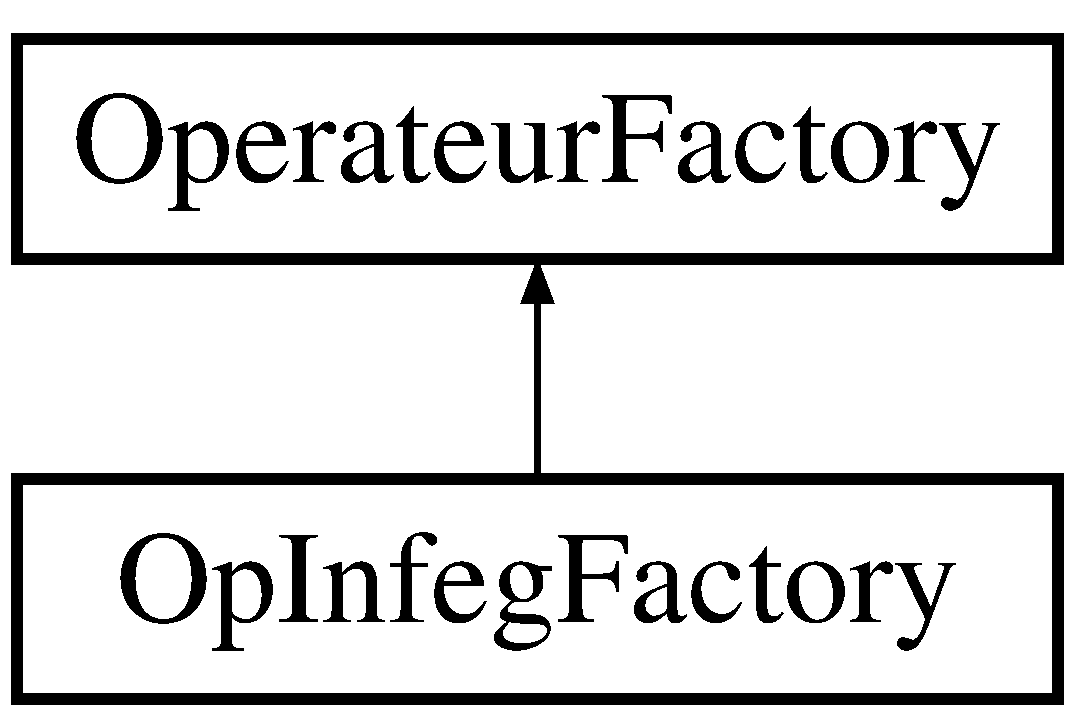
\includegraphics[height=2.000000cm]{class_op_infeg_factory}
\end{center}
\end{figure}
\subsection*{Public Member Functions}
\begin{DoxyCompactItemize}
\item 
\hyperlink{class_op_infeg_factory_af26e6dbb4162fff562b26dd54f3c7c97}{Op\+Infeg\+Factory} ()
\item 
\hyperlink{class_operateur}{Operateur} $\ast$ \hyperlink{class_op_infeg_factory_a3acf85e418fa861d09ca3272ae643ed5}{get\+Operateur} ()
\end{DoxyCompactItemize}
\subsection*{Additional Inherited Members}


\subsection{Detailed Description}


Definition at line 149 of file operator\+Factory.\+h.



\subsection{Constructor \& Destructor Documentation}
\index{Op\+Infeg\+Factory@{Op\+Infeg\+Factory}!Op\+Infeg\+Factory@{Op\+Infeg\+Factory}}
\index{Op\+Infeg\+Factory@{Op\+Infeg\+Factory}!Op\+Infeg\+Factory@{Op\+Infeg\+Factory}}
\subsubsection[{\texorpdfstring{Op\+Infeg\+Factory()}{OpInfegFactory()}}]{\setlength{\rightskip}{0pt plus 5cm}Op\+Infeg\+Factory\+::\+Op\+Infeg\+Factory (
\begin{DoxyParamCaption}
{}
\end{DoxyParamCaption}
)\hspace{0.3cm}{\ttfamily [inline]}}\hypertarget{class_op_infeg_factory_af26e6dbb4162fff562b26dd54f3c7c97}{}\label{class_op_infeg_factory_af26e6dbb4162fff562b26dd54f3c7c97}


Definition at line 151 of file operator\+Factory.\+h.



\subsection{Member Function Documentation}
\index{Op\+Infeg\+Factory@{Op\+Infeg\+Factory}!get\+Operateur@{get\+Operateur}}
\index{get\+Operateur@{get\+Operateur}!Op\+Infeg\+Factory@{Op\+Infeg\+Factory}}
\subsubsection[{\texorpdfstring{get\+Operateur()}{getOperateur()}}]{\setlength{\rightskip}{0pt plus 5cm}{\bf Operateur}$\ast$ Op\+Infeg\+Factory\+::get\+Operateur (
\begin{DoxyParamCaption}
{}
\end{DoxyParamCaption}
)\hspace{0.3cm}{\ttfamily [inline]}, {\ttfamily [virtual]}}\hypertarget{class_op_infeg_factory_a3acf85e418fa861d09ca3272ae643ed5}{}\label{class_op_infeg_factory_a3acf85e418fa861d09ca3272ae643ed5}


Implements \hyperlink{class_operateur_factory_aff61b2f67451f086d6abaea4231b2d78}{Operateur\+Factory}.



Definition at line 152 of file operator\+Factory.\+h.



The documentation for this class was generated from the following file\+:\begin{DoxyCompactItemize}
\item 
\hyperlink{operator_factory_8h}{operator\+Factory.\+h}\end{DoxyCompactItemize}

\hypertarget{class_op_inf_factory}{}\section{Op\+Inf\+Factory Class Reference}
\label{class_op_inf_factory}\index{Op\+Inf\+Factory@{Op\+Inf\+Factory}}


{\ttfamily \#include $<$operator\+Factory.\+h$>$}

Inheritance diagram for Op\+Inf\+Factory\+:\begin{figure}[H]
\begin{center}
\leavevmode
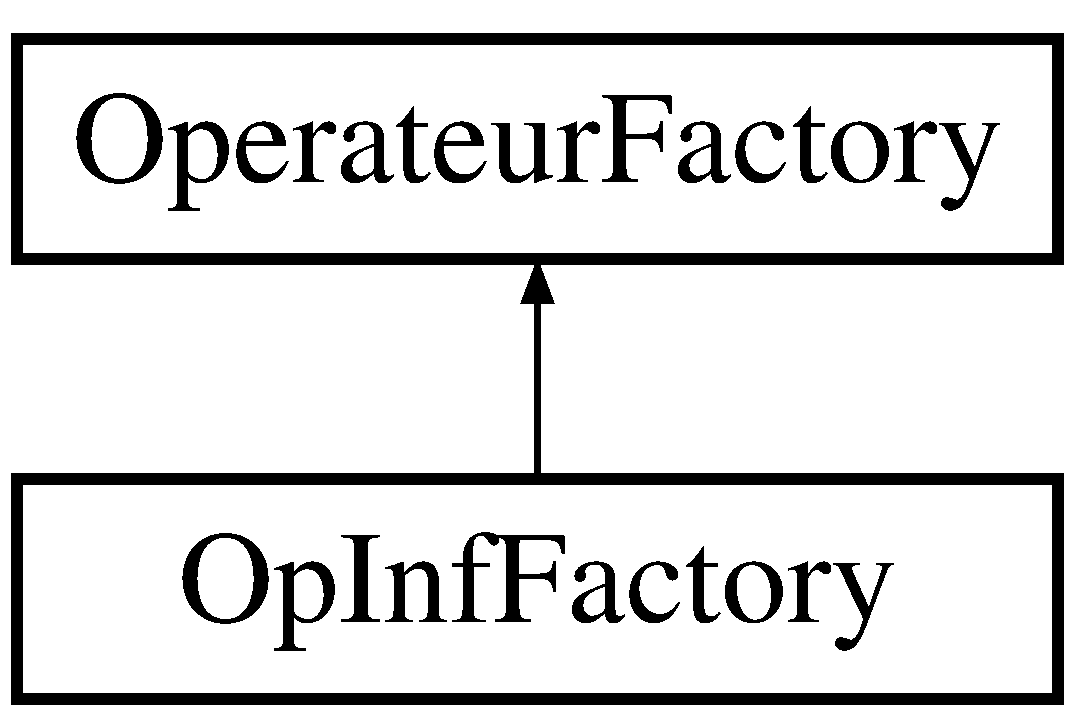
\includegraphics[height=2.000000cm]{class_op_inf_factory}
\end{center}
\end{figure}
\subsection*{Public Member Functions}
\begin{DoxyCompactItemize}
\item 
\hyperlink{class_op_inf_factory_aff1184d062dfa9ccdd996f04c564d323}{Op\+Inf\+Factory} ()
\item 
\hyperlink{class_operateur}{Operateur} $\ast$ \hyperlink{class_op_inf_factory_a981b37a05ef2f71278fa1a91b0e353d8}{get\+Operateur} ()
\end{DoxyCompactItemize}
\subsection*{Additional Inherited Members}


\subsection{Detailed Description}


Definition at line 161 of file operator\+Factory.\+h.



\subsection{Constructor \& Destructor Documentation}
\index{Op\+Inf\+Factory@{Op\+Inf\+Factory}!Op\+Inf\+Factory@{Op\+Inf\+Factory}}
\index{Op\+Inf\+Factory@{Op\+Inf\+Factory}!Op\+Inf\+Factory@{Op\+Inf\+Factory}}
\subsubsection[{\texorpdfstring{Op\+Inf\+Factory()}{OpInfFactory()}}]{\setlength{\rightskip}{0pt plus 5cm}Op\+Inf\+Factory\+::\+Op\+Inf\+Factory (
\begin{DoxyParamCaption}
{}
\end{DoxyParamCaption}
)\hspace{0.3cm}{\ttfamily [inline]}}\hypertarget{class_op_inf_factory_aff1184d062dfa9ccdd996f04c564d323}{}\label{class_op_inf_factory_aff1184d062dfa9ccdd996f04c564d323}


Definition at line 163 of file operator\+Factory.\+h.



\subsection{Member Function Documentation}
\index{Op\+Inf\+Factory@{Op\+Inf\+Factory}!get\+Operateur@{get\+Operateur}}
\index{get\+Operateur@{get\+Operateur}!Op\+Inf\+Factory@{Op\+Inf\+Factory}}
\subsubsection[{\texorpdfstring{get\+Operateur()}{getOperateur()}}]{\setlength{\rightskip}{0pt plus 5cm}{\bf Operateur}$\ast$ Op\+Inf\+Factory\+::get\+Operateur (
\begin{DoxyParamCaption}
{}
\end{DoxyParamCaption}
)\hspace{0.3cm}{\ttfamily [inline]}, {\ttfamily [virtual]}}\hypertarget{class_op_inf_factory_a981b37a05ef2f71278fa1a91b0e353d8}{}\label{class_op_inf_factory_a981b37a05ef2f71278fa1a91b0e353d8}


Implements \hyperlink{class_operateur_factory_aff61b2f67451f086d6abaea4231b2d78}{Operateur\+Factory}.



Definition at line 164 of file operator\+Factory.\+h.



The documentation for this class was generated from the following file\+:\begin{DoxyCompactItemize}
\item 
\hyperlink{operator_factory_8h}{operator\+Factory.\+h}\end{DoxyCompactItemize}

\hypertarget{class_op_ln}{}\section{Op\+Ln Class Reference}
\label{class_op_ln}\index{Op\+Ln@{Op\+Ln}}


{\ttfamily \#include $<$operator.\+h$>$}

Inheritance diagram for Op\+Ln\+:\begin{figure}[H]
\begin{center}
\leavevmode
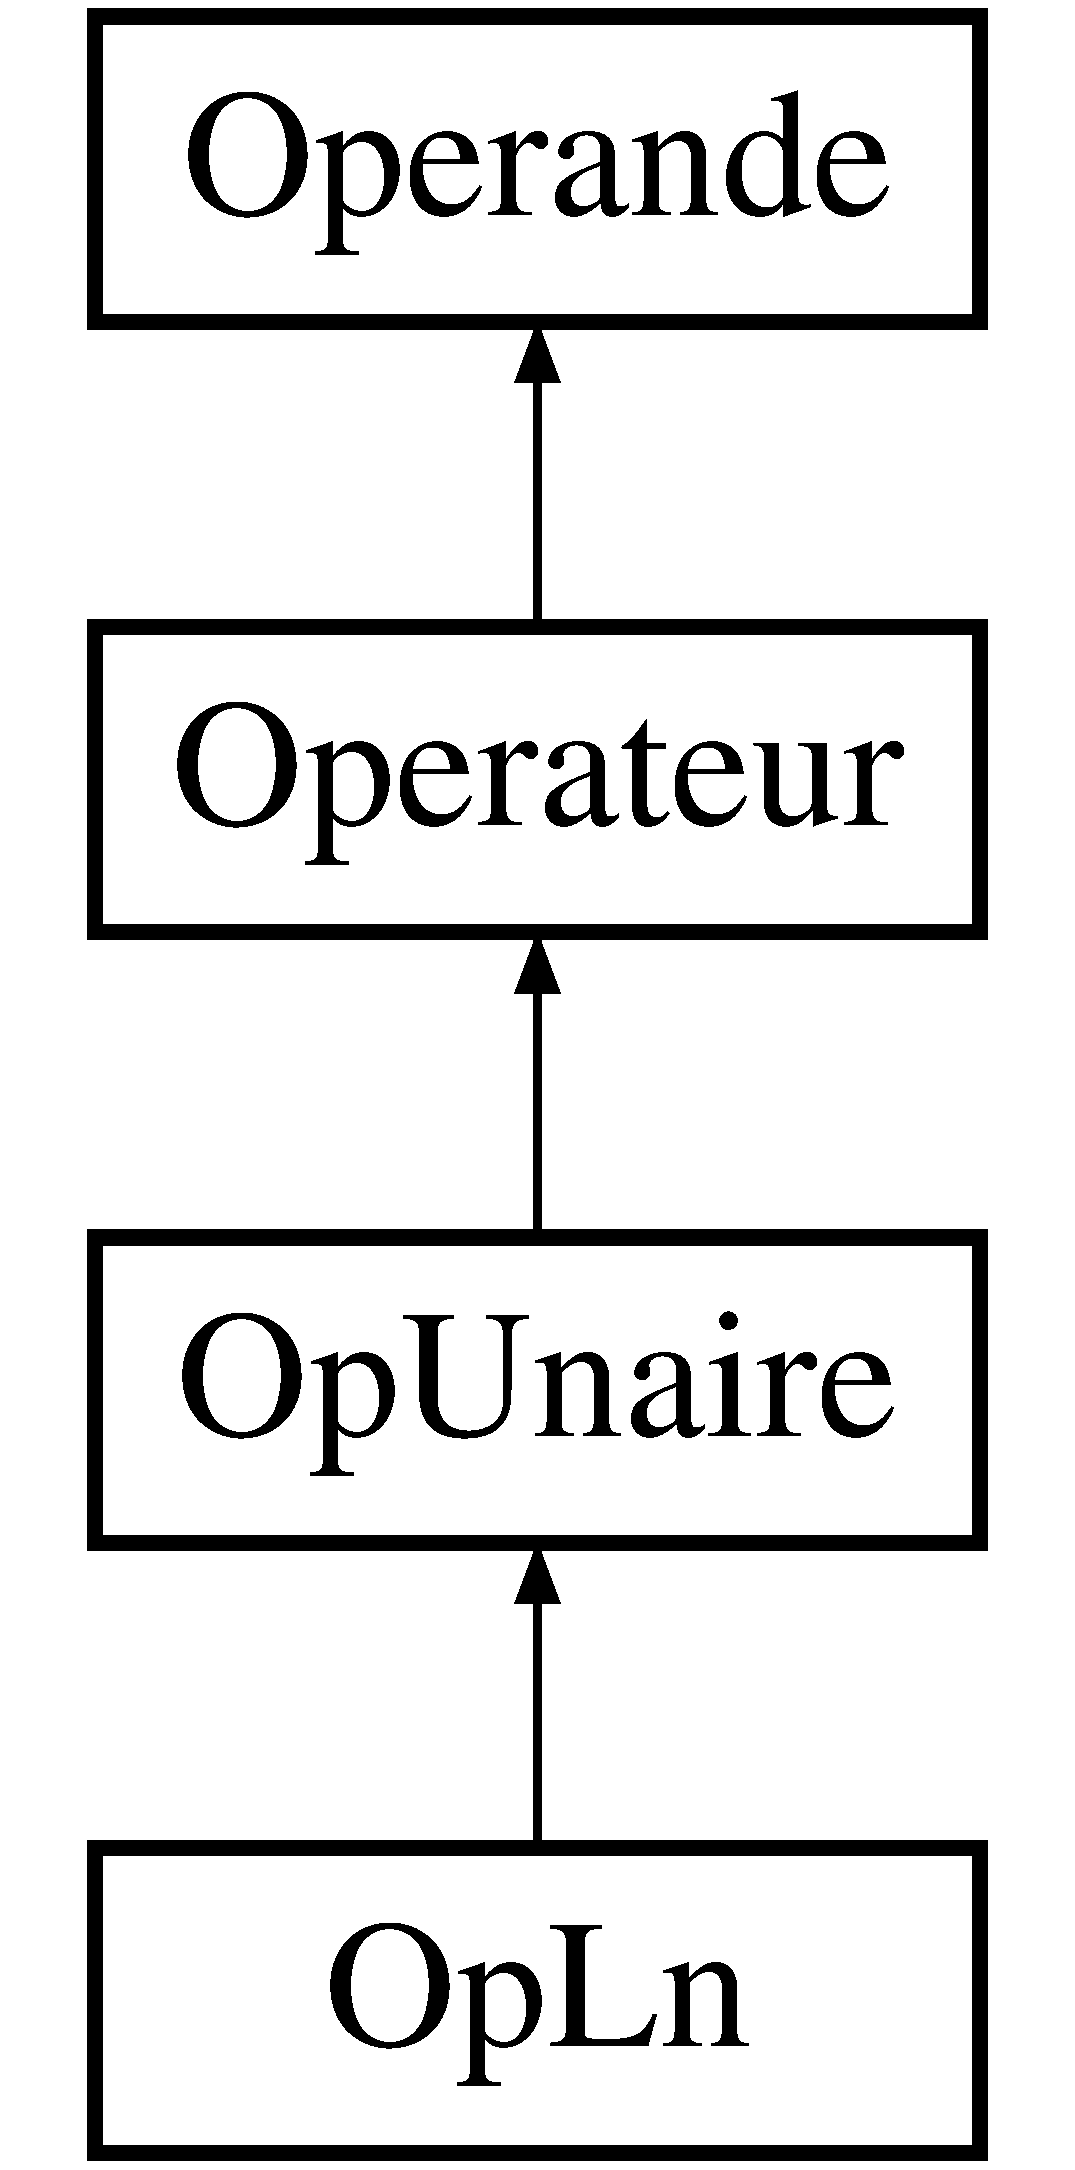
\includegraphics[height=4.000000cm]{class_op_ln}
\end{center}
\end{figure}
\subsection*{Public Member Functions}
\begin{DoxyCompactItemize}
\item 
\hyperlink{class_op_ln_a30eaaf55b82d7309ca24ff96a393919e}{Op\+Ln} ()
\item 
\hyperlink{class_litterale}{Litterale} $\ast$ \hyperlink{class_op_ln_af3ccbade0164af76ae941400b7bbe6ce}{action\+Num} (\hyperlink{class_entier}{Entier} \&arg1)
\item 
\hyperlink{class_litterale}{Litterale} $\ast$ \hyperlink{class_op_ln_a3fd161533906f6e658aa9cdc1512bd01}{action\+Num} (\hyperlink{class_reelle}{Reelle} \&arg1)
\item 
\hyperlink{class_litterale}{Litterale} $\ast$ \hyperlink{class_op_ln_abba32df08a1aad16a84eac0c95c9fd76}{action\+Num} (\hyperlink{class_rationnelle}{Rationnelle} \&arg1)
\end{DoxyCompactItemize}
\subsection*{Additional Inherited Members}


\subsection{Detailed Description}


Definition at line 72 of file operator.\+h.



\subsection{Constructor \& Destructor Documentation}
\index{Op\+Ln@{Op\+Ln}!Op\+Ln@{Op\+Ln}}
\index{Op\+Ln@{Op\+Ln}!Op\+Ln@{Op\+Ln}}
\subsubsection[{\texorpdfstring{Op\+Ln()}{OpLn()}}]{\setlength{\rightskip}{0pt plus 5cm}Op\+Ln\+::\+Op\+Ln (
\begin{DoxyParamCaption}
{}
\end{DoxyParamCaption}
)\hspace{0.3cm}{\ttfamily [inline]}}\hypertarget{class_op_ln_a30eaaf55b82d7309ca24ff96a393919e}{}\label{class_op_ln_a30eaaf55b82d7309ca24ff96a393919e}


Definition at line 74 of file operator.\+h.



\subsection{Member Function Documentation}
\index{Op\+Ln@{Op\+Ln}!action\+Num@{action\+Num}}
\index{action\+Num@{action\+Num}!Op\+Ln@{Op\+Ln}}
\subsubsection[{\texorpdfstring{action\+Num(\+Entier \&arg1)}{actionNum(Entier &arg1)}}]{\setlength{\rightskip}{0pt plus 5cm}{\bf Litterale} $\ast$ Op\+Ln\+::action\+Num (
\begin{DoxyParamCaption}
\item[{{\bf Entier} \&}]{arg1}
\end{DoxyParamCaption}
)\hspace{0.3cm}{\ttfamily [virtual]}}\hypertarget{class_op_ln_af3ccbade0164af76ae941400b7bbe6ce}{}\label{class_op_ln_af3ccbade0164af76ae941400b7bbe6ce}


Implements \hyperlink{class_op_unaire_a4db1c0cbd6ec4acbe89a6ef2ae68f901}{Op\+Unaire}.



Definition at line 134 of file operator.\+cpp.

\index{Op\+Ln@{Op\+Ln}!action\+Num@{action\+Num}}
\index{action\+Num@{action\+Num}!Op\+Ln@{Op\+Ln}}
\subsubsection[{\texorpdfstring{action\+Num(\+Reelle \&arg1)}{actionNum(Reelle &arg1)}}]{\setlength{\rightskip}{0pt plus 5cm}{\bf Litterale} $\ast$ Op\+Ln\+::action\+Num (
\begin{DoxyParamCaption}
\item[{{\bf Reelle} \&}]{arg1}
\end{DoxyParamCaption}
)\hspace{0.3cm}{\ttfamily [virtual]}}\hypertarget{class_op_ln_a3fd161533906f6e658aa9cdc1512bd01}{}\label{class_op_ln_a3fd161533906f6e658aa9cdc1512bd01}


Implements \hyperlink{class_op_unaire_a0b92d632cf248e765783f23d6d637d1f}{Op\+Unaire}.



Definition at line 140 of file operator.\+cpp.

\index{Op\+Ln@{Op\+Ln}!action\+Num@{action\+Num}}
\index{action\+Num@{action\+Num}!Op\+Ln@{Op\+Ln}}
\subsubsection[{\texorpdfstring{action\+Num(\+Rationnelle \&arg1)}{actionNum(Rationnelle &arg1)}}]{\setlength{\rightskip}{0pt plus 5cm}{\bf Litterale} $\ast$ Op\+Ln\+::action\+Num (
\begin{DoxyParamCaption}
\item[{{\bf Rationnelle} \&}]{arg1}
\end{DoxyParamCaption}
)\hspace{0.3cm}{\ttfamily [virtual]}}\hypertarget{class_op_ln_abba32df08a1aad16a84eac0c95c9fd76}{}\label{class_op_ln_abba32df08a1aad16a84eac0c95c9fd76}


Implements \hyperlink{class_op_unaire_a7728e3d41bfe8ace1f9343a4cd404502}{Op\+Unaire}.



Definition at line 146 of file operator.\+cpp.



The documentation for this class was generated from the following files\+:\begin{DoxyCompactItemize}
\item 
\hyperlink{operator_8h}{operator.\+h}\item 
\hyperlink{operator_8cpp}{operator.\+cpp}\end{DoxyCompactItemize}

\hypertarget{class_op_ln_factory}{}\section{Op\+Ln\+Factory Class Reference}
\label{class_op_ln_factory}\index{Op\+Ln\+Factory@{Op\+Ln\+Factory}}


{\ttfamily \#include $<$operator\+Factory.\+h$>$}

Inheritance diagram for Op\+Ln\+Factory\+:\begin{figure}[H]
\begin{center}
\leavevmode
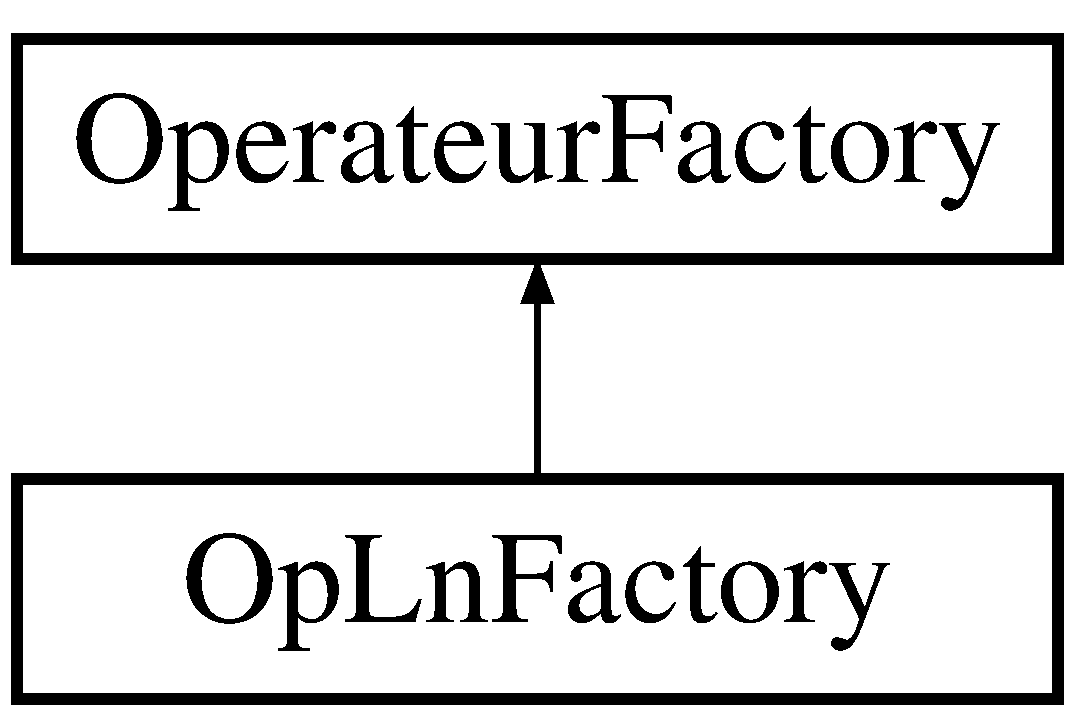
\includegraphics[height=2.000000cm]{class_op_ln_factory}
\end{center}
\end{figure}
\subsection*{Public Member Functions}
\begin{DoxyCompactItemize}
\item 
\hyperlink{class_op_ln_factory_ab1e59f3d5da2ef6166e874b051101c56}{Op\+Ln\+Factory} ()
\item 
\hyperlink{class_operateur}{Operateur} $\ast$ \hyperlink{class_op_ln_factory_a9634e94728f2ea42f08cc84b40e36629}{get\+Operateur} ()
\end{DoxyCompactItemize}
\subsection*{Additional Inherited Members}


\subsection{Detailed Description}


Definition at line 27 of file operator\+Factory.\+h.



\subsection{Constructor \& Destructor Documentation}
\index{Op\+Ln\+Factory@{Op\+Ln\+Factory}!Op\+Ln\+Factory@{Op\+Ln\+Factory}}
\index{Op\+Ln\+Factory@{Op\+Ln\+Factory}!Op\+Ln\+Factory@{Op\+Ln\+Factory}}
\subsubsection[{\texorpdfstring{Op\+Ln\+Factory()}{OpLnFactory()}}]{\setlength{\rightskip}{0pt plus 5cm}Op\+Ln\+Factory\+::\+Op\+Ln\+Factory (
\begin{DoxyParamCaption}
{}
\end{DoxyParamCaption}
)\hspace{0.3cm}{\ttfamily [inline]}}\hypertarget{class_op_ln_factory_ab1e59f3d5da2ef6166e874b051101c56}{}\label{class_op_ln_factory_ab1e59f3d5da2ef6166e874b051101c56}


Definition at line 29 of file operator\+Factory.\+h.



\subsection{Member Function Documentation}
\index{Op\+Ln\+Factory@{Op\+Ln\+Factory}!get\+Operateur@{get\+Operateur}}
\index{get\+Operateur@{get\+Operateur}!Op\+Ln\+Factory@{Op\+Ln\+Factory}}
\subsubsection[{\texorpdfstring{get\+Operateur()}{getOperateur()}}]{\setlength{\rightskip}{0pt plus 5cm}{\bf Operateur}$\ast$ Op\+Ln\+Factory\+::get\+Operateur (
\begin{DoxyParamCaption}
{}
\end{DoxyParamCaption}
)\hspace{0.3cm}{\ttfamily [inline]}, {\ttfamily [virtual]}}\hypertarget{class_op_ln_factory_a9634e94728f2ea42f08cc84b40e36629}{}\label{class_op_ln_factory_a9634e94728f2ea42f08cc84b40e36629}


Implements \hyperlink{class_operateur_factory_aff61b2f67451f086d6abaea4231b2d78}{Operateur\+Factory}.



Definition at line 30 of file operator\+Factory.\+h.



The documentation for this class was generated from the following file\+:\begin{DoxyCompactItemize}
\item 
\hyperlink{operator_factory_8h}{operator\+Factory.\+h}\end{DoxyCompactItemize}

\hypertarget{class_op_logique_binaire}{}\section{Op\+Logique\+Binaire Class Reference}
\label{class_op_logique_binaire}\index{Op\+Logique\+Binaire@{Op\+Logique\+Binaire}}


{\ttfamily \#include $<$operator\+Logique.\+h$>$}

Inheritance diagram for Op\+Logique\+Binaire\+:\begin{figure}[H]
\begin{center}
\leavevmode
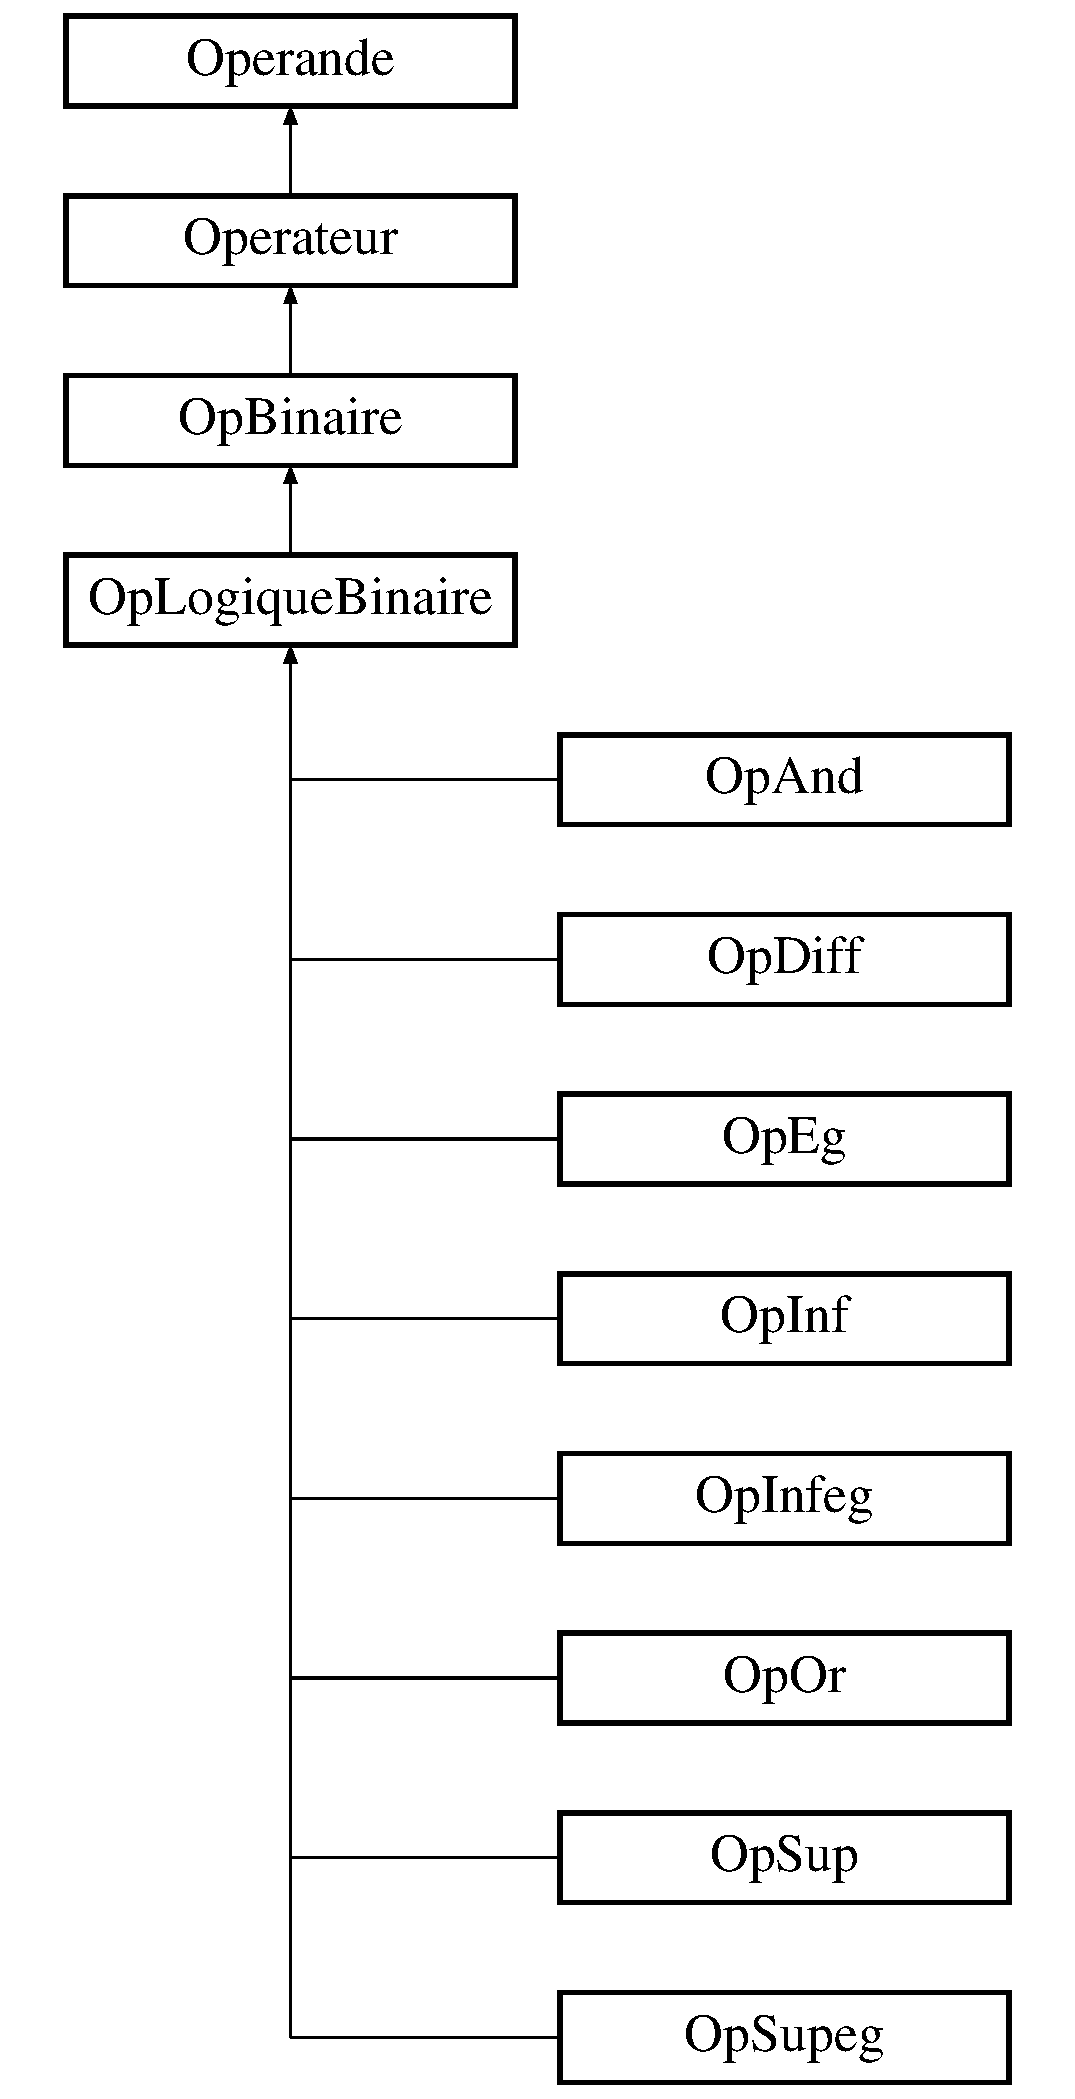
\includegraphics[height=12.000000cm]{class_op_logique_binaire}
\end{center}
\end{figure}
\subsection*{Public Member Functions}
\begin{DoxyCompactItemize}
\item 
\hyperlink{class_op_logique_binaire_a591334b408deef00d85f3515ddbb6af7}{Op\+Logique\+Binaire} (const Q\+String \&na)
\item 
virtual \hyperlink{class_op_logique_binaire_ad3361dea367bf9e7d0acd597e34e5b4d}{$\sim$\+Op\+Logique\+Binaire} ()
\item 
\hyperlink{class_litterale}{Litterale} $\ast$ \hyperlink{class_op_logique_binaire_a5565bc1dd13c6bddea8b91995dda703a}{fonction\+Num} (\hyperlink{class_nombres}{Nombres} $\ast$arg1, \hyperlink{class_litterale}{Litterale} $\ast$arg2)
\item 
\hyperlink{class_litterale}{Litterale} $\ast$ \hyperlink{class_op_logique_binaire_a4fbde2ff67fe7f2bfa1898522158bff1}{fonction\+Expression} (\hyperlink{class_lit_expression}{Lit\+Expression} $\ast$arg1, \hyperlink{class_litterale}{Litterale} $\ast$arg2)
\item 
virtual \hyperlink{class_litterale}{Litterale} $\ast$ \hyperlink{class_op_logique_binaire_a8fcab4c45ebcadbbcfecfa0c02e36f21}{action\+Logi\+Numerique} (\hyperlink{class_lit_numerique}{Lit\+Numerique} $\ast$arg1, \hyperlink{class_lit_numerique}{Lit\+Numerique} $\ast$arg2)=0
\end{DoxyCompactItemize}
\subsection*{Additional Inherited Members}


\subsection{Detailed Description}


Definition at line 8 of file operator\+Logique.\+h.



\subsection{Constructor \& Destructor Documentation}
\index{Op\+Logique\+Binaire@{Op\+Logique\+Binaire}!Op\+Logique\+Binaire@{Op\+Logique\+Binaire}}
\index{Op\+Logique\+Binaire@{Op\+Logique\+Binaire}!Op\+Logique\+Binaire@{Op\+Logique\+Binaire}}
\subsubsection[{\texorpdfstring{Op\+Logique\+Binaire(const Q\+String \&na)}{OpLogiqueBinaire(const QString &na)}}]{\setlength{\rightskip}{0pt plus 5cm}Op\+Logique\+Binaire\+::\+Op\+Logique\+Binaire (
\begin{DoxyParamCaption}
\item[{const Q\+String \&}]{na}
\end{DoxyParamCaption}
)\hspace{0.3cm}{\ttfamily [inline]}}\hypertarget{class_op_logique_binaire_a591334b408deef00d85f3515ddbb6af7}{}\label{class_op_logique_binaire_a591334b408deef00d85f3515ddbb6af7}


Definition at line 10 of file operator\+Logique.\+h.

\index{Op\+Logique\+Binaire@{Op\+Logique\+Binaire}!````~Op\+Logique\+Binaire@{$\sim$\+Op\+Logique\+Binaire}}
\index{````~Op\+Logique\+Binaire@{$\sim$\+Op\+Logique\+Binaire}!Op\+Logique\+Binaire@{Op\+Logique\+Binaire}}
\subsubsection[{\texorpdfstring{$\sim$\+Op\+Logique\+Binaire()}{~OpLogiqueBinaire()}}]{\setlength{\rightskip}{0pt plus 5cm}Op\+Logique\+Binaire\+::$\sim$\+Op\+Logique\+Binaire (
\begin{DoxyParamCaption}
{}
\end{DoxyParamCaption}
)\hspace{0.3cm}{\ttfamily [virtual]}}\hypertarget{class_op_logique_binaire_ad3361dea367bf9e7d0acd597e34e5b4d}{}\label{class_op_logique_binaire_ad3361dea367bf9e7d0acd597e34e5b4d}


Definition at line 4 of file operator\+Logique.\+cpp.



\subsection{Member Function Documentation}
\index{Op\+Logique\+Binaire@{Op\+Logique\+Binaire}!action\+Logi\+Numerique@{action\+Logi\+Numerique}}
\index{action\+Logi\+Numerique@{action\+Logi\+Numerique}!Op\+Logique\+Binaire@{Op\+Logique\+Binaire}}
\subsubsection[{\texorpdfstring{action\+Logi\+Numerique(\+Lit\+Numerique $\ast$arg1, Lit\+Numerique $\ast$arg2)=0}{actionLogiNumerique(LitNumerique *arg1, LitNumerique *arg2)=0}}]{\setlength{\rightskip}{0pt plus 5cm}virtual {\bf Litterale}$\ast$ Op\+Logique\+Binaire\+::action\+Logi\+Numerique (
\begin{DoxyParamCaption}
\item[{{\bf Lit\+Numerique} $\ast$}]{arg1, }
\item[{{\bf Lit\+Numerique} $\ast$}]{arg2}
\end{DoxyParamCaption}
)\hspace{0.3cm}{\ttfamily [pure virtual]}}\hypertarget{class_op_logique_binaire_a8fcab4c45ebcadbbcfecfa0c02e36f21}{}\label{class_op_logique_binaire_a8fcab4c45ebcadbbcfecfa0c02e36f21}


Implemented in \hyperlink{class_op_or_ad2fe1c5e10d965fb3292bb2b41ba1a70}{Op\+Or}, \hyperlink{class_op_and_a84274acf7a0d4e48ff11a9683d488808}{Op\+And}, \hyperlink{class_op_diff_aa863ce6389c18a0546f6b1b6aae4d9dd}{Op\+Diff}, \hyperlink{class_op_eg_ab84762131924ea6ca5e60960593411e0}{Op\+Eg}, \hyperlink{class_op_infeg_ad1233fd7f991e78785e5578d97013ee8}{Op\+Infeg}, \hyperlink{class_op_supeg_a4a8860fa49a17f4d42e97f85c407b817}{Op\+Supeg}, \hyperlink{class_op_sup_a33bd87ca89fbea101345338ef37aee06}{Op\+Sup}, and \hyperlink{class_op_inf_a45b7ab8190cdc2f45e2413d507a34e60}{Op\+Inf}.

\index{Op\+Logique\+Binaire@{Op\+Logique\+Binaire}!fonction\+Expression@{fonction\+Expression}}
\index{fonction\+Expression@{fonction\+Expression}!Op\+Logique\+Binaire@{Op\+Logique\+Binaire}}
\subsubsection[{\texorpdfstring{fonction\+Expression(\+Lit\+Expression $\ast$arg1, Litterale $\ast$arg2)}{fonctionExpression(LitExpression *arg1, Litterale *arg2)}}]{\setlength{\rightskip}{0pt plus 5cm}{\bf Litterale} $\ast$ Op\+Logique\+Binaire\+::fonction\+Expression (
\begin{DoxyParamCaption}
\item[{{\bf Lit\+Expression} $\ast$}]{arg1, }
\item[{{\bf Litterale} $\ast$}]{arg2}
\end{DoxyParamCaption}
)\hspace{0.3cm}{\ttfamily [virtual]}}\hypertarget{class_op_logique_binaire_a4fbde2ff67fe7f2bfa1898522158bff1}{}\label{class_op_logique_binaire_a4fbde2ff67fe7f2bfa1898522158bff1}


Implements \hyperlink{class_op_binaire_a72ea45bf3157516edeca687668d83b32}{Op\+Binaire}.



Definition at line 13 of file operator\+Logique.\+cpp.

\index{Op\+Logique\+Binaire@{Op\+Logique\+Binaire}!fonction\+Num@{fonction\+Num}}
\index{fonction\+Num@{fonction\+Num}!Op\+Logique\+Binaire@{Op\+Logique\+Binaire}}
\subsubsection[{\texorpdfstring{fonction\+Num(\+Nombres $\ast$arg1, Litterale $\ast$arg2)}{fonctionNum(Nombres *arg1, Litterale *arg2)}}]{\setlength{\rightskip}{0pt plus 5cm}{\bf Litterale} $\ast$ Op\+Logique\+Binaire\+::fonction\+Num (
\begin{DoxyParamCaption}
\item[{{\bf Nombres} $\ast$}]{arg1, }
\item[{{\bf Litterale} $\ast$}]{arg2}
\end{DoxyParamCaption}
)\hspace{0.3cm}{\ttfamily [virtual]}}\hypertarget{class_op_logique_binaire_a5565bc1dd13c6bddea8b91995dda703a}{}\label{class_op_logique_binaire_a5565bc1dd13c6bddea8b91995dda703a}


Implements \hyperlink{class_op_binaire_afb16dbd5f455b97afb5c07fae29b94fc}{Op\+Binaire}.



Definition at line 6 of file operator\+Logique.\+cpp.



The documentation for this class was generated from the following files\+:\begin{DoxyCompactItemize}
\item 
\hyperlink{operator_logique_8h}{operator\+Logique.\+h}\item 
\hyperlink{operator_logique_8cpp}{operator\+Logique.\+cpp}\end{DoxyCompactItemize}

\hypertarget{class_op_logique_unaire}{}\section{Op\+Logique\+Unaire Class Reference}
\label{class_op_logique_unaire}\index{Op\+Logique\+Unaire@{Op\+Logique\+Unaire}}


{\ttfamily \#include $<$operator.\+h$>$}

Inheritance diagram for Op\+Logique\+Unaire\+:\begin{figure}[H]
\begin{center}
\leavevmode
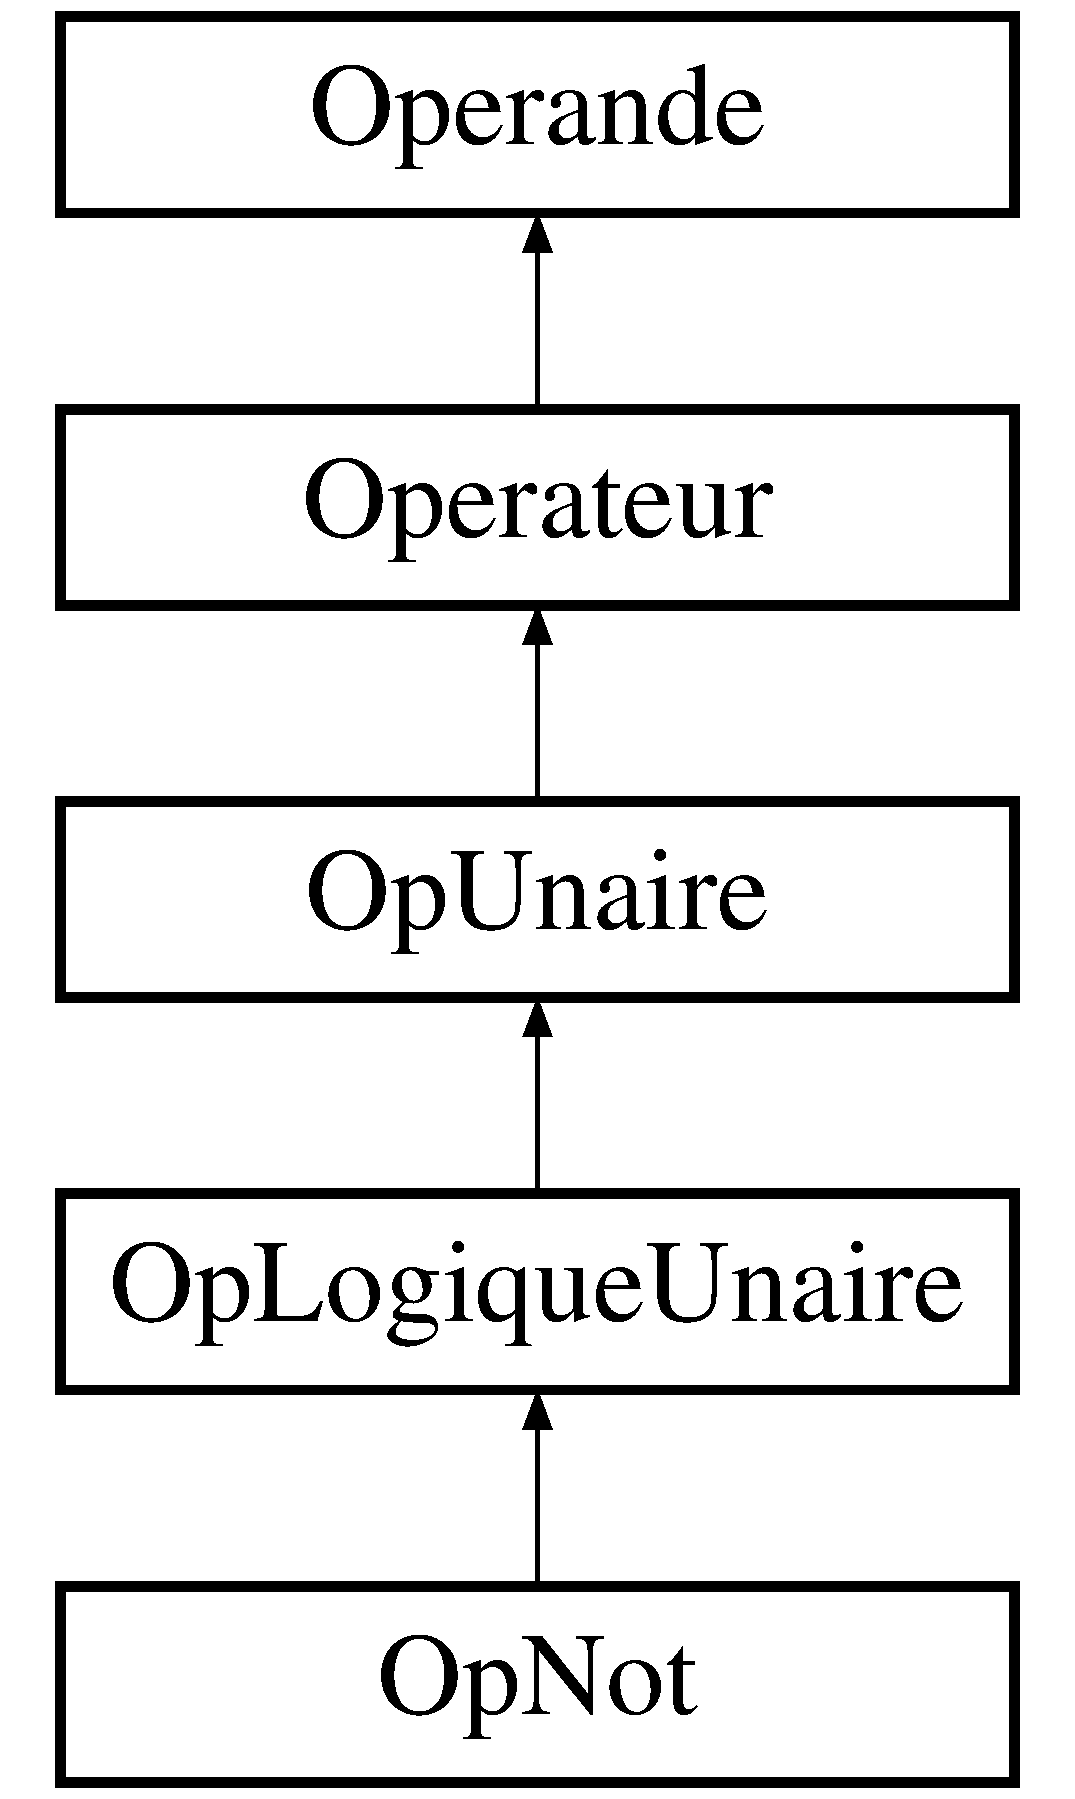
\includegraphics[height=5.000000cm]{class_op_logique_unaire}
\end{center}
\end{figure}
\subsection*{Public Member Functions}
\begin{DoxyCompactItemize}
\item 
\hyperlink{class_op_logique_unaire_a05ee8fc13b4f1b1b6b0eb242e8db608a}{Op\+Logique\+Unaire} (const Q\+String \&na)
\item 
virtual \hyperlink{class_op_logique_unaire_a536c88af3cfc8df1e6d0b1b37a42e3b8}{$\sim$\+Op\+Logique\+Unaire} ()
\item 
\hyperlink{class_litterale}{Litterale} $\ast$ \hyperlink{class_op_logique_unaire_a823d44ca7bb4caf3b9b34e3ff263001b}{fonction\+Num} (\hyperlink{class_nombres}{Nombres} $\ast$arg1)
\item 
virtual \hyperlink{class_litterale}{Litterale} $\ast$ \hyperlink{class_op_logique_unaire_a89c5a27b3dc232cf69aa1631231c3fc6}{action\+Logi\+Numerique} (\hyperlink{class_lit_numerique}{Lit\+Numerique} $\ast$arg1)=0
\item 
\hyperlink{class_litterale}{Litterale} $\ast$ \hyperlink{class_op_logique_unaire_a58809367f9cd3dbb4c0f3d66c21428c0}{action\+Num} (\hyperlink{class_reelle}{Reelle} \&arg1)
\item 
\hyperlink{class_litterale}{Litterale} $\ast$ \hyperlink{class_op_logique_unaire_a396bd51e071632ec4e607473068e1a62}{action\+Num} (\hyperlink{class_entier}{Entier} \&arg1)
\item 
\hyperlink{class_litterale}{Litterale} $\ast$ \hyperlink{class_op_logique_unaire_aa6c63a7c5b288d3c9e7d194453f4cffe}{action\+Num} (\hyperlink{class_rationnelle}{Rationnelle} \&arg1)
\end{DoxyCompactItemize}
\subsection*{Additional Inherited Members}


\subsection{Detailed Description}


Definition at line 43 of file operator.\+h.



\subsection{Constructor \& Destructor Documentation}
\index{Op\+Logique\+Unaire@{Op\+Logique\+Unaire}!Op\+Logique\+Unaire@{Op\+Logique\+Unaire}}
\index{Op\+Logique\+Unaire@{Op\+Logique\+Unaire}!Op\+Logique\+Unaire@{Op\+Logique\+Unaire}}
\subsubsection[{\texorpdfstring{Op\+Logique\+Unaire(const Q\+String \&na)}{OpLogiqueUnaire(const QString &na)}}]{\setlength{\rightskip}{0pt plus 5cm}Op\+Logique\+Unaire\+::\+Op\+Logique\+Unaire (
\begin{DoxyParamCaption}
\item[{const Q\+String \&}]{na}
\end{DoxyParamCaption}
)\hspace{0.3cm}{\ttfamily [inline]}}\hypertarget{class_op_logique_unaire_a05ee8fc13b4f1b1b6b0eb242e8db608a}{}\label{class_op_logique_unaire_a05ee8fc13b4f1b1b6b0eb242e8db608a}


Definition at line 45 of file operator.\+h.

\index{Op\+Logique\+Unaire@{Op\+Logique\+Unaire}!````~Op\+Logique\+Unaire@{$\sim$\+Op\+Logique\+Unaire}}
\index{````~Op\+Logique\+Unaire@{$\sim$\+Op\+Logique\+Unaire}!Op\+Logique\+Unaire@{Op\+Logique\+Unaire}}
\subsubsection[{\texorpdfstring{$\sim$\+Op\+Logique\+Unaire()}{~OpLogiqueUnaire()}}]{\setlength{\rightskip}{0pt plus 5cm}Op\+Logique\+Unaire\+::$\sim$\+Op\+Logique\+Unaire (
\begin{DoxyParamCaption}
{}
\end{DoxyParamCaption}
)\hspace{0.3cm}{\ttfamily [virtual]}}\hypertarget{class_op_logique_unaire_a536c88af3cfc8df1e6d0b1b37a42e3b8}{}\label{class_op_logique_unaire_a536c88af3cfc8df1e6d0b1b37a42e3b8}


Definition at line 188 of file operator.\+cpp.



\subsection{Member Function Documentation}
\index{Op\+Logique\+Unaire@{Op\+Logique\+Unaire}!action\+Logi\+Numerique@{action\+Logi\+Numerique}}
\index{action\+Logi\+Numerique@{action\+Logi\+Numerique}!Op\+Logique\+Unaire@{Op\+Logique\+Unaire}}
\subsubsection[{\texorpdfstring{action\+Logi\+Numerique(\+Lit\+Numerique $\ast$arg1)=0}{actionLogiNumerique(LitNumerique *arg1)=0}}]{\setlength{\rightskip}{0pt plus 5cm}virtual {\bf Litterale}$\ast$ Op\+Logique\+Unaire\+::action\+Logi\+Numerique (
\begin{DoxyParamCaption}
\item[{{\bf Lit\+Numerique} $\ast$}]{arg1}
\end{DoxyParamCaption}
)\hspace{0.3cm}{\ttfamily [pure virtual]}}\hypertarget{class_op_logique_unaire_a89c5a27b3dc232cf69aa1631231c3fc6}{}\label{class_op_logique_unaire_a89c5a27b3dc232cf69aa1631231c3fc6}


Implemented in \hyperlink{class_op_not_ad4a6fdf0a1de9ee9d41d87db5e872604}{Op\+Not}.

\index{Op\+Logique\+Unaire@{Op\+Logique\+Unaire}!action\+Num@{action\+Num}}
\index{action\+Num@{action\+Num}!Op\+Logique\+Unaire@{Op\+Logique\+Unaire}}
\subsubsection[{\texorpdfstring{action\+Num(\+Reelle \&arg1)}{actionNum(Reelle &arg1)}}]{\setlength{\rightskip}{0pt plus 5cm}{\bf Litterale} $\ast$ Op\+Logique\+Unaire\+::action\+Num (
\begin{DoxyParamCaption}
\item[{{\bf Reelle} \&}]{arg1}
\end{DoxyParamCaption}
)\hspace{0.3cm}{\ttfamily [virtual]}}\hypertarget{class_op_logique_unaire_a58809367f9cd3dbb4c0f3d66c21428c0}{}\label{class_op_logique_unaire_a58809367f9cd3dbb4c0f3d66c21428c0}


Implements \hyperlink{class_op_unaire_a0b92d632cf248e765783f23d6d637d1f}{Op\+Unaire}.



Definition at line 197 of file operator.\+cpp.

\index{Op\+Logique\+Unaire@{Op\+Logique\+Unaire}!action\+Num@{action\+Num}}
\index{action\+Num@{action\+Num}!Op\+Logique\+Unaire@{Op\+Logique\+Unaire}}
\subsubsection[{\texorpdfstring{action\+Num(\+Entier \&arg1)}{actionNum(Entier &arg1)}}]{\setlength{\rightskip}{0pt plus 5cm}{\bf Litterale} $\ast$ Op\+Logique\+Unaire\+::action\+Num (
\begin{DoxyParamCaption}
\item[{{\bf Entier} \&}]{arg1}
\end{DoxyParamCaption}
)\hspace{0.3cm}{\ttfamily [virtual]}}\hypertarget{class_op_logique_unaire_a396bd51e071632ec4e607473068e1a62}{}\label{class_op_logique_unaire_a396bd51e071632ec4e607473068e1a62}


Implements \hyperlink{class_op_unaire_a4db1c0cbd6ec4acbe89a6ef2ae68f901}{Op\+Unaire}.



Definition at line 196 of file operator.\+cpp.

\index{Op\+Logique\+Unaire@{Op\+Logique\+Unaire}!action\+Num@{action\+Num}}
\index{action\+Num@{action\+Num}!Op\+Logique\+Unaire@{Op\+Logique\+Unaire}}
\subsubsection[{\texorpdfstring{action\+Num(\+Rationnelle \&arg1)}{actionNum(Rationnelle &arg1)}}]{\setlength{\rightskip}{0pt plus 5cm}{\bf Litterale} $\ast$ Op\+Logique\+Unaire\+::action\+Num (
\begin{DoxyParamCaption}
\item[{{\bf Rationnelle} \&}]{arg1}
\end{DoxyParamCaption}
)\hspace{0.3cm}{\ttfamily [virtual]}}\hypertarget{class_op_logique_unaire_aa6c63a7c5b288d3c9e7d194453f4cffe}{}\label{class_op_logique_unaire_aa6c63a7c5b288d3c9e7d194453f4cffe}


Implements \hyperlink{class_op_unaire_a7728e3d41bfe8ace1f9343a4cd404502}{Op\+Unaire}.



Definition at line 198 of file operator.\+cpp.

\index{Op\+Logique\+Unaire@{Op\+Logique\+Unaire}!fonction\+Num@{fonction\+Num}}
\index{fonction\+Num@{fonction\+Num}!Op\+Logique\+Unaire@{Op\+Logique\+Unaire}}
\subsubsection[{\texorpdfstring{fonction\+Num(\+Nombres $\ast$arg1)}{fonctionNum(Nombres *arg1)}}]{\setlength{\rightskip}{0pt plus 5cm}{\bf Litterale} $\ast$ Op\+Logique\+Unaire\+::fonction\+Num (
\begin{DoxyParamCaption}
\item[{{\bf Nombres} $\ast$}]{arg1}
\end{DoxyParamCaption}
)\hspace{0.3cm}{\ttfamily [virtual]}}\hypertarget{class_op_logique_unaire_a823d44ca7bb4caf3b9b34e3ff263001b}{}\label{class_op_logique_unaire_a823d44ca7bb4caf3b9b34e3ff263001b}


Reimplemented from \hyperlink{class_op_unaire_a05586cb26efdcc8fa3aba5be681a71c8}{Op\+Unaire}.



Definition at line 190 of file operator.\+cpp.



The documentation for this class was generated from the following files\+:\begin{DoxyCompactItemize}
\item 
\hyperlink{operator_8h}{operator.\+h}\item 
\hyperlink{operator_8cpp}{operator.\+cpp}\end{DoxyCompactItemize}

\hypertarget{class_op_moins}{}\section{Op\+Moins Class Reference}
\label{class_op_moins}\index{Op\+Moins@{Op\+Moins}}


{\ttfamily \#include $<$operator\+Classique.\+h$>$}

Inheritance diagram for Op\+Moins\+:\begin{figure}[H]
\begin{center}
\leavevmode
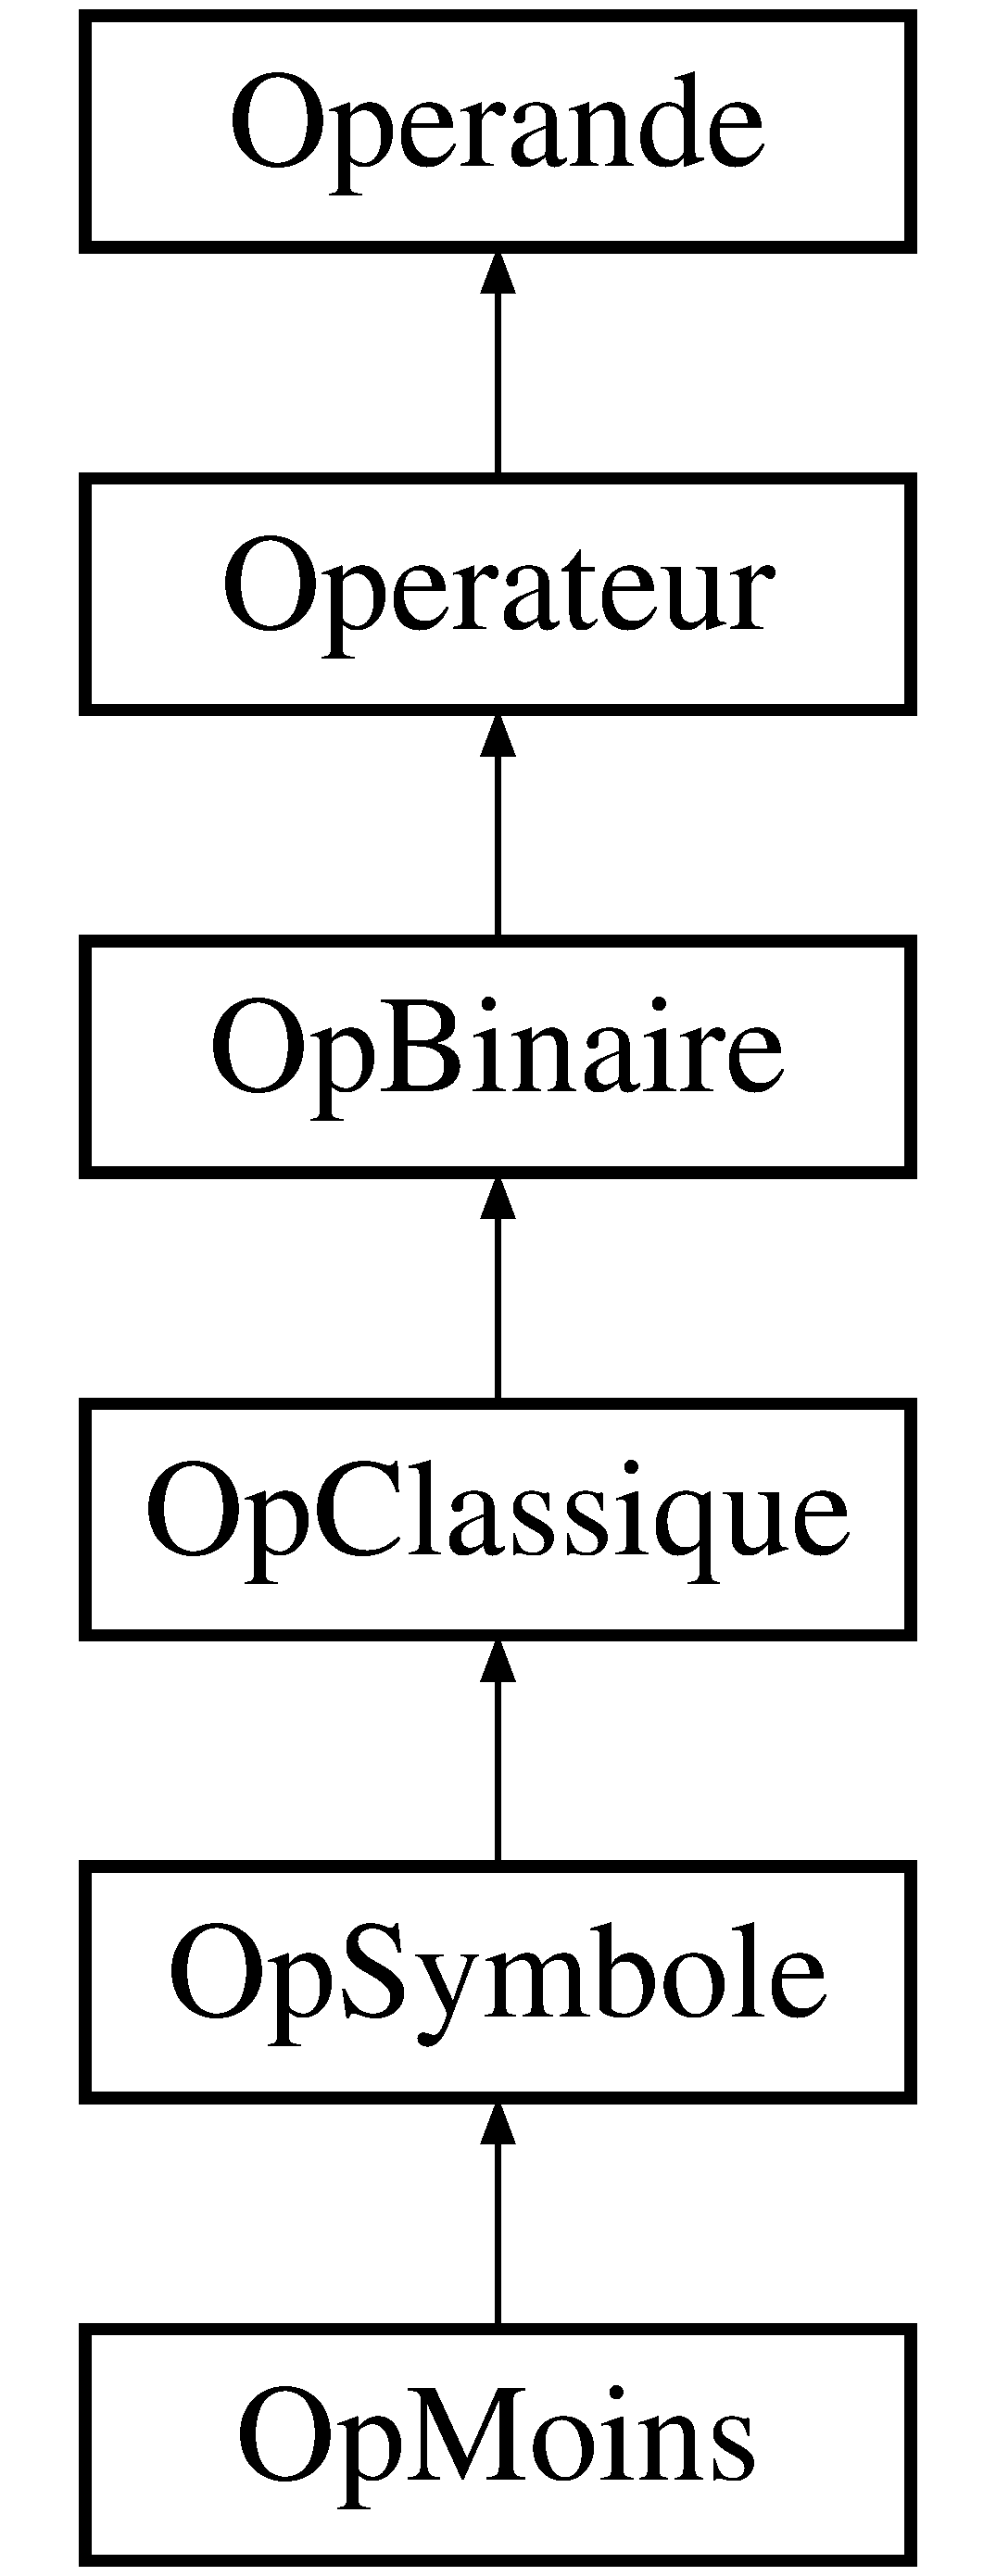
\includegraphics[height=6.000000cm]{class_op_moins}
\end{center}
\end{figure}
\subsection*{Public Member Functions}
\begin{DoxyCompactItemize}
\item 
\hyperlink{class_op_moins_a0220e5295f19be91875616b52d28453d}{Op\+Moins} ()
\item 
\hyperlink{class_litterale}{Litterale} $\ast$ \hyperlink{class_op_moins_a852637df56ddd5a98212559db77d0ed0}{action\+Num} (\hyperlink{class_entier}{Entier} \&arg1, \hyperlink{class_entier}{Entier} \&arg2)
\item 
\hyperlink{class_litterale}{Litterale} $\ast$ \hyperlink{class_op_moins_ab478b2dc55902bdad80ea811779d8466}{action\+Num} (\hyperlink{class_entier}{Entier} \&arg1, \hyperlink{class_reelle}{Reelle} \&arg2)
\item 
\hyperlink{class_litterale}{Litterale} $\ast$ \hyperlink{class_op_moins_a03336a72ebbbb55322ba4328affc56c6}{action\+Num} (\hyperlink{class_entier}{Entier} \&arg1, \hyperlink{class_rationnelle}{Rationnelle} \&arg2)
\item 
\hyperlink{class_litterale}{Litterale} $\ast$ \hyperlink{class_op_moins_a1673d5e6a39a07dc7ba20500de52067c}{action\+Num} (\hyperlink{class_reelle}{Reelle} \&arg1, \hyperlink{class_reelle}{Reelle} \&arg2)
\item 
\hyperlink{class_litterale}{Litterale} $\ast$ \hyperlink{class_op_moins_a0217de77568e1e5bab54af01f59d9e70}{action\+Num} (\hyperlink{class_reelle}{Reelle} \&arg1, \hyperlink{class_entier}{Entier} \&arg2)
\item 
\hyperlink{class_litterale}{Litterale} $\ast$ \hyperlink{class_op_moins_a6e72db9e3a3bf594e69c0c54513cb787}{action\+Num} (\hyperlink{class_reelle}{Reelle} \&arg1, \hyperlink{class_rationnelle}{Rationnelle} \&arg2)
\item 
\hyperlink{class_litterale}{Litterale} $\ast$ \hyperlink{class_op_moins_a75cd2784ee19446e28407e703487cdab}{action\+Num} (\hyperlink{class_rationnelle}{Rationnelle} \&arg1, \hyperlink{class_rationnelle}{Rationnelle} \&arg2)
\item 
\hyperlink{class_litterale}{Litterale} $\ast$ \hyperlink{class_op_moins_a6e87da6d4cd00822289d5d02e354fff3}{action\+Num} (\hyperlink{class_rationnelle}{Rationnelle} \&arg1, \hyperlink{class_entier}{Entier} \&arg2)
\item 
\hyperlink{class_litterale}{Litterale} $\ast$ \hyperlink{class_op_moins_af41b3759848a8293a9990be2b24bee6c}{action\+Num} (\hyperlink{class_rationnelle}{Rationnelle} \&arg1, \hyperlink{class_reelle}{Reelle} \&arg2)
\end{DoxyCompactItemize}
\subsection*{Additional Inherited Members}


\subsection{Detailed Description}


Definition at line 77 of file operator\+Classique.\+h.



\subsection{Constructor \& Destructor Documentation}
\index{Op\+Moins@{Op\+Moins}!Op\+Moins@{Op\+Moins}}
\index{Op\+Moins@{Op\+Moins}!Op\+Moins@{Op\+Moins}}
\subsubsection[{\texorpdfstring{Op\+Moins()}{OpMoins()}}]{\setlength{\rightskip}{0pt plus 5cm}Op\+Moins\+::\+Op\+Moins (
\begin{DoxyParamCaption}
{}
\end{DoxyParamCaption}
)\hspace{0.3cm}{\ttfamily [inline]}}\hypertarget{class_op_moins_a0220e5295f19be91875616b52d28453d}{}\label{class_op_moins_a0220e5295f19be91875616b52d28453d}


Definition at line 79 of file operator\+Classique.\+h.



\subsection{Member Function Documentation}
\index{Op\+Moins@{Op\+Moins}!action\+Num@{action\+Num}}
\index{action\+Num@{action\+Num}!Op\+Moins@{Op\+Moins}}
\subsubsection[{\texorpdfstring{action\+Num(\+Entier \&arg1, Entier \&arg2)}{actionNum(Entier &arg1, Entier &arg2)}}]{\setlength{\rightskip}{0pt plus 5cm}{\bf Litterale} $\ast$ Op\+Moins\+::action\+Num (
\begin{DoxyParamCaption}
\item[{{\bf Entier} \&}]{arg1, }
\item[{{\bf Entier} \&}]{arg2}
\end{DoxyParamCaption}
)\hspace{0.3cm}{\ttfamily [virtual]}}\hypertarget{class_op_moins_a852637df56ddd5a98212559db77d0ed0}{}\label{class_op_moins_a852637df56ddd5a98212559db77d0ed0}


Implements \hyperlink{class_op_symbole_a58c6b09cf3ccc1d753f6c5702eb3dfdd}{Op\+Symbole}.



Definition at line 177 of file operator\+Classique.\+cpp.

\index{Op\+Moins@{Op\+Moins}!action\+Num@{action\+Num}}
\index{action\+Num@{action\+Num}!Op\+Moins@{Op\+Moins}}
\subsubsection[{\texorpdfstring{action\+Num(\+Entier \&arg1, Reelle \&arg2)}{actionNum(Entier &arg1, Reelle &arg2)}}]{\setlength{\rightskip}{0pt plus 5cm}{\bf Litterale} $\ast$ Op\+Moins\+::action\+Num (
\begin{DoxyParamCaption}
\item[{{\bf Entier} \&}]{arg1, }
\item[{{\bf Reelle} \&}]{arg2}
\end{DoxyParamCaption}
)\hspace{0.3cm}{\ttfamily [virtual]}}\hypertarget{class_op_moins_ab478b2dc55902bdad80ea811779d8466}{}\label{class_op_moins_ab478b2dc55902bdad80ea811779d8466}


Implements \hyperlink{class_op_symbole_a99b426017e9db00066ca7f960b7ab5aa}{Op\+Symbole}.



Definition at line 186 of file operator\+Classique.\+cpp.

\index{Op\+Moins@{Op\+Moins}!action\+Num@{action\+Num}}
\index{action\+Num@{action\+Num}!Op\+Moins@{Op\+Moins}}
\subsubsection[{\texorpdfstring{action\+Num(\+Entier \&arg1, Rationnelle \&arg2)}{actionNum(Entier &arg1, Rationnelle &arg2)}}]{\setlength{\rightskip}{0pt plus 5cm}{\bf Litterale} $\ast$ Op\+Moins\+::action\+Num (
\begin{DoxyParamCaption}
\item[{{\bf Entier} \&}]{arg1, }
\item[{{\bf Rationnelle} \&}]{arg2}
\end{DoxyParamCaption}
)\hspace{0.3cm}{\ttfamily [virtual]}}\hypertarget{class_op_moins_a03336a72ebbbb55322ba4328affc56c6}{}\label{class_op_moins_a03336a72ebbbb55322ba4328affc56c6}


Implements \hyperlink{class_op_symbole_ae13989c55c53a7ec7c79d371ee05fbaa}{Op\+Symbole}.



Definition at line 195 of file operator\+Classique.\+cpp.

\index{Op\+Moins@{Op\+Moins}!action\+Num@{action\+Num}}
\index{action\+Num@{action\+Num}!Op\+Moins@{Op\+Moins}}
\subsubsection[{\texorpdfstring{action\+Num(\+Reelle \&arg1, Reelle \&arg2)}{actionNum(Reelle &arg1, Reelle &arg2)}}]{\setlength{\rightskip}{0pt plus 5cm}{\bf Litterale} $\ast$ Op\+Moins\+::action\+Num (
\begin{DoxyParamCaption}
\item[{{\bf Reelle} \&}]{arg1, }
\item[{{\bf Reelle} \&}]{arg2}
\end{DoxyParamCaption}
)\hspace{0.3cm}{\ttfamily [virtual]}}\hypertarget{class_op_moins_a1673d5e6a39a07dc7ba20500de52067c}{}\label{class_op_moins_a1673d5e6a39a07dc7ba20500de52067c}


Implements \hyperlink{class_op_symbole_a98cfb6ae979dbe1974aa03387c682634}{Op\+Symbole}.



Definition at line 210 of file operator\+Classique.\+cpp.

\index{Op\+Moins@{Op\+Moins}!action\+Num@{action\+Num}}
\index{action\+Num@{action\+Num}!Op\+Moins@{Op\+Moins}}
\subsubsection[{\texorpdfstring{action\+Num(\+Reelle \&arg1, Entier \&arg2)}{actionNum(Reelle &arg1, Entier &arg2)}}]{\setlength{\rightskip}{0pt plus 5cm}{\bf Litterale} $\ast$ Op\+Moins\+::action\+Num (
\begin{DoxyParamCaption}
\item[{{\bf Reelle} \&}]{arg1, }
\item[{{\bf Entier} \&}]{arg2}
\end{DoxyParamCaption}
)\hspace{0.3cm}{\ttfamily [virtual]}}\hypertarget{class_op_moins_a0217de77568e1e5bab54af01f59d9e70}{}\label{class_op_moins_a0217de77568e1e5bab54af01f59d9e70}


Implements \hyperlink{class_op_symbole_abfa9f422620f4fceaa18e5295b4c5b99}{Op\+Symbole}.



Definition at line 219 of file operator\+Classique.\+cpp.

\index{Op\+Moins@{Op\+Moins}!action\+Num@{action\+Num}}
\index{action\+Num@{action\+Num}!Op\+Moins@{Op\+Moins}}
\subsubsection[{\texorpdfstring{action\+Num(\+Reelle \&arg1, Rationnelle \&arg2)}{actionNum(Reelle &arg1, Rationnelle &arg2)}}]{\setlength{\rightskip}{0pt plus 5cm}{\bf Litterale} $\ast$ Op\+Moins\+::action\+Num (
\begin{DoxyParamCaption}
\item[{{\bf Reelle} \&}]{arg1, }
\item[{{\bf Rationnelle} \&}]{arg2}
\end{DoxyParamCaption}
)\hspace{0.3cm}{\ttfamily [virtual]}}\hypertarget{class_op_moins_a6e72db9e3a3bf594e69c0c54513cb787}{}\label{class_op_moins_a6e72db9e3a3bf594e69c0c54513cb787}


Implements \hyperlink{class_op_symbole_a184453513af4b3146e753520f1ee760f}{Op\+Symbole}.



Definition at line 228 of file operator\+Classique.\+cpp.

\index{Op\+Moins@{Op\+Moins}!action\+Num@{action\+Num}}
\index{action\+Num@{action\+Num}!Op\+Moins@{Op\+Moins}}
\subsubsection[{\texorpdfstring{action\+Num(\+Rationnelle \&arg1, Rationnelle \&arg2)}{actionNum(Rationnelle &arg1, Rationnelle &arg2)}}]{\setlength{\rightskip}{0pt plus 5cm}{\bf Litterale} $\ast$ Op\+Moins\+::action\+Num (
\begin{DoxyParamCaption}
\item[{{\bf Rationnelle} \&}]{arg1, }
\item[{{\bf Rationnelle} \&}]{arg2}
\end{DoxyParamCaption}
)\hspace{0.3cm}{\ttfamily [virtual]}}\hypertarget{class_op_moins_a75cd2784ee19446e28407e703487cdab}{}\label{class_op_moins_a75cd2784ee19446e28407e703487cdab}


Implements \hyperlink{class_op_symbole_ae63c8a614a14f75547919636e38c0901}{Op\+Symbole}.



Definition at line 238 of file operator\+Classique.\+cpp.

\index{Op\+Moins@{Op\+Moins}!action\+Num@{action\+Num}}
\index{action\+Num@{action\+Num}!Op\+Moins@{Op\+Moins}}
\subsubsection[{\texorpdfstring{action\+Num(\+Rationnelle \&arg1, Entier \&arg2)}{actionNum(Rationnelle &arg1, Entier &arg2)}}]{\setlength{\rightskip}{0pt plus 5cm}{\bf Litterale} $\ast$ Op\+Moins\+::action\+Num (
\begin{DoxyParamCaption}
\item[{{\bf Rationnelle} \&}]{arg1, }
\item[{{\bf Entier} \&}]{arg2}
\end{DoxyParamCaption}
)\hspace{0.3cm}{\ttfamily [virtual]}}\hypertarget{class_op_moins_a6e87da6d4cd00822289d5d02e354fff3}{}\label{class_op_moins_a6e87da6d4cd00822289d5d02e354fff3}


Implements \hyperlink{class_op_symbole_adcacf42cf2baf8d96c0997f28d546d8e}{Op\+Symbole}.



Definition at line 250 of file operator\+Classique.\+cpp.

\index{Op\+Moins@{Op\+Moins}!action\+Num@{action\+Num}}
\index{action\+Num@{action\+Num}!Op\+Moins@{Op\+Moins}}
\subsubsection[{\texorpdfstring{action\+Num(\+Rationnelle \&arg1, Reelle \&arg2)}{actionNum(Rationnelle &arg1, Reelle &arg2)}}]{\setlength{\rightskip}{0pt plus 5cm}{\bf Litterale} $\ast$ Op\+Moins\+::action\+Num (
\begin{DoxyParamCaption}
\item[{{\bf Rationnelle} \&}]{arg1, }
\item[{{\bf Reelle} \&}]{arg2}
\end{DoxyParamCaption}
)\hspace{0.3cm}{\ttfamily [virtual]}}\hypertarget{class_op_moins_af41b3759848a8293a9990be2b24bee6c}{}\label{class_op_moins_af41b3759848a8293a9990be2b24bee6c}


Implements \hyperlink{class_op_symbole_a031f540060b0744e7d2fa781a505e854}{Op\+Symbole}.



Definition at line 262 of file operator\+Classique.\+cpp.



The documentation for this class was generated from the following files\+:\begin{DoxyCompactItemize}
\item 
\hyperlink{operator_classique_8h}{operator\+Classique.\+h}\item 
\hyperlink{operator_classique_8cpp}{operator\+Classique.\+cpp}\end{DoxyCompactItemize}

\hypertarget{class_op_moins_factory}{}\section{Op\+Moins\+Factory Class Reference}
\label{class_op_moins_factory}\index{Op\+Moins\+Factory@{Op\+Moins\+Factory}}


{\ttfamily \#include $<$operator\+Factory.\+h$>$}

Inheritance diagram for Op\+Moins\+Factory\+:\begin{figure}[H]
\begin{center}
\leavevmode
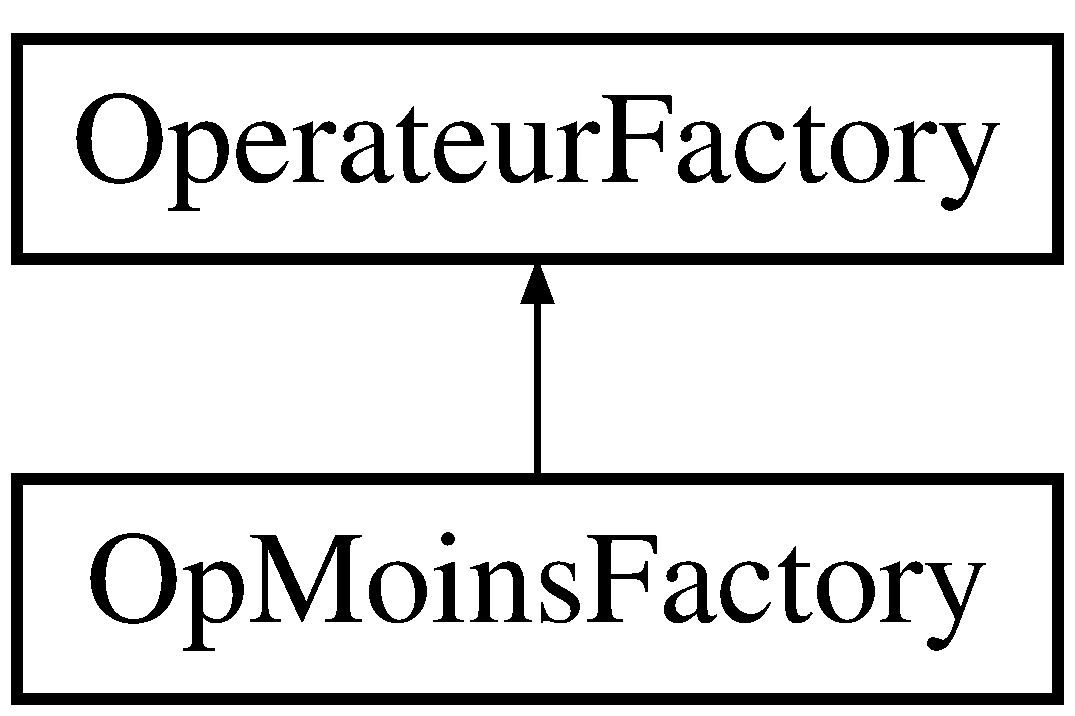
\includegraphics[height=2.000000cm]{class_op_moins_factory}
\end{center}
\end{figure}
\subsection*{Public Member Functions}
\begin{DoxyCompactItemize}
\item 
\hyperlink{class_op_moins_factory_aa769c2f1bebb49cfb2b32dcbbab22098}{Op\+Moins\+Factory} ()
\item 
\hyperlink{class_operateur}{Operateur} $\ast$ \hyperlink{class_op_moins_factory_a4caeb81946c415b7a547871c606c8888}{get\+Operateur} ()
\end{DoxyCompactItemize}
\subsection*{Additional Inherited Members}


\subsection{Detailed Description}


Definition at line 198 of file operator\+Factory.\+h.



\subsection{Constructor \& Destructor Documentation}
\index{Op\+Moins\+Factory@{Op\+Moins\+Factory}!Op\+Moins\+Factory@{Op\+Moins\+Factory}}
\index{Op\+Moins\+Factory@{Op\+Moins\+Factory}!Op\+Moins\+Factory@{Op\+Moins\+Factory}}
\subsubsection[{\texorpdfstring{Op\+Moins\+Factory()}{OpMoinsFactory()}}]{\setlength{\rightskip}{0pt plus 5cm}Op\+Moins\+Factory\+::\+Op\+Moins\+Factory (
\begin{DoxyParamCaption}
{}
\end{DoxyParamCaption}
)\hspace{0.3cm}{\ttfamily [inline]}}\hypertarget{class_op_moins_factory_aa769c2f1bebb49cfb2b32dcbbab22098}{}\label{class_op_moins_factory_aa769c2f1bebb49cfb2b32dcbbab22098}


Definition at line 200 of file operator\+Factory.\+h.



\subsection{Member Function Documentation}
\index{Op\+Moins\+Factory@{Op\+Moins\+Factory}!get\+Operateur@{get\+Operateur}}
\index{get\+Operateur@{get\+Operateur}!Op\+Moins\+Factory@{Op\+Moins\+Factory}}
\subsubsection[{\texorpdfstring{get\+Operateur()}{getOperateur()}}]{\setlength{\rightskip}{0pt plus 5cm}{\bf Operateur}$\ast$ Op\+Moins\+Factory\+::get\+Operateur (
\begin{DoxyParamCaption}
{}
\end{DoxyParamCaption}
)\hspace{0.3cm}{\ttfamily [inline]}, {\ttfamily [virtual]}}\hypertarget{class_op_moins_factory_a4caeb81946c415b7a547871c606c8888}{}\label{class_op_moins_factory_a4caeb81946c415b7a547871c606c8888}


Implements \hyperlink{class_operateur_factory_aff61b2f67451f086d6abaea4231b2d78}{Operateur\+Factory}.



Definition at line 201 of file operator\+Factory.\+h.



The documentation for this class was generated from the following file\+:\begin{DoxyCompactItemize}
\item 
\hyperlink{operator_factory_8h}{operator\+Factory.\+h}\end{DoxyCompactItemize}

\hypertarget{class_op_mul}{}\section{Op\+Mul Class Reference}
\label{class_op_mul}\index{Op\+Mul@{Op\+Mul}}


{\ttfamily \#include $<$operator\+Classique.\+h$>$}

Inheritance diagram for Op\+Mul\+:\begin{figure}[H]
\begin{center}
\leavevmode
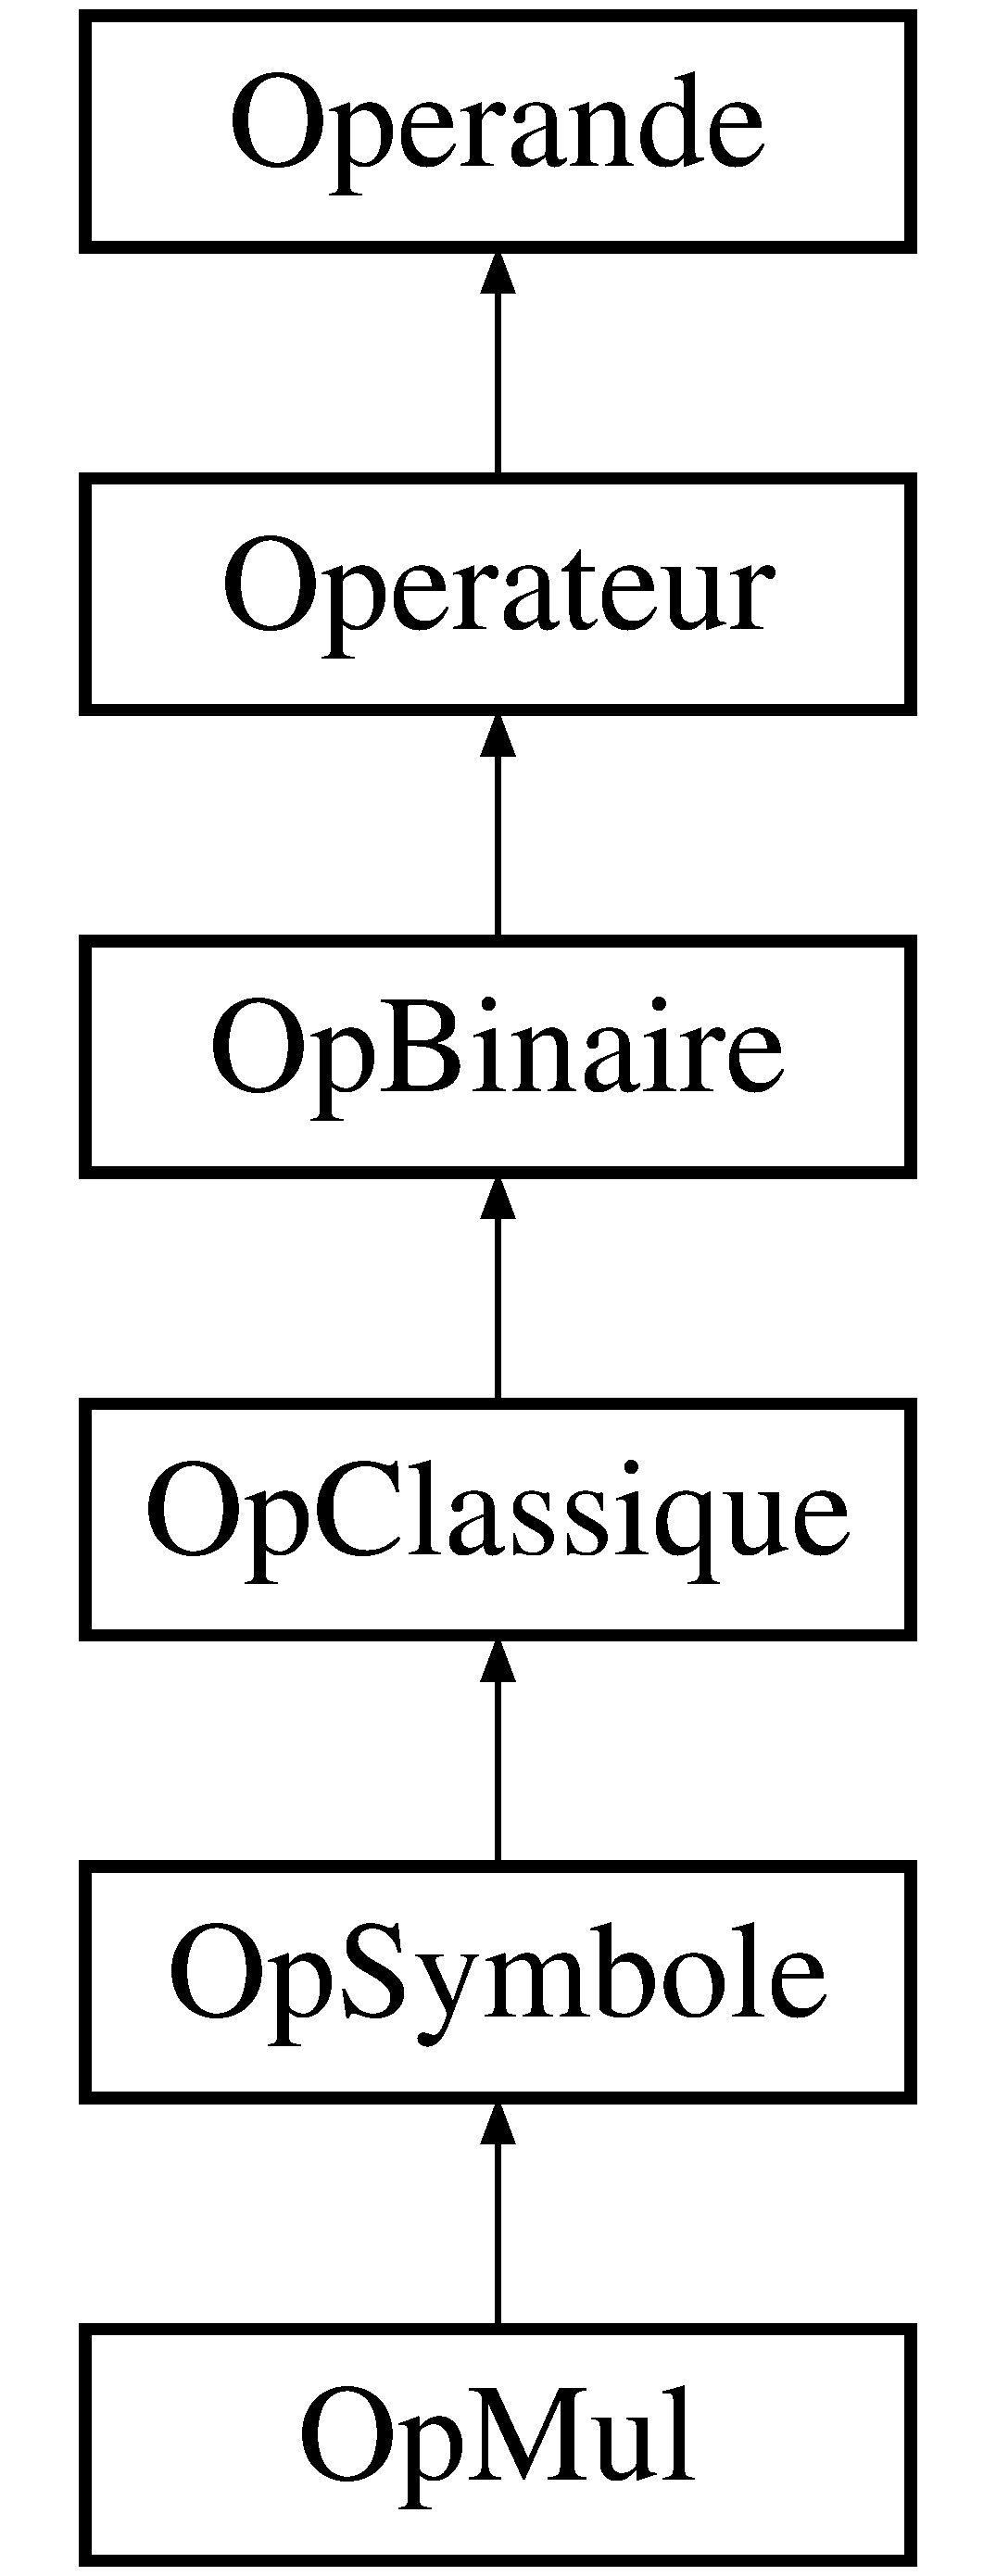
\includegraphics[height=6.000000cm]{class_op_mul}
\end{center}
\end{figure}
\subsection*{Public Member Functions}
\begin{DoxyCompactItemize}
\item 
\hyperlink{class_op_mul_a1269f54063d9f1966f935ed7f5340f82}{Op\+Mul} ()
\item 
\hyperlink{class_litterale}{Litterale} $\ast$ \hyperlink{class_op_mul_a92b4a0f259e3941c5dfb06baf0bb19eb}{fonction\+Num2} (\hyperlink{class_entier}{Entier} $\ast$arg1, \hyperlink{class_litterale}{Litterale} $\ast$arg2)
\item 
\hyperlink{class_litterale}{Litterale} $\ast$ \hyperlink{class_op_mul_a5334aed41233bfe0e32989a3162cb7f9}{fonction\+Num2} (\hyperlink{class_reelle}{Reelle} $\ast$arg1, \hyperlink{class_litterale}{Litterale} $\ast$arg2)
\item 
\hyperlink{class_litterale}{Litterale} $\ast$ \hyperlink{class_op_mul_a564ab9e0045bb0b9847d30271c62672c}{fonction\+Num2} (\hyperlink{class_rationnelle}{Rationnelle} $\ast$arg1, \hyperlink{class_litterale}{Litterale} $\ast$arg2)
\item 
\hyperlink{class_litterale}{Litterale} $\ast$ \hyperlink{class_op_mul_a583e93c4d996eacd3da73ccbcd5e4214}{action\+Num} (\hyperlink{class_entier}{Entier} \&arg1, \hyperlink{class_entier}{Entier} \&arg2)
\item 
\hyperlink{class_litterale}{Litterale} $\ast$ \hyperlink{class_op_mul_ae62bb21f5fbbaddaae0bea5aa3776ad4}{action\+Num} (\hyperlink{class_entier}{Entier} \&arg1, \hyperlink{class_reelle}{Reelle} \&arg2)
\item 
\hyperlink{class_litterale}{Litterale} $\ast$ \hyperlink{class_op_mul_ae0af76139e245c18a4b506de0e713dde}{action\+Num} (\hyperlink{class_entier}{Entier} \&arg1, \hyperlink{class_rationnelle}{Rationnelle} \&arg2)
\item 
\hyperlink{class_litterale}{Litterale} $\ast$ \hyperlink{class_op_mul_aa6a1c397cd419a0541f09da8581d01a3}{action\+Num} (\hyperlink{class_reelle}{Reelle} \&arg1, \hyperlink{class_reelle}{Reelle} \&arg2)
\item 
\hyperlink{class_litterale}{Litterale} $\ast$ \hyperlink{class_op_mul_a5f0374849c046a0744d8776bbda63a84}{action\+Num} (\hyperlink{class_reelle}{Reelle} \&arg1, \hyperlink{class_entier}{Entier} \&arg2)
\item 
\hyperlink{class_litterale}{Litterale} $\ast$ \hyperlink{class_op_mul_a8d5e27a1010461eeec33ae32546c8fbc}{action\+Num} (\hyperlink{class_reelle}{Reelle} \&arg1, \hyperlink{class_rationnelle}{Rationnelle} \&arg2)
\item 
\hyperlink{class_litterale}{Litterale} $\ast$ \hyperlink{class_op_mul_af6254f6a3aaeff62c6a05d1aa6f2d91e}{action\+Num} (\hyperlink{class_rationnelle}{Rationnelle} \&arg1, \hyperlink{class_rationnelle}{Rationnelle} \&arg2)
\item 
\hyperlink{class_litterale}{Litterale} $\ast$ \hyperlink{class_op_mul_a11ff74a40a9da95e7b44e2a7a995424f}{action\+Num} (\hyperlink{class_rationnelle}{Rationnelle} \&arg1, \hyperlink{class_entier}{Entier} \&arg2)
\item 
\hyperlink{class_litterale}{Litterale} $\ast$ \hyperlink{class_op_mul_ad8431cde5f0f7ee09f0f5e76c7bd489c}{action\+Num} (\hyperlink{class_rationnelle}{Rationnelle} \&arg1, \hyperlink{class_reelle}{Reelle} \&arg2)
\end{DoxyCompactItemize}
\subsection*{Additional Inherited Members}


\subsection{Detailed Description}


Definition at line 109 of file operator\+Classique.\+h.



\subsection{Constructor \& Destructor Documentation}
\index{Op\+Mul@{Op\+Mul}!Op\+Mul@{Op\+Mul}}
\index{Op\+Mul@{Op\+Mul}!Op\+Mul@{Op\+Mul}}
\subsubsection[{\texorpdfstring{Op\+Mul()}{OpMul()}}]{\setlength{\rightskip}{0pt plus 5cm}Op\+Mul\+::\+Op\+Mul (
\begin{DoxyParamCaption}
{}
\end{DoxyParamCaption}
)\hspace{0.3cm}{\ttfamily [inline]}}\hypertarget{class_op_mul_a1269f54063d9f1966f935ed7f5340f82}{}\label{class_op_mul_a1269f54063d9f1966f935ed7f5340f82}


Definition at line 111 of file operator\+Classique.\+h.



\subsection{Member Function Documentation}
\index{Op\+Mul@{Op\+Mul}!action\+Num@{action\+Num}}
\index{action\+Num@{action\+Num}!Op\+Mul@{Op\+Mul}}
\subsubsection[{\texorpdfstring{action\+Num(\+Entier \&arg1, Entier \&arg2)}{actionNum(Entier &arg1, Entier &arg2)}}]{\setlength{\rightskip}{0pt plus 5cm}{\bf Litterale} $\ast$ Op\+Mul\+::action\+Num (
\begin{DoxyParamCaption}
\item[{{\bf Entier} \&}]{arg1, }
\item[{{\bf Entier} \&}]{arg2}
\end{DoxyParamCaption}
)\hspace{0.3cm}{\ttfamily [virtual]}}\hypertarget{class_op_mul_a583e93c4d996eacd3da73ccbcd5e4214}{}\label{class_op_mul_a583e93c4d996eacd3da73ccbcd5e4214}


Implements \hyperlink{class_op_symbole_a58c6b09cf3ccc1d753f6c5702eb3dfdd}{Op\+Symbole}.



Definition at line 370 of file operator\+Classique.\+cpp.

\index{Op\+Mul@{Op\+Mul}!action\+Num@{action\+Num}}
\index{action\+Num@{action\+Num}!Op\+Mul@{Op\+Mul}}
\subsubsection[{\texorpdfstring{action\+Num(\+Entier \&arg1, Reelle \&arg2)}{actionNum(Entier &arg1, Reelle &arg2)}}]{\setlength{\rightskip}{0pt plus 5cm}{\bf Litterale} $\ast$ Op\+Mul\+::action\+Num (
\begin{DoxyParamCaption}
\item[{{\bf Entier} \&}]{arg1, }
\item[{{\bf Reelle} \&}]{arg2}
\end{DoxyParamCaption}
)\hspace{0.3cm}{\ttfamily [virtual]}}\hypertarget{class_op_mul_ae62bb21f5fbbaddaae0bea5aa3776ad4}{}\label{class_op_mul_ae62bb21f5fbbaddaae0bea5aa3776ad4}


Implements \hyperlink{class_op_symbole_a99b426017e9db00066ca7f960b7ab5aa}{Op\+Symbole}.



Definition at line 373 of file operator\+Classique.\+cpp.

\index{Op\+Mul@{Op\+Mul}!action\+Num@{action\+Num}}
\index{action\+Num@{action\+Num}!Op\+Mul@{Op\+Mul}}
\subsubsection[{\texorpdfstring{action\+Num(\+Entier \&arg1, Rationnelle \&arg2)}{actionNum(Entier &arg1, Rationnelle &arg2)}}]{\setlength{\rightskip}{0pt plus 5cm}{\bf Litterale} $\ast$ Op\+Mul\+::action\+Num (
\begin{DoxyParamCaption}
\item[{{\bf Entier} \&}]{arg1, }
\item[{{\bf Rationnelle} \&}]{arg2}
\end{DoxyParamCaption}
)\hspace{0.3cm}{\ttfamily [virtual]}}\hypertarget{class_op_mul_ae0af76139e245c18a4b506de0e713dde}{}\label{class_op_mul_ae0af76139e245c18a4b506de0e713dde}


Implements \hyperlink{class_op_symbole_ae13989c55c53a7ec7c79d371ee05fbaa}{Op\+Symbole}.



Definition at line 376 of file operator\+Classique.\+cpp.

\index{Op\+Mul@{Op\+Mul}!action\+Num@{action\+Num}}
\index{action\+Num@{action\+Num}!Op\+Mul@{Op\+Mul}}
\subsubsection[{\texorpdfstring{action\+Num(\+Reelle \&arg1, Reelle \&arg2)}{actionNum(Reelle &arg1, Reelle &arg2)}}]{\setlength{\rightskip}{0pt plus 5cm}{\bf Litterale} $\ast$ Op\+Mul\+::action\+Num (
\begin{DoxyParamCaption}
\item[{{\bf Reelle} \&}]{arg1, }
\item[{{\bf Reelle} \&}]{arg2}
\end{DoxyParamCaption}
)\hspace{0.3cm}{\ttfamily [virtual]}}\hypertarget{class_op_mul_aa6a1c397cd419a0541f09da8581d01a3}{}\label{class_op_mul_aa6a1c397cd419a0541f09da8581d01a3}


Implements \hyperlink{class_op_symbole_a98cfb6ae979dbe1974aa03387c682634}{Op\+Symbole}.



Definition at line 381 of file operator\+Classique.\+cpp.

\index{Op\+Mul@{Op\+Mul}!action\+Num@{action\+Num}}
\index{action\+Num@{action\+Num}!Op\+Mul@{Op\+Mul}}
\subsubsection[{\texorpdfstring{action\+Num(\+Reelle \&arg1, Entier \&arg2)}{actionNum(Reelle &arg1, Entier &arg2)}}]{\setlength{\rightskip}{0pt plus 5cm}{\bf Litterale} $\ast$ Op\+Mul\+::action\+Num (
\begin{DoxyParamCaption}
\item[{{\bf Reelle} \&}]{arg1, }
\item[{{\bf Entier} \&}]{arg2}
\end{DoxyParamCaption}
)\hspace{0.3cm}{\ttfamily [virtual]}}\hypertarget{class_op_mul_a5f0374849c046a0744d8776bbda63a84}{}\label{class_op_mul_a5f0374849c046a0744d8776bbda63a84}


Implements \hyperlink{class_op_symbole_abfa9f422620f4fceaa18e5295b4c5b99}{Op\+Symbole}.



Definition at line 384 of file operator\+Classique.\+cpp.

\index{Op\+Mul@{Op\+Mul}!action\+Num@{action\+Num}}
\index{action\+Num@{action\+Num}!Op\+Mul@{Op\+Mul}}
\subsubsection[{\texorpdfstring{action\+Num(\+Reelle \&arg1, Rationnelle \&arg2)}{actionNum(Reelle &arg1, Rationnelle &arg2)}}]{\setlength{\rightskip}{0pt plus 5cm}{\bf Litterale} $\ast$ Op\+Mul\+::action\+Num (
\begin{DoxyParamCaption}
\item[{{\bf Reelle} \&}]{arg1, }
\item[{{\bf Rationnelle} \&}]{arg2}
\end{DoxyParamCaption}
)\hspace{0.3cm}{\ttfamily [virtual]}}\hypertarget{class_op_mul_a8d5e27a1010461eeec33ae32546c8fbc}{}\label{class_op_mul_a8d5e27a1010461eeec33ae32546c8fbc}


Implements \hyperlink{class_op_symbole_a184453513af4b3146e753520f1ee760f}{Op\+Symbole}.



Definition at line 387 of file operator\+Classique.\+cpp.

\index{Op\+Mul@{Op\+Mul}!action\+Num@{action\+Num}}
\index{action\+Num@{action\+Num}!Op\+Mul@{Op\+Mul}}
\subsubsection[{\texorpdfstring{action\+Num(\+Rationnelle \&arg1, Rationnelle \&arg2)}{actionNum(Rationnelle &arg1, Rationnelle &arg2)}}]{\setlength{\rightskip}{0pt plus 5cm}{\bf Litterale} $\ast$ Op\+Mul\+::action\+Num (
\begin{DoxyParamCaption}
\item[{{\bf Rationnelle} \&}]{arg1, }
\item[{{\bf Rationnelle} \&}]{arg2}
\end{DoxyParamCaption}
)\hspace{0.3cm}{\ttfamily [virtual]}}\hypertarget{class_op_mul_af6254f6a3aaeff62c6a05d1aa6f2d91e}{}\label{class_op_mul_af6254f6a3aaeff62c6a05d1aa6f2d91e}


Implements \hyperlink{class_op_symbole_ae63c8a614a14f75547919636e38c0901}{Op\+Symbole}.



Definition at line 391 of file operator\+Classique.\+cpp.

\index{Op\+Mul@{Op\+Mul}!action\+Num@{action\+Num}}
\index{action\+Num@{action\+Num}!Op\+Mul@{Op\+Mul}}
\subsubsection[{\texorpdfstring{action\+Num(\+Rationnelle \&arg1, Entier \&arg2)}{actionNum(Rationnelle &arg1, Entier &arg2)}}]{\setlength{\rightskip}{0pt plus 5cm}{\bf Litterale} $\ast$ Op\+Mul\+::action\+Num (
\begin{DoxyParamCaption}
\item[{{\bf Rationnelle} \&}]{arg1, }
\item[{{\bf Entier} \&}]{arg2}
\end{DoxyParamCaption}
)\hspace{0.3cm}{\ttfamily [virtual]}}\hypertarget{class_op_mul_a11ff74a40a9da95e7b44e2a7a995424f}{}\label{class_op_mul_a11ff74a40a9da95e7b44e2a7a995424f}


Implements \hyperlink{class_op_symbole_adcacf42cf2baf8d96c0997f28d546d8e}{Op\+Symbole}.



Definition at line 396 of file operator\+Classique.\+cpp.

\index{Op\+Mul@{Op\+Mul}!action\+Num@{action\+Num}}
\index{action\+Num@{action\+Num}!Op\+Mul@{Op\+Mul}}
\subsubsection[{\texorpdfstring{action\+Num(\+Rationnelle \&arg1, Reelle \&arg2)}{actionNum(Rationnelle &arg1, Reelle &arg2)}}]{\setlength{\rightskip}{0pt plus 5cm}{\bf Litterale} $\ast$ Op\+Mul\+::action\+Num (
\begin{DoxyParamCaption}
\item[{{\bf Rationnelle} \&}]{arg1, }
\item[{{\bf Reelle} \&}]{arg2}
\end{DoxyParamCaption}
)\hspace{0.3cm}{\ttfamily [virtual]}}\hypertarget{class_op_mul_ad8431cde5f0f7ee09f0f5e76c7bd489c}{}\label{class_op_mul_ad8431cde5f0f7ee09f0f5e76c7bd489c}


Implements \hyperlink{class_op_symbole_a031f540060b0744e7d2fa781a505e854}{Op\+Symbole}.



Definition at line 401 of file operator\+Classique.\+cpp.

\index{Op\+Mul@{Op\+Mul}!fonction\+Num2@{fonction\+Num2}}
\index{fonction\+Num2@{fonction\+Num2}!Op\+Mul@{Op\+Mul}}
\subsubsection[{\texorpdfstring{fonction\+Num2(\+Entier $\ast$arg1, Litterale $\ast$arg2)}{fonctionNum2(Entier *arg1, Litterale *arg2)}}]{\setlength{\rightskip}{0pt plus 5cm}{\bf Litterale} $\ast$ Op\+Mul\+::fonction\+Num2 (
\begin{DoxyParamCaption}
\item[{{\bf Entier} $\ast$}]{arg1, }
\item[{{\bf Litterale} $\ast$}]{arg2}
\end{DoxyParamCaption}
)\hspace{0.3cm}{\ttfamily [virtual]}}\hypertarget{class_op_mul_a92b4a0f259e3941c5dfb06baf0bb19eb}{}\label{class_op_mul_a92b4a0f259e3941c5dfb06baf0bb19eb}


Reimplemented from \hyperlink{class_op_symbole_a69e1f5709d9ffba309d094856252eca7}{Op\+Symbole}.



Definition at line 342 of file operator\+Classique.\+cpp.

\index{Op\+Mul@{Op\+Mul}!fonction\+Num2@{fonction\+Num2}}
\index{fonction\+Num2@{fonction\+Num2}!Op\+Mul@{Op\+Mul}}
\subsubsection[{\texorpdfstring{fonction\+Num2(\+Reelle $\ast$arg1, Litterale $\ast$arg2)}{fonctionNum2(Reelle *arg1, Litterale *arg2)}}]{\setlength{\rightskip}{0pt plus 5cm}{\bf Litterale} $\ast$ Op\+Mul\+::fonction\+Num2 (
\begin{DoxyParamCaption}
\item[{{\bf Reelle} $\ast$}]{arg1, }
\item[{{\bf Litterale} $\ast$}]{arg2}
\end{DoxyParamCaption}
)\hspace{0.3cm}{\ttfamily [virtual]}}\hypertarget{class_op_mul_a5334aed41233bfe0e32989a3162cb7f9}{}\label{class_op_mul_a5334aed41233bfe0e32989a3162cb7f9}


Reimplemented from \hyperlink{class_op_symbole_adacb4ef49ad6f19403a12b91ecb0c0f1}{Op\+Symbole}.



Definition at line 351 of file operator\+Classique.\+cpp.

\index{Op\+Mul@{Op\+Mul}!fonction\+Num2@{fonction\+Num2}}
\index{fonction\+Num2@{fonction\+Num2}!Op\+Mul@{Op\+Mul}}
\subsubsection[{\texorpdfstring{fonction\+Num2(\+Rationnelle $\ast$arg1, Litterale $\ast$arg2)}{fonctionNum2(Rationnelle *arg1, Litterale *arg2)}}]{\setlength{\rightskip}{0pt plus 5cm}{\bf Litterale} $\ast$ Op\+Mul\+::fonction\+Num2 (
\begin{DoxyParamCaption}
\item[{{\bf Rationnelle} $\ast$}]{arg1, }
\item[{{\bf Litterale} $\ast$}]{arg2}
\end{DoxyParamCaption}
)\hspace{0.3cm}{\ttfamily [virtual]}}\hypertarget{class_op_mul_a564ab9e0045bb0b9847d30271c62672c}{}\label{class_op_mul_a564ab9e0045bb0b9847d30271c62672c}


Reimplemented from \hyperlink{class_op_symbole_a20ab54596cc3f3c8cdd059e13dc51541}{Op\+Symbole}.



Definition at line 360 of file operator\+Classique.\+cpp.



The documentation for this class was generated from the following files\+:\begin{DoxyCompactItemize}
\item 
\hyperlink{operator_classique_8h}{operator\+Classique.\+h}\item 
\hyperlink{operator_classique_8cpp}{operator\+Classique.\+cpp}\end{DoxyCompactItemize}

\hypertarget{class_op_mul_factory}{}\section{Op\+Mul\+Factory Class Reference}
\label{class_op_mul_factory}\index{Op\+Mul\+Factory@{Op\+Mul\+Factory}}


{\ttfamily \#include $<$operator\+Factory.\+h$>$}

Inheritance diagram for Op\+Mul\+Factory\+:\begin{figure}[H]
\begin{center}
\leavevmode
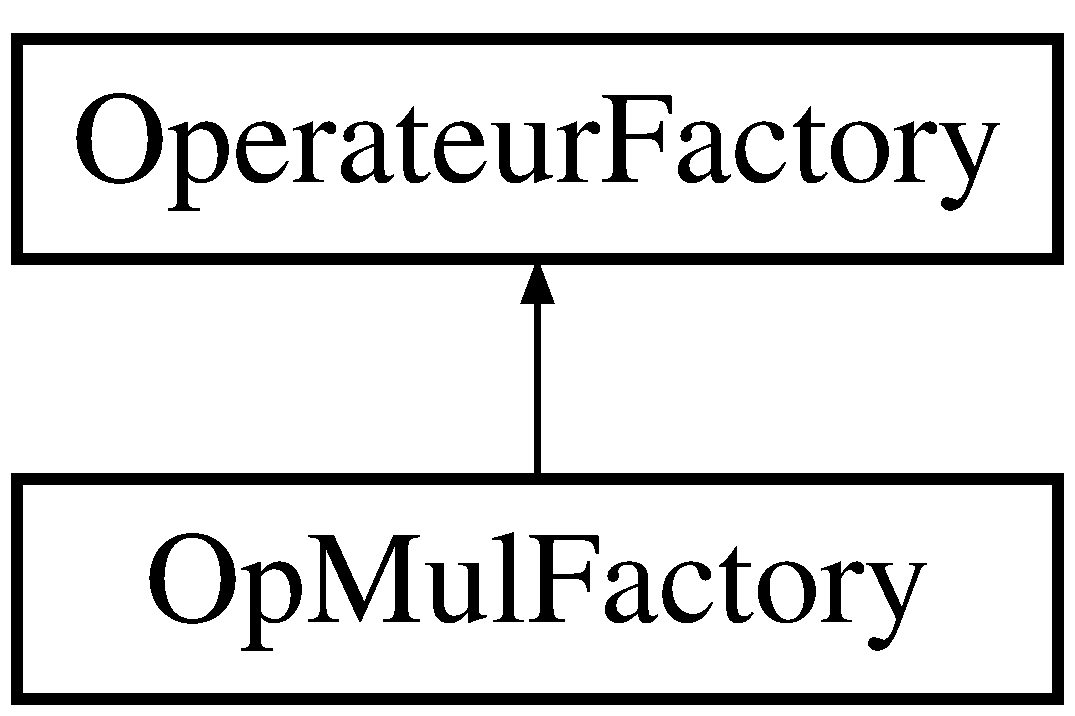
\includegraphics[height=2.000000cm]{class_op_mul_factory}
\end{center}
\end{figure}
\subsection*{Public Member Functions}
\begin{DoxyCompactItemize}
\item 
\hyperlink{class_op_mul_factory_a98202ba00822ed25c87a48c4bf18664c}{Op\+Mul\+Factory} ()
\item 
\hyperlink{class_operateur}{Operateur} $\ast$ \hyperlink{class_op_mul_factory_a05fcb523c96c05b6b86d83b56cd49038}{get\+Operateur} ()
\end{DoxyCompactItemize}
\subsection*{Additional Inherited Members}


\subsection{Detailed Description}


Definition at line 204 of file operator\+Factory.\+h.



\subsection{Constructor \& Destructor Documentation}
\index{Op\+Mul\+Factory@{Op\+Mul\+Factory}!Op\+Mul\+Factory@{Op\+Mul\+Factory}}
\index{Op\+Mul\+Factory@{Op\+Mul\+Factory}!Op\+Mul\+Factory@{Op\+Mul\+Factory}}
\subsubsection[{\texorpdfstring{Op\+Mul\+Factory()}{OpMulFactory()}}]{\setlength{\rightskip}{0pt plus 5cm}Op\+Mul\+Factory\+::\+Op\+Mul\+Factory (
\begin{DoxyParamCaption}
{}
\end{DoxyParamCaption}
)\hspace{0.3cm}{\ttfamily [inline]}}\hypertarget{class_op_mul_factory_a98202ba00822ed25c87a48c4bf18664c}{}\label{class_op_mul_factory_a98202ba00822ed25c87a48c4bf18664c}


Definition at line 206 of file operator\+Factory.\+h.



\subsection{Member Function Documentation}
\index{Op\+Mul\+Factory@{Op\+Mul\+Factory}!get\+Operateur@{get\+Operateur}}
\index{get\+Operateur@{get\+Operateur}!Op\+Mul\+Factory@{Op\+Mul\+Factory}}
\subsubsection[{\texorpdfstring{get\+Operateur()}{getOperateur()}}]{\setlength{\rightskip}{0pt plus 5cm}{\bf Operateur}$\ast$ Op\+Mul\+Factory\+::get\+Operateur (
\begin{DoxyParamCaption}
{}
\end{DoxyParamCaption}
)\hspace{0.3cm}{\ttfamily [inline]}, {\ttfamily [virtual]}}\hypertarget{class_op_mul_factory_a05fcb523c96c05b6b86d83b56cd49038}{}\label{class_op_mul_factory_a05fcb523c96c05b6b86d83b56cd49038}


Implements \hyperlink{class_operateur_factory_aff61b2f67451f086d6abaea4231b2d78}{Operateur\+Factory}.



Definition at line 207 of file operator\+Factory.\+h.



The documentation for this class was generated from the following file\+:\begin{DoxyCompactItemize}
\item 
\hyperlink{operator_factory_8h}{operator\+Factory.\+h}\end{DoxyCompactItemize}

\hypertarget{class_op_neg}{}\section{Op\+Neg Class Reference}
\label{class_op_neg}\index{Op\+Neg@{Op\+Neg}}


{\ttfamily \#include $<$operator.\+h$>$}

Inheritance diagram for Op\+Neg\+:\begin{figure}[H]
\begin{center}
\leavevmode
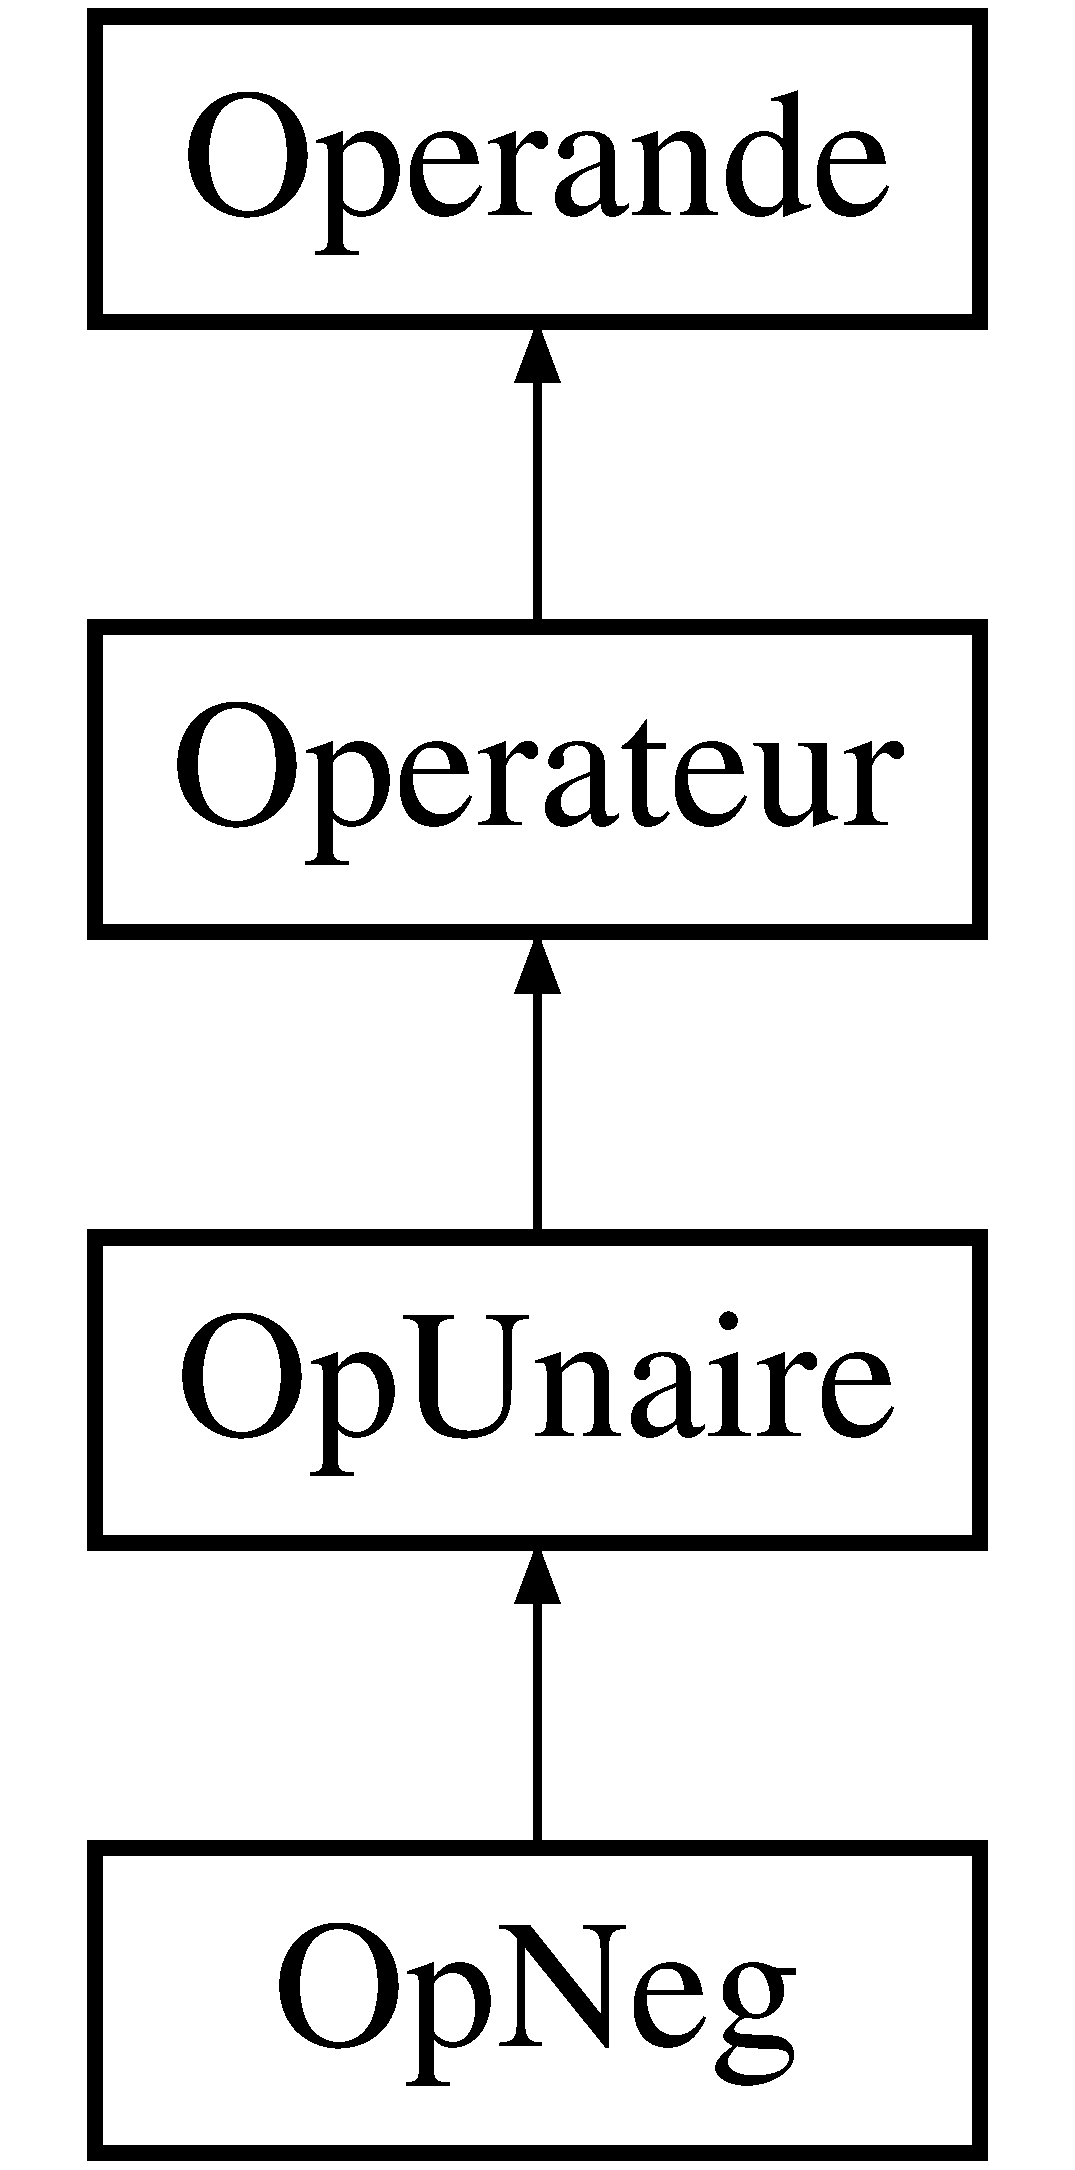
\includegraphics[height=4.000000cm]{class_op_neg}
\end{center}
\end{figure}
\subsection*{Public Member Functions}
\begin{DoxyCompactItemize}
\item 
\hyperlink{class_op_neg_a61eb1bf7e525d382980b913da91515aa}{Op\+Neg} ()
\item 
\hyperlink{class_litterale}{Litterale} $\ast$ \hyperlink{class_op_neg_aba05bfb2ea8d1061303c2f98201b42c1}{fonction\+Num} (\hyperlink{class_nombres}{Nombres} $\ast$arg1)
\item 
\hyperlink{class_litterale}{Litterale} $\ast$ \hyperlink{class_op_neg_a716a9d79a42c5d5993bcc7bab10a167e}{action\+Num} (\hyperlink{class_entier}{Entier} \&arg1)
\item 
\hyperlink{class_litterale}{Litterale} $\ast$ \hyperlink{class_op_neg_a18050dc2d64ca60845616b295af9b10c}{action\+Num} (\hyperlink{class_reelle}{Reelle} \&arg1)
\item 
\hyperlink{class_litterale}{Litterale} $\ast$ \hyperlink{class_op_neg_a8801e50e3b9af195d71c3324b2aa4c33}{action\+Num} (\hyperlink{class_rationnelle}{Rationnelle} \&arg1)
\end{DoxyCompactItemize}
\subsection*{Additional Inherited Members}


\subsection{Detailed Description}


Definition at line 127 of file operator.\+h.



\subsection{Constructor \& Destructor Documentation}
\index{Op\+Neg@{Op\+Neg}!Op\+Neg@{Op\+Neg}}
\index{Op\+Neg@{Op\+Neg}!Op\+Neg@{Op\+Neg}}
\subsubsection[{\texorpdfstring{Op\+Neg()}{OpNeg()}}]{\setlength{\rightskip}{0pt plus 5cm}Op\+Neg\+::\+Op\+Neg (
\begin{DoxyParamCaption}
{}
\end{DoxyParamCaption}
)\hspace{0.3cm}{\ttfamily [inline]}}\hypertarget{class_op_neg_a61eb1bf7e525d382980b913da91515aa}{}\label{class_op_neg_a61eb1bf7e525d382980b913da91515aa}


Definition at line 129 of file operator.\+h.



\subsection{Member Function Documentation}
\index{Op\+Neg@{Op\+Neg}!action\+Num@{action\+Num}}
\index{action\+Num@{action\+Num}!Op\+Neg@{Op\+Neg}}
\subsubsection[{\texorpdfstring{action\+Num(\+Entier \&arg1)}{actionNum(Entier &arg1)}}]{\setlength{\rightskip}{0pt plus 5cm}{\bf Litterale} $\ast$ Op\+Neg\+::action\+Num (
\begin{DoxyParamCaption}
\item[{{\bf Entier} \&}]{arg1}
\end{DoxyParamCaption}
)\hspace{0.3cm}{\ttfamily [virtual]}}\hypertarget{class_op_neg_a716a9d79a42c5d5993bcc7bab10a167e}{}\label{class_op_neg_a716a9d79a42c5d5993bcc7bab10a167e}


Implements \hyperlink{class_op_unaire_a4db1c0cbd6ec4acbe89a6ef2ae68f901}{Op\+Unaire}.



Definition at line 70 of file operator.\+cpp.

\index{Op\+Neg@{Op\+Neg}!action\+Num@{action\+Num}}
\index{action\+Num@{action\+Num}!Op\+Neg@{Op\+Neg}}
\subsubsection[{\texorpdfstring{action\+Num(\+Reelle \&arg1)}{actionNum(Reelle &arg1)}}]{\setlength{\rightskip}{0pt plus 5cm}{\bf Litterale} $\ast$ Op\+Neg\+::action\+Num (
\begin{DoxyParamCaption}
\item[{{\bf Reelle} \&}]{arg1}
\end{DoxyParamCaption}
)\hspace{0.3cm}{\ttfamily [virtual]}}\hypertarget{class_op_neg_a18050dc2d64ca60845616b295af9b10c}{}\label{class_op_neg_a18050dc2d64ca60845616b295af9b10c}


Implements \hyperlink{class_op_unaire_a0b92d632cf248e765783f23d6d637d1f}{Op\+Unaire}.



Definition at line 74 of file operator.\+cpp.

\index{Op\+Neg@{Op\+Neg}!action\+Num@{action\+Num}}
\index{action\+Num@{action\+Num}!Op\+Neg@{Op\+Neg}}
\subsubsection[{\texorpdfstring{action\+Num(\+Rationnelle \&arg1)}{actionNum(Rationnelle &arg1)}}]{\setlength{\rightskip}{0pt plus 5cm}{\bf Litterale} $\ast$ Op\+Neg\+::action\+Num (
\begin{DoxyParamCaption}
\item[{{\bf Rationnelle} \&}]{arg1}
\end{DoxyParamCaption}
)\hspace{0.3cm}{\ttfamily [virtual]}}\hypertarget{class_op_neg_a8801e50e3b9af195d71c3324b2aa4c33}{}\label{class_op_neg_a8801e50e3b9af195d71c3324b2aa4c33}


Implements \hyperlink{class_op_unaire_a7728e3d41bfe8ace1f9343a4cd404502}{Op\+Unaire}.



Definition at line 79 of file operator.\+cpp.

\index{Op\+Neg@{Op\+Neg}!fonction\+Num@{fonction\+Num}}
\index{fonction\+Num@{fonction\+Num}!Op\+Neg@{Op\+Neg}}
\subsubsection[{\texorpdfstring{fonction\+Num(\+Nombres $\ast$arg1)}{fonctionNum(Nombres *arg1)}}]{\setlength{\rightskip}{0pt plus 5cm}{\bf Litterale} $\ast$ Op\+Neg\+::fonction\+Num (
\begin{DoxyParamCaption}
\item[{{\bf Nombres} $\ast$}]{arg1}
\end{DoxyParamCaption}
)\hspace{0.3cm}{\ttfamily [virtual]}}\hypertarget{class_op_neg_aba05bfb2ea8d1061303c2f98201b42c1}{}\label{class_op_neg_aba05bfb2ea8d1061303c2f98201b42c1}


Reimplemented from \hyperlink{class_op_unaire_a05586cb26efdcc8fa3aba5be681a71c8}{Op\+Unaire}.



Definition at line 66 of file operator.\+cpp.



The documentation for this class was generated from the following files\+:\begin{DoxyCompactItemize}
\item 
\hyperlink{operator_8h}{operator.\+h}\item 
\hyperlink{operator_8cpp}{operator.\+cpp}\end{DoxyCompactItemize}

\hypertarget{class_op_neg_factory}{}\section{Op\+Neg\+Factory Class Reference}
\label{class_op_neg_factory}\index{Op\+Neg\+Factory@{Op\+Neg\+Factory}}


{\ttfamily \#include $<$operator\+Factory.\+h$>$}

Inheritance diagram for Op\+Neg\+Factory\+:\begin{figure}[H]
\begin{center}
\leavevmode
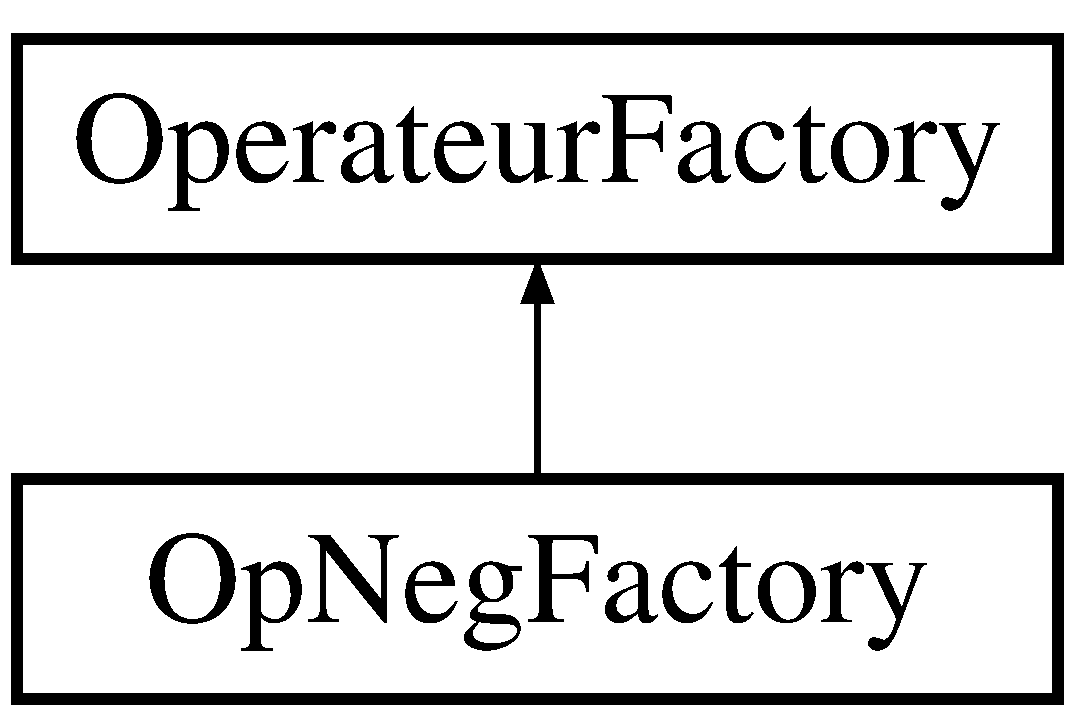
\includegraphics[height=2.000000cm]{class_op_neg_factory}
\end{center}
\end{figure}
\subsection*{Public Member Functions}
\begin{DoxyCompactItemize}
\item 
\hyperlink{class_op_neg_factory_afa8b4f4e292e7b4eb281b5f7ff9c2c2a}{Op\+Neg\+Factory} ()
\item 
\hyperlink{class_operateur}{Operateur} $\ast$ \hyperlink{class_op_neg_factory_a7f6cc922bb250ba8da46bfb26bd4acdc}{get\+Operateur} ()
\end{DoxyCompactItemize}
\subsection*{Additional Inherited Members}


\subsection{Detailed Description}


Definition at line 75 of file operator\+Factory.\+h.



\subsection{Constructor \& Destructor Documentation}
\index{Op\+Neg\+Factory@{Op\+Neg\+Factory}!Op\+Neg\+Factory@{Op\+Neg\+Factory}}
\index{Op\+Neg\+Factory@{Op\+Neg\+Factory}!Op\+Neg\+Factory@{Op\+Neg\+Factory}}
\subsubsection[{\texorpdfstring{Op\+Neg\+Factory()}{OpNegFactory()}}]{\setlength{\rightskip}{0pt plus 5cm}Op\+Neg\+Factory\+::\+Op\+Neg\+Factory (
\begin{DoxyParamCaption}
{}
\end{DoxyParamCaption}
)\hspace{0.3cm}{\ttfamily [inline]}}\hypertarget{class_op_neg_factory_afa8b4f4e292e7b4eb281b5f7ff9c2c2a}{}\label{class_op_neg_factory_afa8b4f4e292e7b4eb281b5f7ff9c2c2a}


Definition at line 77 of file operator\+Factory.\+h.



\subsection{Member Function Documentation}
\index{Op\+Neg\+Factory@{Op\+Neg\+Factory}!get\+Operateur@{get\+Operateur}}
\index{get\+Operateur@{get\+Operateur}!Op\+Neg\+Factory@{Op\+Neg\+Factory}}
\subsubsection[{\texorpdfstring{get\+Operateur()}{getOperateur()}}]{\setlength{\rightskip}{0pt plus 5cm}{\bf Operateur}$\ast$ Op\+Neg\+Factory\+::get\+Operateur (
\begin{DoxyParamCaption}
{}
\end{DoxyParamCaption}
)\hspace{0.3cm}{\ttfamily [inline]}, {\ttfamily [virtual]}}\hypertarget{class_op_neg_factory_a7f6cc922bb250ba8da46bfb26bd4acdc}{}\label{class_op_neg_factory_a7f6cc922bb250ba8da46bfb26bd4acdc}


Implements \hyperlink{class_operateur_factory_aff61b2f67451f086d6abaea4231b2d78}{Operateur\+Factory}.



Definition at line 78 of file operator\+Factory.\+h.



The documentation for this class was generated from the following file\+:\begin{DoxyCompactItemize}
\item 
\hyperlink{operator_factory_8h}{operator\+Factory.\+h}\end{DoxyCompactItemize}

\hypertarget{class_op_not}{}\section{Op\+Not Class Reference}
\label{class_op_not}\index{Op\+Not@{Op\+Not}}


{\ttfamily \#include $<$operator.\+h$>$}

Inheritance diagram for Op\+Not\+:\begin{figure}[H]
\begin{center}
\leavevmode
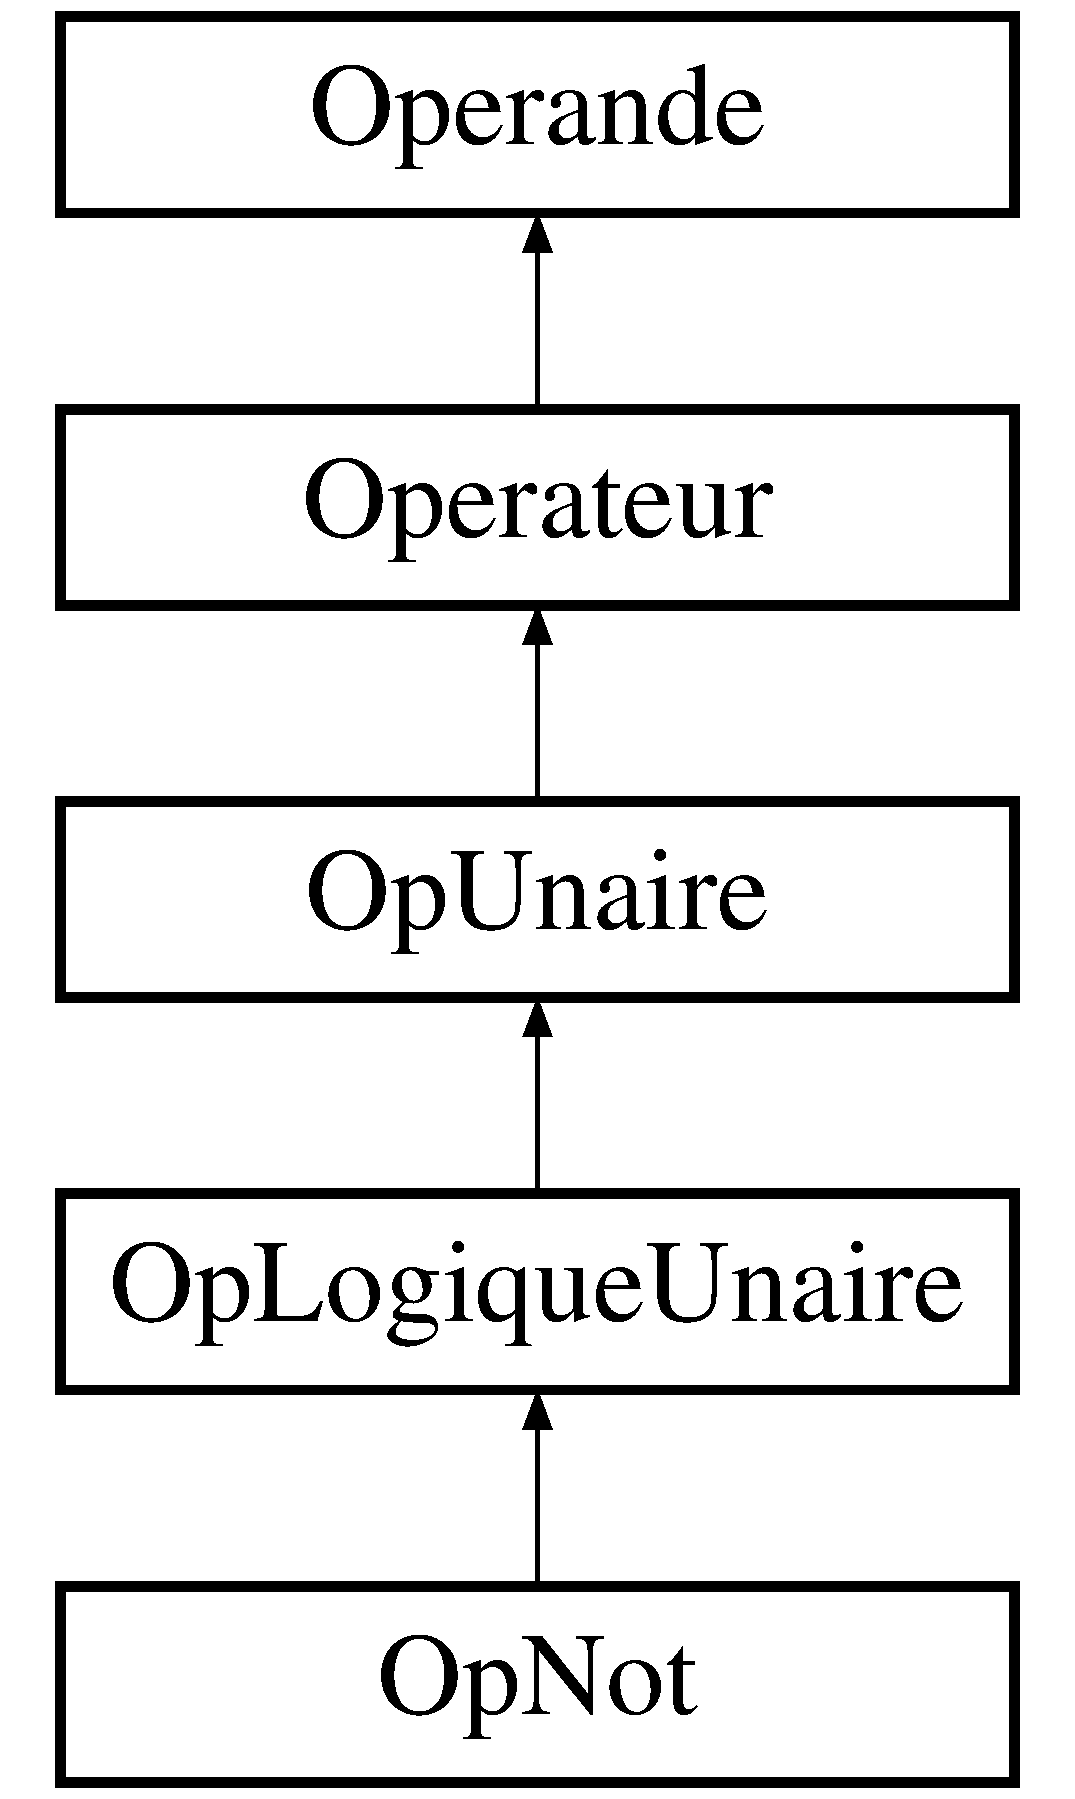
\includegraphics[height=5.000000cm]{class_op_not}
\end{center}
\end{figure}
\subsection*{Public Member Functions}
\begin{DoxyCompactItemize}
\item 
\hyperlink{class_op_not_acf1ca13f4f9016b74f912f3d68c9ad29}{Op\+Not} ()
\item 
\hyperlink{class_litterale}{Litterale} $\ast$ \hyperlink{class_op_not_ad4a6fdf0a1de9ee9d41d87db5e872604}{action\+Logi\+Numerique} (\hyperlink{class_lit_numerique}{Lit\+Numerique} $\ast$arg1)
\end{DoxyCompactItemize}
\subsection*{Additional Inherited Members}


\subsection{Detailed Description}


Definition at line 57 of file operator.\+h.



\subsection{Constructor \& Destructor Documentation}
\index{Op\+Not@{Op\+Not}!Op\+Not@{Op\+Not}}
\index{Op\+Not@{Op\+Not}!Op\+Not@{Op\+Not}}
\subsubsection[{\texorpdfstring{Op\+Not()}{OpNot()}}]{\setlength{\rightskip}{0pt plus 5cm}Op\+Not\+::\+Op\+Not (
\begin{DoxyParamCaption}
{}
\end{DoxyParamCaption}
)\hspace{0.3cm}{\ttfamily [inline]}}\hypertarget{class_op_not_acf1ca13f4f9016b74f912f3d68c9ad29}{}\label{class_op_not_acf1ca13f4f9016b74f912f3d68c9ad29}


Definition at line 59 of file operator.\+h.



\subsection{Member Function Documentation}
\index{Op\+Not@{Op\+Not}!action\+Logi\+Numerique@{action\+Logi\+Numerique}}
\index{action\+Logi\+Numerique@{action\+Logi\+Numerique}!Op\+Not@{Op\+Not}}
\subsubsection[{\texorpdfstring{action\+Logi\+Numerique(\+Lit\+Numerique $\ast$arg1)}{actionLogiNumerique(LitNumerique *arg1)}}]{\setlength{\rightskip}{0pt plus 5cm}{\bf Litterale} $\ast$ Op\+Not\+::action\+Logi\+Numerique (
\begin{DoxyParamCaption}
\item[{{\bf Lit\+Numerique} $\ast$}]{arg1}
\end{DoxyParamCaption}
)\hspace{0.3cm}{\ttfamily [virtual]}}\hypertarget{class_op_not_ad4a6fdf0a1de9ee9d41d87db5e872604}{}\label{class_op_not_ad4a6fdf0a1de9ee9d41d87db5e872604}


Implements \hyperlink{class_op_logique_unaire_a89c5a27b3dc232cf69aa1631231c3fc6}{Op\+Logique\+Unaire}.



Definition at line 201 of file operator.\+cpp.



The documentation for this class was generated from the following files\+:\begin{DoxyCompactItemize}
\item 
\hyperlink{operator_8h}{operator.\+h}\item 
\hyperlink{operator_8cpp}{operator.\+cpp}\end{DoxyCompactItemize}

\hypertarget{class_op_not_factory}{}\section{Op\+Not\+Factory Class Reference}
\label{class_op_not_factory}\index{Op\+Not\+Factory@{Op\+Not\+Factory}}


{\ttfamily \#include $<$operator\+Factory.\+h$>$}

Inheritance diagram for Op\+Not\+Factory\+:\begin{figure}[H]
\begin{center}
\leavevmode
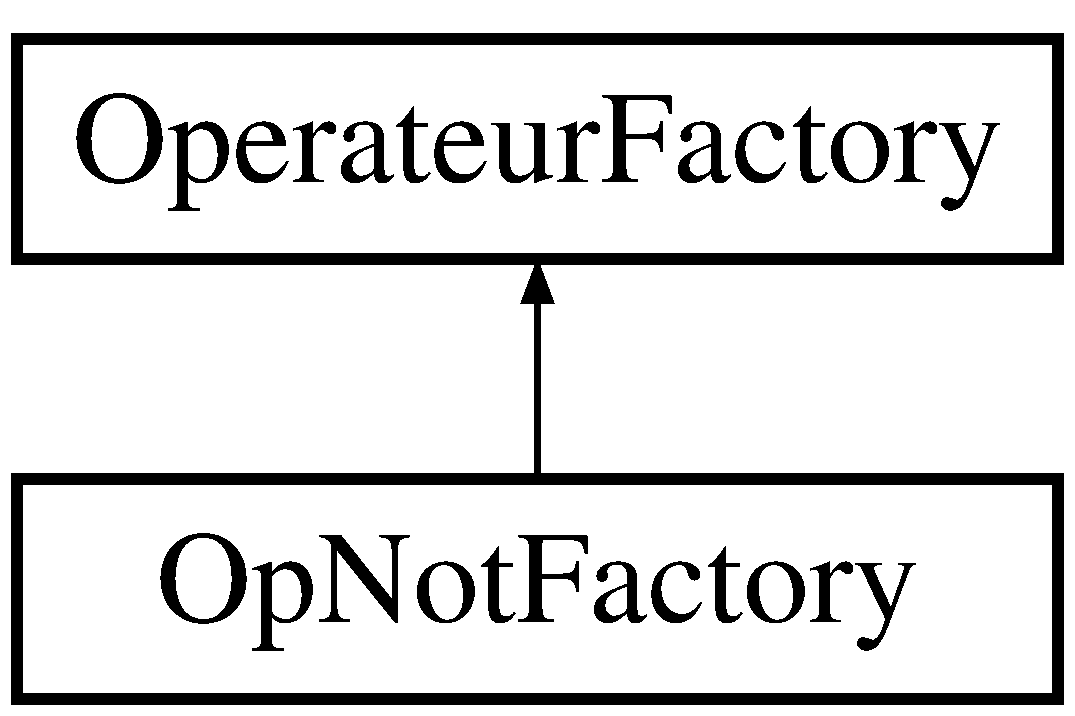
\includegraphics[height=2.000000cm]{class_op_not_factory}
\end{center}
\end{figure}
\subsection*{Public Member Functions}
\begin{DoxyCompactItemize}
\item 
\hyperlink{class_op_not_factory_a4d23167b825d67f4d12c05cc1ac367ec}{Op\+Not\+Factory} ()
\item 
\hyperlink{class_operateur}{Operateur} $\ast$ \hyperlink{class_op_not_factory_a375472ef36be910af8d81983e9237ca7}{get\+Operateur} ()
\end{DoxyCompactItemize}
\subsection*{Additional Inherited Members}


\subsection{Detailed Description}


Definition at line 185 of file operator\+Factory.\+h.



\subsection{Constructor \& Destructor Documentation}
\index{Op\+Not\+Factory@{Op\+Not\+Factory}!Op\+Not\+Factory@{Op\+Not\+Factory}}
\index{Op\+Not\+Factory@{Op\+Not\+Factory}!Op\+Not\+Factory@{Op\+Not\+Factory}}
\subsubsection[{\texorpdfstring{Op\+Not\+Factory()}{OpNotFactory()}}]{\setlength{\rightskip}{0pt plus 5cm}Op\+Not\+Factory\+::\+Op\+Not\+Factory (
\begin{DoxyParamCaption}
{}
\end{DoxyParamCaption}
)\hspace{0.3cm}{\ttfamily [inline]}}\hypertarget{class_op_not_factory_a4d23167b825d67f4d12c05cc1ac367ec}{}\label{class_op_not_factory_a4d23167b825d67f4d12c05cc1ac367ec}


Definition at line 187 of file operator\+Factory.\+h.



\subsection{Member Function Documentation}
\index{Op\+Not\+Factory@{Op\+Not\+Factory}!get\+Operateur@{get\+Operateur}}
\index{get\+Operateur@{get\+Operateur}!Op\+Not\+Factory@{Op\+Not\+Factory}}
\subsubsection[{\texorpdfstring{get\+Operateur()}{getOperateur()}}]{\setlength{\rightskip}{0pt plus 5cm}{\bf Operateur}$\ast$ Op\+Not\+Factory\+::get\+Operateur (
\begin{DoxyParamCaption}
{}
\end{DoxyParamCaption}
)\hspace{0.3cm}{\ttfamily [inline]}, {\ttfamily [virtual]}}\hypertarget{class_op_not_factory_a375472ef36be910af8d81983e9237ca7}{}\label{class_op_not_factory_a375472ef36be910af8d81983e9237ca7}


Implements \hyperlink{class_operateur_factory_aff61b2f67451f086d6abaea4231b2d78}{Operateur\+Factory}.



Definition at line 188 of file operator\+Factory.\+h.



The documentation for this class was generated from the following file\+:\begin{DoxyCompactItemize}
\item 
\hyperlink{operator_factory_8h}{operator\+Factory.\+h}\end{DoxyCompactItemize}

\hypertarget{class_op_or}{}\section{Op\+Or Class Reference}
\label{class_op_or}\index{Op\+Or@{Op\+Or}}


{\ttfamily \#include $<$operator\+Logique.\+h$>$}

Inheritance diagram for Op\+Or\+:\begin{figure}[H]
\begin{center}
\leavevmode
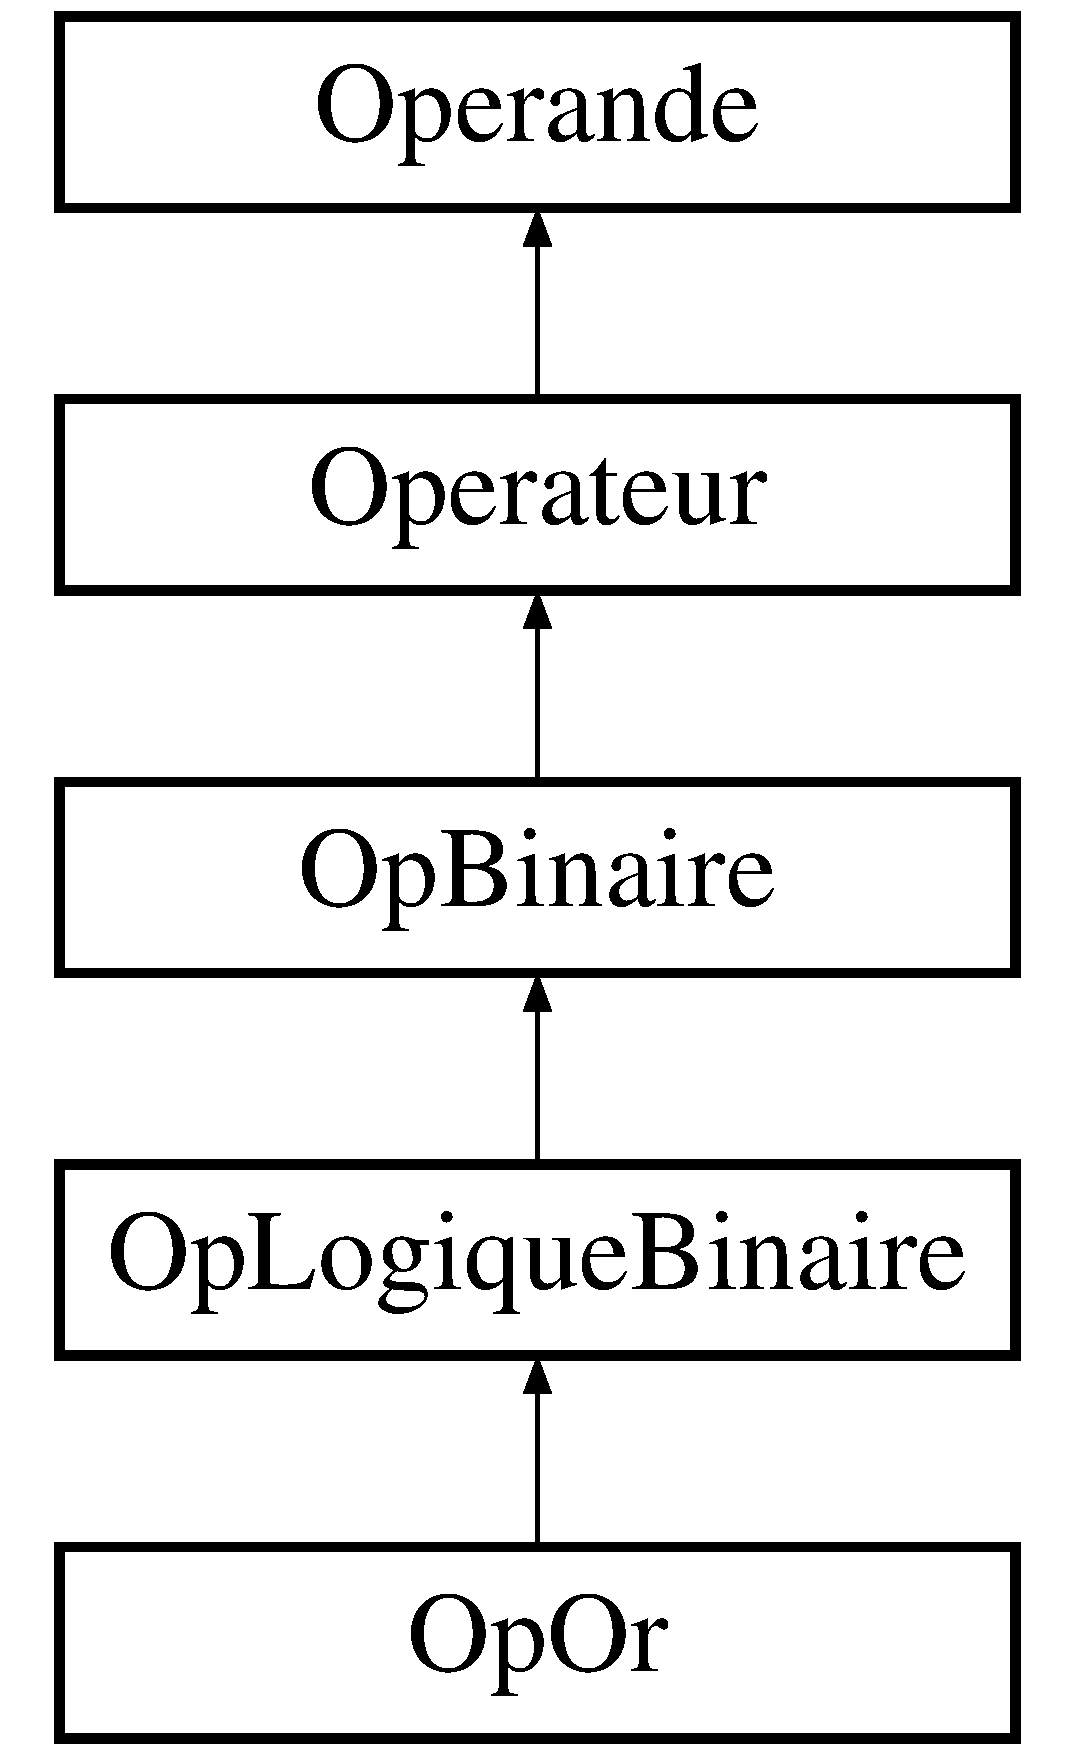
\includegraphics[height=5.000000cm]{class_op_or}
\end{center}
\end{figure}
\subsection*{Public Member Functions}
\begin{DoxyCompactItemize}
\item 
\hyperlink{class_op_or_ad85888dd43eab7621258d3a4a4a2c4e9}{Op\+Or} ()
\item 
\hyperlink{class_litterale}{Litterale} $\ast$ \hyperlink{class_op_or_ad2fe1c5e10d965fb3292bb2b41ba1a70}{action\+Logi\+Numerique} (\hyperlink{class_lit_numerique}{Lit\+Numerique} $\ast$arg1, \hyperlink{class_lit_numerique}{Lit\+Numerique} $\ast$arg2)
\end{DoxyCompactItemize}
\subsection*{Additional Inherited Members}


\subsection{Detailed Description}


Definition at line 68 of file operator\+Logique.\+h.



\subsection{Constructor \& Destructor Documentation}
\index{Op\+Or@{Op\+Or}!Op\+Or@{Op\+Or}}
\index{Op\+Or@{Op\+Or}!Op\+Or@{Op\+Or}}
\subsubsection[{\texorpdfstring{Op\+Or()}{OpOr()}}]{\setlength{\rightskip}{0pt plus 5cm}Op\+Or\+::\+Op\+Or (
\begin{DoxyParamCaption}
{}
\end{DoxyParamCaption}
)\hspace{0.3cm}{\ttfamily [inline]}}\hypertarget{class_op_or_ad85888dd43eab7621258d3a4a4a2c4e9}{}\label{class_op_or_ad85888dd43eab7621258d3a4a4a2c4e9}


Definition at line 70 of file operator\+Logique.\+h.



\subsection{Member Function Documentation}
\index{Op\+Or@{Op\+Or}!action\+Logi\+Numerique@{action\+Logi\+Numerique}}
\index{action\+Logi\+Numerique@{action\+Logi\+Numerique}!Op\+Or@{Op\+Or}}
\subsubsection[{\texorpdfstring{action\+Logi\+Numerique(\+Lit\+Numerique $\ast$arg1, Lit\+Numerique $\ast$arg2)}{actionLogiNumerique(LitNumerique *arg1, LitNumerique *arg2)}}]{\setlength{\rightskip}{0pt plus 5cm}{\bf Litterale} $\ast$ Op\+Or\+::action\+Logi\+Numerique (
\begin{DoxyParamCaption}
\item[{{\bf Lit\+Numerique} $\ast$}]{arg1, }
\item[{{\bf Lit\+Numerique} $\ast$}]{arg2}
\end{DoxyParamCaption}
)\hspace{0.3cm}{\ttfamily [virtual]}}\hypertarget{class_op_or_ad2fe1c5e10d965fb3292bb2b41ba1a70}{}\label{class_op_or_ad2fe1c5e10d965fb3292bb2b41ba1a70}


Implements \hyperlink{class_op_logique_binaire_a8fcab4c45ebcadbbcfecfa0c02e36f21}{Op\+Logique\+Binaire}.



Definition at line 60 of file operator\+Logique.\+cpp.



The documentation for this class was generated from the following files\+:\begin{DoxyCompactItemize}
\item 
\hyperlink{operator_logique_8h}{operator\+Logique.\+h}\item 
\hyperlink{operator_logique_8cpp}{operator\+Logique.\+cpp}\end{DoxyCompactItemize}

\hypertarget{class_op_or_factory}{}\section{Op\+Or\+Factory Class Reference}
\label{class_op_or_factory}\index{Op\+Or\+Factory@{Op\+Or\+Factory}}


{\ttfamily \#include $<$operator\+Factory.\+h$>$}

Inheritance diagram for Op\+Or\+Factory\+:\begin{figure}[H]
\begin{center}
\leavevmode
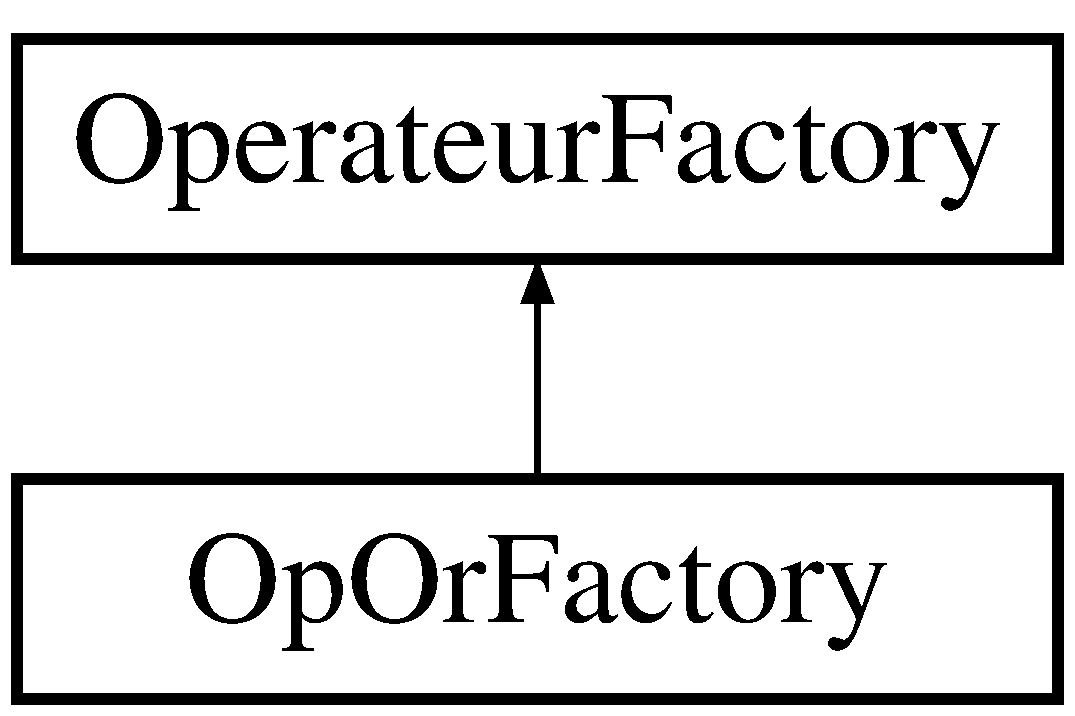
\includegraphics[height=2.000000cm]{class_op_or_factory}
\end{center}
\end{figure}
\subsection*{Public Member Functions}
\begin{DoxyCompactItemize}
\item 
\hyperlink{class_op_or_factory_a61e366473f9a753f6c7b11f05d8dcaa0}{Op\+Or\+Factory} ()
\item 
\hyperlink{class_operateur}{Operateur} $\ast$ \hyperlink{class_op_or_factory_a6b703fc7860b9ceda4f33c7820081f9b}{get\+Operateur} ()
\end{DoxyCompactItemize}
\subsection*{Additional Inherited Members}


\subsection{Detailed Description}


Definition at line 179 of file operator\+Factory.\+h.



\subsection{Constructor \& Destructor Documentation}
\index{Op\+Or\+Factory@{Op\+Or\+Factory}!Op\+Or\+Factory@{Op\+Or\+Factory}}
\index{Op\+Or\+Factory@{Op\+Or\+Factory}!Op\+Or\+Factory@{Op\+Or\+Factory}}
\subsubsection[{\texorpdfstring{Op\+Or\+Factory()}{OpOrFactory()}}]{\setlength{\rightskip}{0pt plus 5cm}Op\+Or\+Factory\+::\+Op\+Or\+Factory (
\begin{DoxyParamCaption}
{}
\end{DoxyParamCaption}
)\hspace{0.3cm}{\ttfamily [inline]}}\hypertarget{class_op_or_factory_a61e366473f9a753f6c7b11f05d8dcaa0}{}\label{class_op_or_factory_a61e366473f9a753f6c7b11f05d8dcaa0}


Definition at line 181 of file operator\+Factory.\+h.



\subsection{Member Function Documentation}
\index{Op\+Or\+Factory@{Op\+Or\+Factory}!get\+Operateur@{get\+Operateur}}
\index{get\+Operateur@{get\+Operateur}!Op\+Or\+Factory@{Op\+Or\+Factory}}
\subsubsection[{\texorpdfstring{get\+Operateur()}{getOperateur()}}]{\setlength{\rightskip}{0pt plus 5cm}{\bf Operateur}$\ast$ Op\+Or\+Factory\+::get\+Operateur (
\begin{DoxyParamCaption}
{}
\end{DoxyParamCaption}
)\hspace{0.3cm}{\ttfamily [inline]}, {\ttfamily [virtual]}}\hypertarget{class_op_or_factory_a6b703fc7860b9ceda4f33c7820081f9b}{}\label{class_op_or_factory_a6b703fc7860b9ceda4f33c7820081f9b}


Implements \hyperlink{class_operateur_factory_aff61b2f67451f086d6abaea4231b2d78}{Operateur\+Factory}.



Definition at line 182 of file operator\+Factory.\+h.



The documentation for this class was generated from the following file\+:\begin{DoxyCompactItemize}
\item 
\hyperlink{operator_factory_8h}{operator\+Factory.\+h}\end{DoxyCompactItemize}

\hypertarget{class_op_pile}{}\section{Op\+Pile Class Reference}
\label{class_op_pile}\index{Op\+Pile@{Op\+Pile}}


{\ttfamily \#include $<$operator.\+h$>$}

Inheritance diagram for Op\+Pile\+:\begin{figure}[H]
\begin{center}
\leavevmode
\includegraphics[height=5.000000cm]{class_op_pile}
\end{center}
\end{figure}
\subsection*{Public Member Functions}
\begin{DoxyCompactItemize}
\item 
\hyperlink{class_op_pile_abeb5537a96ae74f0a5e1fdfb4da0dd92}{Op\+Pile} (const Q\+String \&na, unsigned int size)
\item 
virtual \hyperlink{class_op_pile_aaae1a74325c449101411ab6b30715c59}{$\sim$\+Op\+Pile} ()
\item 
void \hyperlink{class_op_pile_ac05c50b3c226d57dbb866442ab8fd5e3}{add\+Arg} (\hyperlink{class_pile}{Pile} $\ast$pile)
\item 
\hyperlink{class_litterale}{Litterale} $\ast$ \hyperlink{class_op_pile_a02b47fa3b5f7399a09681c80353024e0}{executer} ()
\item 
virtual void \hyperlink{class_op_pile_a57de213f1b5281de1c37b83ecd8b0cd7}{executer\+Pile} ()=0
\item 
void \hyperlink{class_op_pile_ac67eb5ad0445529cfee741b1f71b0851}{set\+Pile} (\hyperlink{class_pile}{Pile} $\ast$p1)
\end{DoxyCompactItemize}
\subsection*{Protected Attributes}
\begin{DoxyCompactItemize}
\item 
\hyperlink{class_pile}{Pile} $\ast$ \hyperlink{class_op_pile_a702ec066d54bdb84b9980a1343c7f5f4}{lit\+Aff}
\end{DoxyCompactItemize}


\subsection{Detailed Description}


Definition at line 203 of file operator.\+h.



\subsection{Constructor \& Destructor Documentation}
\index{Op\+Pile@{Op\+Pile}!Op\+Pile@{Op\+Pile}}
\index{Op\+Pile@{Op\+Pile}!Op\+Pile@{Op\+Pile}}
\subsubsection[{\texorpdfstring{Op\+Pile(const Q\+String \&na, unsigned int size)}{OpPile(const QString &na, unsigned int size)}}]{\setlength{\rightskip}{0pt plus 5cm}Op\+Pile\+::\+Op\+Pile (
\begin{DoxyParamCaption}
\item[{const Q\+String \&}]{na, }
\item[{unsigned int}]{size}
\end{DoxyParamCaption}
)\hspace{0.3cm}{\ttfamily [inline]}}\hypertarget{class_op_pile_abeb5537a96ae74f0a5e1fdfb4da0dd92}{}\label{class_op_pile_abeb5537a96ae74f0a5e1fdfb4da0dd92}


Definition at line 207 of file operator.\+h.

\index{Op\+Pile@{Op\+Pile}!````~Op\+Pile@{$\sim$\+Op\+Pile}}
\index{````~Op\+Pile@{$\sim$\+Op\+Pile}!Op\+Pile@{Op\+Pile}}
\subsubsection[{\texorpdfstring{$\sim$\+Op\+Pile()}{~OpPile()}}]{\setlength{\rightskip}{0pt plus 5cm}Op\+Pile\+::$\sim$\+Op\+Pile (
\begin{DoxyParamCaption}
{}
\end{DoxyParamCaption}
)\hspace{0.3cm}{\ttfamily [virtual]}}\hypertarget{class_op_pile_aaae1a74325c449101411ab6b30715c59}{}\label{class_op_pile_aaae1a74325c449101411ab6b30715c59}


Definition at line 249 of file operator.\+cpp.



\subsection{Member Function Documentation}
\index{Op\+Pile@{Op\+Pile}!add\+Arg@{add\+Arg}}
\index{add\+Arg@{add\+Arg}!Op\+Pile@{Op\+Pile}}
\subsubsection[{\texorpdfstring{add\+Arg(\+Pile $\ast$pile)}{addArg(Pile *pile)}}]{\setlength{\rightskip}{0pt plus 5cm}void Op\+Pile\+::add\+Arg (
\begin{DoxyParamCaption}
\item[{{\bf Pile} $\ast$}]{pile}
\end{DoxyParamCaption}
)\hspace{0.3cm}{\ttfamily [virtual]}}\hypertarget{class_op_pile_ac05c50b3c226d57dbb866442ab8fd5e3}{}\label{class_op_pile_ac05c50b3c226d57dbb866442ab8fd5e3}


Reimplemented from \hyperlink{class_operateur_ae9b209c3a9f55eb3b3821f43fe437105}{Operateur}.



Definition at line 252 of file operator.\+cpp.

\index{Op\+Pile@{Op\+Pile}!executer@{executer}}
\index{executer@{executer}!Op\+Pile@{Op\+Pile}}
\subsubsection[{\texorpdfstring{executer()}{executer()}}]{\setlength{\rightskip}{0pt plus 5cm}{\bf Litterale} $\ast$ Op\+Pile\+::executer (
\begin{DoxyParamCaption}
{}
\end{DoxyParamCaption}
)\hspace{0.3cm}{\ttfamily [virtual]}}\hypertarget{class_op_pile_a02b47fa3b5f7399a09681c80353024e0}{}\label{class_op_pile_a02b47fa3b5f7399a09681c80353024e0}


Implements \hyperlink{class_operateur_a875ee3c8ad2284fd8537c32070d059d2}{Operateur}.



Definition at line 255 of file operator.\+cpp.

\index{Op\+Pile@{Op\+Pile}!executer\+Pile@{executer\+Pile}}
\index{executer\+Pile@{executer\+Pile}!Op\+Pile@{Op\+Pile}}
\subsubsection[{\texorpdfstring{executer\+Pile()=0}{executerPile()=0}}]{\setlength{\rightskip}{0pt plus 5cm}virtual void Op\+Pile\+::executer\+Pile (
\begin{DoxyParamCaption}
{}
\end{DoxyParamCaption}
)\hspace{0.3cm}{\ttfamily [pure virtual]}}\hypertarget{class_op_pile_a57de213f1b5281de1c37b83ecd8b0cd7}{}\label{class_op_pile_a57de213f1b5281de1c37b83ecd8b0cd7}


Implemented in \hyperlink{class_op_swap_a26b54d8cd9532bb00d9f77c8b8d3c49e}{Op\+Swap}, \hyperlink{class_op_clear_a4a8966c7fecc598a65a48947a61fa645}{Op\+Clear}, \hyperlink{class_op_drop_a4d898f75bf84b66c315711af17f4eda7}{Op\+Drop}, \hyperlink{class_op_dup_a74be123d0c6afffe5bdb3b7c0c5feefc}{Op\+Dup}, and \hyperlink{class_op_pile_unaire_ae7f0b928350431fd080150a89312f3cf}{Op\+Pile\+Unaire}.

\index{Op\+Pile@{Op\+Pile}!set\+Pile@{set\+Pile}}
\index{set\+Pile@{set\+Pile}!Op\+Pile@{Op\+Pile}}
\subsubsection[{\texorpdfstring{set\+Pile(\+Pile $\ast$p1)}{setPile(Pile *p1)}}]{\setlength{\rightskip}{0pt plus 5cm}void Op\+Pile\+::set\+Pile (
\begin{DoxyParamCaption}
\item[{{\bf Pile} $\ast$}]{p1}
\end{DoxyParamCaption}
)\hspace{0.3cm}{\ttfamily [inline]}}\hypertarget{class_op_pile_ac67eb5ad0445529cfee741b1f71b0851}{}\label{class_op_pile_ac67eb5ad0445529cfee741b1f71b0851}


Definition at line 213 of file operator.\+h.



\subsection{Member Data Documentation}
\index{Op\+Pile@{Op\+Pile}!lit\+Aff@{lit\+Aff}}
\index{lit\+Aff@{lit\+Aff}!Op\+Pile@{Op\+Pile}}
\subsubsection[{\texorpdfstring{lit\+Aff}{litAff}}]{\setlength{\rightskip}{0pt plus 5cm}{\bf Pile}$\ast$ Op\+Pile\+::lit\+Aff\hspace{0.3cm}{\ttfamily [protected]}}\hypertarget{class_op_pile_a702ec066d54bdb84b9980a1343c7f5f4}{}\label{class_op_pile_a702ec066d54bdb84b9980a1343c7f5f4}


Definition at line 205 of file operator.\+h.



The documentation for this class was generated from the following files\+:\begin{DoxyCompactItemize}
\item 
\hyperlink{operator_8h}{operator.\+h}\item 
\hyperlink{operator_8cpp}{operator.\+cpp}\end{DoxyCompactItemize}

\hypertarget{class_op_pile_unaire}{}\section{Op\+Pile\+Unaire Class Reference}
\label{class_op_pile_unaire}\index{Op\+Pile\+Unaire@{Op\+Pile\+Unaire}}


{\ttfamily \#include $<$operator.\+h$>$}

Inheritance diagram for Op\+Pile\+Unaire\+:\begin{figure}[H]
\begin{center}
\leavevmode
\includegraphics[height=5.000000cm]{class_op_pile_unaire}
\end{center}
\end{figure}
\subsection*{Public Member Functions}
\begin{DoxyCompactItemize}
\item 
\hyperlink{class_op_pile_unaire_abfc9f1828c93ea69e5c846589c7ef1a4}{Op\+Pile\+Unaire} (const Q\+String \&na)
\item 
virtual \hyperlink{class_op_pile_unaire_afa540c6a041b4e692eaaa92ec71d4277}{$\sim$\+Op\+Pile\+Unaire} ()
\item 
virtual void \hyperlink{class_op_pile_unaire_ae7f0b928350431fd080150a89312f3cf}{executer\+Pile} ()
\end{DoxyCompactItemize}
\subsection*{Additional Inherited Members}


\subsection{Detailed Description}


Definition at line 217 of file operator.\+h.



\subsection{Constructor \& Destructor Documentation}
\index{Op\+Pile\+Unaire@{Op\+Pile\+Unaire}!Op\+Pile\+Unaire@{Op\+Pile\+Unaire}}
\index{Op\+Pile\+Unaire@{Op\+Pile\+Unaire}!Op\+Pile\+Unaire@{Op\+Pile\+Unaire}}
\subsubsection[{\texorpdfstring{Op\+Pile\+Unaire(const Q\+String \&na)}{OpPileUnaire(const QString &na)}}]{\setlength{\rightskip}{0pt plus 5cm}Op\+Pile\+Unaire\+::\+Op\+Pile\+Unaire (
\begin{DoxyParamCaption}
\item[{const Q\+String \&}]{na}
\end{DoxyParamCaption}
)\hspace{0.3cm}{\ttfamily [inline]}}\hypertarget{class_op_pile_unaire_abfc9f1828c93ea69e5c846589c7ef1a4}{}\label{class_op_pile_unaire_abfc9f1828c93ea69e5c846589c7ef1a4}


Definition at line 219 of file operator.\+h.

\index{Op\+Pile\+Unaire@{Op\+Pile\+Unaire}!````~Op\+Pile\+Unaire@{$\sim$\+Op\+Pile\+Unaire}}
\index{````~Op\+Pile\+Unaire@{$\sim$\+Op\+Pile\+Unaire}!Op\+Pile\+Unaire@{Op\+Pile\+Unaire}}
\subsubsection[{\texorpdfstring{$\sim$\+Op\+Pile\+Unaire()}{~OpPileUnaire()}}]{\setlength{\rightskip}{0pt plus 5cm}Op\+Pile\+Unaire\+::$\sim$\+Op\+Pile\+Unaire (
\begin{DoxyParamCaption}
{}
\end{DoxyParamCaption}
)\hspace{0.3cm}{\ttfamily [virtual]}}\hypertarget{class_op_pile_unaire_afa540c6a041b4e692eaaa92ec71d4277}{}\label{class_op_pile_unaire_afa540c6a041b4e692eaaa92ec71d4277}


Definition at line 267 of file operator.\+cpp.



\subsection{Member Function Documentation}
\index{Op\+Pile\+Unaire@{Op\+Pile\+Unaire}!executer\+Pile@{executer\+Pile}}
\index{executer\+Pile@{executer\+Pile}!Op\+Pile\+Unaire@{Op\+Pile\+Unaire}}
\subsubsection[{\texorpdfstring{executer\+Pile()}{executerPile()}}]{\setlength{\rightskip}{0pt plus 5cm}void Op\+Pile\+Unaire\+::executer\+Pile (
\begin{DoxyParamCaption}
{}
\end{DoxyParamCaption}
)\hspace{0.3cm}{\ttfamily [virtual]}}\hypertarget{class_op_pile_unaire_ae7f0b928350431fd080150a89312f3cf}{}\label{class_op_pile_unaire_ae7f0b928350431fd080150a89312f3cf}


Implements \hyperlink{class_op_pile_a57de213f1b5281de1c37b83ecd8b0cd7}{Op\+Pile}.



Reimplemented in \hyperlink{class_op_swap_a26b54d8cd9532bb00d9f77c8b8d3c49e}{Op\+Swap}, \hyperlink{class_op_clear_a4a8966c7fecc598a65a48947a61fa645}{Op\+Clear}, \hyperlink{class_op_drop_a4d898f75bf84b66c315711af17f4eda7}{Op\+Drop}, and \hyperlink{class_op_dup_a74be123d0c6afffe5bdb3b7c0c5feefc}{Op\+Dup}.



Definition at line 270 of file operator.\+cpp.



The documentation for this class was generated from the following files\+:\begin{DoxyCompactItemize}
\item 
\hyperlink{operator_8h}{operator.\+h}\item 
\hyperlink{operator_8cpp}{operator.\+cpp}\end{DoxyCompactItemize}

\hypertarget{class_op_plus}{}\section{Op\+Plus Class Reference}
\label{class_op_plus}\index{Op\+Plus@{Op\+Plus}}


{\ttfamily \#include $<$operator\+Classique.\+h$>$}

Inheritance diagram for Op\+Plus\+:\begin{figure}[H]
\begin{center}
\leavevmode
\includegraphics[height=6.000000cm]{class_op_plus}
\end{center}
\end{figure}
\subsection*{Public Member Functions}
\begin{DoxyCompactItemize}
\item 
\hyperlink{class_op_plus_a24d0bebd30dbe0668a865ff3ec764754}{Op\+Plus} ()
\item 
\hyperlink{class_litterale}{Litterale} $\ast$ \hyperlink{class_op_plus_a8e7ac9ee5f38f2cca430f1706d584718}{action\+Num} (\hyperlink{class_entier}{Entier} \&arg1, \hyperlink{class_entier}{Entier} \&arg2)
\item 
\hyperlink{class_litterale}{Litterale} $\ast$ \hyperlink{class_op_plus_ab9b4c19f86d38cefce73149b6ba64c62}{action\+Num} (\hyperlink{class_entier}{Entier} \&arg1, \hyperlink{class_reelle}{Reelle} \&arg2)
\item 
\hyperlink{class_litterale}{Litterale} $\ast$ \hyperlink{class_op_plus_a1bd2043754510788fd63ee0fb56d6f85}{action\+Num} (\hyperlink{class_entier}{Entier} \&arg1, \hyperlink{class_rationnelle}{Rationnelle} \&arg2)
\item 
\hyperlink{class_litterale}{Litterale} $\ast$ \hyperlink{class_op_plus_a6ed45e405fa7813701cd0da3a60c54b5}{action\+Num} (\hyperlink{class_reelle}{Reelle} \&arg1, \hyperlink{class_reelle}{Reelle} \&arg2)
\item 
\hyperlink{class_litterale}{Litterale} $\ast$ \hyperlink{class_op_plus_a11f699dbaa9968c904388cfd1e847aa5}{action\+Num} (\hyperlink{class_reelle}{Reelle} \&arg1, \hyperlink{class_entier}{Entier} \&arg2)
\item 
\hyperlink{class_litterale}{Litterale} $\ast$ \hyperlink{class_op_plus_afff58a511d72d5750106dbad8b338d08}{action\+Num} (\hyperlink{class_reelle}{Reelle} \&arg1, \hyperlink{class_rationnelle}{Rationnelle} \&arg2)
\item 
\hyperlink{class_litterale}{Litterale} $\ast$ \hyperlink{class_op_plus_ad2d1f23e6d720812d5ce1b80391dd245}{action\+Num} (\hyperlink{class_rationnelle}{Rationnelle} \&arg1, \hyperlink{class_rationnelle}{Rationnelle} \&arg2)
\item 
\hyperlink{class_litterale}{Litterale} $\ast$ \hyperlink{class_op_plus_a0b5692ab8e196caf4ecb7a38a211d4a7}{action\+Num} (\hyperlink{class_rationnelle}{Rationnelle} \&arg1, \hyperlink{class_entier}{Entier} \&arg2)
\item 
\hyperlink{class_litterale}{Litterale} $\ast$ \hyperlink{class_op_plus_ad30b29e881f0bee0af3a97d155b53c51}{action\+Num} (\hyperlink{class_rationnelle}{Rationnelle} \&arg1, \hyperlink{class_reelle}{Reelle} \&arg2)
\end{DoxyCompactItemize}
\subsection*{Additional Inherited Members}


\subsection{Detailed Description}


Definition at line 62 of file operator\+Classique.\+h.



\subsection{Constructor \& Destructor Documentation}
\index{Op\+Plus@{Op\+Plus}!Op\+Plus@{Op\+Plus}}
\index{Op\+Plus@{Op\+Plus}!Op\+Plus@{Op\+Plus}}
\subsubsection[{\texorpdfstring{Op\+Plus()}{OpPlus()}}]{\setlength{\rightskip}{0pt plus 5cm}Op\+Plus\+::\+Op\+Plus (
\begin{DoxyParamCaption}
{}
\end{DoxyParamCaption}
)\hspace{0.3cm}{\ttfamily [inline]}}\hypertarget{class_op_plus_a24d0bebd30dbe0668a865ff3ec764754}{}\label{class_op_plus_a24d0bebd30dbe0668a865ff3ec764754}


Definition at line 64 of file operator\+Classique.\+h.



\subsection{Member Function Documentation}
\index{Op\+Plus@{Op\+Plus}!action\+Num@{action\+Num}}
\index{action\+Num@{action\+Num}!Op\+Plus@{Op\+Plus}}
\subsubsection[{\texorpdfstring{action\+Num(\+Entier \&arg1, Entier \&arg2)}{actionNum(Entier &arg1, Entier &arg2)}}]{\setlength{\rightskip}{0pt plus 5cm}{\bf Litterale} $\ast$ Op\+Plus\+::action\+Num (
\begin{DoxyParamCaption}
\item[{{\bf Entier} \&}]{arg1, }
\item[{{\bf Entier} \&}]{arg2}
\end{DoxyParamCaption}
)\hspace{0.3cm}{\ttfamily [virtual]}}\hypertarget{class_op_plus_a8e7ac9ee5f38f2cca430f1706d584718}{}\label{class_op_plus_a8e7ac9ee5f38f2cca430f1706d584718}


Implements \hyperlink{class_op_symbole_a58c6b09cf3ccc1d753f6c5702eb3dfdd}{Op\+Symbole}.



Definition at line 84 of file operator\+Classique.\+cpp.

\index{Op\+Plus@{Op\+Plus}!action\+Num@{action\+Num}}
\index{action\+Num@{action\+Num}!Op\+Plus@{Op\+Plus}}
\subsubsection[{\texorpdfstring{action\+Num(\+Entier \&arg1, Reelle \&arg2)}{actionNum(Entier &arg1, Reelle &arg2)}}]{\setlength{\rightskip}{0pt plus 5cm}{\bf Litterale} $\ast$ Op\+Plus\+::action\+Num (
\begin{DoxyParamCaption}
\item[{{\bf Entier} \&}]{arg1, }
\item[{{\bf Reelle} \&}]{arg2}
\end{DoxyParamCaption}
)\hspace{0.3cm}{\ttfamily [virtual]}}\hypertarget{class_op_plus_ab9b4c19f86d38cefce73149b6ba64c62}{}\label{class_op_plus_ab9b4c19f86d38cefce73149b6ba64c62}


Implements \hyperlink{class_op_symbole_a99b426017e9db00066ca7f960b7ab5aa}{Op\+Symbole}.



Definition at line 93 of file operator\+Classique.\+cpp.

\index{Op\+Plus@{Op\+Plus}!action\+Num@{action\+Num}}
\index{action\+Num@{action\+Num}!Op\+Plus@{Op\+Plus}}
\subsubsection[{\texorpdfstring{action\+Num(\+Entier \&arg1, Rationnelle \&arg2)}{actionNum(Entier &arg1, Rationnelle &arg2)}}]{\setlength{\rightskip}{0pt plus 5cm}{\bf Litterale} $\ast$ Op\+Plus\+::action\+Num (
\begin{DoxyParamCaption}
\item[{{\bf Entier} \&}]{arg1, }
\item[{{\bf Rationnelle} \&}]{arg2}
\end{DoxyParamCaption}
)\hspace{0.3cm}{\ttfamily [virtual]}}\hypertarget{class_op_plus_a1bd2043754510788fd63ee0fb56d6f85}{}\label{class_op_plus_a1bd2043754510788fd63ee0fb56d6f85}


Implements \hyperlink{class_op_symbole_ae13989c55c53a7ec7c79d371ee05fbaa}{Op\+Symbole}.



Definition at line 102 of file operator\+Classique.\+cpp.

\index{Op\+Plus@{Op\+Plus}!action\+Num@{action\+Num}}
\index{action\+Num@{action\+Num}!Op\+Plus@{Op\+Plus}}
\subsubsection[{\texorpdfstring{action\+Num(\+Reelle \&arg1, Reelle \&arg2)}{actionNum(Reelle &arg1, Reelle &arg2)}}]{\setlength{\rightskip}{0pt plus 5cm}{\bf Litterale} $\ast$ Op\+Plus\+::action\+Num (
\begin{DoxyParamCaption}
\item[{{\bf Reelle} \&}]{arg1, }
\item[{{\bf Reelle} \&}]{arg2}
\end{DoxyParamCaption}
)\hspace{0.3cm}{\ttfamily [virtual]}}\hypertarget{class_op_plus_a6ed45e405fa7813701cd0da3a60c54b5}{}\label{class_op_plus_a6ed45e405fa7813701cd0da3a60c54b5}


Implements \hyperlink{class_op_symbole_a98cfb6ae979dbe1974aa03387c682634}{Op\+Symbole}.



Definition at line 115 of file operator\+Classique.\+cpp.

\index{Op\+Plus@{Op\+Plus}!action\+Num@{action\+Num}}
\index{action\+Num@{action\+Num}!Op\+Plus@{Op\+Plus}}
\subsubsection[{\texorpdfstring{action\+Num(\+Reelle \&arg1, Entier \&arg2)}{actionNum(Reelle &arg1, Entier &arg2)}}]{\setlength{\rightskip}{0pt plus 5cm}{\bf Litterale} $\ast$ Op\+Plus\+::action\+Num (
\begin{DoxyParamCaption}
\item[{{\bf Reelle} \&}]{arg1, }
\item[{{\bf Entier} \&}]{arg2}
\end{DoxyParamCaption}
)\hspace{0.3cm}{\ttfamily [virtual]}}\hypertarget{class_op_plus_a11f699dbaa9968c904388cfd1e847aa5}{}\label{class_op_plus_a11f699dbaa9968c904388cfd1e847aa5}


Implements \hyperlink{class_op_symbole_abfa9f422620f4fceaa18e5295b4c5b99}{Op\+Symbole}.



Definition at line 124 of file operator\+Classique.\+cpp.

\index{Op\+Plus@{Op\+Plus}!action\+Num@{action\+Num}}
\index{action\+Num@{action\+Num}!Op\+Plus@{Op\+Plus}}
\subsubsection[{\texorpdfstring{action\+Num(\+Reelle \&arg1, Rationnelle \&arg2)}{actionNum(Reelle &arg1, Rationnelle &arg2)}}]{\setlength{\rightskip}{0pt plus 5cm}{\bf Litterale} $\ast$ Op\+Plus\+::action\+Num (
\begin{DoxyParamCaption}
\item[{{\bf Reelle} \&}]{arg1, }
\item[{{\bf Rationnelle} \&}]{arg2}
\end{DoxyParamCaption}
)\hspace{0.3cm}{\ttfamily [virtual]}}\hypertarget{class_op_plus_afff58a511d72d5750106dbad8b338d08}{}\label{class_op_plus_afff58a511d72d5750106dbad8b338d08}


Implements \hyperlink{class_op_symbole_a184453513af4b3146e753520f1ee760f}{Op\+Symbole}.



Definition at line 133 of file operator\+Classique.\+cpp.

\index{Op\+Plus@{Op\+Plus}!action\+Num@{action\+Num}}
\index{action\+Num@{action\+Num}!Op\+Plus@{Op\+Plus}}
\subsubsection[{\texorpdfstring{action\+Num(\+Rationnelle \&arg1, Rationnelle \&arg2)}{actionNum(Rationnelle &arg1, Rationnelle &arg2)}}]{\setlength{\rightskip}{0pt plus 5cm}{\bf Litterale} $\ast$ Op\+Plus\+::action\+Num (
\begin{DoxyParamCaption}
\item[{{\bf Rationnelle} \&}]{arg1, }
\item[{{\bf Rationnelle} \&}]{arg2}
\end{DoxyParamCaption}
)\hspace{0.3cm}{\ttfamily [virtual]}}\hypertarget{class_op_plus_ad2d1f23e6d720812d5ce1b80391dd245}{}\label{class_op_plus_ad2d1f23e6d720812d5ce1b80391dd245}


Implements \hyperlink{class_op_symbole_ae63c8a614a14f75547919636e38c0901}{Op\+Symbole}.



Definition at line 143 of file operator\+Classique.\+cpp.

\index{Op\+Plus@{Op\+Plus}!action\+Num@{action\+Num}}
\index{action\+Num@{action\+Num}!Op\+Plus@{Op\+Plus}}
\subsubsection[{\texorpdfstring{action\+Num(\+Rationnelle \&arg1, Entier \&arg2)}{actionNum(Rationnelle &arg1, Entier &arg2)}}]{\setlength{\rightskip}{0pt plus 5cm}{\bf Litterale} $\ast$ Op\+Plus\+::action\+Num (
\begin{DoxyParamCaption}
\item[{{\bf Rationnelle} \&}]{arg1, }
\item[{{\bf Entier} \&}]{arg2}
\end{DoxyParamCaption}
)\hspace{0.3cm}{\ttfamily [virtual]}}\hypertarget{class_op_plus_a0b5692ab8e196caf4ecb7a38a211d4a7}{}\label{class_op_plus_a0b5692ab8e196caf4ecb7a38a211d4a7}


Implements \hyperlink{class_op_symbole_adcacf42cf2baf8d96c0997f28d546d8e}{Op\+Symbole}.



Definition at line 155 of file operator\+Classique.\+cpp.

\index{Op\+Plus@{Op\+Plus}!action\+Num@{action\+Num}}
\index{action\+Num@{action\+Num}!Op\+Plus@{Op\+Plus}}
\subsubsection[{\texorpdfstring{action\+Num(\+Rationnelle \&arg1, Reelle \&arg2)}{actionNum(Rationnelle &arg1, Reelle &arg2)}}]{\setlength{\rightskip}{0pt plus 5cm}{\bf Litterale} $\ast$ Op\+Plus\+::action\+Num (
\begin{DoxyParamCaption}
\item[{{\bf Rationnelle} \&}]{arg1, }
\item[{{\bf Reelle} \&}]{arg2}
\end{DoxyParamCaption}
)\hspace{0.3cm}{\ttfamily [virtual]}}\hypertarget{class_op_plus_ad30b29e881f0bee0af3a97d155b53c51}{}\label{class_op_plus_ad30b29e881f0bee0af3a97d155b53c51}


Implements \hyperlink{class_op_symbole_a031f540060b0744e7d2fa781a505e854}{Op\+Symbole}.



Definition at line 167 of file operator\+Classique.\+cpp.



The documentation for this class was generated from the following files\+:\begin{DoxyCompactItemize}
\item 
\hyperlink{operator_classique_8h}{operator\+Classique.\+h}\item 
\hyperlink{operator_classique_8cpp}{operator\+Classique.\+cpp}\end{DoxyCompactItemize}

\hypertarget{class_op_plus_factory}{}\section{Op\+Plus\+Factory Class Reference}
\label{class_op_plus_factory}\index{Op\+Plus\+Factory@{Op\+Plus\+Factory}}


{\ttfamily \#include $<$operator\+Factory.\+h$>$}

Inheritance diagram for Op\+Plus\+Factory\+:\begin{figure}[H]
\begin{center}
\leavevmode
\includegraphics[height=2.000000cm]{class_op_plus_factory}
\end{center}
\end{figure}
\subsection*{Public Member Functions}
\begin{DoxyCompactItemize}
\item 
\hyperlink{class_op_plus_factory_aa78272557cc6d187d5a005ddd3865401}{Op\+Plus\+Factory} ()
\item 
\hyperlink{class_operateur}{Operateur} $\ast$ \hyperlink{class_op_plus_factory_aa18f14c6692d7e577a2c3c69ec542066}{get\+Operateur} ()
\end{DoxyCompactItemize}
\subsection*{Additional Inherited Members}


\subsection{Detailed Description}


Definition at line 192 of file operator\+Factory.\+h.



\subsection{Constructor \& Destructor Documentation}
\index{Op\+Plus\+Factory@{Op\+Plus\+Factory}!Op\+Plus\+Factory@{Op\+Plus\+Factory}}
\index{Op\+Plus\+Factory@{Op\+Plus\+Factory}!Op\+Plus\+Factory@{Op\+Plus\+Factory}}
\subsubsection[{\texorpdfstring{Op\+Plus\+Factory()}{OpPlusFactory()}}]{\setlength{\rightskip}{0pt plus 5cm}Op\+Plus\+Factory\+::\+Op\+Plus\+Factory (
\begin{DoxyParamCaption}
{}
\end{DoxyParamCaption}
)\hspace{0.3cm}{\ttfamily [inline]}}\hypertarget{class_op_plus_factory_aa78272557cc6d187d5a005ddd3865401}{}\label{class_op_plus_factory_aa78272557cc6d187d5a005ddd3865401}


Definition at line 194 of file operator\+Factory.\+h.



\subsection{Member Function Documentation}
\index{Op\+Plus\+Factory@{Op\+Plus\+Factory}!get\+Operateur@{get\+Operateur}}
\index{get\+Operateur@{get\+Operateur}!Op\+Plus\+Factory@{Op\+Plus\+Factory}}
\subsubsection[{\texorpdfstring{get\+Operateur()}{getOperateur()}}]{\setlength{\rightskip}{0pt plus 5cm}{\bf Operateur}$\ast$ Op\+Plus\+Factory\+::get\+Operateur (
\begin{DoxyParamCaption}
{}
\end{DoxyParamCaption}
)\hspace{0.3cm}{\ttfamily [inline]}, {\ttfamily [virtual]}}\hypertarget{class_op_plus_factory_aa18f14c6692d7e577a2c3c69ec542066}{}\label{class_op_plus_factory_aa18f14c6692d7e577a2c3c69ec542066}


Implements \hyperlink{class_operateur_factory_aff61b2f67451f086d6abaea4231b2d78}{Operateur\+Factory}.



Definition at line 195 of file operator\+Factory.\+h.



The documentation for this class was generated from the following file\+:\begin{DoxyCompactItemize}
\item 
\hyperlink{operator_factory_8h}{operator\+Factory.\+h}\end{DoxyCompactItemize}

\hypertarget{class_op_sin}{}\section{Op\+Sin Class Reference}
\label{class_op_sin}\index{Op\+Sin@{Op\+Sin}}


{\ttfamily \#include $<$operator.\+h$>$}

Inheritance diagram for Op\+Sin\+:\begin{figure}[H]
\begin{center}
\leavevmode
\includegraphics[height=4.000000cm]{class_op_sin}
\end{center}
\end{figure}
\subsection*{Public Member Functions}
\begin{DoxyCompactItemize}
\item 
\hyperlink{class_op_sin_a12a0bac6c20d8f2956da28ed588062f1}{Op\+Sin} ()
\item 
\hyperlink{class_litterale}{Litterale} $\ast$ \hyperlink{class_op_sin_a9812e69009b3d29a25a05bbf2c4929ec}{action\+Num} (\hyperlink{class_entier}{Entier} \&arg1)
\item 
\hyperlink{class_litterale}{Litterale} $\ast$ \hyperlink{class_op_sin_a090eb911b7778adc6a5870552d2b0316}{action\+Num} (\hyperlink{class_reelle}{Reelle} \&arg1)
\item 
\hyperlink{class_litterale}{Litterale} $\ast$ \hyperlink{class_op_sin_af7975968a1981c55822561caa8a470be}{action\+Num} (\hyperlink{class_rationnelle}{Rationnelle} \&arg1)
\end{DoxyCompactItemize}
\subsection*{Additional Inherited Members}


\subsection{Detailed Description}


Definition at line 137 of file operator.\+h.



\subsection{Constructor \& Destructor Documentation}
\index{Op\+Sin@{Op\+Sin}!Op\+Sin@{Op\+Sin}}
\index{Op\+Sin@{Op\+Sin}!Op\+Sin@{Op\+Sin}}
\subsubsection[{\texorpdfstring{Op\+Sin()}{OpSin()}}]{\setlength{\rightskip}{0pt plus 5cm}Op\+Sin\+::\+Op\+Sin (
\begin{DoxyParamCaption}
{}
\end{DoxyParamCaption}
)\hspace{0.3cm}{\ttfamily [inline]}}\hypertarget{class_op_sin_a12a0bac6c20d8f2956da28ed588062f1}{}\label{class_op_sin_a12a0bac6c20d8f2956da28ed588062f1}


Definition at line 139 of file operator.\+h.



\subsection{Member Function Documentation}
\index{Op\+Sin@{Op\+Sin}!action\+Num@{action\+Num}}
\index{action\+Num@{action\+Num}!Op\+Sin@{Op\+Sin}}
\subsubsection[{\texorpdfstring{action\+Num(\+Entier \&arg1)}{actionNum(Entier &arg1)}}]{\setlength{\rightskip}{0pt plus 5cm}{\bf Litterale} $\ast$ Op\+Sin\+::action\+Num (
\begin{DoxyParamCaption}
\item[{{\bf Entier} \&}]{arg1}
\end{DoxyParamCaption}
)\hspace{0.3cm}{\ttfamily [virtual]}}\hypertarget{class_op_sin_a9812e69009b3d29a25a05bbf2c4929ec}{}\label{class_op_sin_a9812e69009b3d29a25a05bbf2c4929ec}


Implements \hyperlink{class_op_unaire_a4db1c0cbd6ec4acbe89a6ef2ae68f901}{Op\+Unaire}.



Definition at line 153 of file operator.\+cpp.

\index{Op\+Sin@{Op\+Sin}!action\+Num@{action\+Num}}
\index{action\+Num@{action\+Num}!Op\+Sin@{Op\+Sin}}
\subsubsection[{\texorpdfstring{action\+Num(\+Reelle \&arg1)}{actionNum(Reelle &arg1)}}]{\setlength{\rightskip}{0pt plus 5cm}{\bf Litterale} $\ast$ Op\+Sin\+::action\+Num (
\begin{DoxyParamCaption}
\item[{{\bf Reelle} \&}]{arg1}
\end{DoxyParamCaption}
)\hspace{0.3cm}{\ttfamily [virtual]}}\hypertarget{class_op_sin_a090eb911b7778adc6a5870552d2b0316}{}\label{class_op_sin_a090eb911b7778adc6a5870552d2b0316}


Implements \hyperlink{class_op_unaire_a0b92d632cf248e765783f23d6d637d1f}{Op\+Unaire}.



Definition at line 164 of file operator.\+cpp.

\index{Op\+Sin@{Op\+Sin}!action\+Num@{action\+Num}}
\index{action\+Num@{action\+Num}!Op\+Sin@{Op\+Sin}}
\subsubsection[{\texorpdfstring{action\+Num(\+Rationnelle \&arg1)}{actionNum(Rationnelle &arg1)}}]{\setlength{\rightskip}{0pt plus 5cm}{\bf Litterale} $\ast$ Op\+Sin\+::action\+Num (
\begin{DoxyParamCaption}
\item[{{\bf Rationnelle} \&}]{arg1}
\end{DoxyParamCaption}
)\hspace{0.3cm}{\ttfamily [virtual]}}\hypertarget{class_op_sin_af7975968a1981c55822561caa8a470be}{}\label{class_op_sin_af7975968a1981c55822561caa8a470be}


Implements \hyperlink{class_op_unaire_a7728e3d41bfe8ace1f9343a4cd404502}{Op\+Unaire}.



Definition at line 175 of file operator.\+cpp.



The documentation for this class was generated from the following files\+:\begin{DoxyCompactItemize}
\item 
\hyperlink{operator_8h}{operator.\+h}\item 
\hyperlink{operator_8cpp}{operator.\+cpp}\end{DoxyCompactItemize}

\hypertarget{class_op_sin_factory}{}\section{Op\+Sin\+Factory Class Reference}
\label{class_op_sin_factory}\index{Op\+Sin\+Factory@{Op\+Sin\+Factory}}


{\ttfamily \#include $<$operator\+Factory.\+h$>$}

Inheritance diagram for Op\+Sin\+Factory\+:\begin{figure}[H]
\begin{center}
\leavevmode
\includegraphics[height=2.000000cm]{class_op_sin_factory}
\end{center}
\end{figure}
\subsection*{Public Member Functions}
\begin{DoxyCompactItemize}
\item 
\hyperlink{class_op_sin_factory_a297444fee004df870bd7f511f984eb1f}{Op\+Sin\+Factory} ()
\item 
\hyperlink{class_operateur}{Operateur} $\ast$ \hyperlink{class_op_sin_factory_aa252973352a4079b0fc89d17488075a9}{get\+Operateur} ()
\end{DoxyCompactItemize}
\subsection*{Additional Inherited Members}


\subsection{Detailed Description}


Definition at line 81 of file operator\+Factory.\+h.



\subsection{Constructor \& Destructor Documentation}
\index{Op\+Sin\+Factory@{Op\+Sin\+Factory}!Op\+Sin\+Factory@{Op\+Sin\+Factory}}
\index{Op\+Sin\+Factory@{Op\+Sin\+Factory}!Op\+Sin\+Factory@{Op\+Sin\+Factory}}
\subsubsection[{\texorpdfstring{Op\+Sin\+Factory()}{OpSinFactory()}}]{\setlength{\rightskip}{0pt plus 5cm}Op\+Sin\+Factory\+::\+Op\+Sin\+Factory (
\begin{DoxyParamCaption}
{}
\end{DoxyParamCaption}
)\hspace{0.3cm}{\ttfamily [inline]}}\hypertarget{class_op_sin_factory_a297444fee004df870bd7f511f984eb1f}{}\label{class_op_sin_factory_a297444fee004df870bd7f511f984eb1f}


Definition at line 83 of file operator\+Factory.\+h.



\subsection{Member Function Documentation}
\index{Op\+Sin\+Factory@{Op\+Sin\+Factory}!get\+Operateur@{get\+Operateur}}
\index{get\+Operateur@{get\+Operateur}!Op\+Sin\+Factory@{Op\+Sin\+Factory}}
\subsubsection[{\texorpdfstring{get\+Operateur()}{getOperateur()}}]{\setlength{\rightskip}{0pt plus 5cm}{\bf Operateur}$\ast$ Op\+Sin\+Factory\+::get\+Operateur (
\begin{DoxyParamCaption}
{}
\end{DoxyParamCaption}
)\hspace{0.3cm}{\ttfamily [inline]}, {\ttfamily [virtual]}}\hypertarget{class_op_sin_factory_aa252973352a4079b0fc89d17488075a9}{}\label{class_op_sin_factory_aa252973352a4079b0fc89d17488075a9}


Implements \hyperlink{class_operateur_factory_aff61b2f67451f086d6abaea4231b2d78}{Operateur\+Factory}.



Definition at line 84 of file operator\+Factory.\+h.



The documentation for this class was generated from the following file\+:\begin{DoxyCompactItemize}
\item 
\hyperlink{operator_factory_8h}{operator\+Factory.\+h}\end{DoxyCompactItemize}

\hypertarget{class_op_sup}{}\section{Op\+Sup Class Reference}
\label{class_op_sup}\index{Op\+Sup@{Op\+Sup}}


{\ttfamily \#include $<$operator\+Logique.\+h$>$}

Inheritance diagram for Op\+Sup\+:\begin{figure}[H]
\begin{center}
\leavevmode
\includegraphics[height=5.000000cm]{class_op_sup}
\end{center}
\end{figure}
\subsection*{Public Member Functions}
\begin{DoxyCompactItemize}
\item 
\hyperlink{class_op_sup_a189e7c68161749d8a002da667b7daaf2}{Op\+Sup} ()
\item 
\hyperlink{class_litterale}{Litterale} $\ast$ \hyperlink{class_op_sup_a33bd87ca89fbea101345338ef37aee06}{action\+Logi\+Numerique} (\hyperlink{class_lit_numerique}{Lit\+Numerique} $\ast$arg1, \hyperlink{class_lit_numerique}{Lit\+Numerique} $\ast$arg2)
\end{DoxyCompactItemize}
\subsection*{Additional Inherited Members}


\subsection{Detailed Description}


Definition at line 26 of file operator\+Logique.\+h.



\subsection{Constructor \& Destructor Documentation}
\index{Op\+Sup@{Op\+Sup}!Op\+Sup@{Op\+Sup}}
\index{Op\+Sup@{Op\+Sup}!Op\+Sup@{Op\+Sup}}
\subsubsection[{\texorpdfstring{Op\+Sup()}{OpSup()}}]{\setlength{\rightskip}{0pt plus 5cm}Op\+Sup\+::\+Op\+Sup (
\begin{DoxyParamCaption}
{}
\end{DoxyParamCaption}
)\hspace{0.3cm}{\ttfamily [inline]}}\hypertarget{class_op_sup_a189e7c68161749d8a002da667b7daaf2}{}\label{class_op_sup_a189e7c68161749d8a002da667b7daaf2}


Definition at line 28 of file operator\+Logique.\+h.



\subsection{Member Function Documentation}
\index{Op\+Sup@{Op\+Sup}!action\+Logi\+Numerique@{action\+Logi\+Numerique}}
\index{action\+Logi\+Numerique@{action\+Logi\+Numerique}!Op\+Sup@{Op\+Sup}}
\subsubsection[{\texorpdfstring{action\+Logi\+Numerique(\+Lit\+Numerique $\ast$arg1, Lit\+Numerique $\ast$arg2)}{actionLogiNumerique(LitNumerique *arg1, LitNumerique *arg2)}}]{\setlength{\rightskip}{0pt plus 5cm}{\bf Litterale} $\ast$ Op\+Sup\+::action\+Logi\+Numerique (
\begin{DoxyParamCaption}
\item[{{\bf Lit\+Numerique} $\ast$}]{arg1, }
\item[{{\bf Lit\+Numerique} $\ast$}]{arg2}
\end{DoxyParamCaption}
)\hspace{0.3cm}{\ttfamily [virtual]}}\hypertarget{class_op_sup_a33bd87ca89fbea101345338ef37aee06}{}\label{class_op_sup_a33bd87ca89fbea101345338ef37aee06}


Implements \hyperlink{class_op_logique_binaire_a8fcab4c45ebcadbbcfecfa0c02e36f21}{Op\+Logique\+Binaire}.



Definition at line 36 of file operator\+Logique.\+cpp.



The documentation for this class was generated from the following files\+:\begin{DoxyCompactItemize}
\item 
\hyperlink{operator_logique_8h}{operator\+Logique.\+h}\item 
\hyperlink{operator_logique_8cpp}{operator\+Logique.\+cpp}\end{DoxyCompactItemize}

\hypertarget{class_op_supeg}{}\section{Op\+Supeg Class Reference}
\label{class_op_supeg}\index{Op\+Supeg@{Op\+Supeg}}


{\ttfamily \#include $<$operator\+Logique.\+h$>$}

Inheritance diagram for Op\+Supeg\+:\begin{figure}[H]
\begin{center}
\leavevmode
\includegraphics[height=5.000000cm]{class_op_supeg}
\end{center}
\end{figure}
\subsection*{Public Member Functions}
\begin{DoxyCompactItemize}
\item 
\hyperlink{class_op_supeg_ac6e2f5c4e0c4b9012a673b1b23caf68f}{Op\+Supeg} ()
\item 
\hyperlink{class_litterale}{Litterale} $\ast$ \hyperlink{class_op_supeg_a4a8860fa49a17f4d42e97f85c407b817}{action\+Logi\+Numerique} (\hyperlink{class_lit_numerique}{Lit\+Numerique} $\ast$arg1, \hyperlink{class_lit_numerique}{Lit\+Numerique} $\ast$arg2)
\end{DoxyCompactItemize}
\subsection*{Additional Inherited Members}


\subsection{Detailed Description}


Definition at line 33 of file operator\+Logique.\+h.



\subsection{Constructor \& Destructor Documentation}
\index{Op\+Supeg@{Op\+Supeg}!Op\+Supeg@{Op\+Supeg}}
\index{Op\+Supeg@{Op\+Supeg}!Op\+Supeg@{Op\+Supeg}}
\subsubsection[{\texorpdfstring{Op\+Supeg()}{OpSupeg()}}]{\setlength{\rightskip}{0pt plus 5cm}Op\+Supeg\+::\+Op\+Supeg (
\begin{DoxyParamCaption}
{}
\end{DoxyParamCaption}
)\hspace{0.3cm}{\ttfamily [inline]}}\hypertarget{class_op_supeg_ac6e2f5c4e0c4b9012a673b1b23caf68f}{}\label{class_op_supeg_ac6e2f5c4e0c4b9012a673b1b23caf68f}


Definition at line 35 of file operator\+Logique.\+h.



\subsection{Member Function Documentation}
\index{Op\+Supeg@{Op\+Supeg}!action\+Logi\+Numerique@{action\+Logi\+Numerique}}
\index{action\+Logi\+Numerique@{action\+Logi\+Numerique}!Op\+Supeg@{Op\+Supeg}}
\subsubsection[{\texorpdfstring{action\+Logi\+Numerique(\+Lit\+Numerique $\ast$arg1, Lit\+Numerique $\ast$arg2)}{actionLogiNumerique(LitNumerique *arg1, LitNumerique *arg2)}}]{\setlength{\rightskip}{0pt plus 5cm}{\bf Litterale} $\ast$ Op\+Supeg\+::action\+Logi\+Numerique (
\begin{DoxyParamCaption}
\item[{{\bf Lit\+Numerique} $\ast$}]{arg1, }
\item[{{\bf Lit\+Numerique} $\ast$}]{arg2}
\end{DoxyParamCaption}
)\hspace{0.3cm}{\ttfamily [virtual]}}\hypertarget{class_op_supeg_a4a8860fa49a17f4d42e97f85c407b817}{}\label{class_op_supeg_a4a8860fa49a17f4d42e97f85c407b817}


Implements \hyperlink{class_op_logique_binaire_a8fcab4c45ebcadbbcfecfa0c02e36f21}{Op\+Logique\+Binaire}.



Definition at line 52 of file operator\+Logique.\+cpp.



The documentation for this class was generated from the following files\+:\begin{DoxyCompactItemize}
\item 
\hyperlink{operator_logique_8h}{operator\+Logique.\+h}\item 
\hyperlink{operator_logique_8cpp}{operator\+Logique.\+cpp}\end{DoxyCompactItemize}

\hypertarget{class_op_supeg_factory}{}\section{Op\+Supeg\+Factory Class Reference}
\label{class_op_supeg_factory}\index{Op\+Supeg\+Factory@{Op\+Supeg\+Factory}}


{\ttfamily \#include $<$operator\+Factory.\+h$>$}

Inheritance diagram for Op\+Supeg\+Factory\+:\begin{figure}[H]
\begin{center}
\leavevmode
\includegraphics[height=2.000000cm]{class_op_supeg_factory}
\end{center}
\end{figure}
\subsection*{Public Member Functions}
\begin{DoxyCompactItemize}
\item 
\hyperlink{class_op_supeg_factory_a6d2f48c12ea4782e307a964ca8b31b0c}{Op\+Supeg\+Factory} ()
\item 
\hyperlink{class_operateur}{Operateur} $\ast$ \hyperlink{class_op_supeg_factory_a0d8201361127228c07343f397ef02134}{get\+Operateur} ()
\end{DoxyCompactItemize}
\subsection*{Additional Inherited Members}


\subsection{Detailed Description}


Definition at line 155 of file operator\+Factory.\+h.



\subsection{Constructor \& Destructor Documentation}
\index{Op\+Supeg\+Factory@{Op\+Supeg\+Factory}!Op\+Supeg\+Factory@{Op\+Supeg\+Factory}}
\index{Op\+Supeg\+Factory@{Op\+Supeg\+Factory}!Op\+Supeg\+Factory@{Op\+Supeg\+Factory}}
\subsubsection[{\texorpdfstring{Op\+Supeg\+Factory()}{OpSupegFactory()}}]{\setlength{\rightskip}{0pt plus 5cm}Op\+Supeg\+Factory\+::\+Op\+Supeg\+Factory (
\begin{DoxyParamCaption}
{}
\end{DoxyParamCaption}
)\hspace{0.3cm}{\ttfamily [inline]}}\hypertarget{class_op_supeg_factory_a6d2f48c12ea4782e307a964ca8b31b0c}{}\label{class_op_supeg_factory_a6d2f48c12ea4782e307a964ca8b31b0c}


Definition at line 157 of file operator\+Factory.\+h.



\subsection{Member Function Documentation}
\index{Op\+Supeg\+Factory@{Op\+Supeg\+Factory}!get\+Operateur@{get\+Operateur}}
\index{get\+Operateur@{get\+Operateur}!Op\+Supeg\+Factory@{Op\+Supeg\+Factory}}
\subsubsection[{\texorpdfstring{get\+Operateur()}{getOperateur()}}]{\setlength{\rightskip}{0pt plus 5cm}{\bf Operateur}$\ast$ Op\+Supeg\+Factory\+::get\+Operateur (
\begin{DoxyParamCaption}
{}
\end{DoxyParamCaption}
)\hspace{0.3cm}{\ttfamily [inline]}, {\ttfamily [virtual]}}\hypertarget{class_op_supeg_factory_a0d8201361127228c07343f397ef02134}{}\label{class_op_supeg_factory_a0d8201361127228c07343f397ef02134}


Implements \hyperlink{class_operateur_factory_aff61b2f67451f086d6abaea4231b2d78}{Operateur\+Factory}.



Definition at line 158 of file operator\+Factory.\+h.



The documentation for this class was generated from the following file\+:\begin{DoxyCompactItemize}
\item 
\hyperlink{operator_factory_8h}{operator\+Factory.\+h}\end{DoxyCompactItemize}

\hypertarget{class_op_sup_factory}{}\section{Op\+Sup\+Factory Class Reference}
\label{class_op_sup_factory}\index{Op\+Sup\+Factory@{Op\+Sup\+Factory}}


{\ttfamily \#include $<$operator\+Factory.\+h$>$}

Inheritance diagram for Op\+Sup\+Factory\+:\begin{figure}[H]
\begin{center}
\leavevmode
\includegraphics[height=2.000000cm]{class_op_sup_factory}
\end{center}
\end{figure}
\subsection*{Public Member Functions}
\begin{DoxyCompactItemize}
\item 
\hyperlink{class_op_sup_factory_a4a5e3c7f7d63a3fffa2fb6020652dc7c}{Op\+Sup\+Factory} ()
\item 
\hyperlink{class_operateur}{Operateur} $\ast$ \hyperlink{class_op_sup_factory_a6c097723a8510a5b866c56294497becc}{get\+Operateur} ()
\end{DoxyCompactItemize}
\subsection*{Additional Inherited Members}


\subsection{Detailed Description}


Definition at line 167 of file operator\+Factory.\+h.



\subsection{Constructor \& Destructor Documentation}
\index{Op\+Sup\+Factory@{Op\+Sup\+Factory}!Op\+Sup\+Factory@{Op\+Sup\+Factory}}
\index{Op\+Sup\+Factory@{Op\+Sup\+Factory}!Op\+Sup\+Factory@{Op\+Sup\+Factory}}
\subsubsection[{\texorpdfstring{Op\+Sup\+Factory()}{OpSupFactory()}}]{\setlength{\rightskip}{0pt plus 5cm}Op\+Sup\+Factory\+::\+Op\+Sup\+Factory (
\begin{DoxyParamCaption}
{}
\end{DoxyParamCaption}
)\hspace{0.3cm}{\ttfamily [inline]}}\hypertarget{class_op_sup_factory_a4a5e3c7f7d63a3fffa2fb6020652dc7c}{}\label{class_op_sup_factory_a4a5e3c7f7d63a3fffa2fb6020652dc7c}


Definition at line 169 of file operator\+Factory.\+h.



\subsection{Member Function Documentation}
\index{Op\+Sup\+Factory@{Op\+Sup\+Factory}!get\+Operateur@{get\+Operateur}}
\index{get\+Operateur@{get\+Operateur}!Op\+Sup\+Factory@{Op\+Sup\+Factory}}
\subsubsection[{\texorpdfstring{get\+Operateur()}{getOperateur()}}]{\setlength{\rightskip}{0pt plus 5cm}{\bf Operateur}$\ast$ Op\+Sup\+Factory\+::get\+Operateur (
\begin{DoxyParamCaption}
{}
\end{DoxyParamCaption}
)\hspace{0.3cm}{\ttfamily [inline]}, {\ttfamily [virtual]}}\hypertarget{class_op_sup_factory_a6c097723a8510a5b866c56294497becc}{}\label{class_op_sup_factory_a6c097723a8510a5b866c56294497becc}


Implements \hyperlink{class_operateur_factory_aff61b2f67451f086d6abaea4231b2d78}{Operateur\+Factory}.



Definition at line 170 of file operator\+Factory.\+h.



The documentation for this class was generated from the following file\+:\begin{DoxyCompactItemize}
\item 
\hyperlink{operator_factory_8h}{operator\+Factory.\+h}\end{DoxyCompactItemize}

\hypertarget{class_op_swap}{}\section{Op\+Swap Class Reference}
\label{class_op_swap}\index{Op\+Swap@{Op\+Swap}}


{\ttfamily \#include $<$operator.\+h$>$}

Inheritance diagram for Op\+Swap\+:\begin{figure}[H]
\begin{center}
\leavevmode
\includegraphics[height=5.000000cm]{class_op_swap}
\end{center}
\end{figure}
\subsection*{Public Member Functions}
\begin{DoxyCompactItemize}
\item 
\hyperlink{class_op_swap_a82117e847693223ab990a3d3f785b8b2}{Op\+Swap} ()
\item 
void \hyperlink{class_op_swap_a26b54d8cd9532bb00d9f77c8b8d3c49e}{executer\+Pile} ()
\end{DoxyCompactItemize}
\subsection*{Additional Inherited Members}


\subsection{Detailed Description}


Definition at line 245 of file operator.\+h.



\subsection{Constructor \& Destructor Documentation}
\index{Op\+Swap@{Op\+Swap}!Op\+Swap@{Op\+Swap}}
\index{Op\+Swap@{Op\+Swap}!Op\+Swap@{Op\+Swap}}
\subsubsection[{\texorpdfstring{Op\+Swap()}{OpSwap()}}]{\setlength{\rightskip}{0pt plus 5cm}Op\+Swap\+::\+Op\+Swap (
\begin{DoxyParamCaption}
{}
\end{DoxyParamCaption}
)\hspace{0.3cm}{\ttfamily [inline]}}\hypertarget{class_op_swap_a82117e847693223ab990a3d3f785b8b2}{}\label{class_op_swap_a82117e847693223ab990a3d3f785b8b2}


Definition at line 247 of file operator.\+h.



\subsection{Member Function Documentation}
\index{Op\+Swap@{Op\+Swap}!executer\+Pile@{executer\+Pile}}
\index{executer\+Pile@{executer\+Pile}!Op\+Swap@{Op\+Swap}}
\subsubsection[{\texorpdfstring{executer\+Pile()}{executerPile()}}]{\setlength{\rightskip}{0pt plus 5cm}void Op\+Swap\+::executer\+Pile (
\begin{DoxyParamCaption}
{}
\end{DoxyParamCaption}
)\hspace{0.3cm}{\ttfamily [virtual]}}\hypertarget{class_op_swap_a26b54d8cd9532bb00d9f77c8b8d3c49e}{}\label{class_op_swap_a26b54d8cd9532bb00d9f77c8b8d3c49e}


Reimplemented from \hyperlink{class_op_pile_unaire_ae7f0b928350431fd080150a89312f3cf}{Op\+Pile\+Unaire}.



Definition at line 288 of file operator.\+cpp.



The documentation for this class was generated from the following files\+:\begin{DoxyCompactItemize}
\item 
\hyperlink{operator_8h}{operator.\+h}\item 
\hyperlink{operator_8cpp}{operator.\+cpp}\end{DoxyCompactItemize}

\hypertarget{class_op_swap_factory}{}\section{Op\+Swap\+Factory Class Reference}
\label{class_op_swap_factory}\index{Op\+Swap\+Factory@{Op\+Swap\+Factory}}


{\ttfamily \#include $<$operator\+Factory.\+h$>$}

Inheritance diagram for Op\+Swap\+Factory\+:\begin{figure}[H]
\begin{center}
\leavevmode
\includegraphics[height=2.000000cm]{class_op_swap_factory}
\end{center}
\end{figure}
\subsection*{Public Member Functions}
\begin{DoxyCompactItemize}
\item 
\hyperlink{class_op_swap_factory_a1e0d3febfff5c1f6435675d17882fb33}{Op\+Swap\+Factory} ()
\item 
\hyperlink{class_operateur}{Operateur} $\ast$ \hyperlink{class_op_swap_factory_a118491d689bd0d5f28ec1f21b96cbf94}{get\+Operateur} ()
\end{DoxyCompactItemize}
\subsection*{Additional Inherited Members}


\subsection{Detailed Description}


Definition at line 252 of file operator\+Factory.\+h.



\subsection{Constructor \& Destructor Documentation}
\index{Op\+Swap\+Factory@{Op\+Swap\+Factory}!Op\+Swap\+Factory@{Op\+Swap\+Factory}}
\index{Op\+Swap\+Factory@{Op\+Swap\+Factory}!Op\+Swap\+Factory@{Op\+Swap\+Factory}}
\subsubsection[{\texorpdfstring{Op\+Swap\+Factory()}{OpSwapFactory()}}]{\setlength{\rightskip}{0pt plus 5cm}Op\+Swap\+Factory\+::\+Op\+Swap\+Factory (
\begin{DoxyParamCaption}
{}
\end{DoxyParamCaption}
)\hspace{0.3cm}{\ttfamily [inline]}}\hypertarget{class_op_swap_factory_a1e0d3febfff5c1f6435675d17882fb33}{}\label{class_op_swap_factory_a1e0d3febfff5c1f6435675d17882fb33}


Definition at line 254 of file operator\+Factory.\+h.



\subsection{Member Function Documentation}
\index{Op\+Swap\+Factory@{Op\+Swap\+Factory}!get\+Operateur@{get\+Operateur}}
\index{get\+Operateur@{get\+Operateur}!Op\+Swap\+Factory@{Op\+Swap\+Factory}}
\subsubsection[{\texorpdfstring{get\+Operateur()}{getOperateur()}}]{\setlength{\rightskip}{0pt plus 5cm}{\bf Operateur}$\ast$ Op\+Swap\+Factory\+::get\+Operateur (
\begin{DoxyParamCaption}
{}
\end{DoxyParamCaption}
)\hspace{0.3cm}{\ttfamily [inline]}, {\ttfamily [virtual]}}\hypertarget{class_op_swap_factory_a118491d689bd0d5f28ec1f21b96cbf94}{}\label{class_op_swap_factory_a118491d689bd0d5f28ec1f21b96cbf94}


Implements \hyperlink{class_operateur_factory_aff61b2f67451f086d6abaea4231b2d78}{Operateur\+Factory}.



Definition at line 255 of file operator\+Factory.\+h.



The documentation for this class was generated from the following file\+:\begin{DoxyCompactItemize}
\item 
\hyperlink{operator_factory_8h}{operator\+Factory.\+h}\end{DoxyCompactItemize}

\hypertarget{class_op_symbole}{}\section{Op\+Symbole Class Reference}
\label{class_op_symbole}\index{Op\+Symbole@{Op\+Symbole}}


{\ttfamily \#include $<$operator\+Classique.\+h$>$}

Inheritance diagram for Op\+Symbole\+:\begin{figure}[H]
\begin{center}
\leavevmode
\includegraphics[height=6.000000cm]{class_op_symbole}
\end{center}
\end{figure}
\subsection*{Public Member Functions}
\begin{DoxyCompactItemize}
\item 
\hyperlink{class_op_symbole_a6de848a746e81ea134b4c28999b7179f}{Op\+Symbole} (const Q\+String \&na)
\item 
virtual \hyperlink{class_litterale}{Litterale} $\ast$ \hyperlink{class_op_symbole_ae908fd3da24f9cc8aa93f87360e07009}{fonction\+Num} (\hyperlink{class_nombres}{Nombres} $\ast$arg1, \hyperlink{class_litterale}{Litterale} $\ast$arg2)
\item 
virtual \hyperlink{class_litterale}{Litterale} $\ast$ \hyperlink{class_op_symbole_a69e1f5709d9ffba309d094856252eca7}{fonction\+Num2} (\hyperlink{class_entier}{Entier} $\ast$arg1, \hyperlink{class_litterale}{Litterale} $\ast$arg2)
\item 
virtual \hyperlink{class_litterale}{Litterale} $\ast$ \hyperlink{class_op_symbole_adacb4ef49ad6f19403a12b91ecb0c0f1}{fonction\+Num2} (\hyperlink{class_reelle}{Reelle} $\ast$arg1, \hyperlink{class_litterale}{Litterale} $\ast$arg2)
\item 
virtual \hyperlink{class_litterale}{Litterale} $\ast$ \hyperlink{class_op_symbole_a20ab54596cc3f3c8cdd059e13dc51541}{fonction\+Num2} (\hyperlink{class_rationnelle}{Rationnelle} $\ast$arg1, \hyperlink{class_litterale}{Litterale} $\ast$arg2)
\item 
\hyperlink{class_litterale}{Litterale} $\ast$ \hyperlink{class_op_symbole_a0b9eb81e1a88d0d1470f642c7afa2b8c}{fonction\+Expression} (\hyperlink{class_lit_expression}{Lit\+Expression} $\ast$arg1, \hyperlink{class_litterale}{Litterale} $\ast$arg2)
\item 
virtual \hyperlink{class_litterale}{Litterale} $\ast$ \hyperlink{class_op_symbole_a58c6b09cf3ccc1d753f6c5702eb3dfdd}{action\+Num} (\hyperlink{class_entier}{Entier} \&arg1, \hyperlink{class_entier}{Entier} \&arg2)=0
\item 
virtual \hyperlink{class_litterale}{Litterale} $\ast$ \hyperlink{class_op_symbole_a99b426017e9db00066ca7f960b7ab5aa}{action\+Num} (\hyperlink{class_entier}{Entier} \&arg1, \hyperlink{class_reelle}{Reelle} \&arg2)=0
\item 
virtual \hyperlink{class_litterale}{Litterale} $\ast$ \hyperlink{class_op_symbole_ae13989c55c53a7ec7c79d371ee05fbaa}{action\+Num} (\hyperlink{class_entier}{Entier} \&arg1, \hyperlink{class_rationnelle}{Rationnelle} \&arg2)=0
\item 
virtual \hyperlink{class_litterale}{Litterale} $\ast$ \hyperlink{class_op_symbole_a98cfb6ae979dbe1974aa03387c682634}{action\+Num} (\hyperlink{class_reelle}{Reelle} \&arg1, \hyperlink{class_reelle}{Reelle} \&arg2)=0
\item 
virtual \hyperlink{class_litterale}{Litterale} $\ast$ \hyperlink{class_op_symbole_abfa9f422620f4fceaa18e5295b4c5b99}{action\+Num} (\hyperlink{class_reelle}{Reelle} \&arg1, \hyperlink{class_entier}{Entier} \&arg2)=0
\item 
virtual \hyperlink{class_litterale}{Litterale} $\ast$ \hyperlink{class_op_symbole_a184453513af4b3146e753520f1ee760f}{action\+Num} (\hyperlink{class_reelle}{Reelle} \&arg1, \hyperlink{class_rationnelle}{Rationnelle} \&arg2)=0
\item 
virtual \hyperlink{class_litterale}{Litterale} $\ast$ \hyperlink{class_op_symbole_ae63c8a614a14f75547919636e38c0901}{action\+Num} (\hyperlink{class_rationnelle}{Rationnelle} \&arg1, \hyperlink{class_rationnelle}{Rationnelle} \&arg2)=0
\item 
virtual \hyperlink{class_litterale}{Litterale} $\ast$ \hyperlink{class_op_symbole_adcacf42cf2baf8d96c0997f28d546d8e}{action\+Num} (\hyperlink{class_rationnelle}{Rationnelle} \&arg1, \hyperlink{class_entier}{Entier} \&arg2)=0
\item 
virtual \hyperlink{class_litterale}{Litterale} $\ast$ \hyperlink{class_op_symbole_a031f540060b0744e7d2fa781a505e854}{action\+Num} (\hyperlink{class_rationnelle}{Rationnelle} \&arg1, \hyperlink{class_reelle}{Reelle} \&arg2)=0
\end{DoxyCompactItemize}
\subsection*{Additional Inherited Members}


\subsection{Detailed Description}


Definition at line 20 of file operator\+Classique.\+h.



\subsection{Constructor \& Destructor Documentation}
\index{Op\+Symbole@{Op\+Symbole}!Op\+Symbole@{Op\+Symbole}}
\index{Op\+Symbole@{Op\+Symbole}!Op\+Symbole@{Op\+Symbole}}
\subsubsection[{\texorpdfstring{Op\+Symbole(const Q\+String \&na)}{OpSymbole(const QString &na)}}]{\setlength{\rightskip}{0pt plus 5cm}Op\+Symbole\+::\+Op\+Symbole (
\begin{DoxyParamCaption}
\item[{const Q\+String \&}]{na}
\end{DoxyParamCaption}
)\hspace{0.3cm}{\ttfamily [inline]}}\hypertarget{class_op_symbole_a6de848a746e81ea134b4c28999b7179f}{}\label{class_op_symbole_a6de848a746e81ea134b4c28999b7179f}


Definition at line 22 of file operator\+Classique.\+h.



\subsection{Member Function Documentation}
\index{Op\+Symbole@{Op\+Symbole}!action\+Num@{action\+Num}}
\index{action\+Num@{action\+Num}!Op\+Symbole@{Op\+Symbole}}
\subsubsection[{\texorpdfstring{action\+Num(\+Entier \&arg1, Entier \&arg2)=0}{actionNum(Entier &arg1, Entier &arg2)=0}}]{\setlength{\rightskip}{0pt plus 5cm}virtual {\bf Litterale}$\ast$ Op\+Symbole\+::action\+Num (
\begin{DoxyParamCaption}
\item[{{\bf Entier} \&}]{arg1, }
\item[{{\bf Entier} \&}]{arg2}
\end{DoxyParamCaption}
)\hspace{0.3cm}{\ttfamily [pure virtual]}}\hypertarget{class_op_symbole_a58c6b09cf3ccc1d753f6c5702eb3dfdd}{}\label{class_op_symbole_a58c6b09cf3ccc1d753f6c5702eb3dfdd}


Implemented in \hyperlink{class_op_mul_a583e93c4d996eacd3da73ccbcd5e4214}{Op\+Mul}, \hyperlink{class_op_div_a69b78b419ca90cfbd06c605130a5d0d1}{Op\+Div}, \hyperlink{class_op_moins_a852637df56ddd5a98212559db77d0ed0}{Op\+Moins}, and \hyperlink{class_op_plus_a8e7ac9ee5f38f2cca430f1706d584718}{Op\+Plus}.

\index{Op\+Symbole@{Op\+Symbole}!action\+Num@{action\+Num}}
\index{action\+Num@{action\+Num}!Op\+Symbole@{Op\+Symbole}}
\subsubsection[{\texorpdfstring{action\+Num(\+Entier \&arg1, Reelle \&arg2)=0}{actionNum(Entier &arg1, Reelle &arg2)=0}}]{\setlength{\rightskip}{0pt plus 5cm}virtual {\bf Litterale}$\ast$ Op\+Symbole\+::action\+Num (
\begin{DoxyParamCaption}
\item[{{\bf Entier} \&}]{arg1, }
\item[{{\bf Reelle} \&}]{arg2}
\end{DoxyParamCaption}
)\hspace{0.3cm}{\ttfamily [pure virtual]}}\hypertarget{class_op_symbole_a99b426017e9db00066ca7f960b7ab5aa}{}\label{class_op_symbole_a99b426017e9db00066ca7f960b7ab5aa}


Implemented in \hyperlink{class_op_mul_ae62bb21f5fbbaddaae0bea5aa3776ad4}{Op\+Mul}, \hyperlink{class_op_div_aa1de7148231747407140399b98fea6fc}{Op\+Div}, \hyperlink{class_op_moins_ab478b2dc55902bdad80ea811779d8466}{Op\+Moins}, and \hyperlink{class_op_plus_ab9b4c19f86d38cefce73149b6ba64c62}{Op\+Plus}.

\index{Op\+Symbole@{Op\+Symbole}!action\+Num@{action\+Num}}
\index{action\+Num@{action\+Num}!Op\+Symbole@{Op\+Symbole}}
\subsubsection[{\texorpdfstring{action\+Num(\+Entier \&arg1, Rationnelle \&arg2)=0}{actionNum(Entier &arg1, Rationnelle &arg2)=0}}]{\setlength{\rightskip}{0pt plus 5cm}virtual {\bf Litterale}$\ast$ Op\+Symbole\+::action\+Num (
\begin{DoxyParamCaption}
\item[{{\bf Entier} \&}]{arg1, }
\item[{{\bf Rationnelle} \&}]{arg2}
\end{DoxyParamCaption}
)\hspace{0.3cm}{\ttfamily [pure virtual]}}\hypertarget{class_op_symbole_ae13989c55c53a7ec7c79d371ee05fbaa}{}\label{class_op_symbole_ae13989c55c53a7ec7c79d371ee05fbaa}


Implemented in \hyperlink{class_op_mul_ae0af76139e245c18a4b506de0e713dde}{Op\+Mul}, \hyperlink{class_op_div_ae03a26237e3b8c8fe86e4f01b6daf2a6}{Op\+Div}, \hyperlink{class_op_moins_a03336a72ebbbb55322ba4328affc56c6}{Op\+Moins}, and \hyperlink{class_op_plus_a1bd2043754510788fd63ee0fb56d6f85}{Op\+Plus}.

\index{Op\+Symbole@{Op\+Symbole}!action\+Num@{action\+Num}}
\index{action\+Num@{action\+Num}!Op\+Symbole@{Op\+Symbole}}
\subsubsection[{\texorpdfstring{action\+Num(\+Reelle \&arg1, Reelle \&arg2)=0}{actionNum(Reelle &arg1, Reelle &arg2)=0}}]{\setlength{\rightskip}{0pt plus 5cm}virtual {\bf Litterale}$\ast$ Op\+Symbole\+::action\+Num (
\begin{DoxyParamCaption}
\item[{{\bf Reelle} \&}]{arg1, }
\item[{{\bf Reelle} \&}]{arg2}
\end{DoxyParamCaption}
)\hspace{0.3cm}{\ttfamily [pure virtual]}}\hypertarget{class_op_symbole_a98cfb6ae979dbe1974aa03387c682634}{}\label{class_op_symbole_a98cfb6ae979dbe1974aa03387c682634}


Implemented in \hyperlink{class_op_mul_aa6a1c397cd419a0541f09da8581d01a3}{Op\+Mul}, \hyperlink{class_op_div_a7f38b0bb29be73d3b63404f5ae94c59f}{Op\+Div}, \hyperlink{class_op_moins_a1673d5e6a39a07dc7ba20500de52067c}{Op\+Moins}, and \hyperlink{class_op_plus_a6ed45e405fa7813701cd0da3a60c54b5}{Op\+Plus}.

\index{Op\+Symbole@{Op\+Symbole}!action\+Num@{action\+Num}}
\index{action\+Num@{action\+Num}!Op\+Symbole@{Op\+Symbole}}
\subsubsection[{\texorpdfstring{action\+Num(\+Reelle \&arg1, Entier \&arg2)=0}{actionNum(Reelle &arg1, Entier &arg2)=0}}]{\setlength{\rightskip}{0pt plus 5cm}virtual {\bf Litterale}$\ast$ Op\+Symbole\+::action\+Num (
\begin{DoxyParamCaption}
\item[{{\bf Reelle} \&}]{arg1, }
\item[{{\bf Entier} \&}]{arg2}
\end{DoxyParamCaption}
)\hspace{0.3cm}{\ttfamily [pure virtual]}}\hypertarget{class_op_symbole_abfa9f422620f4fceaa18e5295b4c5b99}{}\label{class_op_symbole_abfa9f422620f4fceaa18e5295b4c5b99}


Implemented in \hyperlink{class_op_mul_a5f0374849c046a0744d8776bbda63a84}{Op\+Mul}, \hyperlink{class_op_div_ab59aadcf7f16ef73877224e53467fc52}{Op\+Div}, \hyperlink{class_op_moins_a0217de77568e1e5bab54af01f59d9e70}{Op\+Moins}, and \hyperlink{class_op_plus_a11f699dbaa9968c904388cfd1e847aa5}{Op\+Plus}.

\index{Op\+Symbole@{Op\+Symbole}!action\+Num@{action\+Num}}
\index{action\+Num@{action\+Num}!Op\+Symbole@{Op\+Symbole}}
\subsubsection[{\texorpdfstring{action\+Num(\+Reelle \&arg1, Rationnelle \&arg2)=0}{actionNum(Reelle &arg1, Rationnelle &arg2)=0}}]{\setlength{\rightskip}{0pt plus 5cm}virtual {\bf Litterale}$\ast$ Op\+Symbole\+::action\+Num (
\begin{DoxyParamCaption}
\item[{{\bf Reelle} \&}]{arg1, }
\item[{{\bf Rationnelle} \&}]{arg2}
\end{DoxyParamCaption}
)\hspace{0.3cm}{\ttfamily [pure virtual]}}\hypertarget{class_op_symbole_a184453513af4b3146e753520f1ee760f}{}\label{class_op_symbole_a184453513af4b3146e753520f1ee760f}


Implemented in \hyperlink{class_op_mul_a8d5e27a1010461eeec33ae32546c8fbc}{Op\+Mul}, \hyperlink{class_op_div_a86afe5ae6bfddc41908d7c7017046c4c}{Op\+Div}, \hyperlink{class_op_moins_a6e72db9e3a3bf594e69c0c54513cb787}{Op\+Moins}, and \hyperlink{class_op_plus_afff58a511d72d5750106dbad8b338d08}{Op\+Plus}.

\index{Op\+Symbole@{Op\+Symbole}!action\+Num@{action\+Num}}
\index{action\+Num@{action\+Num}!Op\+Symbole@{Op\+Symbole}}
\subsubsection[{\texorpdfstring{action\+Num(\+Rationnelle \&arg1, Rationnelle \&arg2)=0}{actionNum(Rationnelle &arg1, Rationnelle &arg2)=0}}]{\setlength{\rightskip}{0pt plus 5cm}virtual {\bf Litterale}$\ast$ Op\+Symbole\+::action\+Num (
\begin{DoxyParamCaption}
\item[{{\bf Rationnelle} \&}]{arg1, }
\item[{{\bf Rationnelle} \&}]{arg2}
\end{DoxyParamCaption}
)\hspace{0.3cm}{\ttfamily [pure virtual]}}\hypertarget{class_op_symbole_ae63c8a614a14f75547919636e38c0901}{}\label{class_op_symbole_ae63c8a614a14f75547919636e38c0901}


Implemented in \hyperlink{class_op_mul_af6254f6a3aaeff62c6a05d1aa6f2d91e}{Op\+Mul}, \hyperlink{class_op_div_abc5e48f72857aff4a67941edbba48c2f}{Op\+Div}, \hyperlink{class_op_moins_a75cd2784ee19446e28407e703487cdab}{Op\+Moins}, and \hyperlink{class_op_plus_ad2d1f23e6d720812d5ce1b80391dd245}{Op\+Plus}.

\index{Op\+Symbole@{Op\+Symbole}!action\+Num@{action\+Num}}
\index{action\+Num@{action\+Num}!Op\+Symbole@{Op\+Symbole}}
\subsubsection[{\texorpdfstring{action\+Num(\+Rationnelle \&arg1, Entier \&arg2)=0}{actionNum(Rationnelle &arg1, Entier &arg2)=0}}]{\setlength{\rightskip}{0pt plus 5cm}virtual {\bf Litterale}$\ast$ Op\+Symbole\+::action\+Num (
\begin{DoxyParamCaption}
\item[{{\bf Rationnelle} \&}]{arg1, }
\item[{{\bf Entier} \&}]{arg2}
\end{DoxyParamCaption}
)\hspace{0.3cm}{\ttfamily [pure virtual]}}\hypertarget{class_op_symbole_adcacf42cf2baf8d96c0997f28d546d8e}{}\label{class_op_symbole_adcacf42cf2baf8d96c0997f28d546d8e}


Implemented in \hyperlink{class_op_mul_a11ff74a40a9da95e7b44e2a7a995424f}{Op\+Mul}, \hyperlink{class_op_div_a380c4447abba165dd42877b505811705}{Op\+Div}, \hyperlink{class_op_moins_a6e87da6d4cd00822289d5d02e354fff3}{Op\+Moins}, and \hyperlink{class_op_plus_a0b5692ab8e196caf4ecb7a38a211d4a7}{Op\+Plus}.

\index{Op\+Symbole@{Op\+Symbole}!action\+Num@{action\+Num}}
\index{action\+Num@{action\+Num}!Op\+Symbole@{Op\+Symbole}}
\subsubsection[{\texorpdfstring{action\+Num(\+Rationnelle \&arg1, Reelle \&arg2)=0}{actionNum(Rationnelle &arg1, Reelle &arg2)=0}}]{\setlength{\rightskip}{0pt plus 5cm}virtual {\bf Litterale}$\ast$ Op\+Symbole\+::action\+Num (
\begin{DoxyParamCaption}
\item[{{\bf Rationnelle} \&}]{arg1, }
\item[{{\bf Reelle} \&}]{arg2}
\end{DoxyParamCaption}
)\hspace{0.3cm}{\ttfamily [pure virtual]}}\hypertarget{class_op_symbole_a031f540060b0744e7d2fa781a505e854}{}\label{class_op_symbole_a031f540060b0744e7d2fa781a505e854}


Implemented in \hyperlink{class_op_mul_ad8431cde5f0f7ee09f0f5e76c7bd489c}{Op\+Mul}, \hyperlink{class_op_div_a9ee9dc41c1f113d72bbd0af2522a6345}{Op\+Div}, \hyperlink{class_op_moins_af41b3759848a8293a9990be2b24bee6c}{Op\+Moins}, and \hyperlink{class_op_plus_ad30b29e881f0bee0af3a97d155b53c51}{Op\+Plus}.

\index{Op\+Symbole@{Op\+Symbole}!fonction\+Expression@{fonction\+Expression}}
\index{fonction\+Expression@{fonction\+Expression}!Op\+Symbole@{Op\+Symbole}}
\subsubsection[{\texorpdfstring{fonction\+Expression(\+Lit\+Expression $\ast$arg1, Litterale $\ast$arg2)}{fonctionExpression(LitExpression *arg1, Litterale *arg2)}}]{\setlength{\rightskip}{0pt plus 5cm}{\bf Litterale} $\ast$ Op\+Symbole\+::fonction\+Expression (
\begin{DoxyParamCaption}
\item[{{\bf Lit\+Expression} $\ast$}]{arg1, }
\item[{{\bf Litterale} $\ast$}]{arg2}
\end{DoxyParamCaption}
)\hspace{0.3cm}{\ttfamily [virtual]}}\hypertarget{class_op_symbole_a0b9eb81e1a88d0d1470f642c7afa2b8c}{}\label{class_op_symbole_a0b9eb81e1a88d0d1470f642c7afa2b8c}


Implements \hyperlink{class_op_classique_aad9c17d4a2744d7e1afe6802fbbc3cdd}{Op\+Classique}.



Definition at line 25 of file operator\+Classique.\+cpp.

\index{Op\+Symbole@{Op\+Symbole}!fonction\+Num@{fonction\+Num}}
\index{fonction\+Num@{fonction\+Num}!Op\+Symbole@{Op\+Symbole}}
\subsubsection[{\texorpdfstring{fonction\+Num(\+Nombres $\ast$arg1, Litterale $\ast$arg2)}{fonctionNum(Nombres *arg1, Litterale *arg2)}}]{\setlength{\rightskip}{0pt plus 5cm}{\bf Litterale} $\ast$ Op\+Symbole\+::fonction\+Num (
\begin{DoxyParamCaption}
\item[{{\bf Nombres} $\ast$}]{arg1, }
\item[{{\bf Litterale} $\ast$}]{arg2}
\end{DoxyParamCaption}
)\hspace{0.3cm}{\ttfamily [virtual]}}\hypertarget{class_op_symbole_ae908fd3da24f9cc8aa93f87360e07009}{}\label{class_op_symbole_ae908fd3da24f9cc8aa93f87360e07009}


Implements \hyperlink{class_op_classique_a79bb2899f581c5773056611216a6ef7b}{Op\+Classique}.



Reimplemented in \hyperlink{class_op_div_a2607c7a6356f4a3d358070b924e077ad}{Op\+Div}.



Definition at line 4 of file operator\+Classique.\+cpp.

\index{Op\+Symbole@{Op\+Symbole}!fonction\+Num2@{fonction\+Num2}}
\index{fonction\+Num2@{fonction\+Num2}!Op\+Symbole@{Op\+Symbole}}
\subsubsection[{\texorpdfstring{fonction\+Num2(\+Entier $\ast$arg1, Litterale $\ast$arg2)}{fonctionNum2(Entier *arg1, Litterale *arg2)}}]{\setlength{\rightskip}{0pt plus 5cm}{\bf Litterale} $\ast$ Op\+Symbole\+::fonction\+Num2 (
\begin{DoxyParamCaption}
\item[{{\bf Entier} $\ast$}]{arg1, }
\item[{{\bf Litterale} $\ast$}]{arg2}
\end{DoxyParamCaption}
)\hspace{0.3cm}{\ttfamily [virtual]}}\hypertarget{class_op_symbole_a69e1f5709d9ffba309d094856252eca7}{}\label{class_op_symbole_a69e1f5709d9ffba309d094856252eca7}


Reimplemented in \hyperlink{class_op_mul_a92b4a0f259e3941c5dfb06baf0bb19eb}{Op\+Mul}, and \hyperlink{class_op_div_acf1f9e49992b576d715c0bc0aaefaa24}{Op\+Div}.



Definition at line 9 of file operator\+Classique.\+cpp.

\index{Op\+Symbole@{Op\+Symbole}!fonction\+Num2@{fonction\+Num2}}
\index{fonction\+Num2@{fonction\+Num2}!Op\+Symbole@{Op\+Symbole}}
\subsubsection[{\texorpdfstring{fonction\+Num2(\+Reelle $\ast$arg1, Litterale $\ast$arg2)}{fonctionNum2(Reelle *arg1, Litterale *arg2)}}]{\setlength{\rightskip}{0pt plus 5cm}{\bf Litterale} $\ast$ Op\+Symbole\+::fonction\+Num2 (
\begin{DoxyParamCaption}
\item[{{\bf Reelle} $\ast$}]{arg1, }
\item[{{\bf Litterale} $\ast$}]{arg2}
\end{DoxyParamCaption}
)\hspace{0.3cm}{\ttfamily [virtual]}}\hypertarget{class_op_symbole_adacb4ef49ad6f19403a12b91ecb0c0f1}{}\label{class_op_symbole_adacb4ef49ad6f19403a12b91ecb0c0f1}


Reimplemented in \hyperlink{class_op_mul_a5334aed41233bfe0e32989a3162cb7f9}{Op\+Mul}, and \hyperlink{class_op_div_a016aa0cfa3c8d176e515e78afed45a8a}{Op\+Div}.



Definition at line 14 of file operator\+Classique.\+cpp.

\index{Op\+Symbole@{Op\+Symbole}!fonction\+Num2@{fonction\+Num2}}
\index{fonction\+Num2@{fonction\+Num2}!Op\+Symbole@{Op\+Symbole}}
\subsubsection[{\texorpdfstring{fonction\+Num2(\+Rationnelle $\ast$arg1, Litterale $\ast$arg2)}{fonctionNum2(Rationnelle *arg1, Litterale *arg2)}}]{\setlength{\rightskip}{0pt plus 5cm}{\bf Litterale} $\ast$ Op\+Symbole\+::fonction\+Num2 (
\begin{DoxyParamCaption}
\item[{{\bf Rationnelle} $\ast$}]{arg1, }
\item[{{\bf Litterale} $\ast$}]{arg2}
\end{DoxyParamCaption}
)\hspace{0.3cm}{\ttfamily [virtual]}}\hypertarget{class_op_symbole_a20ab54596cc3f3c8cdd059e13dc51541}{}\label{class_op_symbole_a20ab54596cc3f3c8cdd059e13dc51541}


Reimplemented in \hyperlink{class_op_mul_a564ab9e0045bb0b9847d30271c62672c}{Op\+Mul}, and \hyperlink{class_op_div_a677140cc668980aa58768cf9517dd93e}{Op\+Div}.



Definition at line 19 of file operator\+Classique.\+cpp.



The documentation for this class was generated from the following files\+:\begin{DoxyCompactItemize}
\item 
\hyperlink{operator_classique_8h}{operator\+Classique.\+h}\item 
\hyperlink{operator_classique_8cpp}{operator\+Classique.\+cpp}\end{DoxyCompactItemize}

\hypertarget{class_op_unaire}{}\section{Op\+Unaire Class Reference}
\label{class_op_unaire}\index{Op\+Unaire@{Op\+Unaire}}


{\ttfamily \#include $<$operator.\+h$>$}

Inheritance diagram for Op\+Unaire\+:\begin{figure}[H]
\begin{center}
\leavevmode
\includegraphics[height=3.954802cm]{class_op_unaire}
\end{center}
\end{figure}
\subsection*{Public Member Functions}
\begin{DoxyCompactItemize}
\item 
\hyperlink{class_op_unaire_ad13b6ddecf2d4be9311fa2e8acfe459b}{Op\+Unaire} (const Q\+String \&na)
\item 
virtual \hyperlink{class_op_unaire_a3ab73941cc8f0af333e4a8c321e8d3ce}{$\sim$\+Op\+Unaire} ()
\item 
\hyperlink{class_litterale}{Litterale} $\ast$ \hyperlink{class_op_unaire_a37fd2b7149554eb575280e88e8914ff6}{executer} ()
\item 
virtual \hyperlink{class_litterale}{Litterale} $\ast$ \hyperlink{class_op_unaire_a05586cb26efdcc8fa3aba5be681a71c8}{fonction\+Num} (\hyperlink{class_nombres}{Nombres} $\ast$arg1)
\item 
virtual \hyperlink{class_litterale}{Litterale} $\ast$ \hyperlink{class_op_unaire_aba2ca8e42f0fb230de466114eab02f62}{fonction\+Expression} (\hyperlink{class_lit_expression}{Lit\+Expression} $\ast$arg1)
\item 
virtual \hyperlink{class_litterale}{Litterale} $\ast$ \hyperlink{class_op_unaire_a4db1c0cbd6ec4acbe89a6ef2ae68f901}{action\+Num} (\hyperlink{class_entier}{Entier} \&arg1)=0
\item 
virtual \hyperlink{class_litterale}{Litterale} $\ast$ \hyperlink{class_op_unaire_a0b92d632cf248e765783f23d6d637d1f}{action\+Num} (\hyperlink{class_reelle}{Reelle} \&arg1)=0
\item 
virtual \hyperlink{class_litterale}{Litterale} $\ast$ \hyperlink{class_op_unaire_a7728e3d41bfe8ace1f9343a4cd404502}{action\+Num} (\hyperlink{class_rationnelle}{Rationnelle} \&arg1)=0
\item 
void \hyperlink{class_op_unaire_a180e3556bac104e4762b16dc23675afc}{add\+Arg} (\hyperlink{class_pile}{Pile} $\ast$pile)
\item 
void \hyperlink{class_op_unaire_a7bd766f9358b3d286a29a876ab82ebf6}{add\+Arg} (\hyperlink{class_litterale}{Litterale} $\ast$arg1)
\end{DoxyCompactItemize}
\subsection*{Additional Inherited Members}


\subsection{Detailed Description}


Definition at line 26 of file operator.\+h.



\subsection{Constructor \& Destructor Documentation}
\index{Op\+Unaire@{Op\+Unaire}!Op\+Unaire@{Op\+Unaire}}
\index{Op\+Unaire@{Op\+Unaire}!Op\+Unaire@{Op\+Unaire}}
\subsubsection[{\texorpdfstring{Op\+Unaire(const Q\+String \&na)}{OpUnaire(const QString &na)}}]{\setlength{\rightskip}{0pt plus 5cm}Op\+Unaire\+::\+Op\+Unaire (
\begin{DoxyParamCaption}
\item[{const Q\+String \&}]{na}
\end{DoxyParamCaption}
)\hspace{0.3cm}{\ttfamily [inline]}}\hypertarget{class_op_unaire_ad13b6ddecf2d4be9311fa2e8acfe459b}{}\label{class_op_unaire_ad13b6ddecf2d4be9311fa2e8acfe459b}


Definition at line 29 of file operator.\+h.

\index{Op\+Unaire@{Op\+Unaire}!````~Op\+Unaire@{$\sim$\+Op\+Unaire}}
\index{````~Op\+Unaire@{$\sim$\+Op\+Unaire}!Op\+Unaire@{Op\+Unaire}}
\subsubsection[{\texorpdfstring{$\sim$\+Op\+Unaire()}{~OpUnaire()}}]{\setlength{\rightskip}{0pt plus 5cm}Op\+Unaire\+::$\sim$\+Op\+Unaire (
\begin{DoxyParamCaption}
{}
\end{DoxyParamCaption}
)\hspace{0.3cm}{\ttfamily [virtual]}}\hypertarget{class_op_unaire_a3ab73941cc8f0af333e4a8c321e8d3ce}{}\label{class_op_unaire_a3ab73941cc8f0af333e4a8c321e8d3ce}


Definition at line 16 of file operator.\+cpp.



\subsection{Member Function Documentation}
\index{Op\+Unaire@{Op\+Unaire}!action\+Num@{action\+Num}}
\index{action\+Num@{action\+Num}!Op\+Unaire@{Op\+Unaire}}
\subsubsection[{\texorpdfstring{action\+Num(\+Entier \&arg1)=0}{actionNum(Entier &arg1)=0}}]{\setlength{\rightskip}{0pt plus 5cm}virtual {\bf Litterale}$\ast$ Op\+Unaire\+::action\+Num (
\begin{DoxyParamCaption}
\item[{{\bf Entier} \&}]{arg1}
\end{DoxyParamCaption}
)\hspace{0.3cm}{\ttfamily [pure virtual]}}\hypertarget{class_op_unaire_a4db1c0cbd6ec4acbe89a6ef2ae68f901}{}\label{class_op_unaire_a4db1c0cbd6ec4acbe89a6ef2ae68f901}


Implemented in \hyperlink{class_op_sin_a9812e69009b3d29a25a05bbf2c4929ec}{Op\+Sin}, \hyperlink{class_op_neg_a716a9d79a42c5d5993bcc7bab10a167e}{Op\+Neg}, \hyperlink{class_op_eval_a4b18ba29a4c6dbc0ce5209649be31135}{Op\+Eval}, \hyperlink{class_op_ln_af3ccbade0164af76ae941400b7bbe6ce}{Op\+Ln}, \hyperlink{class_op_exp_a2a7a7e5e698b864749b50b2e33b367fb}{Op\+Exp}, and \hyperlink{class_op_logique_unaire_a396bd51e071632ec4e607473068e1a62}{Op\+Logique\+Unaire}.

\index{Op\+Unaire@{Op\+Unaire}!action\+Num@{action\+Num}}
\index{action\+Num@{action\+Num}!Op\+Unaire@{Op\+Unaire}}
\subsubsection[{\texorpdfstring{action\+Num(\+Reelle \&arg1)=0}{actionNum(Reelle &arg1)=0}}]{\setlength{\rightskip}{0pt plus 5cm}virtual {\bf Litterale}$\ast$ Op\+Unaire\+::action\+Num (
\begin{DoxyParamCaption}
\item[{{\bf Reelle} \&}]{arg1}
\end{DoxyParamCaption}
)\hspace{0.3cm}{\ttfamily [pure virtual]}}\hypertarget{class_op_unaire_a0b92d632cf248e765783f23d6d637d1f}{}\label{class_op_unaire_a0b92d632cf248e765783f23d6d637d1f}


Implemented in \hyperlink{class_op_sin_a090eb911b7778adc6a5870552d2b0316}{Op\+Sin}, \hyperlink{class_op_neg_a18050dc2d64ca60845616b295af9b10c}{Op\+Neg}, \hyperlink{class_op_eval_a56b918642321c739817131a3623a9a9b}{Op\+Eval}, \hyperlink{class_op_ln_a3fd161533906f6e658aa9cdc1512bd01}{Op\+Ln}, \hyperlink{class_op_exp_ad4ea20ea7b9f02c76eb3a6bdb4455161}{Op\+Exp}, and \hyperlink{class_op_logique_unaire_a58809367f9cd3dbb4c0f3d66c21428c0}{Op\+Logique\+Unaire}.

\index{Op\+Unaire@{Op\+Unaire}!action\+Num@{action\+Num}}
\index{action\+Num@{action\+Num}!Op\+Unaire@{Op\+Unaire}}
\subsubsection[{\texorpdfstring{action\+Num(\+Rationnelle \&arg1)=0}{actionNum(Rationnelle &arg1)=0}}]{\setlength{\rightskip}{0pt plus 5cm}virtual {\bf Litterale}$\ast$ Op\+Unaire\+::action\+Num (
\begin{DoxyParamCaption}
\item[{{\bf Rationnelle} \&}]{arg1}
\end{DoxyParamCaption}
)\hspace{0.3cm}{\ttfamily [pure virtual]}}\hypertarget{class_op_unaire_a7728e3d41bfe8ace1f9343a4cd404502}{}\label{class_op_unaire_a7728e3d41bfe8ace1f9343a4cd404502}


Implemented in \hyperlink{class_op_sin_af7975968a1981c55822561caa8a470be}{Op\+Sin}, \hyperlink{class_op_neg_a8801e50e3b9af195d71c3324b2aa4c33}{Op\+Neg}, \hyperlink{class_op_eval_a793878476d51abf60bed8e78206394b1}{Op\+Eval}, \hyperlink{class_op_ln_abba32df08a1aad16a84eac0c95c9fd76}{Op\+Ln}, \hyperlink{class_op_exp_a1d9e0f1afadd3eeab315b930f250b62e}{Op\+Exp}, and \hyperlink{class_op_logique_unaire_aa6c63a7c5b288d3c9e7d194453f4cffe}{Op\+Logique\+Unaire}.

\index{Op\+Unaire@{Op\+Unaire}!add\+Arg@{add\+Arg}}
\index{add\+Arg@{add\+Arg}!Op\+Unaire@{Op\+Unaire}}
\subsubsection[{\texorpdfstring{add\+Arg(\+Pile $\ast$pile)}{addArg(Pile *pile)}}]{\setlength{\rightskip}{0pt plus 5cm}void Op\+Unaire\+::add\+Arg (
\begin{DoxyParamCaption}
\item[{{\bf Pile} $\ast$}]{pile}
\end{DoxyParamCaption}
)\hspace{0.3cm}{\ttfamily [virtual]}}\hypertarget{class_op_unaire_a180e3556bac104e4762b16dc23675afc}{}\label{class_op_unaire_a180e3556bac104e4762b16dc23675afc}


Reimplemented from \hyperlink{class_operateur_ae9b209c3a9f55eb3b3821f43fe437105}{Operateur}.



Definition at line 19 of file operator.\+cpp.

\index{Op\+Unaire@{Op\+Unaire}!add\+Arg@{add\+Arg}}
\index{add\+Arg@{add\+Arg}!Op\+Unaire@{Op\+Unaire}}
\subsubsection[{\texorpdfstring{add\+Arg(\+Litterale $\ast$arg1)}{addArg(Litterale *arg1)}}]{\setlength{\rightskip}{0pt plus 5cm}void Op\+Unaire\+::add\+Arg (
\begin{DoxyParamCaption}
\item[{{\bf Litterale} $\ast$}]{arg1}
\end{DoxyParamCaption}
)\hspace{0.3cm}{\ttfamily [virtual]}}\hypertarget{class_op_unaire_a7bd766f9358b3d286a29a876ab82ebf6}{}\label{class_op_unaire_a7bd766f9358b3d286a29a876ab82ebf6}


Reimplemented from \hyperlink{class_operateur_ae39d95062e174881d250561617cf7a6a}{Operateur}.



Definition at line 26 of file operator.\+cpp.

\index{Op\+Unaire@{Op\+Unaire}!executer@{executer}}
\index{executer@{executer}!Op\+Unaire@{Op\+Unaire}}
\subsubsection[{\texorpdfstring{executer()}{executer()}}]{\setlength{\rightskip}{0pt plus 5cm}{\bf Litterale} $\ast$ Op\+Unaire\+::executer (
\begin{DoxyParamCaption}
{}
\end{DoxyParamCaption}
)\hspace{0.3cm}{\ttfamily [virtual]}}\hypertarget{class_op_unaire_a37fd2b7149554eb575280e88e8914ff6}{}\label{class_op_unaire_a37fd2b7149554eb575280e88e8914ff6}


Implements \hyperlink{class_operateur_a875ee3c8ad2284fd8537c32070d059d2}{Operateur}.



Definition at line 32 of file operator.\+cpp.

\index{Op\+Unaire@{Op\+Unaire}!fonction\+Expression@{fonction\+Expression}}
\index{fonction\+Expression@{fonction\+Expression}!Op\+Unaire@{Op\+Unaire}}
\subsubsection[{\texorpdfstring{fonction\+Expression(\+Lit\+Expression $\ast$arg1)}{fonctionExpression(LitExpression *arg1)}}]{\setlength{\rightskip}{0pt plus 5cm}{\bf Litterale} $\ast$ Op\+Unaire\+::fonction\+Expression (
\begin{DoxyParamCaption}
\item[{{\bf Lit\+Expression} $\ast$}]{arg1}
\end{DoxyParamCaption}
)\hspace{0.3cm}{\ttfamily [virtual]}}\hypertarget{class_op_unaire_aba2ca8e42f0fb230de466114eab02f62}{}\label{class_op_unaire_aba2ca8e42f0fb230de466114eab02f62}


Reimplemented in \hyperlink{class_op_eval_a1b949d04bab4f73df520319fa70befc9}{Op\+Eval}.



Definition at line 56 of file operator.\+cpp.

\index{Op\+Unaire@{Op\+Unaire}!fonction\+Num@{fonction\+Num}}
\index{fonction\+Num@{fonction\+Num}!Op\+Unaire@{Op\+Unaire}}
\subsubsection[{\texorpdfstring{fonction\+Num(\+Nombres $\ast$arg1)}{fonctionNum(Nombres *arg1)}}]{\setlength{\rightskip}{0pt plus 5cm}{\bf Litterale} $\ast$ Op\+Unaire\+::fonction\+Num (
\begin{DoxyParamCaption}
\item[{{\bf Nombres} $\ast$}]{arg1}
\end{DoxyParamCaption}
)\hspace{0.3cm}{\ttfamily [virtual]}}\hypertarget{class_op_unaire_a05586cb26efdcc8fa3aba5be681a71c8}{}\label{class_op_unaire_a05586cb26efdcc8fa3aba5be681a71c8}


Reimplemented in \hyperlink{class_op_neg_aba05bfb2ea8d1061303c2f98201b42c1}{Op\+Neg}, and \hyperlink{class_op_logique_unaire_a823d44ca7bb4caf3b9b34e3ff263001b}{Op\+Logique\+Unaire}.



Definition at line 51 of file operator.\+cpp.



The documentation for this class was generated from the following files\+:\begin{DoxyCompactItemize}
\item 
\hyperlink{operator_8h}{operator.\+h}\item 
\hyperlink{operator_8cpp}{operator.\+cpp}\end{DoxyCompactItemize}

\hypertarget{class_pile}{}\section{Pile Class Reference}
\label{class_pile}\index{Pile@{Pile}}


{\ttfamily \#include $<$pile.\+h$>$}

Inheritance diagram for Pile\+:\begin{figure}[H]
\begin{center}
\leavevmode
\includegraphics[height=2.000000cm]{class_pile}
\end{center}
\end{figure}
\subsection*{Classes}
\begin{DoxyCompactItemize}
\item 
class \hyperlink{class_pile_1_1const__iterator}{const\+\_\+iterator}
\item 
class \hyperlink{class_pile_1_1iterator}{iterator}
\end{DoxyCompactItemize}
\subsection*{Signals}
\begin{DoxyCompactItemize}
\item 
void \hyperlink{class_pile_ac55a0afb626baffd1019567cbaa7f4b2}{modification\+Etat} ()
\end{DoxyCompactItemize}
\subsection*{Public Member Functions}
\begin{DoxyCompactItemize}
\item 
\hyperlink{class_pile_ab44e927107b28f5f3ac7697d10e0a739}{Pile} ()
\item 
\hyperlink{class_pile_ab2d1398d675586ff34994e2b109df152}{$\sim$\+Pile} ()
\item 
void \hyperlink{class_pile_a2c1acd99a20a3ecf41a1443cb1c1442a}{push} (\hyperlink{class_litterale}{Litterale} \&e)
\item 
void \hyperlink{class_pile_a220cde560b0896362b1d712e807450fb}{pop} ()
\item 
bool \hyperlink{class_pile_a2ca7edab82a4b7a4305093dd9ab14d71}{est\+Vide} () const 
\item 
unsigned int \hyperlink{class_pile_ac332a47f6d204fe280f199d76893036a}{taille} () const 
\item 
void \hyperlink{class_pile_ac48a5554d8fadd26e5fffc5a26d10608}{affiche} (Q\+Text\+Stream \&f) const 
\item 
\hyperlink{class_litterale}{Litterale} \& \hyperlink{class_pile_ab6a2f1cc116f12fc88975c28b92f60b5}{top} () const 
\item 
void \hyperlink{class_pile_aa61a682bdd3b9dac5d1b25e481c453d1}{set\+Nb\+Items\+To\+Affiche} (unsigned int n)
\item 
unsigned int \hyperlink{class_pile_a5f84fdfcabd4404918cecb81e83e0e67}{get\+Nb\+Items\+To\+Affiche} () const 
\item 
void \hyperlink{class_pile_adf9495ba02a31d3be1bb8bc5763ec50f}{set\+Message} (const Q\+String \&m)
\item 
Q\+String \hyperlink{class_pile_ab04b223738a2fa12b627b138a9c102ed}{get\+Message} () const 
\item 
\hyperlink{class_pile_1_1iterator}{iterator} \hyperlink{class_pile_a88900a542fe0be61e8f4da0a601e7924}{begin} ()
\item 
\hyperlink{class_pile_1_1iterator}{iterator} \hyperlink{class_pile_a02e13ab6c7171a3d98a82bf0d908ca07}{end} ()
\item 
\hyperlink{class_pile_1_1const__iterator}{const\+\_\+iterator} \hyperlink{class_pile_acc2dcef2ea52123adc1089644706225c}{begin} () const 
\item 
\hyperlink{class_pile_1_1const__iterator}{const\+\_\+iterator} \hyperlink{class_pile_a384a35669cd501233f99cce56413ba65}{end} () const 
\end{DoxyCompactItemize}


\subsection{Detailed Description}


Definition at line 20 of file pile.\+h.



\subsection{Constructor \& Destructor Documentation}
\index{Pile@{Pile}!Pile@{Pile}}
\index{Pile@{Pile}!Pile@{Pile}}
\subsubsection[{\texorpdfstring{Pile()}{Pile()}}]{\setlength{\rightskip}{0pt plus 5cm}Pile\+::\+Pile (
\begin{DoxyParamCaption}
{}
\end{DoxyParamCaption}
)\hspace{0.3cm}{\ttfamily [inline]}}\hypertarget{class_pile_ab44e927107b28f5f3ac7697d10e0a739}{}\label{class_pile_ab44e927107b28f5f3ac7697d10e0a739}


Definition at line 30 of file pile.\+h.

\index{Pile@{Pile}!````~Pile@{$\sim$\+Pile}}
\index{````~Pile@{$\sim$\+Pile}!Pile@{Pile}}
\subsubsection[{\texorpdfstring{$\sim$\+Pile()}{~Pile()}}]{\setlength{\rightskip}{0pt plus 5cm}Pile\+::$\sim$\+Pile (
\begin{DoxyParamCaption}
{}
\end{DoxyParamCaption}
)}\hypertarget{class_pile_ab2d1398d675586ff34994e2b109df152}{}\label{class_pile_ab2d1398d675586ff34994e2b109df152}


Definition at line 27 of file pile.\+cpp.



\subsection{Member Function Documentation}
\index{Pile@{Pile}!affiche@{affiche}}
\index{affiche@{affiche}!Pile@{Pile}}
\subsubsection[{\texorpdfstring{affiche(\+Q\+Text\+Stream \&f) const }{affiche(QTextStream &f) const }}]{\setlength{\rightskip}{0pt plus 5cm}void Pile\+::affiche (
\begin{DoxyParamCaption}
\item[{Q\+Text\+Stream \&}]{f}
\end{DoxyParamCaption}
) const}\hypertarget{class_pile_ac48a5554d8fadd26e5fffc5a26d10608}{}\label{class_pile_ac48a5554d8fadd26e5fffc5a26d10608}
\index{Pile@{Pile}!begin@{begin}}
\index{begin@{begin}!Pile@{Pile}}
\subsubsection[{\texorpdfstring{begin()}{begin()}}]{\setlength{\rightskip}{0pt plus 5cm}{\bf iterator} Pile\+::begin (
\begin{DoxyParamCaption}
{}
\end{DoxyParamCaption}
)\hspace{0.3cm}{\ttfamily [inline]}}\hypertarget{class_pile_a88900a542fe0be61e8f4da0a601e7924}{}\label{class_pile_a88900a542fe0be61e8f4da0a601e7924}


Definition at line 52 of file pile.\+h.

\index{Pile@{Pile}!begin@{begin}}
\index{begin@{begin}!Pile@{Pile}}
\subsubsection[{\texorpdfstring{begin() const }{begin() const }}]{\setlength{\rightskip}{0pt plus 5cm}{\bf const\+\_\+iterator} Pile\+::begin (
\begin{DoxyParamCaption}
{}
\end{DoxyParamCaption}
) const\hspace{0.3cm}{\ttfamily [inline]}}\hypertarget{class_pile_acc2dcef2ea52123adc1089644706225c}{}\label{class_pile_acc2dcef2ea52123adc1089644706225c}


Definition at line 65 of file pile.\+h.

\index{Pile@{Pile}!end@{end}}
\index{end@{end}!Pile@{Pile}}
\subsubsection[{\texorpdfstring{end()}{end()}}]{\setlength{\rightskip}{0pt plus 5cm}{\bf iterator} Pile\+::end (
\begin{DoxyParamCaption}
{}
\end{DoxyParamCaption}
)\hspace{0.3cm}{\ttfamily [inline]}}\hypertarget{class_pile_a02e13ab6c7171a3d98a82bf0d908ca07}{}\label{class_pile_a02e13ab6c7171a3d98a82bf0d908ca07}


Definition at line 53 of file pile.\+h.

\index{Pile@{Pile}!end@{end}}
\index{end@{end}!Pile@{Pile}}
\subsubsection[{\texorpdfstring{end() const }{end() const }}]{\setlength{\rightskip}{0pt plus 5cm}{\bf const\+\_\+iterator} Pile\+::end (
\begin{DoxyParamCaption}
{}
\end{DoxyParamCaption}
) const\hspace{0.3cm}{\ttfamily [inline]}}\hypertarget{class_pile_a384a35669cd501233f99cce56413ba65}{}\label{class_pile_a384a35669cd501233f99cce56413ba65}


Definition at line 66 of file pile.\+h.

\index{Pile@{Pile}!est\+Vide@{est\+Vide}}
\index{est\+Vide@{est\+Vide}!Pile@{Pile}}
\subsubsection[{\texorpdfstring{est\+Vide() const }{estVide() const }}]{\setlength{\rightskip}{0pt plus 5cm}bool Pile\+::est\+Vide (
\begin{DoxyParamCaption}
{}
\end{DoxyParamCaption}
) const\hspace{0.3cm}{\ttfamily [inline]}}\hypertarget{class_pile_a2ca7edab82a4b7a4305093dd9ab14d71}{}\label{class_pile_a2ca7edab82a4b7a4305093dd9ab14d71}


Definition at line 34 of file pile.\+h.

\index{Pile@{Pile}!get\+Message@{get\+Message}}
\index{get\+Message@{get\+Message}!Pile@{Pile}}
\subsubsection[{\texorpdfstring{get\+Message() const }{getMessage() const }}]{\setlength{\rightskip}{0pt plus 5cm}Q\+String Pile\+::get\+Message (
\begin{DoxyParamCaption}
{}
\end{DoxyParamCaption}
) const\hspace{0.3cm}{\ttfamily [inline]}}\hypertarget{class_pile_ab04b223738a2fa12b627b138a9c102ed}{}\label{class_pile_ab04b223738a2fa12b627b138a9c102ed}


Definition at line 41 of file pile.\+h.

\index{Pile@{Pile}!get\+Nb\+Items\+To\+Affiche@{get\+Nb\+Items\+To\+Affiche}}
\index{get\+Nb\+Items\+To\+Affiche@{get\+Nb\+Items\+To\+Affiche}!Pile@{Pile}}
\subsubsection[{\texorpdfstring{get\+Nb\+Items\+To\+Affiche() const }{getNbItemsToAffiche() const }}]{\setlength{\rightskip}{0pt plus 5cm}unsigned int Pile\+::get\+Nb\+Items\+To\+Affiche (
\begin{DoxyParamCaption}
{}
\end{DoxyParamCaption}
) const\hspace{0.3cm}{\ttfamily [inline]}}\hypertarget{class_pile_a5f84fdfcabd4404918cecb81e83e0e67}{}\label{class_pile_a5f84fdfcabd4404918cecb81e83e0e67}


Definition at line 39 of file pile.\+h.

\index{Pile@{Pile}!modification\+Etat@{modification\+Etat}}
\index{modification\+Etat@{modification\+Etat}!Pile@{Pile}}
\subsubsection[{\texorpdfstring{modification\+Etat}{modificationEtat}}]{\setlength{\rightskip}{0pt plus 5cm}void Pile\+::modification\+Etat (
\begin{DoxyParamCaption}
{}
\end{DoxyParamCaption}
)\hspace{0.3cm}{\ttfamily [signal]}}\hypertarget{class_pile_ac55a0afb626baffd1019567cbaa7f4b2}{}\label{class_pile_ac55a0afb626baffd1019567cbaa7f4b2}
\index{Pile@{Pile}!pop@{pop}}
\index{pop@{pop}!Pile@{Pile}}
\subsubsection[{\texorpdfstring{pop()}{pop()}}]{\setlength{\rightskip}{0pt plus 5cm}void Pile\+::pop (
\begin{DoxyParamCaption}
{}
\end{DoxyParamCaption}
)}\hypertarget{class_pile_a220cde560b0896362b1d712e807450fb}{}\label{class_pile_a220cde560b0896362b1d712e807450fb}


Definition at line 20 of file pile.\+cpp.

\index{Pile@{Pile}!push@{push}}
\index{push@{push}!Pile@{Pile}}
\subsubsection[{\texorpdfstring{push(\+Litterale \&e)}{push(Litterale &e)}}]{\setlength{\rightskip}{0pt plus 5cm}void Pile\+::push (
\begin{DoxyParamCaption}
\item[{{\bf Litterale} \&}]{e}
\end{DoxyParamCaption}
)}\hypertarget{class_pile_a2c1acd99a20a3ecf41a1443cb1c1442a}{}\label{class_pile_a2c1acd99a20a3ecf41a1443cb1c1442a}


Definition at line 13 of file pile.\+cpp.

\index{Pile@{Pile}!set\+Message@{set\+Message}}
\index{set\+Message@{set\+Message}!Pile@{Pile}}
\subsubsection[{\texorpdfstring{set\+Message(const Q\+String \&m)}{setMessage(const QString &m)}}]{\setlength{\rightskip}{0pt plus 5cm}void Pile\+::set\+Message (
\begin{DoxyParamCaption}
\item[{const Q\+String \&}]{m}
\end{DoxyParamCaption}
)\hspace{0.3cm}{\ttfamily [inline]}}\hypertarget{class_pile_adf9495ba02a31d3be1bb8bc5763ec50f}{}\label{class_pile_adf9495ba02a31d3be1bb8bc5763ec50f}


Definition at line 40 of file pile.\+h.

\index{Pile@{Pile}!set\+Nb\+Items\+To\+Affiche@{set\+Nb\+Items\+To\+Affiche}}
\index{set\+Nb\+Items\+To\+Affiche@{set\+Nb\+Items\+To\+Affiche}!Pile@{Pile}}
\subsubsection[{\texorpdfstring{set\+Nb\+Items\+To\+Affiche(unsigned int n)}{setNbItemsToAffiche(unsigned int n)}}]{\setlength{\rightskip}{0pt plus 5cm}void Pile\+::set\+Nb\+Items\+To\+Affiche (
\begin{DoxyParamCaption}
\item[{unsigned int}]{n}
\end{DoxyParamCaption}
)\hspace{0.3cm}{\ttfamily [inline]}}\hypertarget{class_pile_aa61a682bdd3b9dac5d1b25e481c453d1}{}\label{class_pile_aa61a682bdd3b9dac5d1b25e481c453d1}


Definition at line 38 of file pile.\+h.

\index{Pile@{Pile}!taille@{taille}}
\index{taille@{taille}!Pile@{Pile}}
\subsubsection[{\texorpdfstring{taille() const }{taille() const }}]{\setlength{\rightskip}{0pt plus 5cm}unsigned int Pile\+::taille (
\begin{DoxyParamCaption}
{}
\end{DoxyParamCaption}
) const\hspace{0.3cm}{\ttfamily [inline]}}\hypertarget{class_pile_ac332a47f6d204fe280f199d76893036a}{}\label{class_pile_ac332a47f6d204fe280f199d76893036a}


Definition at line 35 of file pile.\+h.

\index{Pile@{Pile}!top@{top}}
\index{top@{top}!Pile@{Pile}}
\subsubsection[{\texorpdfstring{top() const }{top() const }}]{\setlength{\rightskip}{0pt plus 5cm}{\bf Litterale} \& Pile\+::top (
\begin{DoxyParamCaption}
{}
\end{DoxyParamCaption}
) const}\hypertarget{class_pile_ab6a2f1cc116f12fc88975c28b92f60b5}{}\label{class_pile_ab6a2f1cc116f12fc88975c28b92f60b5}


Definition at line 31 of file pile.\+cpp.



The documentation for this class was generated from the following files\+:\begin{DoxyCompactItemize}
\item 
\hyperlink{pile_8h}{pile.\+h}\item 
\hyperlink{pile_8cpp}{pile.\+cpp}\end{DoxyCompactItemize}

\hypertarget{class_q_computer}{}\section{Q\+Computer Class Reference}
\label{class_q_computer}\index{Q\+Computer@{Q\+Computer}}


{\ttfamily \#include $<$qcomputer.\+h$>$}

Inheritance diagram for Q\+Computer\+:\begin{figure}[H]
\begin{center}
\leavevmode
\includegraphics[height=2.000000cm]{class_q_computer}
\end{center}
\end{figure}
\subsection*{Public Slots}
\begin{DoxyCompactItemize}
\item 
void \hyperlink{class_q_computer_a339f15af348bea2f63de6c13f901cad0}{set\+Commande\+Text} (int)
\item 
void \hyperlink{class_q_computer_af2c6d6f7b77d7c0ab81142be9dfbcbf9}{hide\+Pad} ()
\item 
void \hyperlink{class_q_computer_ad34042fec6ad77bcb4e04cbe91d9f142}{set\+Vue\+Princ} ()
\item 
void \hyperlink{class_q_computer_aa9a8f8fcb2e3cbf97e65cae999008717}{set\+Vue\+Var} ()
\item 
void \hyperlink{class_q_computer_a673fe723a5b084ac64a37ecfec48ce8d}{set\+Vue\+Prog} ()
\item 
void \hyperlink{class_q_computer_a6c5f9ef37c68f5a838477be938678267}{set\+Vue\+Para} ()
\item 
void \hyperlink{class_q_computer_a511996271d43631e5296f62becc2962a}{refresh} ()
\item 
void \hyperlink{class_q_computer_ac32346fc787c1b6fea066f26c9a24e69}{get\+Next\+Commande} ()
\item 
void \hyperlink{class_q_computer_ad9bf4a695778d8b75f88efdfcd0b0fb5}{change\+Nb\+Affiche} (int i)
\end{DoxyCompactItemize}
\subsection*{Public Member Functions}
\begin{DoxyCompactItemize}
\item 
\hyperlink{class_q_computer_a7fa8436da6018cb05e87391503b96d6a}{Q\+Computer} ()
\end{DoxyCompactItemize}


\subsection{Detailed Description}


Definition at line 25 of file qcomputer.\+h.



\subsection{Constructor \& Destructor Documentation}
\index{Q\+Computer@{Q\+Computer}!Q\+Computer@{Q\+Computer}}
\index{Q\+Computer@{Q\+Computer}!Q\+Computer@{Q\+Computer}}
\subsubsection[{\texorpdfstring{Q\+Computer()}{QComputer()}}]{\setlength{\rightskip}{0pt plus 5cm}Q\+Computer\+::\+Q\+Computer (
\begin{DoxyParamCaption}
{}
\end{DoxyParamCaption}
)\hspace{0.3cm}{\ttfamily [explicit]}}\hypertarget{class_q_computer_a7fa8436da6018cb05e87391503b96d6a}{}\label{class_q_computer_a7fa8436da6018cb05e87391503b96d6a}


Definition at line 4 of file qcomputer.\+cpp.



\subsection{Member Function Documentation}
\index{Q\+Computer@{Q\+Computer}!change\+Nb\+Affiche@{change\+Nb\+Affiche}}
\index{change\+Nb\+Affiche@{change\+Nb\+Affiche}!Q\+Computer@{Q\+Computer}}
\subsubsection[{\texorpdfstring{change\+Nb\+Affiche}{changeNbAffiche}}]{\setlength{\rightskip}{0pt plus 5cm}void Q\+Computer\+::change\+Nb\+Affiche (
\begin{DoxyParamCaption}
\item[{int}]{i}
\end{DoxyParamCaption}
)\hspace{0.3cm}{\ttfamily [slot]}}\hypertarget{class_q_computer_ad9bf4a695778d8b75f88efdfcd0b0fb5}{}\label{class_q_computer_ad9bf4a695778d8b75f88efdfcd0b0fb5}


Definition at line 187 of file qcomputer.\+cpp.

\index{Q\+Computer@{Q\+Computer}!get\+Next\+Commande@{get\+Next\+Commande}}
\index{get\+Next\+Commande@{get\+Next\+Commande}!Q\+Computer@{Q\+Computer}}
\subsubsection[{\texorpdfstring{get\+Next\+Commande}{getNextCommande}}]{\setlength{\rightskip}{0pt plus 5cm}void Q\+Computer\+::get\+Next\+Commande (
\begin{DoxyParamCaption}
{}
\end{DoxyParamCaption}
)\hspace{0.3cm}{\ttfamily [slot]}}\hypertarget{class_q_computer_ac32346fc787c1b6fea066f26c9a24e69}{}\label{class_q_computer_ac32346fc787c1b6fea066f26c9a24e69}


Definition at line 179 of file qcomputer.\+cpp.

\index{Q\+Computer@{Q\+Computer}!hide\+Pad@{hide\+Pad}}
\index{hide\+Pad@{hide\+Pad}!Q\+Computer@{Q\+Computer}}
\subsubsection[{\texorpdfstring{hide\+Pad}{hidePad}}]{\setlength{\rightskip}{0pt plus 5cm}void Q\+Computer\+::hide\+Pad (
\begin{DoxyParamCaption}
{}
\end{DoxyParamCaption}
)\hspace{0.3cm}{\ttfamily [slot]}}\hypertarget{class_q_computer_af2c6d6f7b77d7c0ab81142be9dfbcbf9}{}\label{class_q_computer_af2c6d6f7b77d7c0ab81142be9dfbcbf9}


Definition at line 220 of file qcomputer.\+cpp.

\index{Q\+Computer@{Q\+Computer}!refresh@{refresh}}
\index{refresh@{refresh}!Q\+Computer@{Q\+Computer}}
\subsubsection[{\texorpdfstring{refresh}{refresh}}]{\setlength{\rightskip}{0pt plus 5cm}void Q\+Computer\+::refresh (
\begin{DoxyParamCaption}
{}
\end{DoxyParamCaption}
)\hspace{0.3cm}{\ttfamily [slot]}}\hypertarget{class_q_computer_a511996271d43631e5296f62becc2962a}{}\label{class_q_computer_a511996271d43631e5296f62becc2962a}


Definition at line 163 of file qcomputer.\+cpp.

\index{Q\+Computer@{Q\+Computer}!set\+Commande\+Text@{set\+Commande\+Text}}
\index{set\+Commande\+Text@{set\+Commande\+Text}!Q\+Computer@{Q\+Computer}}
\subsubsection[{\texorpdfstring{set\+Commande\+Text}{setCommandeText}}]{\setlength{\rightskip}{0pt plus 5cm}void Q\+Computer\+::set\+Commande\+Text (
\begin{DoxyParamCaption}
\item[{int}]{s}
\end{DoxyParamCaption}
)\hspace{0.3cm}{\ttfamily [slot]}}\hypertarget{class_q_computer_a339f15af348bea2f63de6c13f901cad0}{}\label{class_q_computer_a339f15af348bea2f63de6c13f901cad0}


Definition at line 206 of file qcomputer.\+cpp.

\index{Q\+Computer@{Q\+Computer}!set\+Vue\+Para@{set\+Vue\+Para}}
\index{set\+Vue\+Para@{set\+Vue\+Para}!Q\+Computer@{Q\+Computer}}
\subsubsection[{\texorpdfstring{set\+Vue\+Para}{setVuePara}}]{\setlength{\rightskip}{0pt plus 5cm}void Q\+Computer\+::set\+Vue\+Para (
\begin{DoxyParamCaption}
{}
\end{DoxyParamCaption}
)\hspace{0.3cm}{\ttfamily [slot]}}\hypertarget{class_q_computer_a6c5f9ef37c68f5a838477be938678267}{}\label{class_q_computer_a6c5f9ef37c68f5a838477be938678267}


Definition at line 240 of file qcomputer.\+cpp.

\index{Q\+Computer@{Q\+Computer}!set\+Vue\+Princ@{set\+Vue\+Princ}}
\index{set\+Vue\+Princ@{set\+Vue\+Princ}!Q\+Computer@{Q\+Computer}}
\subsubsection[{\texorpdfstring{set\+Vue\+Princ}{setVuePrinc}}]{\setlength{\rightskip}{0pt plus 5cm}void Q\+Computer\+::set\+Vue\+Princ (
\begin{DoxyParamCaption}
{}
\end{DoxyParamCaption}
)\hspace{0.3cm}{\ttfamily [slot]}}\hypertarget{class_q_computer_ad34042fec6ad77bcb4e04cbe91d9f142}{}\label{class_q_computer_ad34042fec6ad77bcb4e04cbe91d9f142}


Definition at line 231 of file qcomputer.\+cpp.

\index{Q\+Computer@{Q\+Computer}!set\+Vue\+Prog@{set\+Vue\+Prog}}
\index{set\+Vue\+Prog@{set\+Vue\+Prog}!Q\+Computer@{Q\+Computer}}
\subsubsection[{\texorpdfstring{set\+Vue\+Prog}{setVueProg}}]{\setlength{\rightskip}{0pt plus 5cm}void Q\+Computer\+::set\+Vue\+Prog (
\begin{DoxyParamCaption}
{}
\end{DoxyParamCaption}
)\hspace{0.3cm}{\ttfamily [slot]}}\hypertarget{class_q_computer_a673fe723a5b084ac64a37ecfec48ce8d}{}\label{class_q_computer_a673fe723a5b084ac64a37ecfec48ce8d}


Definition at line 237 of file qcomputer.\+cpp.

\index{Q\+Computer@{Q\+Computer}!set\+Vue\+Var@{set\+Vue\+Var}}
\index{set\+Vue\+Var@{set\+Vue\+Var}!Q\+Computer@{Q\+Computer}}
\subsubsection[{\texorpdfstring{set\+Vue\+Var}{setVueVar}}]{\setlength{\rightskip}{0pt plus 5cm}void Q\+Computer\+::set\+Vue\+Var (
\begin{DoxyParamCaption}
{}
\end{DoxyParamCaption}
)\hspace{0.3cm}{\ttfamily [slot]}}\hypertarget{class_q_computer_aa9a8f8fcb2e3cbf97e65cae999008717}{}\label{class_q_computer_aa9a8f8fcb2e3cbf97e65cae999008717}


Definition at line 234 of file qcomputer.\+cpp.



The documentation for this class was generated from the following files\+:\begin{DoxyCompactItemize}
\item 
\hyperlink{qcomputer_8h}{qcomputer.\+h}\item 
\hyperlink{qcomputer_8cpp}{qcomputer.\+cpp}\end{DoxyCompactItemize}

\hypertarget{class_rationnelle}{}\section{Rationnelle Class Reference}
\label{class_rationnelle}\index{Rationnelle@{Rationnelle}}


{\ttfamily \#include $<$litterale.\+h$>$}

Inheritance diagram for Rationnelle\+:\begin{figure}[H]
\begin{center}
\leavevmode
\includegraphics[height=5.000000cm]{class_rationnelle}
\end{center}
\end{figure}
\subsection*{Public Member Functions}
\begin{DoxyCompactItemize}
\item 
\hyperlink{class_rationnelle_ad81843f23e1bc08340d7028ccf9f33da}{Rationnelle} (\hyperlink{class_entier}{Entier} num, \hyperlink{class_entier}{Entier} den, const Q\+String \&na=\char`\"{}\char`\"{})
\item 
Q\+String \hyperlink{class_rationnelle_a406d82b3db71b5d7cac720a12e756c3c}{to\+String} () const 
\item 
\hyperlink{class_litterale}{Litterale} $\ast$ \hyperlink{class_rationnelle_a065e5d1e2c9a855387572c8bd68d50d1}{simplification} ()
\item 
float \hyperlink{class_rationnelle_a7ad6ea7c336cff4e7c897ce1b1eae141}{get\+Value} () const 
\item 
float \hyperlink{class_rationnelle_a65453f519fa0c404639d4305edf48dba}{get\+Value\+Rat} () const 
\item 
unsigned int \hyperlink{class_rationnelle_a1888caed6c60ad7d0a30c3f784235b71}{get\+Num} ()
\item 
unsigned int \hyperlink{class_rationnelle_a453cdf92bbdbc0f7a3233d2d60d6146b}{get\+Den} ()
\end{DoxyCompactItemize}
\subsection*{Additional Inherited Members}


\subsection{Detailed Description}


Definition at line 120 of file litterale.\+h.



\subsection{Constructor \& Destructor Documentation}
\index{Rationnelle@{Rationnelle}!Rationnelle@{Rationnelle}}
\index{Rationnelle@{Rationnelle}!Rationnelle@{Rationnelle}}
\subsubsection[{\texorpdfstring{Rationnelle(\+Entier num, Entier den, const Q\+String \&na="""")}{Rationnelle(Entier num, Entier den, const QString &na="")}}]{\setlength{\rightskip}{0pt plus 5cm}Rationnelle\+::\+Rationnelle (
\begin{DoxyParamCaption}
\item[{{\bf Entier}}]{num, }
\item[{{\bf Entier}}]{den, }
\item[{const Q\+String \&}]{na = {\ttfamily \char`\"{}\char`\"{}}}
\end{DoxyParamCaption}
)\hspace{0.3cm}{\ttfamily [inline]}}\hypertarget{class_rationnelle_ad81843f23e1bc08340d7028ccf9f33da}{}\label{class_rationnelle_ad81843f23e1bc08340d7028ccf9f33da}


Definition at line 125 of file litterale.\+h.



\subsection{Member Function Documentation}
\index{Rationnelle@{Rationnelle}!get\+Den@{get\+Den}}
\index{get\+Den@{get\+Den}!Rationnelle@{Rationnelle}}
\subsubsection[{\texorpdfstring{get\+Den()}{getDen()}}]{\setlength{\rightskip}{0pt plus 5cm}unsigned int Rationnelle\+::get\+Den (
\begin{DoxyParamCaption}
{}
\end{DoxyParamCaption}
)\hspace{0.3cm}{\ttfamily [inline]}}\hypertarget{class_rationnelle_a453cdf92bbdbc0f7a3233d2d60d6146b}{}\label{class_rationnelle_a453cdf92bbdbc0f7a3233d2d60d6146b}


Definition at line 131 of file litterale.\+h.

\index{Rationnelle@{Rationnelle}!get\+Num@{get\+Num}}
\index{get\+Num@{get\+Num}!Rationnelle@{Rationnelle}}
\subsubsection[{\texorpdfstring{get\+Num()}{getNum()}}]{\setlength{\rightskip}{0pt plus 5cm}unsigned int Rationnelle\+::get\+Num (
\begin{DoxyParamCaption}
{}
\end{DoxyParamCaption}
)\hspace{0.3cm}{\ttfamily [inline]}}\hypertarget{class_rationnelle_a1888caed6c60ad7d0a30c3f784235b71}{}\label{class_rationnelle_a1888caed6c60ad7d0a30c3f784235b71}


Definition at line 130 of file litterale.\+h.

\index{Rationnelle@{Rationnelle}!get\+Value@{get\+Value}}
\index{get\+Value@{get\+Value}!Rationnelle@{Rationnelle}}
\subsubsection[{\texorpdfstring{get\+Value() const }{getValue() const }}]{\setlength{\rightskip}{0pt plus 5cm}float Rationnelle\+::get\+Value (
\begin{DoxyParamCaption}
{}
\end{DoxyParamCaption}
) const\hspace{0.3cm}{\ttfamily [virtual]}}\hypertarget{class_rationnelle_a7ad6ea7c336cff4e7c897ce1b1eae141}{}\label{class_rationnelle_a7ad6ea7c336cff4e7c897ce1b1eae141}


Implements \hyperlink{class_lit_numerique_ae7ecb1f7671754bc2155e35428e21124}{Lit\+Numerique}.



Definition at line 103 of file litterale.\+cpp.

\index{Rationnelle@{Rationnelle}!get\+Value\+Rat@{get\+Value\+Rat}}
\index{get\+Value\+Rat@{get\+Value\+Rat}!Rationnelle@{Rationnelle}}
\subsubsection[{\texorpdfstring{get\+Value\+Rat() const }{getValueRat() const }}]{\setlength{\rightskip}{0pt plus 5cm}float Rationnelle\+::get\+Value\+Rat (
\begin{DoxyParamCaption}
{}
\end{DoxyParamCaption}
) const\hspace{0.3cm}{\ttfamily [inline]}}\hypertarget{class_rationnelle_a65453f519fa0c404639d4305edf48dba}{}\label{class_rationnelle_a65453f519fa0c404639d4305edf48dba}


Definition at line 129 of file litterale.\+h.

\index{Rationnelle@{Rationnelle}!simplification@{simplification}}
\index{simplification@{simplification}!Rationnelle@{Rationnelle}}
\subsubsection[{\texorpdfstring{simplification()}{simplification()}}]{\setlength{\rightskip}{0pt plus 5cm}{\bf Litterale} $\ast$ Rationnelle\+::simplification (
\begin{DoxyParamCaption}
{}
\end{DoxyParamCaption}
)}\hypertarget{class_rationnelle_a065e5d1e2c9a855387572c8bd68d50d1}{}\label{class_rationnelle_a065e5d1e2c9a855387572c8bd68d50d1}


Definition at line 92 of file litterale.\+cpp.

\index{Rationnelle@{Rationnelle}!to\+String@{to\+String}}
\index{to\+String@{to\+String}!Rationnelle@{Rationnelle}}
\subsubsection[{\texorpdfstring{to\+String() const }{toString() const }}]{\setlength{\rightskip}{0pt plus 5cm}Q\+String Rationnelle\+::to\+String (
\begin{DoxyParamCaption}
{}
\end{DoxyParamCaption}
) const\hspace{0.3cm}{\ttfamily [virtual]}}\hypertarget{class_rationnelle_a406d82b3db71b5d7cac720a12e756c3c}{}\label{class_rationnelle_a406d82b3db71b5d7cac720a12e756c3c}


Implements \hyperlink{class_lit_numerique_a6e3c66f0b484c5be954eb788a95c0d16}{Lit\+Numerique}.



Definition at line 107 of file litterale.\+cpp.



The documentation for this class was generated from the following files\+:\begin{DoxyCompactItemize}
\item 
\hyperlink{litterale_8h}{litterale.\+h}\item 
\hyperlink{litterale_8cpp}{litterale.\+cpp}\end{DoxyCompactItemize}

\hypertarget{class_reelle}{}\section{Reelle Class Reference}
\label{class_reelle}\index{Reelle@{Reelle}}


{\ttfamily \#include $<$litterale.\+h$>$}

Inheritance diagram for Reelle\+:\begin{figure}[H]
\begin{center}
\leavevmode
\includegraphics[height=5.000000cm]{class_reelle}
\end{center}
\end{figure}
\subsection*{Public Member Functions}
\begin{DoxyCompactItemize}
\item 
\hyperlink{class_reelle_a4820ed1f57d1779273fea064aa1717ed}{Reelle} (float val, const Q\+String \&na=\char`\"{}\char`\"{})
\item 
\hyperlink{class_lit_numerique}{Lit\+Numerique} $\ast$ \hyperlink{class_reelle_a17b1ff9af954561b42a2019fea324d33}{simplification} ()
\item 
Q\+String \hyperlink{class_reelle_add2eb8eb352c8bef1e5d51119b54bcb6}{to\+String} () const 
\item 
float \hyperlink{class_reelle_aeba394a540d867536d7d9799077f5afb}{get\+Value} () const 
\item 
float \hyperlink{class_reelle_aa707042f603c23f65b4c299fd7eff027}{to\+Float\+Positif} () const 
\end{DoxyCompactItemize}
\subsection*{Additional Inherited Members}


\subsection{Detailed Description}


Definition at line 135 of file litterale.\+h.



\subsection{Constructor \& Destructor Documentation}
\index{Reelle@{Reelle}!Reelle@{Reelle}}
\index{Reelle@{Reelle}!Reelle@{Reelle}}
\subsubsection[{\texorpdfstring{Reelle(float val, const Q\+String \&na="""")}{Reelle(float val, const QString &na="")}}]{\setlength{\rightskip}{0pt plus 5cm}Reelle\+::\+Reelle (
\begin{DoxyParamCaption}
\item[{float}]{val, }
\item[{const Q\+String \&}]{na = {\ttfamily \char`\"{}\char`\"{}}}
\end{DoxyParamCaption}
)\hspace{0.3cm}{\ttfamily [inline]}}\hypertarget{class_reelle_a4820ed1f57d1779273fea064aa1717ed}{}\label{class_reelle_a4820ed1f57d1779273fea064aa1717ed}


Definition at line 140 of file litterale.\+h.



\subsection{Member Function Documentation}
\index{Reelle@{Reelle}!get\+Value@{get\+Value}}
\index{get\+Value@{get\+Value}!Reelle@{Reelle}}
\subsubsection[{\texorpdfstring{get\+Value() const }{getValue() const }}]{\setlength{\rightskip}{0pt plus 5cm}float Reelle\+::get\+Value (
\begin{DoxyParamCaption}
{}
\end{DoxyParamCaption}
) const\hspace{0.3cm}{\ttfamily [virtual]}}\hypertarget{class_reelle_aeba394a540d867536d7d9799077f5afb}{}\label{class_reelle_aeba394a540d867536d7d9799077f5afb}


Implements \hyperlink{class_lit_numerique_ae7ecb1f7671754bc2155e35428e21124}{Lit\+Numerique}.



Definition at line 137 of file litterale.\+cpp.

\index{Reelle@{Reelle}!simplification@{simplification}}
\index{simplification@{simplification}!Reelle@{Reelle}}
\subsubsection[{\texorpdfstring{simplification()}{simplification()}}]{\setlength{\rightskip}{0pt plus 5cm}{\bf Lit\+Numerique} $\ast$ Reelle\+::simplification (
\begin{DoxyParamCaption}
{}
\end{DoxyParamCaption}
)}\hypertarget{class_reelle_a17b1ff9af954561b42a2019fea324d33}{}\label{class_reelle_a17b1ff9af954561b42a2019fea324d33}


Definition at line 140 of file litterale.\+cpp.

\index{Reelle@{Reelle}!to\+Float\+Positif@{to\+Float\+Positif}}
\index{to\+Float\+Positif@{to\+Float\+Positif}!Reelle@{Reelle}}
\subsubsection[{\texorpdfstring{to\+Float\+Positif() const }{toFloatPositif() const }}]{\setlength{\rightskip}{0pt plus 5cm}float Reelle\+::to\+Float\+Positif (
\begin{DoxyParamCaption}
{}
\end{DoxyParamCaption}
) const}\hypertarget{class_reelle_aa707042f603c23f65b4c299fd7eff027}{}\label{class_reelle_aa707042f603c23f65b4c299fd7eff027}


Definition at line 116 of file litterale.\+cpp.

\index{Reelle@{Reelle}!to\+String@{to\+String}}
\index{to\+String@{to\+String}!Reelle@{Reelle}}
\subsubsection[{\texorpdfstring{to\+String() const }{toString() const }}]{\setlength{\rightskip}{0pt plus 5cm}Q\+String Reelle\+::to\+String (
\begin{DoxyParamCaption}
{}
\end{DoxyParamCaption}
) const\hspace{0.3cm}{\ttfamily [virtual]}}\hypertarget{class_reelle_add2eb8eb352c8bef1e5d51119b54bcb6}{}\label{class_reelle_add2eb8eb352c8bef1e5d51119b54bcb6}


Implements \hyperlink{class_lit_numerique_a6e3c66f0b484c5be954eb788a95c0d16}{Lit\+Numerique}.



Definition at line 125 of file litterale.\+cpp.



The documentation for this class was generated from the following files\+:\begin{DoxyCompactItemize}
\item 
\hyperlink{litterale_8h}{litterale.\+h}\item 
\hyperlink{litterale_8cpp}{litterale.\+cpp}\end{DoxyCompactItemize}

\chapter{File Documentation}
\hypertarget{computer_8cpp}{}\section{computer.\+cpp File Reference}
\label{computer_8cpp}\index{computer.\+cpp@{computer.\+cpp}}
{\ttfamily \#include \char`\"{}computer.\+h\char`\"{}}\\*
{\ttfamily \#include $<$algorithm$>$}\\*
\subsection*{Functions}
\begin{DoxyCompactItemize}
\item 
bool \hyperlink{computer_8cpp_acce6dca974476fb2d1cccdb7c41616e8}{is\+Variable} (const Q\+String s)
\item 
bool \hyperlink{computer_8cpp_ad7d5e20b1ca5054982787ad7d9c20985}{is\+Var\+Programme} (const Q\+String s)
\end{DoxyCompactItemize}


\subsection{Function Documentation}
\index{computer.\+cpp@{computer.\+cpp}!is\+Variable@{is\+Variable}}
\index{is\+Variable@{is\+Variable}!computer.\+cpp@{computer.\+cpp}}
\subsubsection[{\texorpdfstring{is\+Variable(const Q\+String s)}{isVariable(const QString s)}}]{\setlength{\rightskip}{0pt plus 5cm}bool is\+Variable (
\begin{DoxyParamCaption}
\item[{const Q\+String}]{s}
\end{DoxyParamCaption}
)}\hypertarget{computer_8cpp_acce6dca974476fb2d1cccdb7c41616e8}{}\label{computer_8cpp_acce6dca974476fb2d1cccdb7c41616e8}


Definition at line 225 of file computer.\+cpp.

\index{computer.\+cpp@{computer.\+cpp}!is\+Var\+Programme@{is\+Var\+Programme}}
\index{is\+Var\+Programme@{is\+Var\+Programme}!computer.\+cpp@{computer.\+cpp}}
\subsubsection[{\texorpdfstring{is\+Var\+Programme(const Q\+String s)}{isVarProgramme(const QString s)}}]{\setlength{\rightskip}{0pt plus 5cm}bool is\+Var\+Programme (
\begin{DoxyParamCaption}
\item[{const Q\+String}]{s}
\end{DoxyParamCaption}
)}\hypertarget{computer_8cpp_ad7d5e20b1ca5054982787ad7d9c20985}{}\label{computer_8cpp_ad7d5e20b1ca5054982787ad7d9c20985}


Definition at line 230 of file computer.\+cpp.


\hypertarget{computer_8h}{}\section{computer.\+h File Reference}
\label{computer_8h}\index{computer.\+h@{computer.\+h}}
{\ttfamily \#include $<$Q\+Debug$>$}\\*
{\ttfamily \#include $<$Q\+Media\+Player$>$}\\*
{\ttfamily \#include $<$operator\+Factory.\+h$>$}\\*
\subsection*{Classes}
\begin{DoxyCompactItemize}
\item 
class \hyperlink{class_litterale_manager}{Litterale\+Manager}
\item 
class \hyperlink{class_litterale_manager_1_1iterator}{Litterale\+Manager\+::iterator}
\item 
class \hyperlink{class_litterale_manager_1_1const__iterator}{Litterale\+Manager\+::const\+\_\+iterator}
\item 
class \hyperlink{class_controleur}{Controleur}
\end{DoxyCompactItemize}
\subsection*{Functions}
\begin{DoxyCompactItemize}
\item 
bool \hyperlink{computer_8h_ac64208084a3e7cce999f4aecab4ec0e7}{est\+Un\+Operateur} (const Q\+String s)
\item 
bool \hyperlink{computer_8h_aeeae476d88730090b7a31b64c87a6f92}{est\+Un\+Nombre} (const Q\+String s)
\end{DoxyCompactItemize}


\subsection{Function Documentation}
\index{computer.\+h@{computer.\+h}!est\+Un\+Nombre@{est\+Un\+Nombre}}
\index{est\+Un\+Nombre@{est\+Un\+Nombre}!computer.\+h@{computer.\+h}}
\subsubsection[{\texorpdfstring{est\+Un\+Nombre(const Q\+String s)}{estUnNombre(const QString s)}}]{\setlength{\rightskip}{0pt plus 5cm}bool est\+Un\+Nombre (
\begin{DoxyParamCaption}
\item[{const Q\+String}]{s}
\end{DoxyParamCaption}
)}\hypertarget{computer_8h_aeeae476d88730090b7a31b64c87a6f92}{}\label{computer_8h_aeeae476d88730090b7a31b64c87a6f92}
\index{computer.\+h@{computer.\+h}!est\+Un\+Operateur@{est\+Un\+Operateur}}
\index{est\+Un\+Operateur@{est\+Un\+Operateur}!computer.\+h@{computer.\+h}}
\subsubsection[{\texorpdfstring{est\+Un\+Operateur(const Q\+String s)}{estUnOperateur(const QString s)}}]{\setlength{\rightskip}{0pt plus 5cm}bool est\+Un\+Operateur (
\begin{DoxyParamCaption}
\item[{const Q\+String}]{s}
\end{DoxyParamCaption}
)}\hypertarget{computer_8h_ac64208084a3e7cce999f4aecab4ec0e7}{}\label{computer_8h_ac64208084a3e7cce999f4aecab4ec0e7}

\hypertarget{litterale_8cpp}{}\section{litterale.\+cpp File Reference}
\label{litterale_8cpp}\index{litterale.\+cpp@{litterale.\+cpp}}
{\ttfamily \#include \char`\"{}litterale.\+h\char`\"{}}\\*
\subsection*{Functions}
\begin{DoxyCompactItemize}
\item 
int \hyperlink{litterale_8cpp_a7a18f1d2b66a88b6fce563c918d62198}{pgcd} (int a, int b)
\end{DoxyCompactItemize}


\subsection{Function Documentation}
\index{litterale.\+cpp@{litterale.\+cpp}!pgcd@{pgcd}}
\index{pgcd@{pgcd}!litterale.\+cpp@{litterale.\+cpp}}
\subsubsection[{\texorpdfstring{pgcd(int a, int b)}{pgcd(int a, int b)}}]{\setlength{\rightskip}{0pt plus 5cm}int pgcd (
\begin{DoxyParamCaption}
\item[{int}]{a, }
\item[{int}]{b}
\end{DoxyParamCaption}
)}\hypertarget{litterale_8cpp_a7a18f1d2b66a88b6fce563c918d62198}{}\label{litterale_8cpp_a7a18f1d2b66a88b6fce563c918d62198}


Definition at line 90 of file litterale.\+cpp.


\hypertarget{litterale_8h}{}\section{litterale.\+h File Reference}
\label{litterale_8h}\index{litterale.\+h@{litterale.\+h}}
{\ttfamily \#include $<$Qvector$>$}\\*
{\ttfamily \#include $<$Q\+String$>$}\\*
{\ttfamily \#include $<$math.\+h$>$}\\*
{\ttfamily \#include $<$sstream$>$}\\*
{\ttfamily \#include $<$string$>$}\\*
\subsection*{Classes}
\begin{DoxyCompactItemize}
\item 
class \hyperlink{class_computer_exception}{Computer\+Exception}
\item 
class \hyperlink{class_operande}{Operande}
\item 
class \hyperlink{class_litterale}{Litterale}
\item 
class \hyperlink{class_lit_programme}{Lit\+Programme}
\item 
class \hyperlink{class_lit_expression}{Lit\+Expression}
\item 
class \hyperlink{class_lit_atome}{Lit\+Atome}
\item 
class \hyperlink{class_nombres}{Nombres}
\item 
class \hyperlink{class_lit_numerique}{Lit\+Numerique}
\item 
class \hyperlink{class_entier}{Entier}
\item 
class \hyperlink{class_rationnelle}{Rationnelle}
\item 
class \hyperlink{class_reelle}{Reelle}
\item 
class \hyperlink{class_complexe}{Complexe}
\end{DoxyCompactItemize}

\hypertarget{main_8cpp}{}\section{main.\+cpp File Reference}
\label{main_8cpp}\index{main.\+cpp@{main.\+cpp}}
{\ttfamily \#include $<$Q\+Application$>$}\\*
{\ttfamily \#include $<$Q\+Widget$>$}\\*
{\ttfamily \#include \char`\"{}qcomputer.\+h\char`\"{}}\\*
\subsection*{Functions}
\begin{DoxyCompactItemize}
\item 
int \hyperlink{main_8cpp_a0ddf1224851353fc92bfbff6f499fa97}{main} (int argc, char $\ast$argv\mbox{[}$\,$\mbox{]})
\end{DoxyCompactItemize}


\subsection{Function Documentation}
\index{main.\+cpp@{main.\+cpp}!main@{main}}
\index{main@{main}!main.\+cpp@{main.\+cpp}}
\subsubsection[{\texorpdfstring{main(int argc, char $\ast$argv[])}{main(int argc, char *argv[])}}]{\setlength{\rightskip}{0pt plus 5cm}int main (
\begin{DoxyParamCaption}
\item[{int}]{argc, }
\item[{char $\ast$}]{argv\mbox{[}$\,$\mbox{]}}
\end{DoxyParamCaption}
)}\hypertarget{main_8cpp_a0ddf1224851353fc92bfbff6f499fa97}{}\label{main_8cpp_a0ddf1224851353fc92bfbff6f499fa97}


Definition at line 5 of file main.\+cpp.


\hypertarget{operator_8cpp}{}\section{operator.\+cpp File Reference}
\label{operator_8cpp}\index{operator.\+cpp@{operator.\+cpp}}
{\ttfamily \#include \char`\"{}operator.\+h\char`\"{}}\\*

\hypertarget{operator_8h}{}\section{operator.\+h File Reference}
\label{operator_8h}\index{operator.\+h@{operator.\+h}}
{\ttfamily \#include \char`\"{}pile.\+h\char`\"{}}\\*
\subsection*{Classes}
\begin{DoxyCompactItemize}
\item 
class \hyperlink{class_operateur}{Operateur}
\item 
class \hyperlink{class_op_unaire}{Op\+Unaire}
\item 
class \hyperlink{class_op_logique_unaire}{Op\+Logique\+Unaire}
\item 
class \hyperlink{class_op_not}{Op\+Not}
\item 
class \hyperlink{class_op_exp}{Op\+Exp}
\item 
class \hyperlink{class_op_ln}{Op\+Ln}
\item 
class \hyperlink{class_op_eval}{Op\+Eval}
\item 
class \hyperlink{class_op_neg}{Op\+Neg}
\item 
class \hyperlink{class_op_sin}{Op\+Sin}
\item 
class \hyperlink{class_op_binaire}{Op\+Binaire}
\item 
class \hyperlink{class_op_pile}{Op\+Pile}
\item 
class \hyperlink{class_op_pile_unaire}{Op\+Pile\+Unaire}
\item 
class \hyperlink{class_op_dup}{Op\+Dup}
\item 
class \hyperlink{class_op_drop}{Op\+Drop}
\item 
class \hyperlink{class_op_clear}{Op\+Clear}
\item 
class \hyperlink{class_op_swap}{Op\+Swap}
\end{DoxyCompactItemize}

\hypertarget{operator_autre_8cpp}{}\section{operator\+Autre.\+cpp File Reference}
\label{operator_autre_8cpp}\index{operator\+Autre.\+cpp@{operator\+Autre.\+cpp}}
{\ttfamily \#include \char`\"{}operator\+Autre.\+h\char`\"{}}\\*

\hypertarget{operator_autre_8h}{}\section{operator\+Autre.\+h File Reference}
\label{operator_autre_8h}\index{operator\+Autre.\+h@{operator\+Autre.\+h}}
{\ttfamily \#include \char`\"{}operator.\+h\char`\"{}}\\*
\subsection*{Classes}
\begin{DoxyCompactItemize}
\item 
class \hyperlink{class_op_autre}{Op\+Autre}
\end{DoxyCompactItemize}

\hypertarget{operator_classique_8cpp}{}\section{operator\+Classique.\+cpp File Reference}
\label{operator_classique_8cpp}\index{operator\+Classique.\+cpp@{operator\+Classique.\+cpp}}
{\ttfamily \#include \char`\"{}operator\+Classique.\+h\char`\"{}}\\*

\hypertarget{operator_classique_8h}{}\section{operator\+Classique.\+h File Reference}
\label{operator_classique_8h}\index{operator\+Classique.\+h@{operator\+Classique.\+h}}
{\ttfamily \#include \char`\"{}operator.\+h\char`\"{}}\\*
\subsection*{Classes}
\begin{DoxyCompactItemize}
\item 
class \hyperlink{class_op_classique}{Op\+Classique}
\item 
class \hyperlink{class_op_symbole}{Op\+Symbole}
\item 
class \hyperlink{class_op_caractere}{Op\+Caractere}
\item 
class \hyperlink{class_op_plus}{Op\+Plus}
\item 
class \hyperlink{class_op_moins}{Op\+Moins}
\item 
class \hyperlink{class_op_div}{Op\+Div}
\item 
class \hyperlink{class_op_mul}{Op\+Mul}
\end{DoxyCompactItemize}

\hypertarget{operator_factory_8cpp}{}\section{operator\+Factory.\+cpp File Reference}
\label{operator_factory_8cpp}\index{operator\+Factory.\+cpp@{operator\+Factory.\+cpp}}
{\ttfamily \#include \char`\"{}Operator\+Factory.\+h\char`\"{}}\\*

\hypertarget{operator_factory_8h}{}\section{operator\+Factory.\+h File Reference}
\label{operator_factory_8h}\index{operator\+Factory.\+h@{operator\+Factory.\+h}}
{\ttfamily \#include \char`\"{}operator\+Autre.\+h\char`\"{}}\\*
{\ttfamily \#include \char`\"{}operator\+Classique.\+h\char`\"{}}\\*
{\ttfamily \#include \char`\"{}operator\+Logique.\+h\char`\"{}}\\*
{\ttfamily \#include $<$Q\+Map$>$}\\*
{\ttfamily \#include $<$Q\+String$>$}\\*
\subsection*{Classes}
\begin{DoxyCompactItemize}
\item 
class \hyperlink{class_operateur_factory}{Operateur\+Factory}
\item 
class \hyperlink{class_op_exp_factory}{Op\+Exp\+Factory}
\item 
class \hyperlink{class_op_ln_factory}{Op\+Ln\+Factory}
\item 
class \hyperlink{class_op_eval_factory}{Op\+Eval\+Factory}
\item 
class \hyperlink{class_op_neg_factory}{Op\+Neg\+Factory}
\item 
class \hyperlink{class_op_sin_factory}{Op\+Sin\+Factory}
\item 
class \hyperlink{class_op_dup_factory}{Op\+Dup\+Factory}
\item 
class \hyperlink{class_op_drop_factory}{Op\+Drop\+Factory}
\item 
class \hyperlink{class_op_clear_factory}{Op\+Clear\+Factory}
\item 
class \hyperlink{class_op_infeg_factory}{Op\+Infeg\+Factory}
\item 
class \hyperlink{class_op_supeg_factory}{Op\+Supeg\+Factory}
\item 
class \hyperlink{class_op_inf_factory}{Op\+Inf\+Factory}
\item 
class \hyperlink{class_op_sup_factory}{Op\+Sup\+Factory}
\item 
class \hyperlink{class_op_and_factory}{Op\+And\+Factory}
\item 
class \hyperlink{class_op_or_factory}{Op\+Or\+Factory}
\item 
class \hyperlink{class_op_not_factory}{Op\+Not\+Factory}
\item 
class \hyperlink{class_op_plus_factory}{Op\+Plus\+Factory}
\item 
class \hyperlink{class_op_moins_factory}{Op\+Moins\+Factory}
\item 
class \hyperlink{class_op_mul_factory}{Op\+Mul\+Factory}
\item 
class \hyperlink{class_op_div_factory}{Op\+Div\+Factory}
\item 
class \hyperlink{class_op_eg_factory}{Op\+Eg\+Factory}
\item 
class \hyperlink{class_op_dif_factory}{Op\+Dif\+Factory}
\item 
class \hyperlink{class_op_swap_factory}{Op\+Swap\+Factory}
\end{DoxyCompactItemize}

\hypertarget{operator_logique_8cpp}{}\section{operator\+Logique.\+cpp File Reference}
\label{operator_logique_8cpp}\index{operator\+Logique.\+cpp@{operator\+Logique.\+cpp}}
{\ttfamily \#include \char`\"{}operator\+Logique.\+h\char`\"{}}\\*

\hypertarget{operator_logique_8h}{}\section{operator\+Logique.\+h File Reference}
\label{operator_logique_8h}\index{operator\+Logique.\+h@{operator\+Logique.\+h}}
{\ttfamily \#include \char`\"{}operator.\+h\char`\"{}}\\*
\subsection*{Classes}
\begin{DoxyCompactItemize}
\item 
class \hyperlink{class_op_logique_binaire}{Op\+Logique\+Binaire}
\item 
class \hyperlink{class_op_inf}{Op\+Inf}
\item 
class \hyperlink{class_op_sup}{Op\+Sup}
\item 
class \hyperlink{class_op_supeg}{Op\+Supeg}
\item 
class \hyperlink{class_op_infeg}{Op\+Infeg}
\item 
class \hyperlink{class_op_eg}{Op\+Eg}
\item 
class \hyperlink{class_op_diff}{Op\+Diff}
\item 
class \hyperlink{class_op_and}{Op\+And}
\item 
class \hyperlink{class_op_or}{Op\+Or}
\end{DoxyCompactItemize}

\hypertarget{pile_8cpp}{}\section{pile.\+cpp File Reference}
\label{pile_8cpp}\index{pile.\+cpp@{pile.\+cpp}}
{\ttfamily \#include \char`\"{}pile.\+h\char`\"{}}\\*

\hypertarget{pile_8h}{}\section{pile.\+h File Reference}
\label{pile_8h}\index{pile.\+h@{pile.\+h}}
{\ttfamily \#include $<$Q\+String$>$}\\*
{\ttfamily \#include $<$Q\+Text\+Stream$>$}\\*
{\ttfamily \#include $<$Q\+Object$>$}\\*
{\ttfamily \#include \char`\"{}litterale.\+h\char`\"{}}\\*
\subsection*{Classes}
\begin{DoxyCompactItemize}
\item 
class \hyperlink{class_item}{Item}
\item 
class \hyperlink{class_pile}{Pile}
\item 
class \hyperlink{class_pile_1_1iterator}{Pile\+::iterator}
\item 
class \hyperlink{class_pile_1_1const__iterator}{Pile\+::const\+\_\+iterator}
\end{DoxyCompactItemize}

\hypertarget{qcomputer_8cpp}{}\section{qcomputer.\+cpp File Reference}
\label{qcomputer_8cpp}\index{qcomputer.\+cpp@{qcomputer.\+cpp}}
{\ttfamily \#include \char`\"{}qcomputer.\+h\char`\"{}}\\*
{\ttfamily \#include \char`\"{}operator.\+h\char`\"{}}\\*

\hypertarget{qcomputer_8h}{}\section{qcomputer.\+h File Reference}
\label{qcomputer_8h}\index{qcomputer.\+h@{qcomputer.\+h}}
{\ttfamily \#include $<$Q\+Widget$>$}\\*
{\ttfamily \#include $<$Q\+Line\+Edit$>$}\\*
{\ttfamily \#include $<$Q\+Text\+Edit$>$}\\*
{\ttfamily \#include $<$Q\+Application$>$}\\*
{\ttfamily \#include $<$Q\+Table\+Widget$>$}\\*
{\ttfamily \#include $<$Q\+Push\+Button$>$}\\*
{\ttfamily \#include $<$Q\+Button\+Group$>$}\\*
{\ttfamily \#include $<$Q\+Radio\+Button$>$}\\*
{\ttfamily \#include $<$Q\+V\+Box\+Layout$>$}\\*
{\ttfamily \#include $<$Q\+Mdi\+Area$>$}\\*
{\ttfamily \#include $<$Q\+Header\+View$>$}\\*
{\ttfamily \#include $<$Q\+Main\+Window$>$}\\*
{\ttfamily \#include $<$Q\+Key\+Event$>$}\\*
{\ttfamily \#include $<$Q\+Debug$>$}\\*
{\ttfamily \#include $<$Q\+Menu$>$}\\*
{\ttfamily \#include $<$Q\+Menu\+Bar$>$}\\*
{\ttfamily \#include $<$Q\+Tool\+Bar$>$}\\*
{\ttfamily \#include $<$Q\+Object$>$}\\*
{\ttfamily \#include $<$Q\+L\+C\+D\+Number$>$}\\*
{\ttfamily \#include $<$Q\+Spin\+Box$>$}\\*
{\ttfamily \#include \char`\"{}computer.\+h\char`\"{}}\\*
\subsection*{Classes}
\begin{DoxyCompactItemize}
\item 
class \hyperlink{class_q_computer}{Q\+Computer}
\end{DoxyCompactItemize}

%--- End generated contents ---

% Index
\backmatter
\newpage
\phantomsection
\clearemptydoublepage
\addcontentsline{toc}{chapter}{Index}
\printindex

\end{document}
